\documentclass[twoside]{book}

% Packages required by doxygen
\usepackage{fixltx2e}
\usepackage{calc}
\usepackage{doxygen}
\usepackage[export]{adjustbox} % also loads graphicx
\usepackage{graphicx}
\usepackage[utf8]{inputenc}
\usepackage{makeidx}
\usepackage{multicol}
\usepackage{multirow}
\PassOptionsToPackage{warn}{textcomp}
\usepackage{textcomp}
\usepackage[nointegrals]{wasysym}
\usepackage[table]{xcolor}

% Font selection
\usepackage[T1]{fontenc}
\usepackage[scaled=.90]{helvet}
\usepackage{courier}
\usepackage{amssymb}
\usepackage{sectsty}
\renewcommand{\familydefault}{\sfdefault}
\allsectionsfont{%
  \fontseries{bc}\selectfont%
  \color{darkgray}%
}
\renewcommand{\DoxyLabelFont}{%
  \fontseries{bc}\selectfont%
  \color{darkgray}%
}
\newcommand{\+}{\discretionary{\mbox{\scriptsize$\hookleftarrow$}}{}{}}

% Page & text layout
\usepackage{geometry}
\geometry{%
  a4paper,%
  top=2.5cm,%
  bottom=2.5cm,%
  left=2.5cm,%
  right=2.5cm%
}
\tolerance=750
\hfuzz=15pt
\hbadness=750
\setlength{\emergencystretch}{15pt}
\setlength{\parindent}{0cm}
\setlength{\parskip}{3ex plus 2ex minus 2ex}
\makeatletter
\renewcommand{\paragraph}{%
  \@startsection{paragraph}{4}{0ex}{-1.0ex}{1.0ex}{%
    \normalfont\normalsize\bfseries\SS@parafont%
  }%
}
\renewcommand{\subparagraph}{%
  \@startsection{subparagraph}{5}{0ex}{-1.0ex}{1.0ex}{%
    \normalfont\normalsize\bfseries\SS@subparafont%
  }%
}
\makeatother

% Headers & footers
\usepackage{fancyhdr}
\pagestyle{fancyplain}
\fancyhead[LE]{\fancyplain{}{\bfseries\thepage}}
\fancyhead[CE]{\fancyplain{}{}}
\fancyhead[RE]{\fancyplain{}{\bfseries\leftmark}}
\fancyhead[LO]{\fancyplain{}{\bfseries\rightmark}}
\fancyhead[CO]{\fancyplain{}{}}
\fancyhead[RO]{\fancyplain{}{\bfseries\thepage}}
\fancyfoot[LE]{\fancyplain{}{}}
\fancyfoot[CE]{\fancyplain{}{}}
\fancyfoot[RE]{\fancyplain{}{\bfseries\scriptsize Generated by Doxygen }}
\fancyfoot[LO]{\fancyplain{}{\bfseries\scriptsize Generated by Doxygen }}
\fancyfoot[CO]{\fancyplain{}{}}
\fancyfoot[RO]{\fancyplain{}{}}
\renewcommand{\footrulewidth}{0.4pt}
\renewcommand{\chaptermark}[1]{%
  \markboth{#1}{}%
}
\renewcommand{\sectionmark}[1]{%
  \markright{\thesection\ #1}%
}

% Indices & bibliography
\usepackage{natbib}
\usepackage[titles]{tocloft}
\setcounter{tocdepth}{3}
\setcounter{secnumdepth}{5}
\makeindex

% Hyperlinks (required, but should be loaded last)
\usepackage{ifpdf}
\ifpdf
  \usepackage[pdftex,pagebackref=true]{hyperref}
\else
  \usepackage[ps2pdf,pagebackref=true]{hyperref}
\fi
\hypersetup{%
  colorlinks=true,%
  linkcolor=blue,%
  citecolor=blue,%
  unicode%
}

% Custom commands
\newcommand{\clearemptydoublepage}{%
  \newpage{\pagestyle{empty}\cleardoublepage}%
}

\usepackage{caption}
\captionsetup{labelsep=space,justification=centering,font={bf},singlelinecheck=off,skip=4pt,position=top}

%===== C O N T E N T S =====

\begin{document}

% Titlepage & ToC
\hypersetup{pageanchor=false,
             bookmarksnumbered=true,
             pdfencoding=unicode
            }
\pagenumbering{alph}
\begin{titlepage}
\vspace*{7cm}
\begin{center}%
{\Large Smart Grid Advanced Metering Infrastructure Privacy Preserving Protocol Implementation }\\
\vspace*{1cm}
{\large Generated by Doxygen 1.8.13}\\
\end{center}
\end{titlepage}
\clearemptydoublepage
\pagenumbering{roman}
\tableofcontents
\clearemptydoublepage
\pagenumbering{arabic}
\hypersetup{pageanchor=true}

%--- Begin generated contents ---
\chapter{$\ast$$\ast$\+Authors$\ast$$\ast$}
\label{index}\hypertarget{index}{}Vitaly Ford, Ambareen Siraj, Mohammad Ashiqur Rahman

\section*{$\ast$$\ast$\+Abstract$\ast$$\ast$}

The Advanced Metering Infrastructure (A\+MI) plays a critical role in the Smart Grid. In regarding the usage of smart meters in A\+MI, there is a primary concern about how utility companies manage energy consumption data, particularly with respect to consumer privacy. This research presents a novel protocol for secure and efficient communication of energy consumption data, protecting its confidentiality, integrity, and privacy while utilizing the existing Grid infrastructure. The protocol supports time-\/of-\/use billing and data mining for advanced fine-\/grained data analysis. We report on the empirical results of the theoretical, experimental, and comparative analyses of the proposed protocol.

\section*{$\ast$$\ast$\+Published$\ast$$\ast$}

\href{http://www.sciencedirect.com/science/article/pii/S0022000016300472}{\tt Journal of Computer and System Sciences} {\itshape Volume 83, Issue 1, February 2017, Pages 84–100}

Available \href{https://www.researchgate.net/publication/305077004_Secure_and_efficient_protection_of_consumer_privacy_in_Advanced_Metering_Infrastructure_supporting_fine-grained_data_analysis}{\tt here}.

{\itshape Protocol implementation by Daniel Tyler}

\section*{$\ast$$\ast$\+Implementation$\ast$$\ast$}

Doxygen comments have been added to all the source files.

Compile via {\ttfamily \$ doxygen doxygen.\+config}

Currently looking into an external host to publish the documentation on. May possibly utilize Github\textquotesingle{}s wiki functionality.

{\bfseries Depends}

\href{http://cryptopp.com/}{\tt Crypto++} version 5.\+0.\+0 or greater.

\href{https://omnetpp.org/}{\tt O\+M\+Net++} version 5.\+0 or greater. 
\chapter{Namespace Index}
\section{Namespace List}
Here is a list of all namespaces with brief descriptions\+:\begin{DoxyCompactList}
\item\contentsline{section}{\hyperlink{namespaceomnetpp}{omnetpp} }{\pageref{namespaceomnetpp}}{}
\item\contentsline{section}{\hyperlink{namespacesmart3p}{smart3p} }{\pageref{namespacesmart3p}}{}
\item\contentsline{section}{\hyperlink{namespaceSMImp}{S\+M\+Imp} }{\pageref{namespaceSMImp}}{}
\end{DoxyCompactList}

\chapter{Hierarchical Index}
\section{Class Hierarchy}
This inheritance list is sorted roughly, but not completely, alphabetically\+:\begin{DoxyCompactList}
\item \contentsline{section}{Adapter}{\pageref{classAdapter}}{}
\begin{DoxyCompactList}
\item \contentsline{section}{S\+M\+Adapter}{\pageref{classSMAdapter}}{}
\item \contentsline{section}{T\+T\+P\+Adapter}{\pageref{classTTPAdapter}}{}
\item \contentsline{section}{U\+C\+Adapter}{\pageref{classUCAdapter}}{}
\end{DoxyCompactList}
\item c\+Class\+Descriptor\begin{DoxyCompactList}
\item \contentsline{section}{smart3p\+:\+:S\+M\+Packet\+Descriptor}{\pageref{classsmart3p_1_1SMPacketDescriptor}}{}
\end{DoxyCompactList}
\item c\+Named\+Object\begin{DoxyCompactList}
\item \contentsline{section}{c\+Integer}{\pageref{classcInteger}}{}
\end{DoxyCompactList}
\item c\+Packet\begin{DoxyCompactList}
\item \contentsline{section}{smart3p\+:\+:S\+M\+Packet}{\pageref{classsmart3p_1_1SMPacket}}{}
\end{DoxyCompactList}
\item c\+Simple\+Module\begin{DoxyCompactList}
\item \contentsline{section}{smart3p\+:\+:Unit}{\pageref{classsmart3p_1_1Unit}}{}
\begin{DoxyCompactList}
\item \contentsline{section}{smart3p\+:\+:Collector}{\pageref{classsmart3p_1_1Collector}}{}
\item \contentsline{section}{smart3p\+:\+:Smart\+Meter}{\pageref{classsmart3p_1_1SmartMeter}}{}
\item \contentsline{section}{smart3p\+:\+:Trusted\+Third\+Party}{\pageref{classsmart3p_1_1TrustedThirdParty}}{}
\item \contentsline{section}{smart3p\+:\+:Utility\+Company}{\pageref{classsmart3p_1_1UtilityCompany}}{}
\end{DoxyCompactList}
\end{DoxyCompactList}
\item c\+Simple\+Module\begin{DoxyCompactList}
\item \contentsline{section}{smart3p\+:\+:Data\+Generator}{\pageref{classsmart3p_1_1DataGenerator}}{}
\end{DoxyCompactList}
\item \contentsline{section}{S\+M\+Imp\+:\+:H\+M\+A\+C\+Payload}{\pageref{structSMImp_1_1HMACPayload}}{}
\item Integer\begin{DoxyCompactList}
\item \contentsline{section}{c\+Integer}{\pageref{classcInteger}}{}
\end{DoxyCompactList}
\item \contentsline{section}{Iterator$<$ T $>$}{\pageref{classIterator}}{}
\item \contentsline{section}{S\+M\+Imp\+:\+:Key}{\pageref{structSMImp_1_1Key}}{}
\item \contentsline{section}{S\+M\+Imp\+:\+:Key\+Pair}{\pageref{structSMImp_1_1KeyPair}}{}
\item \contentsline{section}{List$<$ T $>$}{\pageref{classList}}{}
\item \contentsline{section}{List$<$ Integer $>$}{\pageref{classList}}{}
\item \contentsline{section}{List$<$ List$<$ Integer $>$ $>$}{\pageref{classList}}{}
\item \contentsline{section}{List\+Node$<$ T $>$}{\pageref{classListNode}}{}
\item \contentsline{section}{List\+Node$<$ Integer $>$}{\pageref{classListNode}}{}
\item \contentsline{section}{List\+Node$<$ List$<$ Integer $>$ $>$}{\pageref{classListNode}}{}
\item \contentsline{section}{S\+M\+Imp\+:\+:Master\+Key}{\pageref{structSMImp_1_1MasterKey}}{}
\item \contentsline{section}{smart3p\+:\+:Meter\+Data}{\pageref{structsmart3p_1_1MeterData}}{}
\item \contentsline{section}{S\+M\+Imp\+:\+:Packet}{\pageref{structSMImp_1_1Packet}}{}
\item \contentsline{section}{S\+M\+Imp\+:\+:Payload}{\pageref{structSMImp_1_1Payload}}{}
\item Prime\+Selector\begin{DoxyCompactList}
\item \contentsline{section}{S\+M\+Imp\+:\+:p\+Selector}{\pageref{classSMImp_1_1pSelector}}{}
\end{DoxyCompactList}
\item \contentsline{section}{S\+M\+Imp\+:\+:Requester}{\pageref{classSMImp_1_1Requester}}{}
\begin{DoxyCompactList}
\item \contentsline{section}{S\+M\+Imp\+:\+:Smart\+Meter}{\pageref{classSMImp_1_1SmartMeter}}{}
\item \contentsline{section}{S\+M\+Imp\+:\+:Trusted\+Party}{\pageref{classSMImp_1_1TrustedParty}}{}
\end{DoxyCompactList}
\item \contentsline{section}{S\+M\+Imp\+:\+:Utility\+Company}{\pageref{classSMImp_1_1UtilityCompany}}{}
\end{DoxyCompactList}

\chapter{Data Structure Index}
\section{Data Structures}
Here are the data structures with brief descriptions\+:\begin{DoxyCompactList}
\item\contentsline{section}{\hyperlink{classAdapter}{Adapter} \\*\hyperlink{classAdapter}{Adapter} Class }{\pageref{classAdapter}}{}
\item\contentsline{section}{\hyperlink{classcInteger}{c\+Integer} \\*A hybrid class between omnetpp\+::c\+Named\+Object and Crypto\+P\+P\+::\+Integer }{\pageref{classcInteger}}{}
\item\contentsline{section}{\hyperlink{classsmart3p_1_1Collector}{smart3p\+::\+Collector} \\*\hyperlink{classsmart3p_1_1Collector}{Collector} for \hyperlink{classsmart3p_1_1SmartMeter}{smart3p\+::\+Smart\+Meter} }{\pageref{classsmart3p_1_1Collector}}{}
\item\contentsline{section}{\hyperlink{classsmart3p_1_1DataGenerator}{smart3p\+::\+Data\+Generator} \\*Generates data for \hyperlink{classsmart3p_1_1SmartMeter}{smart3p\+::\+Smart\+Meter} }{\pageref{classsmart3p_1_1DataGenerator}}{}
\item\contentsline{section}{\hyperlink{structSMImp_1_1HMACPayload}{S\+M\+Imp\+::\+H\+M\+A\+C\+Payload} \\*H\+M\+AC signed payload with encrypted elements }{\pageref{structSMImp_1_1HMACPayload}}{}
\item\contentsline{section}{\hyperlink{classIterator}{Iterator$<$ T $>$} \\*General \hyperlink{classList}{List} \hyperlink{classIterator}{Iterator} }{\pageref{classIterator}}{}
\item\contentsline{section}{\hyperlink{structSMImp_1_1Key}{S\+M\+Imp\+::\+Key} \\*A key reprisentation }{\pageref{structSMImp_1_1Key}}{}
\item\contentsline{section}{\hyperlink{structSMImp_1_1KeyPair}{S\+M\+Imp\+::\+Key\+Pair} \\*Public and private pair of keys }{\pageref{structSMImp_1_1KeyPair}}{}
\item\contentsline{section}{\hyperlink{classList}{List$<$ T $>$} \\*Generic \hyperlink{classList}{List} implementation }{\pageref{classList}}{}
\item\contentsline{section}{\hyperlink{classListNode}{List\+Node$<$ T $>$} \\*Nodes for the \hyperlink{classList}{List} class }{\pageref{classListNode}}{}
\item\contentsline{section}{\hyperlink{structSMImp_1_1MasterKey}{S\+M\+Imp\+::\+Master\+Key} \\*Holds the elements for key generation }{\pageref{structSMImp_1_1MasterKey}}{}
\item\contentsline{section}{\hyperlink{structsmart3p_1_1MeterData}{smart3p\+::\+Meter\+Data} \\*Unused }{\pageref{structsmart3p_1_1MeterData}}{}
\item\contentsline{section}{\hyperlink{structSMImp_1_1Packet}{S\+M\+Imp\+::\+Packet} \\*\hyperlink{structSMImp_1_1HMACPayload}{H\+M\+A\+C\+Payload} with a destination ID }{\pageref{structSMImp_1_1Packet}}{}
\item\contentsline{section}{\hyperlink{structSMImp_1_1Payload}{S\+M\+Imp\+::\+Payload} \\*\hyperlink{structSMImp_1_1Payload}{Payload} containing all the required parameters for key generation }{\pageref{structSMImp_1_1Payload}}{}
\item\contentsline{section}{\hyperlink{classSMImp_1_1pSelector}{S\+M\+Imp\+::p\+Selector} \\*Required for selecting primes }{\pageref{classSMImp_1_1pSelector}}{}
\item\contentsline{section}{\hyperlink{classSMImp_1_1Requester}{S\+M\+Imp\+::\+Requester} \\*Abstract \hyperlink{classSMImp_1_1Requester}{Requester} Class }{\pageref{classSMImp_1_1Requester}}{}
\item\contentsline{section}{\hyperlink{classSMAdapter}{S\+M\+Adapter} \\*Smart Meter \hyperlink{classAdapter}{Adapter} }{\pageref{classSMAdapter}}{}
\item\contentsline{section}{\hyperlink{classsmart3p_1_1SmartMeter}{smart3p\+::\+Smart\+Meter} \\*Simulation Smart Meter class }{\pageref{classsmart3p_1_1SmartMeter}}{}
\item\contentsline{section}{\hyperlink{classSMImp_1_1SmartMeter}{S\+M\+Imp\+::\+Smart\+Meter} \\*Smart Meter protocol implementation }{\pageref{classSMImp_1_1SmartMeter}}{}
\item\contentsline{section}{\hyperlink{classsmart3p_1_1SMPacket}{smart3p\+::\+S\+M\+Packet} }{\pageref{classsmart3p_1_1SMPacket}}{}
\item\contentsline{section}{\hyperlink{classsmart3p_1_1SMPacketDescriptor}{smart3p\+::\+S\+M\+Packet\+Descriptor} }{\pageref{classsmart3p_1_1SMPacketDescriptor}}{}
\item\contentsline{section}{\hyperlink{classSMImp_1_1TrustedParty}{S\+M\+Imp\+::\+Trusted\+Party} \\*Trusted Third Party protocol implementation }{\pageref{classSMImp_1_1TrustedParty}}{}
\item\contentsline{section}{\hyperlink{classsmart3p_1_1TrustedThirdParty}{smart3p\+::\+Trusted\+Third\+Party} \\*Trusted Thrid Party for the simulation }{\pageref{classsmart3p_1_1TrustedThirdParty}}{}
\item\contentsline{section}{\hyperlink{classTTPAdapter}{T\+T\+P\+Adapter} \\*Trusted Thrid Party \hyperlink{classAdapter}{Adapter} }{\pageref{classTTPAdapter}}{}
\item\contentsline{section}{\hyperlink{classUCAdapter}{U\+C\+Adapter} \\*Utility Company \hyperlink{classAdapter}{Adapter} }{\pageref{classUCAdapter}}{}
\item\contentsline{section}{\hyperlink{classsmart3p_1_1Unit}{smart3p\+::\+Unit} \\*Abstract class for the simulation }{\pageref{classsmart3p_1_1Unit}}{}
\item\contentsline{section}{\hyperlink{classsmart3p_1_1UtilityCompany}{smart3p\+::\+Utility\+Company} \\*Utility Company class for the simulation }{\pageref{classsmart3p_1_1UtilityCompany}}{}
\item\contentsline{section}{\hyperlink{classSMImp_1_1UtilityCompany}{S\+M\+Imp\+::\+Utility\+Company} \\*Utility Company protocol-\/level implementation }{\pageref{classSMImp_1_1UtilityCompany}}{}
\end{DoxyCompactList}

\chapter{File Index}
\section{File List}
Here is a list of all files with brief descriptions\+:\begin{DoxyCompactList}
\item\contentsline{section}{src/\hyperlink{Adapter_8cc}{Adapter.\+cc} }{\pageref{Adapter_8cc}}{}
\item\contentsline{section}{src/\hyperlink{Adapter_8h}{Adapter.\+h} }{\pageref{Adapter_8h}}{}
\item\contentsline{section}{src/\hyperlink{cInteger_8cc}{c\+Integer.\+cc} }{\pageref{cInteger_8cc}}{}
\item\contentsline{section}{src/\hyperlink{cInteger_8h}{c\+Integer.\+h} }{\pageref{cInteger_8h}}{}
\item\contentsline{section}{src/\hyperlink{Collector_8cc}{Collector.\+cc} }{\pageref{Collector_8cc}}{}
\item\contentsline{section}{src/\hyperlink{Collector_8h}{Collector.\+h} }{\pageref{Collector_8h}}{}
\item\contentsline{section}{src/\hyperlink{DataGenerator_8cc}{Data\+Generator.\+cc} }{\pageref{DataGenerator_8cc}}{}
\item\contentsline{section}{src/\hyperlink{DataGenerator_8h}{Data\+Generator.\+h} }{\pageref{DataGenerator_8h}}{}
\item\contentsline{section}{src/\hyperlink{SMAdapter_8cc}{S\+M\+Adapter.\+cc} }{\pageref{SMAdapter_8cc}}{}
\item\contentsline{section}{src/\hyperlink{SMAdapter_8h}{S\+M\+Adapter.\+h} }{\pageref{SMAdapter_8h}}{}
\item\contentsline{section}{src/\hyperlink{SmartMeter_8cc}{Smart\+Meter.\+cc} }{\pageref{SmartMeter_8cc}}{}
\item\contentsline{section}{src/\hyperlink{SmartMeter_8h}{Smart\+Meter.\+h} }{\pageref{SmartMeter_8h}}{}
\item\contentsline{section}{src/\hyperlink{SMPacket__m_8cc}{S\+M\+Packet\+\_\+m.\+cc} }{\pageref{SMPacket__m_8cc}}{}
\item\contentsline{section}{src/\hyperlink{SMPacket__m_8h}{S\+M\+Packet\+\_\+m.\+h} }{\pageref{SMPacket__m_8h}}{}
\item\contentsline{section}{src/\hyperlink{TrustedThirdParty_8cc}{Trusted\+Third\+Party.\+cc} }{\pageref{TrustedThirdParty_8cc}}{}
\item\contentsline{section}{src/\hyperlink{TrustedThirdParty_8h}{Trusted\+Third\+Party.\+h} }{\pageref{TrustedThirdParty_8h}}{}
\item\contentsline{section}{src/\hyperlink{TTPAdapter_8cc}{T\+T\+P\+Adapter.\+cc} }{\pageref{TTPAdapter_8cc}}{}
\item\contentsline{section}{src/\hyperlink{TTPAdapter_8h}{T\+T\+P\+Adapter.\+h} }{\pageref{TTPAdapter_8h}}{}
\item\contentsline{section}{src/\hyperlink{UCAdapter_8cc}{U\+C\+Adapter.\+cc} }{\pageref{UCAdapter_8cc}}{}
\item\contentsline{section}{src/\hyperlink{UCAdapter_8h}{U\+C\+Adapter.\+h} }{\pageref{UCAdapter_8h}}{}
\item\contentsline{section}{src/\hyperlink{Unit_8cc}{Unit.\+cc} }{\pageref{Unit_8cc}}{}
\item\contentsline{section}{src/\hyperlink{Unit_8h}{Unit.\+h} }{\pageref{Unit_8h}}{}
\item\contentsline{section}{src/\hyperlink{UtilityCompany_8cc}{Utility\+Company.\+cc} }{\pageref{UtilityCompany_8cc}}{}
\item\contentsline{section}{src/\hyperlink{UtilityCompany_8h}{Utility\+Company.\+h} }{\pageref{UtilityCompany_8h}}{}
\item\contentsline{section}{src/crypto/\hyperlink{examples_8h}{examples.\+h} }{\pageref{examples_8h}}{}
\item\contentsline{section}{src/crypto/\hyperlink{list_8h}{list.\+h} }{\pageref{list_8h}}{}
\item\contentsline{section}{src/crypto/\hyperlink{Requester_8cc}{Requester.\+cc} }{\pageref{Requester_8cc}}{}
\item\contentsline{section}{src/crypto/\hyperlink{Requester_8h}{Requester.\+h} }{\pageref{Requester_8h}}{}
\item\contentsline{section}{src/crypto/\hyperlink{crypto_2SmartMeter_8cc}{Smart\+Meter.\+cc} }{\pageref{crypto_2SmartMeter_8cc}}{}
\item\contentsline{section}{src/crypto/\hyperlink{crypto_2SmartMeter_8h}{Smart\+Meter.\+h} }{\pageref{crypto_2SmartMeter_8h}}{}
\item\contentsline{section}{src/crypto/\hyperlink{TrustedParty_8cc}{Trusted\+Party.\+cc} }{\pageref{TrustedParty_8cc}}{}
\item\contentsline{section}{src/crypto/\hyperlink{TrustedParty_8h}{Trusted\+Party.\+h} }{\pageref{TrustedParty_8h}}{}
\item\contentsline{section}{src/crypto/\hyperlink{crypto_2UtilityCompany_8cc}{Utility\+Company.\+cc} }{\pageref{crypto_2UtilityCompany_8cc}}{}
\item\contentsline{section}{src/crypto/\hyperlink{crypto_2UtilityCompany_8h}{Utility\+Company.\+h} }{\pageref{crypto_2UtilityCompany_8h}}{}
\end{DoxyCompactList}

\chapter{Namespace Documentation}
\hypertarget{namespaceomnetpp}{}\section{omnetpp Namespace Reference}
\label{namespaceomnetpp}\index{omnetpp@{omnetpp}}
\subsection*{Functions}
\begin{DoxyCompactItemize}
\item 
{\footnotesize template$<$typename T , typename A $>$ }\\void \hyperlink{namespaceomnetpp_aa55507da29724bc32cb1377349b22c87}{do\+Parsim\+Packing} (omnetpp\+::c\+Comm\+Buffer $\ast$buffer, const std\+::vector$<$ T, A $>$ \&v)
\item 
{\footnotesize template$<$typename T , typename A $>$ }\\void \hyperlink{namespaceomnetpp_a5d85de2bce765edaa5f7b1651f94f37c}{do\+Parsim\+Unpacking} (omnetpp\+::c\+Comm\+Buffer $\ast$buffer, std\+::vector$<$ T, A $>$ \&v)
\item 
{\footnotesize template$<$typename T , typename A $>$ }\\void \hyperlink{namespaceomnetpp_a1043d9829c084411066b9e9469d75942}{do\+Parsim\+Packing} (omnetpp\+::c\+Comm\+Buffer $\ast$buffer, const std\+::list$<$ T, A $>$ \&l)
\item 
{\footnotesize template$<$typename T , typename A $>$ }\\void \hyperlink{namespaceomnetpp_a28632f95fc2029c95828ed30e379f9ee}{do\+Parsim\+Unpacking} (omnetpp\+::c\+Comm\+Buffer $\ast$buffer, std\+::list$<$ T, A $>$ \&l)
\item 
{\footnotesize template$<$typename T , typename Tr , typename A $>$ }\\void \hyperlink{namespaceomnetpp_a44c0e632aecd37f539392e96147deef0}{do\+Parsim\+Packing} (omnetpp\+::c\+Comm\+Buffer $\ast$buffer, const std\+::set$<$ T, Tr, A $>$ \&s)
\item 
{\footnotesize template$<$typename T , typename Tr , typename A $>$ }\\void \hyperlink{namespaceomnetpp_a8ae2ca4f89c4d2f8a95512b5b2936c79}{do\+Parsim\+Unpacking} (omnetpp\+::c\+Comm\+Buffer $\ast$buffer, std\+::set$<$ T, Tr, A $>$ \&s)
\item 
{\footnotesize template$<$typename K , typename V , typename Tr , typename A $>$ }\\void \hyperlink{namespaceomnetpp_ae14adea382a91da2e1157d74981a946b}{do\+Parsim\+Packing} (omnetpp\+::c\+Comm\+Buffer $\ast$buffer, const std\+::map$<$ K, V, Tr, A $>$ \&m)
\item 
{\footnotesize template$<$typename K , typename V , typename Tr , typename A $>$ }\\void \hyperlink{namespaceomnetpp_a6fd2557203871e46db43fa9c63968117}{do\+Parsim\+Unpacking} (omnetpp\+::c\+Comm\+Buffer $\ast$buffer, std\+::map$<$ K, V, Tr, A $>$ \&m)
\item 
{\footnotesize template$<$typename T $>$ }\\void \hyperlink{namespaceomnetpp_a55066a1505082b338d233957ee65f0ac}{do\+Parsim\+Array\+Packing} (omnetpp\+::c\+Comm\+Buffer $\ast$b, const T $\ast$t, int n)
\item 
{\footnotesize template$<$typename T $>$ }\\void \hyperlink{namespaceomnetpp_aace4e02d3cd181249cf81a4bf8827fa7}{do\+Parsim\+Array\+Unpacking} (omnetpp\+::c\+Comm\+Buffer $\ast$b, T $\ast$t, int n)
\item 
{\footnotesize template$<$typename T $>$ }\\void \hyperlink{namespaceomnetpp_a41f5f036ca92034bc3b29ad1f9f96903}{do\+Parsim\+Packing} (omnetpp\+::c\+Comm\+Buffer $\ast$, const T \&t)
\item 
{\footnotesize template$<$typename T $>$ }\\void \hyperlink{namespaceomnetpp_a7336b297a32484942d52667dae7c7248}{do\+Parsim\+Unpacking} (omnetpp\+::c\+Comm\+Buffer $\ast$, T \&t)
\end{DoxyCompactItemize}


\subsection{Function Documentation}
\mbox{\Hypertarget{namespaceomnetpp_a55066a1505082b338d233957ee65f0ac}\label{namespaceomnetpp_a55066a1505082b338d233957ee65f0ac}} 
\index{omnetpp@{omnetpp}!do\+Parsim\+Array\+Packing@{do\+Parsim\+Array\+Packing}}
\index{do\+Parsim\+Array\+Packing@{do\+Parsim\+Array\+Packing}!omnetpp@{omnetpp}}
\subsubsection{\texorpdfstring{do\+Parsim\+Array\+Packing()}{doParsimArrayPacking()}}
{\footnotesize\ttfamily template$<$typename T $>$ \\
void omnetpp\+::do\+Parsim\+Array\+Packing (\begin{DoxyParamCaption}\item[{omnetpp\+::c\+Comm\+Buffer $\ast$}]{b,  }\item[{const T $\ast$}]{t,  }\item[{int}]{n }\end{DoxyParamCaption})}



Definition at line 107 of file S\+M\+Packet\+\_\+m.\+cc.



References do\+Parsim\+Packing().

\mbox{\Hypertarget{namespaceomnetpp_aace4e02d3cd181249cf81a4bf8827fa7}\label{namespaceomnetpp_aace4e02d3cd181249cf81a4bf8827fa7}} 
\index{omnetpp@{omnetpp}!do\+Parsim\+Array\+Unpacking@{do\+Parsim\+Array\+Unpacking}}
\index{do\+Parsim\+Array\+Unpacking@{do\+Parsim\+Array\+Unpacking}!omnetpp@{omnetpp}}
\subsubsection{\texorpdfstring{do\+Parsim\+Array\+Unpacking()}{doParsimArrayUnpacking()}}
{\footnotesize\ttfamily template$<$typename T $>$ \\
void omnetpp\+::do\+Parsim\+Array\+Unpacking (\begin{DoxyParamCaption}\item[{omnetpp\+::c\+Comm\+Buffer $\ast$}]{b,  }\item[{T $\ast$}]{t,  }\item[{int}]{n }\end{DoxyParamCaption})}



Definition at line 114 of file S\+M\+Packet\+\_\+m.\+cc.



References do\+Parsim\+Unpacking().

\mbox{\Hypertarget{namespaceomnetpp_aa55507da29724bc32cb1377349b22c87}\label{namespaceomnetpp_aa55507da29724bc32cb1377349b22c87}} 
\index{omnetpp@{omnetpp}!do\+Parsim\+Packing@{do\+Parsim\+Packing}}
\index{do\+Parsim\+Packing@{do\+Parsim\+Packing}!omnetpp@{omnetpp}}
\subsubsection{\texorpdfstring{do\+Parsim\+Packing()}{doParsimPacking()}\hspace{0.1cm}{\footnotesize\ttfamily [1/5]}}
{\footnotesize\ttfamily template$<$typename T , typename A $>$ \\
void omnetpp\+::do\+Parsim\+Packing (\begin{DoxyParamCaption}\item[{omnetpp\+::c\+Comm\+Buffer $\ast$}]{buffer,  }\item[{const std\+::vector$<$ T, A $>$ \&}]{v }\end{DoxyParamCaption})}



Definition at line 22 of file S\+M\+Packet\+\_\+m.\+cc.

\mbox{\Hypertarget{namespaceomnetpp_a1043d9829c084411066b9e9469d75942}\label{namespaceomnetpp_a1043d9829c084411066b9e9469d75942}} 
\index{omnetpp@{omnetpp}!do\+Parsim\+Packing@{do\+Parsim\+Packing}}
\index{do\+Parsim\+Packing@{do\+Parsim\+Packing}!omnetpp@{omnetpp}}
\subsubsection{\texorpdfstring{do\+Parsim\+Packing()}{doParsimPacking()}\hspace{0.1cm}{\footnotesize\ttfamily [2/5]}}
{\footnotesize\ttfamily template$<$typename T , typename A $>$ \\
void omnetpp\+::do\+Parsim\+Packing (\begin{DoxyParamCaption}\item[{omnetpp\+::c\+Comm\+Buffer $\ast$}]{buffer,  }\item[{const std\+::list$<$ T, A $>$ \&}]{l }\end{DoxyParamCaption})}



Definition at line 42 of file S\+M\+Packet\+\_\+m.\+cc.



References do\+Parsim\+Packing().

\mbox{\Hypertarget{namespaceomnetpp_a44c0e632aecd37f539392e96147deef0}\label{namespaceomnetpp_a44c0e632aecd37f539392e96147deef0}} 
\index{omnetpp@{omnetpp}!do\+Parsim\+Packing@{do\+Parsim\+Packing}}
\index{do\+Parsim\+Packing@{do\+Parsim\+Packing}!omnetpp@{omnetpp}}
\subsubsection{\texorpdfstring{do\+Parsim\+Packing()}{doParsimPacking()}\hspace{0.1cm}{\footnotesize\ttfamily [3/5]}}
{\footnotesize\ttfamily template$<$typename T , typename Tr , typename A $>$ \\
void omnetpp\+::do\+Parsim\+Packing (\begin{DoxyParamCaption}\item[{omnetpp\+::c\+Comm\+Buffer $\ast$}]{buffer,  }\item[{const std\+::set$<$ T, Tr, A $>$ \&}]{s }\end{DoxyParamCaption})}



Definition at line 62 of file S\+M\+Packet\+\_\+m.\+cc.



References do\+Parsim\+Packing().

\mbox{\Hypertarget{namespaceomnetpp_ae14adea382a91da2e1157d74981a946b}\label{namespaceomnetpp_ae14adea382a91da2e1157d74981a946b}} 
\index{omnetpp@{omnetpp}!do\+Parsim\+Packing@{do\+Parsim\+Packing}}
\index{do\+Parsim\+Packing@{do\+Parsim\+Packing}!omnetpp@{omnetpp}}
\subsubsection{\texorpdfstring{do\+Parsim\+Packing()}{doParsimPacking()}\hspace{0.1cm}{\footnotesize\ttfamily [4/5]}}
{\footnotesize\ttfamily template$<$typename K , typename V , typename Tr , typename A $>$ \\
void omnetpp\+::do\+Parsim\+Packing (\begin{DoxyParamCaption}\item[{omnetpp\+::c\+Comm\+Buffer $\ast$}]{buffer,  }\item[{const std\+::map$<$ K, V, Tr, A $>$ \&}]{m }\end{DoxyParamCaption})}



Definition at line 83 of file S\+M\+Packet\+\_\+m.\+cc.



References do\+Parsim\+Packing().

\mbox{\Hypertarget{namespaceomnetpp_a41f5f036ca92034bc3b29ad1f9f96903}\label{namespaceomnetpp_a41f5f036ca92034bc3b29ad1f9f96903}} 
\index{omnetpp@{omnetpp}!do\+Parsim\+Packing@{do\+Parsim\+Packing}}
\index{do\+Parsim\+Packing@{do\+Parsim\+Packing}!omnetpp@{omnetpp}}
\subsubsection{\texorpdfstring{do\+Parsim\+Packing()}{doParsimPacking()}\hspace{0.1cm}{\footnotesize\ttfamily [5/5]}}
{\footnotesize\ttfamily template$<$typename T $>$ \\
void omnetpp\+::do\+Parsim\+Packing (\begin{DoxyParamCaption}\item[{omnetpp\+::c\+Comm\+Buffer $\ast$}]{,  }\item[{const T \&}]{t }\end{DoxyParamCaption})}



Definition at line 122 of file S\+M\+Packet\+\_\+m.\+cc.

\mbox{\Hypertarget{namespaceomnetpp_a5d85de2bce765edaa5f7b1651f94f37c}\label{namespaceomnetpp_a5d85de2bce765edaa5f7b1651f94f37c}} 
\index{omnetpp@{omnetpp}!do\+Parsim\+Unpacking@{do\+Parsim\+Unpacking}}
\index{do\+Parsim\+Unpacking@{do\+Parsim\+Unpacking}!omnetpp@{omnetpp}}
\subsubsection{\texorpdfstring{do\+Parsim\+Unpacking()}{doParsimUnpacking()}\hspace{0.1cm}{\footnotesize\ttfamily [1/5]}}
{\footnotesize\ttfamily template$<$typename T , typename A $>$ \\
void omnetpp\+::do\+Parsim\+Unpacking (\begin{DoxyParamCaption}\item[{omnetpp\+::c\+Comm\+Buffer $\ast$}]{buffer,  }\item[{std\+::vector$<$ T, A $>$ \&}]{v }\end{DoxyParamCaption})}



Definition at line 31 of file S\+M\+Packet\+\_\+m.\+cc.

\mbox{\Hypertarget{namespaceomnetpp_a28632f95fc2029c95828ed30e379f9ee}\label{namespaceomnetpp_a28632f95fc2029c95828ed30e379f9ee}} 
\index{omnetpp@{omnetpp}!do\+Parsim\+Unpacking@{do\+Parsim\+Unpacking}}
\index{do\+Parsim\+Unpacking@{do\+Parsim\+Unpacking}!omnetpp@{omnetpp}}
\subsubsection{\texorpdfstring{do\+Parsim\+Unpacking()}{doParsimUnpacking()}\hspace{0.1cm}{\footnotesize\ttfamily [2/5]}}
{\footnotesize\ttfamily template$<$typename T , typename A $>$ \\
void omnetpp\+::do\+Parsim\+Unpacking (\begin{DoxyParamCaption}\item[{omnetpp\+::c\+Comm\+Buffer $\ast$}]{buffer,  }\item[{std\+::list$<$ T, A $>$ \&}]{l }\end{DoxyParamCaption})}



Definition at line 50 of file S\+M\+Packet\+\_\+m.\+cc.



References do\+Parsim\+Unpacking().

\mbox{\Hypertarget{namespaceomnetpp_a8ae2ca4f89c4d2f8a95512b5b2936c79}\label{namespaceomnetpp_a8ae2ca4f89c4d2f8a95512b5b2936c79}} 
\index{omnetpp@{omnetpp}!do\+Parsim\+Unpacking@{do\+Parsim\+Unpacking}}
\index{do\+Parsim\+Unpacking@{do\+Parsim\+Unpacking}!omnetpp@{omnetpp}}
\subsubsection{\texorpdfstring{do\+Parsim\+Unpacking()}{doParsimUnpacking()}\hspace{0.1cm}{\footnotesize\ttfamily [3/5]}}
{\footnotesize\ttfamily template$<$typename T , typename Tr , typename A $>$ \\
void omnetpp\+::do\+Parsim\+Unpacking (\begin{DoxyParamCaption}\item[{omnetpp\+::c\+Comm\+Buffer $\ast$}]{buffer,  }\item[{std\+::set$<$ T, Tr, A $>$ \&}]{s }\end{DoxyParamCaption})}



Definition at line 70 of file S\+M\+Packet\+\_\+m.\+cc.



References do\+Parsim\+Unpacking().

\mbox{\Hypertarget{namespaceomnetpp_a6fd2557203871e46db43fa9c63968117}\label{namespaceomnetpp_a6fd2557203871e46db43fa9c63968117}} 
\index{omnetpp@{omnetpp}!do\+Parsim\+Unpacking@{do\+Parsim\+Unpacking}}
\index{do\+Parsim\+Unpacking@{do\+Parsim\+Unpacking}!omnetpp@{omnetpp}}
\subsubsection{\texorpdfstring{do\+Parsim\+Unpacking()}{doParsimUnpacking()}\hspace{0.1cm}{\footnotesize\ttfamily [4/5]}}
{\footnotesize\ttfamily template$<$typename K , typename V , typename Tr , typename A $>$ \\
void omnetpp\+::do\+Parsim\+Unpacking (\begin{DoxyParamCaption}\item[{omnetpp\+::c\+Comm\+Buffer $\ast$}]{buffer,  }\item[{std\+::map$<$ K, V, Tr, A $>$ \&}]{m }\end{DoxyParamCaption})}



Definition at line 93 of file S\+M\+Packet\+\_\+m.\+cc.



References do\+Parsim\+Unpacking().

\mbox{\Hypertarget{namespaceomnetpp_a7336b297a32484942d52667dae7c7248}\label{namespaceomnetpp_a7336b297a32484942d52667dae7c7248}} 
\index{omnetpp@{omnetpp}!do\+Parsim\+Unpacking@{do\+Parsim\+Unpacking}}
\index{do\+Parsim\+Unpacking@{do\+Parsim\+Unpacking}!omnetpp@{omnetpp}}
\subsubsection{\texorpdfstring{do\+Parsim\+Unpacking()}{doParsimUnpacking()}\hspace{0.1cm}{\footnotesize\ttfamily [5/5]}}
{\footnotesize\ttfamily template$<$typename T $>$ \\
void omnetpp\+::do\+Parsim\+Unpacking (\begin{DoxyParamCaption}\item[{omnetpp\+::c\+Comm\+Buffer $\ast$}]{,  }\item[{T \&}]{t }\end{DoxyParamCaption})}



Definition at line 128 of file S\+M\+Packet\+\_\+m.\+cc.


\hypertarget{namespacesmart3p}{}\section{smart3p Namespace Reference}
\label{namespacesmart3p}\index{smart3p@{smart3p}}
\subsection*{Data Structures}
\begin{DoxyCompactItemize}
\item 
class \hyperlink{classsmart3p_1_1Collector}{Collector}
\begin{DoxyCompactList}\small\item\em \hyperlink{classsmart3p_1_1Collector}{Collector} for \hyperlink{classsmart3p_1_1SmartMeter}{smart3p\+::\+Smart\+Meter}. \end{DoxyCompactList}\item 
class \hyperlink{classsmart3p_1_1DataGenerator}{Data\+Generator}
\begin{DoxyCompactList}\small\item\em Generates data for \hyperlink{classsmart3p_1_1SmartMeter}{smart3p\+::\+Smart\+Meter}. \end{DoxyCompactList}\item 
struct \hyperlink{structsmart3p_1_1MeterData}{Meter\+Data}
\begin{DoxyCompactList}\small\item\em Unused. \end{DoxyCompactList}\item 
class \hyperlink{classsmart3p_1_1SmartMeter}{Smart\+Meter}
\begin{DoxyCompactList}\small\item\em Simulation Smart Meter class. \end{DoxyCompactList}\item 
class \hyperlink{classsmart3p_1_1SMPacket}{S\+M\+Packet}
\item 
class \hyperlink{classsmart3p_1_1SMPacketDescriptor}{S\+M\+Packet\+Descriptor}
\item 
class \hyperlink{classsmart3p_1_1TrustedThirdParty}{Trusted\+Third\+Party}
\begin{DoxyCompactList}\small\item\em Trusted Thrid Party for the simulation. \end{DoxyCompactList}\item 
class \hyperlink{classsmart3p_1_1Unit}{Unit}
\begin{DoxyCompactList}\small\item\em Abstract class for the simulation. \end{DoxyCompactList}\item 
class \hyperlink{classsmart3p_1_1UtilityCompany}{Utility\+Company}
\begin{DoxyCompactList}\small\item\em Utility Company class for the simulation. \end{DoxyCompactList}\end{DoxyCompactItemize}
\subsection*{Functions}
\begin{DoxyCompactItemize}
\item 
\hyperlink{namespacesmart3p_a0067060cf5f5fb419510d9902e680ae5}{Define\+\_\+\+Module} (\hyperlink{classsmart3p_1_1Collector}{Collector})
\item 
\hyperlink{namespacesmart3p_ae0f35b9f51bb320b6dc0f724b41889c0}{Define\+\_\+\+Module} (\hyperlink{classsmart3p_1_1DataGenerator}{Data\+Generator})
\item 
\hyperlink{namespacesmart3p_a4ffda917565781e4582e1ba536bfd103}{Define\+\_\+\+Module} (\hyperlink{classsmart3p_1_1SmartMeter}{Smart\+Meter})
\item 
{\footnotesize template$<$typename T , typename A $>$ }\\std\+::ostream \& \hyperlink{namespacesmart3p_a246a33bd787e27680c6cbddf141a48d4}{operator$<$$<$} (std\+::ostream \&out, const std\+::vector$<$ T, A $>$ \&vec)
\item 
{\footnotesize template$<$typename T $>$ }\\std\+::ostream \& \hyperlink{namespacesmart3p_a3270a6dc130a886b9e5a2ae79aa2dc49}{operator$<$$<$} (std\+::ostream \&out, const T \&)
\item 
\hyperlink{namespacesmart3p_a6784c09401baba4edc413e8e152520c3}{Register\+\_\+\+Class} (\hyperlink{classsmart3p_1_1SMPacket}{S\+M\+Packet})
\item 
\hyperlink{namespacesmart3p_a688f712691acb3e8426a0252eba1329a}{Register\+\_\+\+Class\+Descriptor} (\hyperlink{classsmart3p_1_1SMPacketDescriptor}{S\+M\+Packet\+Descriptor})
\item 
void \hyperlink{namespacesmart3p_a19be0dc0a5c4c1500e71c163b392d869}{do\+Parsim\+Packing} (omnetpp\+::c\+Comm\+Buffer $\ast$b, const \hyperlink{classsmart3p_1_1SMPacket}{S\+M\+Packet} \&obj)
\item 
void \hyperlink{namespacesmart3p_aaf72073ed0fb3822a7735f7d00cdc2b3}{do\+Parsim\+Unpacking} (omnetpp\+::c\+Comm\+Buffer $\ast$b, \hyperlink{classsmart3p_1_1SMPacket}{S\+M\+Packet} \&obj)
\item 
\hyperlink{namespacesmart3p_a81328fb4d9ad339c5dad6b7813ce9e29}{Define\+\_\+\+Module} (\hyperlink{classsmart3p_1_1TrustedThirdParty}{Trusted\+Third\+Party})
\item 
\hyperlink{namespacesmart3p_aa934e0c414152b03a9d6a2a3e6dc60eb}{Define\+\_\+\+Module} (\hyperlink{classsmart3p_1_1UtilityCompany}{Utility\+Company})
\end{DoxyCompactItemize}


\subsection{Detailed Description}
Namespace for the upper-\/level simulation classes. 

\subsection{Function Documentation}
\mbox{\Hypertarget{namespacesmart3p_a0067060cf5f5fb419510d9902e680ae5}\label{namespacesmart3p_a0067060cf5f5fb419510d9902e680ae5}} 
\index{smart3p@{smart3p}!Define\+\_\+\+Module@{Define\+\_\+\+Module}}
\index{Define\+\_\+\+Module@{Define\+\_\+\+Module}!smart3p@{smart3p}}
\subsubsection{\texorpdfstring{Define\+\_\+\+Module()}{Define\_Module()}\hspace{0.1cm}{\footnotesize\ttfamily [1/5]}}
{\footnotesize\ttfamily smart3p\+::\+Define\+\_\+\+Module (\begin{DoxyParamCaption}\item[{\hyperlink{classsmart3p_1_1Collector}{Collector}}]{ }\end{DoxyParamCaption})}

\mbox{\Hypertarget{namespacesmart3p_aa934e0c414152b03a9d6a2a3e6dc60eb}\label{namespacesmart3p_aa934e0c414152b03a9d6a2a3e6dc60eb}} 
\index{smart3p@{smart3p}!Define\+\_\+\+Module@{Define\+\_\+\+Module}}
\index{Define\+\_\+\+Module@{Define\+\_\+\+Module}!smart3p@{smart3p}}
\subsubsection{\texorpdfstring{Define\+\_\+\+Module()}{Define\_Module()}\hspace{0.1cm}{\footnotesize\ttfamily [2/5]}}
{\footnotesize\ttfamily smart3p\+::\+Define\+\_\+\+Module (\begin{DoxyParamCaption}\item[{\hyperlink{classsmart3p_1_1UtilityCompany}{Utility\+Company}}]{ }\end{DoxyParamCaption})}

\mbox{\Hypertarget{namespacesmart3p_ae0f35b9f51bb320b6dc0f724b41889c0}\label{namespacesmart3p_ae0f35b9f51bb320b6dc0f724b41889c0}} 
\index{smart3p@{smart3p}!Define\+\_\+\+Module@{Define\+\_\+\+Module}}
\index{Define\+\_\+\+Module@{Define\+\_\+\+Module}!smart3p@{smart3p}}
\subsubsection{\texorpdfstring{Define\+\_\+\+Module()}{Define\_Module()}\hspace{0.1cm}{\footnotesize\ttfamily [3/5]}}
{\footnotesize\ttfamily smart3p\+::\+Define\+\_\+\+Module (\begin{DoxyParamCaption}\item[{\hyperlink{classsmart3p_1_1DataGenerator}{Data\+Generator}}]{ }\end{DoxyParamCaption})}

\mbox{\Hypertarget{namespacesmart3p_a4ffda917565781e4582e1ba536bfd103}\label{namespacesmart3p_a4ffda917565781e4582e1ba536bfd103}} 
\index{smart3p@{smart3p}!Define\+\_\+\+Module@{Define\+\_\+\+Module}}
\index{Define\+\_\+\+Module@{Define\+\_\+\+Module}!smart3p@{smart3p}}
\subsubsection{\texorpdfstring{Define\+\_\+\+Module()}{Define\_Module()}\hspace{0.1cm}{\footnotesize\ttfamily [4/5]}}
{\footnotesize\ttfamily smart3p\+::\+Define\+\_\+\+Module (\begin{DoxyParamCaption}\item[{\hyperlink{classsmart3p_1_1SmartMeter}{Smart\+Meter}}]{ }\end{DoxyParamCaption})}

\mbox{\Hypertarget{namespacesmart3p_a81328fb4d9ad339c5dad6b7813ce9e29}\label{namespacesmart3p_a81328fb4d9ad339c5dad6b7813ce9e29}} 
\index{smart3p@{smart3p}!Define\+\_\+\+Module@{Define\+\_\+\+Module}}
\index{Define\+\_\+\+Module@{Define\+\_\+\+Module}!smart3p@{smart3p}}
\subsubsection{\texorpdfstring{Define\+\_\+\+Module()}{Define\_Module()}\hspace{0.1cm}{\footnotesize\ttfamily [5/5]}}
{\footnotesize\ttfamily smart3p\+::\+Define\+\_\+\+Module (\begin{DoxyParamCaption}\item[{\hyperlink{classsmart3p_1_1TrustedThirdParty}{Trusted\+Third\+Party}}]{ }\end{DoxyParamCaption})}

\mbox{\Hypertarget{namespacesmart3p_a19be0dc0a5c4c1500e71c163b392d869}\label{namespacesmart3p_a19be0dc0a5c4c1500e71c163b392d869}} 
\index{smart3p@{smart3p}!do\+Parsim\+Packing@{do\+Parsim\+Packing}}
\index{do\+Parsim\+Packing@{do\+Parsim\+Packing}!smart3p@{smart3p}}
\subsubsection{\texorpdfstring{do\+Parsim\+Packing()}{doParsimPacking()}}
{\footnotesize\ttfamily void smart3p\+::do\+Parsim\+Packing (\begin{DoxyParamCaption}\item[{omnetpp\+::c\+Comm\+Buffer $\ast$}]{b,  }\item[{const \hyperlink{classsmart3p_1_1SMPacket}{S\+M\+Packet} \&}]{obj }\end{DoxyParamCaption})\hspace{0.3cm}{\ttfamily [inline]}}



Definition at line 77 of file S\+M\+Packet\+\_\+m.\+h.



References smart3p\+::\+S\+M\+Packet\+::parsim\+Pack().

\mbox{\Hypertarget{namespacesmart3p_aaf72073ed0fb3822a7735f7d00cdc2b3}\label{namespacesmart3p_aaf72073ed0fb3822a7735f7d00cdc2b3}} 
\index{smart3p@{smart3p}!do\+Parsim\+Unpacking@{do\+Parsim\+Unpacking}}
\index{do\+Parsim\+Unpacking@{do\+Parsim\+Unpacking}!smart3p@{smart3p}}
\subsubsection{\texorpdfstring{do\+Parsim\+Unpacking()}{doParsimUnpacking()}}
{\footnotesize\ttfamily void smart3p\+::do\+Parsim\+Unpacking (\begin{DoxyParamCaption}\item[{omnetpp\+::c\+Comm\+Buffer $\ast$}]{b,  }\item[{\hyperlink{classsmart3p_1_1SMPacket}{S\+M\+Packet} \&}]{obj }\end{DoxyParamCaption})\hspace{0.3cm}{\ttfamily [inline]}}



Definition at line 78 of file S\+M\+Packet\+\_\+m.\+h.



References smart3p\+::\+S\+M\+Packet\+::parsim\+Unpack().

\mbox{\Hypertarget{namespacesmart3p_a246a33bd787e27680c6cbddf141a48d4}\label{namespacesmart3p_a246a33bd787e27680c6cbddf141a48d4}} 
\index{smart3p@{smart3p}!operator$<$$<$@{operator$<$$<$}}
\index{operator$<$$<$@{operator$<$$<$}!smart3p@{smart3p}}
\subsubsection{\texorpdfstring{operator$<$$<$()}{operator<<()}\hspace{0.1cm}{\footnotesize\ttfamily [1/2]}}
{\footnotesize\ttfamily template$<$typename T , typename A $>$ \\
std\+::ostream \& smart3p\+::operator$<$$<$ (\begin{DoxyParamCaption}\item[{std\+::ostream \&}]{out,  }\item[{const std\+::vector$<$ T, A $>$ \&}]{vec }\end{DoxyParamCaption})\hspace{0.3cm}{\ttfamily [inline]}}



Definition at line 147 of file S\+M\+Packet\+\_\+m.\+cc.



References Register\+\_\+\+Class().

\mbox{\Hypertarget{namespacesmart3p_a3270a6dc130a886b9e5a2ae79aa2dc49}\label{namespacesmart3p_a3270a6dc130a886b9e5a2ae79aa2dc49}} 
\index{smart3p@{smart3p}!operator$<$$<$@{operator$<$$<$}}
\index{operator$<$$<$@{operator$<$$<$}!smart3p@{smart3p}}
\subsubsection{\texorpdfstring{operator$<$$<$()}{operator<<()}\hspace{0.1cm}{\footnotesize\ttfamily [2/2]}}
{\footnotesize\ttfamily template$<$typename T $>$ \\
std\+::ostream\& smart3p\+::operator$<$$<$ (\begin{DoxyParamCaption}\item[{std\+::ostream \&}]{out,  }\item[{const T \&}]{ }\end{DoxyParamCaption})\hspace{0.3cm}{\ttfamily [inline]}}



Definition at line 143 of file S\+M\+Packet\+\_\+m.\+cc.

\mbox{\Hypertarget{namespacesmart3p_a6784c09401baba4edc413e8e152520c3}\label{namespacesmart3p_a6784c09401baba4edc413e8e152520c3}} 
\index{smart3p@{smart3p}!Register\+\_\+\+Class@{Register\+\_\+\+Class}}
\index{Register\+\_\+\+Class@{Register\+\_\+\+Class}!smart3p@{smart3p}}
\subsubsection{\texorpdfstring{Register\+\_\+\+Class()}{Register\_Class()}}
{\footnotesize\ttfamily smart3p\+::\+Register\+\_\+\+Class (\begin{DoxyParamCaption}\item[{\hyperlink{classsmart3p_1_1SMPacket}{S\+M\+Packet}}]{ }\end{DoxyParamCaption})}

\mbox{\Hypertarget{namespacesmart3p_a688f712691acb3e8426a0252eba1329a}\label{namespacesmart3p_a688f712691acb3e8426a0252eba1329a}} 
\index{smart3p@{smart3p}!Register\+\_\+\+Class\+Descriptor@{Register\+\_\+\+Class\+Descriptor}}
\index{Register\+\_\+\+Class\+Descriptor@{Register\+\_\+\+Class\+Descriptor}!smart3p@{smart3p}}
\subsubsection{\texorpdfstring{Register\+\_\+\+Class\+Descriptor()}{Register\_ClassDescriptor()}}
{\footnotesize\ttfamily smart3p\+::\+Register\+\_\+\+Class\+Descriptor (\begin{DoxyParamCaption}\item[{\hyperlink{classsmart3p_1_1SMPacketDescriptor}{S\+M\+Packet\+Descriptor}}]{ }\end{DoxyParamCaption})}


\hypertarget{namespaceSMImp}{}\section{S\+M\+Imp Namespace Reference}
\label{namespaceSMImp}\index{S\+M\+Imp@{S\+M\+Imp}}
\subsection*{Data Structures}
\begin{DoxyCompactItemize}
\item 
struct \hyperlink{structSMImp_1_1HMACPayload}{H\+M\+A\+C\+Payload}
\begin{DoxyCompactList}\small\item\em H\+M\+AC signed payload with encrypted elements. \end{DoxyCompactList}\item 
struct \hyperlink{structSMImp_1_1Key}{Key}
\begin{DoxyCompactList}\small\item\em A key reprisentation. \end{DoxyCompactList}\item 
struct \hyperlink{structSMImp_1_1KeyPair}{Key\+Pair}
\begin{DoxyCompactList}\small\item\em Public and private pair of keys. \end{DoxyCompactList}\item 
struct \hyperlink{structSMImp_1_1MasterKey}{Master\+Key}
\begin{DoxyCompactList}\small\item\em Holds the elements for key generation. \end{DoxyCompactList}\item 
struct \hyperlink{structSMImp_1_1Packet}{Packet}
\begin{DoxyCompactList}\small\item\em \hyperlink{structSMImp_1_1HMACPayload}{H\+M\+A\+C\+Payload} with a destination ID. \end{DoxyCompactList}\item 
struct \hyperlink{structSMImp_1_1Payload}{Payload}
\begin{DoxyCompactList}\small\item\em \hyperlink{structSMImp_1_1Payload}{Payload} containing all the required parameters for key generation. \end{DoxyCompactList}\item 
class \hyperlink{classSMImp_1_1pSelector}{p\+Selector}
\begin{DoxyCompactList}\small\item\em Required for selecting primes. \end{DoxyCompactList}\item 
class \hyperlink{classSMImp_1_1Requester}{Requester}
\begin{DoxyCompactList}\small\item\em Abstract \hyperlink{classSMImp_1_1Requester}{Requester} Class. \end{DoxyCompactList}\item 
class \hyperlink{classSMImp_1_1SmartMeter}{Smart\+Meter}
\begin{DoxyCompactList}\small\item\em Smart Meter protocol implementation. \end{DoxyCompactList}\item 
class \hyperlink{classSMImp_1_1TrustedParty}{Trusted\+Party}
\begin{DoxyCompactList}\small\item\em Trusted Third Party protocol implementation. \end{DoxyCompactList}\item 
class \hyperlink{classSMImp_1_1UtilityCompany}{Utility\+Company}
\begin{DoxyCompactList}\small\item\em Utility Company protocol-\/level implementation. \end{DoxyCompactList}\end{DoxyCompactItemize}
\subsection*{Functions}
\begin{DoxyCompactItemize}
\item 
char $\ast$ \hyperlink{namespaceSMImp_ae98f8d04b5f3a4aab78f52b64bbb3530}{get\+Message} ()
\end{DoxyCompactItemize}


\subsection{Detailed Description}
/file \hyperlink{examples_8h}{examples.\+h} General header file for all of the protocol-\/level implementations.

Also contains documentation for namespaces and structs.

Smart Meter Implementation, namespace for any classes which strictly implement the protocol. 

\subsection{Function Documentation}
\mbox{\Hypertarget{namespaceSMImp_ae98f8d04b5f3a4aab78f52b64bbb3530}\label{namespaceSMImp_ae98f8d04b5f3a4aab78f52b64bbb3530}} 
\index{S\+M\+Imp@{S\+M\+Imp}!get\+Message@{get\+Message}}
\index{get\+Message@{get\+Message}!S\+M\+Imp@{S\+M\+Imp}}
\subsubsection{\texorpdfstring{get\+Message()}{getMessage()}}
{\footnotesize\ttfamily char$\ast$ S\+M\+Imp\+::get\+Message (\begin{DoxyParamCaption}{ }\end{DoxyParamCaption})}



Definition at line 44 of file Trusted\+Party.\+cc.


\chapter{Data Structure Documentation}
\hypertarget{classAdapter}{}\section{Adapter Class Reference}
\label{classAdapter}\index{Adapter@{Adapter}}


\hyperlink{classAdapter}{Adapter} Class.  




{\ttfamily \#include $<$Adapter.\+h$>$}

Inheritance diagram for Adapter\+:\begin{figure}[H]
\begin{center}
\leavevmode
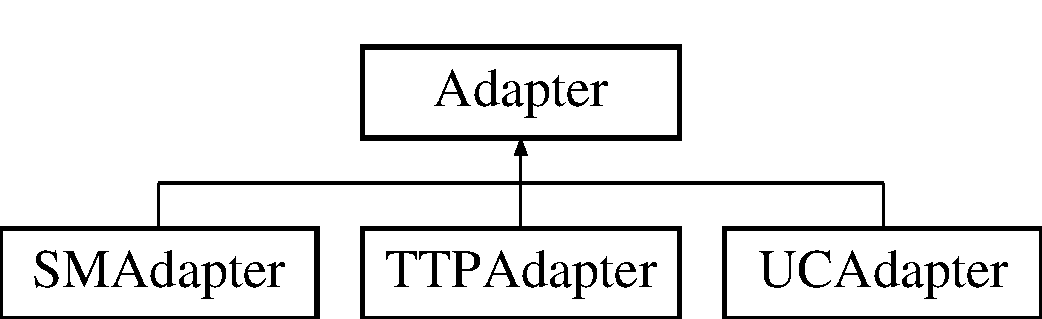
\includegraphics[height=2.000000cm]{classAdapter}
\end{center}
\end{figure}
\subsection*{Public Member Functions}
\begin{DoxyCompactItemize}
\item 
\hyperlink{classAdapter_a8c1799a1bd84d52fc7cbd8ebd07734eb}{Adapter} (\hyperlink{classsmart3p_1_1Unit}{smart3p\+::\+Unit} $\ast$o=N\+U\+LL)
\begin{DoxyCompactList}\small\item\em Constructor. \end{DoxyCompactList}\item 
virtual \hyperlink{classAdapter_a08a07acff57eb40aba27455de23ed13c}{$\sim$\+Adapter} ()
\begin{DoxyCompactList}\small\item\em Destructor. \end{DoxyCompactList}\item 
void \hyperlink{classAdapter_af928c4508bc6a76e8f9b918d38ffd221}{print} (char $\ast$)
\begin{DoxyCompactList}\small\item\em Simulation string output. \end{DoxyCompactList}\item 
void \hyperlink{classAdapter_a411c5677216438c68fc06f29909bf124}{print} (char $\ast$, Crypto\+P\+P\+::\+Integer $\ast$)
\begin{DoxyCompactList}\small\item\em Simulation Crypto\+P\+P\+::\+Integer output. \end{DoxyCompactList}\end{DoxyCompactItemize}
\subsection*{Static Public Member Functions}
\begin{DoxyCompactItemize}
\item 
static unsigned char $\ast$ \hyperlink{classAdapter_ae68c18841f3a26166d58e5771726a90e}{itob} (Crypto\+P\+P\+::\+Integer i)
\begin{DoxyCompactList}\small\item\em Utility function to convert from Crypto\+P\+P\+::\+Integer to unsigned char array. \end{DoxyCompactList}\item 
static const char $\ast$ \hyperlink{classAdapter_a670343c730c9d4b08cc98b5b58a65988}{itob\+Const} (Crypto\+P\+P\+::\+Integer i)
\begin{DoxyCompactList}\small\item\em Const variation of \hyperlink{classAdapter_ae68c18841f3a26166d58e5771726a90e}{itob(\+Crypto\+P\+P\+::\+Integer i)}. \end{DoxyCompactList}\item 
static Crypto\+P\+P\+::\+Integer \hyperlink{classAdapter_ac816b07d03c876f535286cd757a0995b}{btoi} (unsigned char $\ast$b, int length)
\begin{DoxyCompactList}\small\item\em Utility function to convert from unsigned character array to Crypto\+P\+P\+::\+Integer. \end{DoxyCompactList}\item 
static Crypto\+P\+P\+::\+Integer \hyperlink{classAdapter_aafe53d6cbf771b802c76236c05df1616}{btoi} (const char $\ast$b, int length)
\begin{DoxyCompactList}\small\item\em Const variation of \hyperlink{classAdapter_ac816b07d03c876f535286cd757a0995b}{btoi(unsigned char$\ast$ b, int length)}. \end{DoxyCompactList}\end{DoxyCompactItemize}
\subsection*{Protected Attributes}
\begin{DoxyCompactItemize}
\item 
bool \hyperlink{classAdapter_a49cad2fc1742424ec9f28caaa30f489f}{verbose}
\begin{DoxyCompactList}\small\item\em Verbose flag. \end{DoxyCompactList}\item 
\hyperlink{classsmart3p_1_1Unit}{smart3p\+::\+Unit} $\ast$ \hyperlink{classAdapter_abdeff6c9fdf71ac88a56318fa7aea4c4}{out}
\begin{DoxyCompactList}\small\item\em Simulation \hyperlink{classsmart3p_1_1Unit}{smart3p\+::\+Unit} Class. \end{DoxyCompactList}\end{DoxyCompactItemize}


\subsection{Detailed Description}
\hyperlink{classAdapter}{Adapter} Class. 

Abstract \hyperlink{classAdapter}{Adapter} class to convert between types used in the Protocol Implementation and the Simulation. Most of the protocol functionality shouldn\textquotesingle{}t occur here, as this is just a method to convert between types as well as pack/unpack packets and messages. This is designed to be extended and used by specific Adapters for each pair of classes to be \char`\"{}bridged\char`\"{}. \begin{DoxySeeAlso}{See also}
\hyperlink{classSMAdapter}{S\+M\+Adapter}, \hyperlink{classUCAdapter}{U\+C\+Adapter} and \hyperlink{classTTPAdapter}{T\+T\+P\+Adapter} 
\end{DoxySeeAlso}


Definition at line 30 of file Adapter.\+h.



\subsection{Constructor \& Destructor Documentation}
\mbox{\Hypertarget{classAdapter_a8c1799a1bd84d52fc7cbd8ebd07734eb}\label{classAdapter_a8c1799a1bd84d52fc7cbd8ebd07734eb}} 
\index{Adapter@{Adapter}!Adapter@{Adapter}}
\index{Adapter@{Adapter}!Adapter@{Adapter}}
\subsubsection{\texorpdfstring{Adapter()}{Adapter()}}
{\footnotesize\ttfamily Adapter\+::\+Adapter (\begin{DoxyParamCaption}\item[{\hyperlink{classsmart3p_1_1Unit}{smart3p\+::\+Unit} $\ast$}]{o = {\ttfamily NULL} }\end{DoxyParamCaption})}



Constructor. 

Constructor for the \hyperlink{classAdapter}{Adapter}. 
\begin{DoxyParams}{Parameters}
{\em o} & Sets the output \hyperlink{classsmart3p_1_1Unit}{smart3p\+::\+Unit} class. Sets the verbose flag to true if not N\+U\+LL. \\
\hline
\end{DoxyParams}


Definition at line 15 of file Adapter.\+cc.



References out, and verbose.

\mbox{\Hypertarget{classAdapter_a08a07acff57eb40aba27455de23ed13c}\label{classAdapter_a08a07acff57eb40aba27455de23ed13c}} 
\index{Adapter@{Adapter}!````~Adapter@{$\sim$\+Adapter}}
\index{````~Adapter@{$\sim$\+Adapter}!Adapter@{Adapter}}
\subsubsection{\texorpdfstring{$\sim$\+Adapter()}{~Adapter()}}
{\footnotesize\ttfamily Adapter\+::$\sim$\+Adapter (\begin{DoxyParamCaption}{ }\end{DoxyParamCaption})\hspace{0.3cm}{\ttfamily [virtual]}}



Destructor. 



Definition at line 21 of file Adapter.\+cc.



References out.



\subsection{Member Function Documentation}
\mbox{\Hypertarget{classAdapter_ac816b07d03c876f535286cd757a0995b}\label{classAdapter_ac816b07d03c876f535286cd757a0995b}} 
\index{Adapter@{Adapter}!btoi@{btoi}}
\index{btoi@{btoi}!Adapter@{Adapter}}
\subsubsection{\texorpdfstring{btoi()}{btoi()}\hspace{0.1cm}{\footnotesize\ttfamily [1/2]}}
{\footnotesize\ttfamily static Crypto\+P\+P\+::\+Integer Adapter\+::btoi (\begin{DoxyParamCaption}\item[{unsigned char $\ast$}]{b,  }\item[{int}]{length }\end{DoxyParamCaption})\hspace{0.3cm}{\ttfamily [inline]}, {\ttfamily [static]}}



Utility function to convert from unsigned character array to Crypto\+P\+P\+::\+Integer. 

Converts from unsigned character array to Crypto\+P\+P\+::\+Integer. 
\begin{DoxyParams}{Parameters}
{\em b} & unsigned char array. \\
\hline
{\em length} & Total length of the array. \\
\hline
\end{DoxyParams}
\begin{DoxyReturn}{Returns}
Returns new instance of Crypto\+P\+P\+::\+Integer. 
\end{DoxyReturn}
\begin{DoxySeeAlso}{See also}
\hyperlink{classAdapter_ae68c18841f3a26166d58e5771726a90e}{itob(\+Crypto\+P\+P\+::\+Integer i)} and \hyperlink{classAdapter_aafe53d6cbf771b802c76236c05df1616}{btoi(const char$\ast$ b, int length)} 
\end{DoxySeeAlso}


Definition at line 105 of file Adapter.\+h.

\mbox{\Hypertarget{classAdapter_aafe53d6cbf771b802c76236c05df1616}\label{classAdapter_aafe53d6cbf771b802c76236c05df1616}} 
\index{Adapter@{Adapter}!btoi@{btoi}}
\index{btoi@{btoi}!Adapter@{Adapter}}
\subsubsection{\texorpdfstring{btoi()}{btoi()}\hspace{0.1cm}{\footnotesize\ttfamily [2/2]}}
{\footnotesize\ttfamily static Crypto\+P\+P\+::\+Integer Adapter\+::btoi (\begin{DoxyParamCaption}\item[{const char $\ast$}]{b,  }\item[{int}]{length }\end{DoxyParamCaption})\hspace{0.3cm}{\ttfamily [inline]}, {\ttfamily [static]}}



Const variation of \hyperlink{classAdapter_ac816b07d03c876f535286cd757a0995b}{btoi(unsigned char$\ast$ b, int length)}. 



Definition at line 113 of file Adapter.\+h.

\mbox{\Hypertarget{classAdapter_ae68c18841f3a26166d58e5771726a90e}\label{classAdapter_ae68c18841f3a26166d58e5771726a90e}} 
\index{Adapter@{Adapter}!itob@{itob}}
\index{itob@{itob}!Adapter@{Adapter}}
\subsubsection{\texorpdfstring{itob()}{itob()}}
{\footnotesize\ttfamily static unsigned char$\ast$ Adapter\+::itob (\begin{DoxyParamCaption}\item[{Crypto\+P\+P\+::\+Integer}]{i }\end{DoxyParamCaption})\hspace{0.3cm}{\ttfamily [inline]}, {\ttfamily [static]}}



Utility function to convert from Crypto\+P\+P\+::\+Integer to unsigned char array. 

Converts Crypto\+P\+P\+::\+Integer to unsigned char array. Use Crypto\+P\+P\+::\+Integer.\+Byte\+Count() to get the size of the array. 
\begin{DoxyParams}{Parameters}
{\em i} & Crypto\+P\+P\+::\+Integer to convert. \\
\hline
\end{DoxyParams}
\begin{DoxyReturn}{Returns}
Returns unsigned char array. Use Crypto\+P\+P\+::\+Integer.\+Byte\+Count() to get the size of the array. 
\end{DoxyReturn}
\begin{DoxySeeAlso}{See also}
\hyperlink{classAdapter_ac816b07d03c876f535286cd757a0995b}{btoi(unsigned char$\ast$ b, int length)} and \hyperlink{classAdapter_a670343c730c9d4b08cc98b5b58a65988}{itob\+Const(\+Crypto\+P\+P\+::\+Integer i)} 
\end{DoxySeeAlso}


Definition at line 81 of file Adapter.\+h.

\mbox{\Hypertarget{classAdapter_a670343c730c9d4b08cc98b5b58a65988}\label{classAdapter_a670343c730c9d4b08cc98b5b58a65988}} 
\index{Adapter@{Adapter}!itob\+Const@{itob\+Const}}
\index{itob\+Const@{itob\+Const}!Adapter@{Adapter}}
\subsubsection{\texorpdfstring{itob\+Const()}{itobConst()}}
{\footnotesize\ttfamily static const char$\ast$ Adapter\+::itob\+Const (\begin{DoxyParamCaption}\item[{Crypto\+P\+P\+::\+Integer}]{i }\end{DoxyParamCaption})\hspace{0.3cm}{\ttfamily [inline]}, {\ttfamily [static]}}



Const variation of \hyperlink{classAdapter_ae68c18841f3a26166d58e5771726a90e}{itob(\+Crypto\+P\+P\+::\+Integer i)}. 



Definition at line 89 of file Adapter.\+h.

\mbox{\Hypertarget{classAdapter_af928c4508bc6a76e8f9b918d38ffd221}\label{classAdapter_af928c4508bc6a76e8f9b918d38ffd221}} 
\index{Adapter@{Adapter}!print@{print}}
\index{print@{print}!Adapter@{Adapter}}
\subsubsection{\texorpdfstring{print()}{print()}\hspace{0.1cm}{\footnotesize\ttfamily [1/2]}}
{\footnotesize\ttfamily void Adapter\+::print (\begin{DoxyParamCaption}\item[{char $\ast$}]{m }\end{DoxyParamCaption})}



Simulation string output. 

Prints the char string to the simulation output. Intended for debugging. \begin{DoxySeeAlso}{See also}
\hyperlink{classAdapter}{Adapter}(\hyperlink{classsmart3p_1_1Unit}{smart3p\+::\+Unit}$\ast$ o = N\+U\+LL), \hyperlink{classAdapter_af928c4508bc6a76e8f9b918d38ffd221}{print(char$\ast$)} and \hyperlink{classAdapter_a411c5677216438c68fc06f29909bf124}{print(char$\ast$, Crypto\+P\+P\+::\+Integer$\ast$)} 
\end{DoxySeeAlso}


Definition at line 26 of file Adapter.\+cc.



References D\+E\+B\+UG.

\mbox{\Hypertarget{classAdapter_a411c5677216438c68fc06f29909bf124}\label{classAdapter_a411c5677216438c68fc06f29909bf124}} 
\index{Adapter@{Adapter}!print@{print}}
\index{print@{print}!Adapter@{Adapter}}
\subsubsection{\texorpdfstring{print()}{print()}\hspace{0.1cm}{\footnotesize\ttfamily [2/2]}}
{\footnotesize\ttfamily void Adapter\+::print (\begin{DoxyParamCaption}\item[{char $\ast$}]{s,  }\item[{Crypto\+P\+P\+::\+Integer $\ast$}]{i }\end{DoxyParamCaption})}



Simulation Crypto\+P\+P\+::\+Integer output. 

Prints the provided Crypto\+P\+P\+::\+Integer to the simulation output as hex. Prepending the provided char string. Intended usage\+: print(\char`\"{}\+A large number\+: \char`\"{}, new Crypto\+P\+P\+::\+Integer(1234566789)); \begin{DoxySeeAlso}{See also}
\hyperlink{classAdapter}{Adapter}(\hyperlink{classsmart3p_1_1Unit}{smart3p\+::\+Unit}$\ast$ o = N\+U\+LL), \hyperlink{classAdapter_af928c4508bc6a76e8f9b918d38ffd221}{print(char$\ast$)} and \hyperlink{classAdapter_a411c5677216438c68fc06f29909bf124}{print(char$\ast$, Crypto\+P\+P\+::\+Integer$\ast$)} 
\end{DoxySeeAlso}


Definition at line 31 of file Adapter.\+cc.



References D\+E\+B\+UG.



\subsection{Field Documentation}
\mbox{\Hypertarget{classAdapter_abdeff6c9fdf71ac88a56318fa7aea4c4}\label{classAdapter_abdeff6c9fdf71ac88a56318fa7aea4c4}} 
\index{Adapter@{Adapter}!out@{out}}
\index{out@{out}!Adapter@{Adapter}}
\subsubsection{\texorpdfstring{out}{out}}
{\footnotesize\ttfamily \hyperlink{classsmart3p_1_1Unit}{smart3p\+::\+Unit}$\ast$ Adapter\+::out\hspace{0.3cm}{\ttfamily [protected]}}



Simulation \hyperlink{classsmart3p_1_1Unit}{smart3p\+::\+Unit} Class. 

This is a pointer to the Simulation-\/level abstract \hyperlink{classsmart3p_1_1Unit}{smart3p\+::\+Unit} class which provides debug output. Deprecated\+: Currently is also used as the output for emitting data thereby making its inclusion required. \begin{DoxySeeAlso}{See also}
\hyperlink{classAdapter}{Adapter}(\hyperlink{classsmart3p_1_1Unit}{smart3p\+::\+Unit}$\ast$ o = N\+U\+LL), \hyperlink{classAdapter_af928c4508bc6a76e8f9b918d38ffd221}{print(char$\ast$)} and \hyperlink{classAdapter_a411c5677216438c68fc06f29909bf124}{print(char$\ast$, Crypto\+P\+P\+::\+Integer$\ast$)} 
\end{DoxySeeAlso}


Definition at line 45 of file Adapter.\+h.

\mbox{\Hypertarget{classAdapter_a49cad2fc1742424ec9f28caaa30f489f}\label{classAdapter_a49cad2fc1742424ec9f28caaa30f489f}} 
\index{Adapter@{Adapter}!verbose@{verbose}}
\index{verbose@{verbose}!Adapter@{Adapter}}
\subsubsection{\texorpdfstring{verbose}{verbose}}
{\footnotesize\ttfamily bool Adapter\+::verbose\hspace{0.3cm}{\ttfamily [protected]}}



Verbose flag. 

A flag to offer some control over debug and other verbose output. 

Definition at line 37 of file Adapter.\+h.



The documentation for this class was generated from the following files\+:\begin{DoxyCompactItemize}
\item 
src/\hyperlink{Adapter_8h}{Adapter.\+h}\item 
src/\hyperlink{Adapter_8cc}{Adapter.\+cc}\end{DoxyCompactItemize}

\hypertarget{classcInteger}{}\section{c\+Integer Class Reference}
\label{classcInteger}\index{c\+Integer@{c\+Integer}}


A hybrid class between omnetpp\+::c\+Named\+Object and Crypto\+P\+P\+::\+Integer.  




{\ttfamily \#include $<$c\+Integer.\+h$>$}

Inheritance diagram for c\+Integer\+:\begin{figure}[H]
\begin{center}
\leavevmode
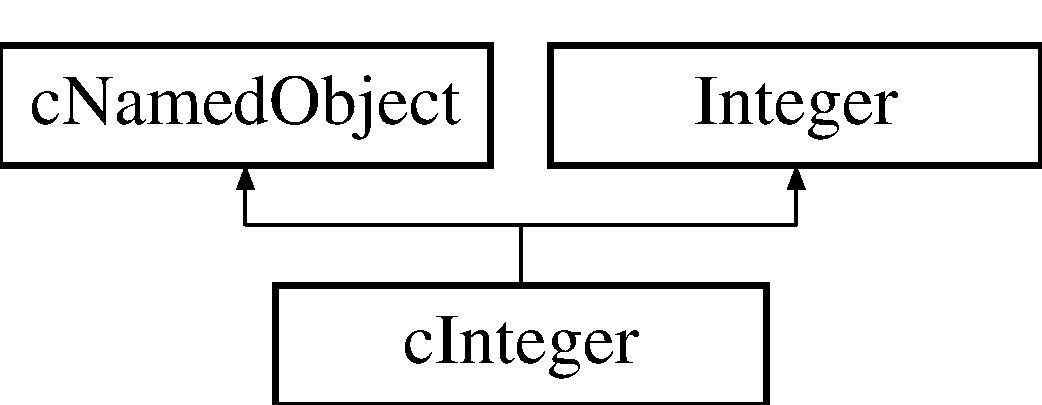
\includegraphics[height=2.000000cm]{classcInteger}
\end{center}
\end{figure}
\subsection*{Public Member Functions}
\begin{DoxyCompactItemize}
\item 
\hyperlink{classcInteger_afc876143cbe434def0b5851a98bc3ae8}{c\+Integer} (const char $\ast$n)
\begin{DoxyCompactList}\small\item\em Constructor. \end{DoxyCompactList}\item 
\hyperlink{classcInteger_a31669ca6b9b7f41f906320aaee8c8082}{c\+Integer} (const char $\ast$n, Crypto\+P\+P\+::\+Integer $\ast$i)
\begin{DoxyCompactList}\small\item\em Constructor. \end{DoxyCompactList}\item 
\hyperlink{classcInteger_aca26b0880fd20e8a87dbb435f29af348}{c\+Integer} (const char $\ast$n, int i)
\begin{DoxyCompactList}\small\item\em Constructor. \end{DoxyCompactList}\item 
\hyperlink{classcInteger_ad47b8fb0711aefe0d10fa8903d8ed6ca}{c\+Integer} (\hyperlink{classcInteger}{c\+Integer} $\ast$i)
\begin{DoxyCompactList}\small\item\em Constructor. \end{DoxyCompactList}\item 
virtual \hyperlink{classcInteger_a1e180c1db8ea39ad751a67e368a72465}{$\sim$c\+Integer} ()
\begin{DoxyCompactList}\small\item\em Destructor. \end{DoxyCompactList}\item 
const char $\ast$ \hyperlink{classcInteger_afd31eb924e2bfcc90f4a436acd4a827d}{get\+Class\+Name} () const
\item 
const char $\ast$ \hyperlink{classcInteger_ae6bb8246d4f19d41db22ffef801afd7c}{get\+Name} () const
\item 
void \hyperlink{classcInteger_aba2e5e7f13408b2dbbaf4a8460affc3c}{set\+Name} (const char $\ast$c)
\item 
\hyperlink{classcInteger}{c\+Integer} $\ast$ \hyperlink{classcInteger_a5fb5092056503a1241fbde5d80ef21ff}{dup} () const
\begin{DoxyCompactList}\small\item\em Duplicate. \end{DoxyCompactList}\item 
Crypto\+P\+P\+::\+Integer $\ast$ \hyperlink{classcInteger_a902f278d935322e8cce372ad4c465393}{to\+Integer} ()
\item 
void \hyperlink{classcInteger_a79060a0e5c29e71e7ba0b8b2d509109a}{parsim\+Pack} (omnetpp\+::c\+Comm\+Buffer $\ast$buffer) const
\item 
void \hyperlink{classcInteger_a0ae9eac774b0a394737209727486f93f}{parsim\+Unpack} (omnetpp\+::c\+Comm\+Buffer $\ast$buffer)
\end{DoxyCompactItemize}


\subsection{Detailed Description}
A hybrid class between omnetpp\+::c\+Named\+Object and Crypto\+P\+P\+::\+Integer. 

Designed to allow the passing of Crypo\+P\+P\+::\+Integer into messages and packets to make implementing adapters easier. 

Definition at line 11 of file c\+Integer.\+h.



\subsection{Constructor \& Destructor Documentation}
\mbox{\Hypertarget{classcInteger_afc876143cbe434def0b5851a98bc3ae8}\label{classcInteger_afc876143cbe434def0b5851a98bc3ae8}} 
\index{c\+Integer@{c\+Integer}!c\+Integer@{c\+Integer}}
\index{c\+Integer@{c\+Integer}!c\+Integer@{c\+Integer}}
\subsubsection{\texorpdfstring{c\+Integer()}{cInteger()}\hspace{0.1cm}{\footnotesize\ttfamily [1/4]}}
{\footnotesize\ttfamily c\+Integer\+::c\+Integer (\begin{DoxyParamCaption}\item[{const char $\ast$}]{n }\end{DoxyParamCaption})}



Constructor. 

Value is dependant upon the default behavour for Crypto\+P\+P\+::\+Integer when instantiated without a value. 
\begin{DoxyParams}{Parameters}
{\em n} & Instance name. \\
\hline
\end{DoxyParams}
\begin{DoxySeeAlso}{See also}
\hyperlink{classcInteger_ad47b8fb0711aefe0d10fa8903d8ed6ca}{c\+Integer(c\+Integer$\ast$)}, \hyperlink{classcInteger_a31669ca6b9b7f41f906320aaee8c8082}{c\+Integer(const char$\ast$, Crypto\+P\+P\+::\+Integer$\ast$)} and \hyperlink{classcInteger_aca26b0880fd20e8a87dbb435f29af348}{c\+Integer(const char$\ast$ n, int i)} 
\end{DoxySeeAlso}


Definition at line 3 of file c\+Integer.\+cc.

\mbox{\Hypertarget{classcInteger_a31669ca6b9b7f41f906320aaee8c8082}\label{classcInteger_a31669ca6b9b7f41f906320aaee8c8082}} 
\index{c\+Integer@{c\+Integer}!c\+Integer@{c\+Integer}}
\index{c\+Integer@{c\+Integer}!c\+Integer@{c\+Integer}}
\subsubsection{\texorpdfstring{c\+Integer()}{cInteger()}\hspace{0.1cm}{\footnotesize\ttfamily [2/4]}}
{\footnotesize\ttfamily c\+Integer\+::c\+Integer (\begin{DoxyParamCaption}\item[{const char $\ast$}]{n,  }\item[{Crypto\+P\+P\+::\+Integer $\ast$}]{i }\end{DoxyParamCaption})}



Constructor. 


\begin{DoxyParams}{Parameters}
{\em n} & Instance name. \\
\hline
{\em i} & copies provided Crypto\+P\+P\+::\+Integer. \\
\hline
\end{DoxyParams}
\begin{DoxySeeAlso}{See also}
\hyperlink{classcInteger_afc876143cbe434def0b5851a98bc3ae8}{c\+Integer(const char$\ast$ n)}, \hyperlink{classcInteger_ad47b8fb0711aefe0d10fa8903d8ed6ca}{c\+Integer(c\+Integer$\ast$)}, and \hyperlink{classcInteger_aca26b0880fd20e8a87dbb435f29af348}{c\+Integer(const char$\ast$ n, int i)} 
\end{DoxySeeAlso}


Definition at line 8 of file c\+Integer.\+cc.

\mbox{\Hypertarget{classcInteger_aca26b0880fd20e8a87dbb435f29af348}\label{classcInteger_aca26b0880fd20e8a87dbb435f29af348}} 
\index{c\+Integer@{c\+Integer}!c\+Integer@{c\+Integer}}
\index{c\+Integer@{c\+Integer}!c\+Integer@{c\+Integer}}
\subsubsection{\texorpdfstring{c\+Integer()}{cInteger()}\hspace{0.1cm}{\footnotesize\ttfamily [3/4]}}
{\footnotesize\ttfamily c\+Integer\+::c\+Integer (\begin{DoxyParamCaption}\item[{const char $\ast$}]{n,  }\item[{int}]{i }\end{DoxyParamCaption})}



Constructor. 


\begin{DoxyParams}{Parameters}
{\em n} & Instance name. \\
\hline
{\em i} & Value \\
\hline
\end{DoxyParams}
\begin{DoxySeeAlso}{See also}
\hyperlink{classcInteger_afc876143cbe434def0b5851a98bc3ae8}{c\+Integer(const char$\ast$ n)}, \hyperlink{classcInteger_ad47b8fb0711aefe0d10fa8903d8ed6ca}{c\+Integer(c\+Integer$\ast$)}, and \hyperlink{classcInteger_a31669ca6b9b7f41f906320aaee8c8082}{c\+Integer(const char$\ast$, Crypto\+P\+P\+::\+Integer$\ast$)} 
\end{DoxySeeAlso}


Definition at line 13 of file c\+Integer.\+cc.

\mbox{\Hypertarget{classcInteger_ad47b8fb0711aefe0d10fa8903d8ed6ca}\label{classcInteger_ad47b8fb0711aefe0d10fa8903d8ed6ca}} 
\index{c\+Integer@{c\+Integer}!c\+Integer@{c\+Integer}}
\index{c\+Integer@{c\+Integer}!c\+Integer@{c\+Integer}}
\subsubsection{\texorpdfstring{c\+Integer()}{cInteger()}\hspace{0.1cm}{\footnotesize\ttfamily [4/4]}}
{\footnotesize\ttfamily c\+Integer\+::c\+Integer (\begin{DoxyParamCaption}\item[{\hyperlink{classcInteger}{c\+Integer} $\ast$}]{i }\end{DoxyParamCaption})}



Constructor. 

Copy constructor. \begin{DoxySeeAlso}{See also}
\hyperlink{classcInteger_afc876143cbe434def0b5851a98bc3ae8}{c\+Integer(const char$\ast$ n)}, \hyperlink{classcInteger_a31669ca6b9b7f41f906320aaee8c8082}{c\+Integer(const char$\ast$, Crypto\+P\+P\+::\+Integer$\ast$)} and \hyperlink{classcInteger_aca26b0880fd20e8a87dbb435f29af348}{c\+Integer(const char$\ast$ n, int i)} 
\end{DoxySeeAlso}


Definition at line 18 of file c\+Integer.\+cc.



References get\+Name().

\mbox{\Hypertarget{classcInteger_a1e180c1db8ea39ad751a67e368a72465}\label{classcInteger_a1e180c1db8ea39ad751a67e368a72465}} 
\index{c\+Integer@{c\+Integer}!````~c\+Integer@{$\sim$c\+Integer}}
\index{````~c\+Integer@{$\sim$c\+Integer}!c\+Integer@{c\+Integer}}
\subsubsection{\texorpdfstring{$\sim$c\+Integer()}{~cInteger()}}
{\footnotesize\ttfamily c\+Integer\+::$\sim$c\+Integer (\begin{DoxyParamCaption}{ }\end{DoxyParamCaption})\hspace{0.3cm}{\ttfamily [virtual]}}



Destructor. 



Definition at line 24 of file c\+Integer.\+cc.



\subsection{Member Function Documentation}
\mbox{\Hypertarget{classcInteger_a5fb5092056503a1241fbde5d80ef21ff}\label{classcInteger_a5fb5092056503a1241fbde5d80ef21ff}} 
\index{c\+Integer@{c\+Integer}!dup@{dup}}
\index{dup@{dup}!c\+Integer@{c\+Integer}}
\subsubsection{\texorpdfstring{dup()}{dup()}}
{\footnotesize\ttfamily \hyperlink{classcInteger}{c\+Integer} $\ast$ c\+Integer\+::dup (\begin{DoxyParamCaption}{ }\end{DoxyParamCaption}) const}



Duplicate. 

Provides a duplication of the class (via the copy constructor). \begin{DoxyReturn}{Returns}
A new copy of this instance. 
\end{DoxyReturn}


Definition at line 42 of file c\+Integer.\+cc.



References c\+Integer().

\mbox{\Hypertarget{classcInteger_afd31eb924e2bfcc90f4a436acd4a827d}\label{classcInteger_afd31eb924e2bfcc90f4a436acd4a827d}} 
\index{c\+Integer@{c\+Integer}!get\+Class\+Name@{get\+Class\+Name}}
\index{get\+Class\+Name@{get\+Class\+Name}!c\+Integer@{c\+Integer}}
\subsubsection{\texorpdfstring{get\+Class\+Name()}{getClassName()}}
{\footnotesize\ttfamily const char $\ast$ c\+Integer\+::get\+Class\+Name (\begin{DoxyParamCaption}{ }\end{DoxyParamCaption}) const}

\begin{DoxyReturn}{Returns}
Returns class\+Name. 
\end{DoxyReturn}
\begin{DoxySeeAlso}{See also}
class\+Name 
\end{DoxySeeAlso}


Definition at line 28 of file c\+Integer.\+cc.

\mbox{\Hypertarget{classcInteger_ae6bb8246d4f19d41db22ffef801afd7c}\label{classcInteger_ae6bb8246d4f19d41db22ffef801afd7c}} 
\index{c\+Integer@{c\+Integer}!get\+Name@{get\+Name}}
\index{get\+Name@{get\+Name}!c\+Integer@{c\+Integer}}
\subsubsection{\texorpdfstring{get\+Name()}{getName()}}
{\footnotesize\ttfamily const char $\ast$ c\+Integer\+::get\+Name (\begin{DoxyParamCaption}{ }\end{DoxyParamCaption}) const}

\begin{DoxyReturn}{Returns}
Returns instance name. 
\end{DoxyReturn}
\begin{DoxySeeAlso}{See also}
\hyperlink{classcInteger_aba2e5e7f13408b2dbbaf4a8460affc3c}{set\+Name(const char$\ast$)}. 
\end{DoxySeeAlso}


Definition at line 32 of file c\+Integer.\+cc.

\mbox{\Hypertarget{classcInteger_a79060a0e5c29e71e7ba0b8b2d509109a}\label{classcInteger_a79060a0e5c29e71e7ba0b8b2d509109a}} 
\index{c\+Integer@{c\+Integer}!parsim\+Pack@{parsim\+Pack}}
\index{parsim\+Pack@{parsim\+Pack}!c\+Integer@{c\+Integer}}
\subsubsection{\texorpdfstring{parsim\+Pack()}{parsimPack()}}
{\footnotesize\ttfamily void c\+Integer\+::parsim\+Pack (\begin{DoxyParamCaption}\item[{omnetpp\+::c\+Comm\+Buffer $\ast$}]{buffer }\end{DoxyParamCaption}) const}

Packs the class into an omnetpp\+::c\+Comm\+Buffer allowing for parallelization. 
\begin{DoxyParams}{Parameters}
{\em buffer} & The buffer to pack into. \\
\hline
\end{DoxyParams}


Definition at line 52 of file c\+Integer.\+cc.

\mbox{\Hypertarget{classcInteger_a0ae9eac774b0a394737209727486f93f}\label{classcInteger_a0ae9eac774b0a394737209727486f93f}} 
\index{c\+Integer@{c\+Integer}!parsim\+Unpack@{parsim\+Unpack}}
\index{parsim\+Unpack@{parsim\+Unpack}!c\+Integer@{c\+Integer}}
\subsubsection{\texorpdfstring{parsim\+Unpack()}{parsimUnpack()}}
{\footnotesize\ttfamily void c\+Integer\+::parsim\+Unpack (\begin{DoxyParamCaption}\item[{omnetpp\+::c\+Comm\+Buffer $\ast$}]{buffer }\end{DoxyParamCaption})}

Unpacks the class from an omnetpp\+::c\+Comm\+Buffer allowing for parallelization. 
\begin{DoxyParams}{Parameters}
{\em buffer} & The buffer to pack from. \\
\hline
\end{DoxyParams}


Definition at line 64 of file c\+Integer.\+cc.

\mbox{\Hypertarget{classcInteger_aba2e5e7f13408b2dbbaf4a8460affc3c}\label{classcInteger_aba2e5e7f13408b2dbbaf4a8460affc3c}} 
\index{c\+Integer@{c\+Integer}!set\+Name@{set\+Name}}
\index{set\+Name@{set\+Name}!c\+Integer@{c\+Integer}}
\subsubsection{\texorpdfstring{set\+Name()}{setName()}}
{\footnotesize\ttfamily void c\+Integer\+::set\+Name (\begin{DoxyParamCaption}\item[{const char $\ast$}]{c }\end{DoxyParamCaption})}

Sets the name of the instance. 
\begin{DoxyParams}{Parameters}
{\em c} & const char string to change the name to. \\
\hline
\end{DoxyParams}
\begin{DoxySeeAlso}{See also}
\hyperlink{classcInteger_ae6bb8246d4f19d41db22ffef801afd7c}{get\+Name()} 
\end{DoxySeeAlso}


Definition at line 37 of file c\+Integer.\+cc.

\mbox{\Hypertarget{classcInteger_a902f278d935322e8cce372ad4c465393}\label{classcInteger_a902f278d935322e8cce372ad4c465393}} 
\index{c\+Integer@{c\+Integer}!to\+Integer@{to\+Integer}}
\index{to\+Integer@{to\+Integer}!c\+Integer@{c\+Integer}}
\subsubsection{\texorpdfstring{to\+Integer()}{toInteger()}}
{\footnotesize\ttfamily Crypto\+P\+P\+::\+Integer $\ast$ c\+Integer\+::to\+Integer (\begin{DoxyParamCaption}{ }\end{DoxyParamCaption})}

dynamic casts to a Crypto\+P\+P\+::\+Integer 

Definition at line 47 of file c\+Integer.\+cc.



The documentation for this class was generated from the following files\+:\begin{DoxyCompactItemize}
\item 
src/\hyperlink{cInteger_8h}{c\+Integer.\+h}\item 
src/\hyperlink{cInteger_8cc}{c\+Integer.\+cc}\end{DoxyCompactItemize}

\hypertarget{classsmart3p_1_1Collector}{}\section{smart3p\+:\+:Collector Class Reference}
\label{classsmart3p_1_1Collector}\index{smart3p\+::\+Collector@{smart3p\+::\+Collector}}


\hyperlink{classsmart3p_1_1Collector}{Collector} for \hyperlink{classsmart3p_1_1SmartMeter}{smart3p\+::\+Smart\+Meter}.  




{\ttfamily \#include $<$Collector.\+h$>$}

Inheritance diagram for smart3p\+:\+:Collector\+:\begin{figure}[H]
\begin{center}
\leavevmode
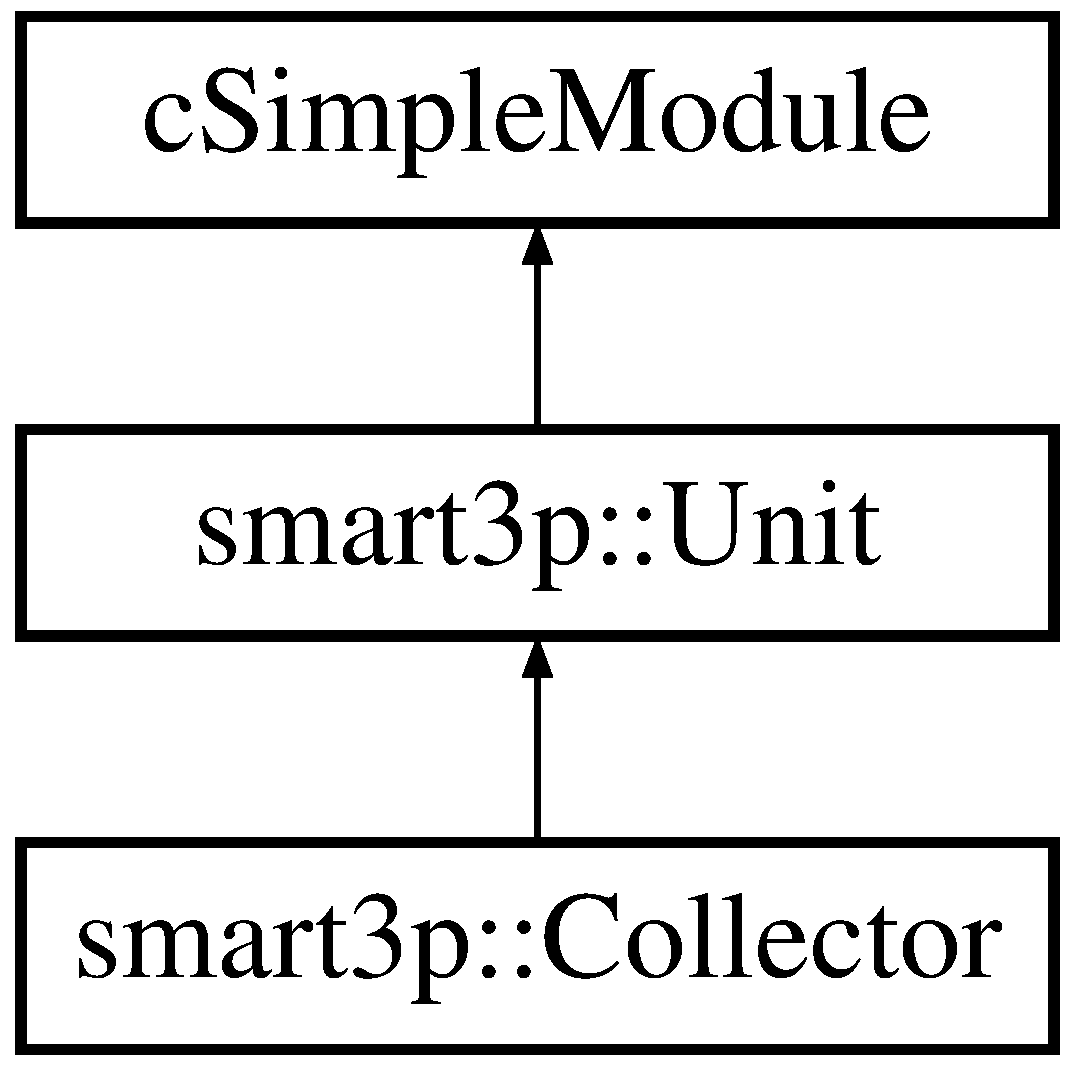
\includegraphics[height=3.000000cm]{classsmart3p_1_1Collector}
\end{center}
\end{figure}
\subsection*{Public Member Functions}
\begin{DoxyCompactItemize}
\item 
\hyperlink{classsmart3p_1_1Collector_afb4275cafc381a2650b7a6dd9465662e}{Collector} ()
\item 
virtual \hyperlink{classsmart3p_1_1Collector_a650466fb964d056afb0f35b1d6966e7c}{$\sim$\+Collector} ()
\end{DoxyCompactItemize}
\subsection*{Protected Member Functions}
\begin{DoxyCompactItemize}
\item 
virtual void \hyperlink{classsmart3p_1_1Collector_acc6c1b2f235b3c4acb7ca84f7c356e80}{initialize} ()
\item 
virtual void \hyperlink{classsmart3p_1_1Collector_a1b82f1a10a2579c3ed25bc899220b906}{timed\+Handle\+Message} (c\+Message $\ast$msg)
\end{DoxyCompactItemize}
\subsection*{Additional Inherited Members}


\subsection{Detailed Description}
\hyperlink{classsmart3p_1_1Collector}{Collector} for \hyperlink{classsmart3p_1_1SmartMeter}{smart3p\+::\+Smart\+Meter}. 

Collects messages \hyperlink{classsmart3p_1_1SmartMeter}{smart3p\+::\+Smart\+Meter} and forwards them to the \hyperlink{classsmart3p_1_1UtilityCompany}{smart3p\+::\+Utility\+Company}. 

Definition at line 16 of file Collector.\+h.



\subsection{Constructor \& Destructor Documentation}
\mbox{\Hypertarget{classsmart3p_1_1Collector_afb4275cafc381a2650b7a6dd9465662e}\label{classsmart3p_1_1Collector_afb4275cafc381a2650b7a6dd9465662e}} 
\index{smart3p\+::\+Collector@{smart3p\+::\+Collector}!Collector@{Collector}}
\index{Collector@{Collector}!smart3p\+::\+Collector@{smart3p\+::\+Collector}}
\subsubsection{\texorpdfstring{Collector()}{Collector()}}
{\footnotesize\ttfamily smart3p\+::\+Collector\+::\+Collector (\begin{DoxyParamCaption}{ }\end{DoxyParamCaption})}



Definition at line 11 of file Collector.\+cc.

\mbox{\Hypertarget{classsmart3p_1_1Collector_a650466fb964d056afb0f35b1d6966e7c}\label{classsmart3p_1_1Collector_a650466fb964d056afb0f35b1d6966e7c}} 
\index{smart3p\+::\+Collector@{smart3p\+::\+Collector}!````~Collector@{$\sim$\+Collector}}
\index{````~Collector@{$\sim$\+Collector}!smart3p\+::\+Collector@{smart3p\+::\+Collector}}
\subsubsection{\texorpdfstring{$\sim$\+Collector()}{~Collector()}}
{\footnotesize\ttfamily smart3p\+::\+Collector\+::$\sim$\+Collector (\begin{DoxyParamCaption}{ }\end{DoxyParamCaption})\hspace{0.3cm}{\ttfamily [virtual]}}



Definition at line 16 of file Collector.\+cc.



\subsection{Member Function Documentation}
\mbox{\Hypertarget{classsmart3p_1_1Collector_acc6c1b2f235b3c4acb7ca84f7c356e80}\label{classsmart3p_1_1Collector_acc6c1b2f235b3c4acb7ca84f7c356e80}} 
\index{smart3p\+::\+Collector@{smart3p\+::\+Collector}!initialize@{initialize}}
\index{initialize@{initialize}!smart3p\+::\+Collector@{smart3p\+::\+Collector}}
\subsubsection{\texorpdfstring{initialize()}{initialize()}}
{\footnotesize\ttfamily void smart3p\+::\+Collector\+::initialize (\begin{DoxyParamCaption}{ }\end{DoxyParamCaption})\hspace{0.3cm}{\ttfamily [protected]}, {\ttfamily [virtual]}}



Definition at line 21 of file Collector.\+cc.

\mbox{\Hypertarget{classsmart3p_1_1Collector_a1b82f1a10a2579c3ed25bc899220b906}\label{classsmart3p_1_1Collector_a1b82f1a10a2579c3ed25bc899220b906}} 
\index{smart3p\+::\+Collector@{smart3p\+::\+Collector}!timed\+Handle\+Message@{timed\+Handle\+Message}}
\index{timed\+Handle\+Message@{timed\+Handle\+Message}!smart3p\+::\+Collector@{smart3p\+::\+Collector}}
\subsubsection{\texorpdfstring{timed\+Handle\+Message()}{timedHandleMessage()}}
{\footnotesize\ttfamily void smart3p\+::\+Collector\+::timed\+Handle\+Message (\begin{DoxyParamCaption}\item[{c\+Message $\ast$}]{msg }\end{DoxyParamCaption})\hspace{0.3cm}{\ttfamily [protected]}, {\ttfamily [virtual]}}

Unused, simply prints te message name. 
\begin{DoxyParams}{Parameters}
{\em msg} & Input message to be handled. \\
\hline
\end{DoxyParams}


Reimplemented from \hyperlink{classsmart3p_1_1Unit_a93f16f43dec69d23d8588f3b60c96d69}{smart3p\+::\+Unit}.



Definition at line 26 of file Collector.\+cc.



References smart3p\+::\+S\+M\+Packet\+::get\+Sm\+Gate\+I\+D(), and smart3p\+::\+S\+M\+Packet\+::set\+Sm\+Gate\+I\+D().



The documentation for this class was generated from the following files\+:\begin{DoxyCompactItemize}
\item 
src/\hyperlink{Collector_8h}{Collector.\+h}\item 
src/\hyperlink{Collector_8cc}{Collector.\+cc}\end{DoxyCompactItemize}

\hypertarget{classsmart3p_1_1DataGenerator}{}\section{smart3p\+:\+:Data\+Generator Class Reference}
\label{classsmart3p_1_1DataGenerator}\index{smart3p\+::\+Data\+Generator@{smart3p\+::\+Data\+Generator}}


Generates data for \hyperlink{classsmart3p_1_1SmartMeter}{smart3p\+::\+Smart\+Meter}.  




{\ttfamily \#include $<$Data\+Generator.\+h$>$}

Inheritance diagram for smart3p\+:\+:Data\+Generator\+:\begin{figure}[H]
\begin{center}
\leavevmode
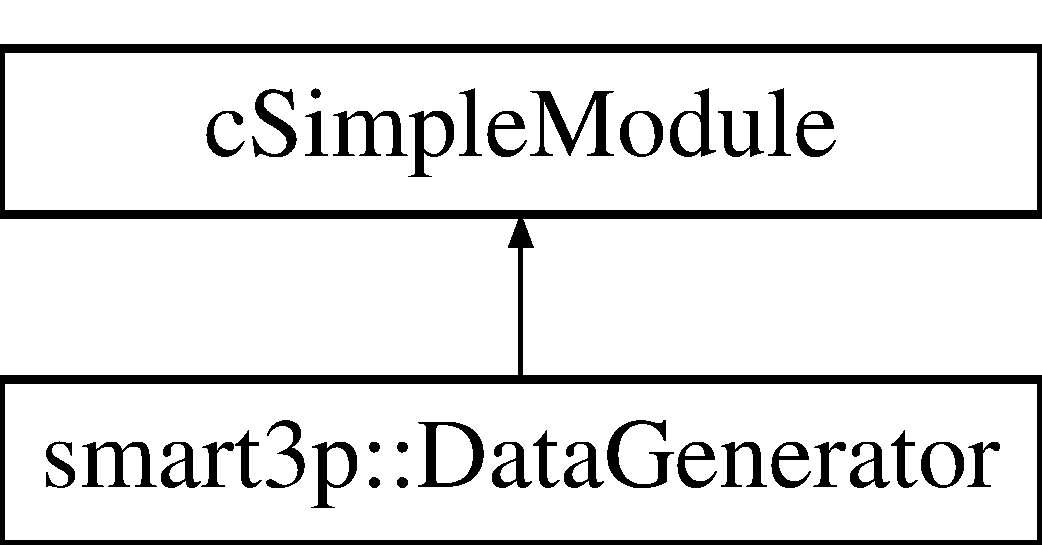
\includegraphics[height=2.000000cm]{classsmart3p_1_1DataGenerator}
\end{center}
\end{figure}
\subsection*{Protected Member Functions}
\begin{DoxyCompactItemize}
\item 
virtual void \hyperlink{classsmart3p_1_1DataGenerator_a0a4e7108a50c24c2485645d314892581}{initialize} ()
\begin{DoxyCompactList}\small\item\em Class initilization. \end{DoxyCompactList}\item 
virtual void \hyperlink{classsmart3p_1_1DataGenerator_a5a26a1e77fc192ce9024e9fad5b16a38}{handle\+Message} (c\+Message $\ast$msg)
\begin{DoxyCompactList}\small\item\em Main message handler. \end{DoxyCompactList}\item 
virtual void \hyperlink{classsmart3p_1_1DataGenerator_a30cad918b7a471eeec37508e7d4a9c07}{finish} ()
\begin{DoxyCompactList}\small\item\em Called when simulation is shut down. \end{DoxyCompactList}\end{DoxyCompactItemize}


\subsection{Detailed Description}
Generates data for \hyperlink{classsmart3p_1_1SmartMeter}{smart3p\+::\+Smart\+Meter}. 

Definition at line 14 of file Data\+Generator.\+h.



\subsection{Member Function Documentation}
\mbox{\Hypertarget{classsmart3p_1_1DataGenerator_a30cad918b7a471eeec37508e7d4a9c07}\label{classsmart3p_1_1DataGenerator_a30cad918b7a471eeec37508e7d4a9c07}} 
\index{smart3p\+::\+Data\+Generator@{smart3p\+::\+Data\+Generator}!finish@{finish}}
\index{finish@{finish}!smart3p\+::\+Data\+Generator@{smart3p\+::\+Data\+Generator}}
\subsubsection{\texorpdfstring{finish()}{finish()}}
{\footnotesize\ttfamily void smart3p\+::\+Data\+Generator\+::finish (\begin{DoxyParamCaption}{ }\end{DoxyParamCaption})\hspace{0.3cm}{\ttfamily [protected]}, {\ttfamily [virtual]}}



Called when simulation is shut down. 



Definition at line 214 of file Data\+Generator.\+cc.

\mbox{\Hypertarget{classsmart3p_1_1DataGenerator_a5a26a1e77fc192ce9024e9fad5b16a38}\label{classsmart3p_1_1DataGenerator_a5a26a1e77fc192ce9024e9fad5b16a38}} 
\index{smart3p\+::\+Data\+Generator@{smart3p\+::\+Data\+Generator}!handle\+Message@{handle\+Message}}
\index{handle\+Message@{handle\+Message}!smart3p\+::\+Data\+Generator@{smart3p\+::\+Data\+Generator}}
\subsubsection{\texorpdfstring{handle\+Message()}{handleMessage()}}
{\footnotesize\ttfamily void smart3p\+::\+Data\+Generator\+::handle\+Message (\begin{DoxyParamCaption}\item[{c\+Message $\ast$}]{msg }\end{DoxyParamCaption})\hspace{0.3cm}{\ttfamily [protected]}, {\ttfamily [virtual]}}



Main message handler. 



Definition at line 151 of file Data\+Generator.\+cc.



References smart3p\+::\+S\+M\+Packet\+::get\+Id(), and smart3p\+::\+S\+M\+Packet\+::set\+Id().

\mbox{\Hypertarget{classsmart3p_1_1DataGenerator_a0a4e7108a50c24c2485645d314892581}\label{classsmart3p_1_1DataGenerator_a0a4e7108a50c24c2485645d314892581}} 
\index{smart3p\+::\+Data\+Generator@{smart3p\+::\+Data\+Generator}!initialize@{initialize}}
\index{initialize@{initialize}!smart3p\+::\+Data\+Generator@{smart3p\+::\+Data\+Generator}}
\subsubsection{\texorpdfstring{initialize()}{initialize()}}
{\footnotesize\ttfamily void smart3p\+::\+Data\+Generator\+::initialize (\begin{DoxyParamCaption}{ }\end{DoxyParamCaption})\hspace{0.3cm}{\ttfamily [protected]}, {\ttfamily [virtual]}}



Class initilization. 



Definition at line 15 of file Data\+Generator.\+cc.



References smart3p\+::\+S\+M\+Packet\+::set\+Value().



The documentation for this class was generated from the following files\+:\begin{DoxyCompactItemize}
\item 
src/\hyperlink{DataGenerator_8h}{Data\+Generator.\+h}\item 
src/\hyperlink{DataGenerator_8cc}{Data\+Generator.\+cc}\end{DoxyCompactItemize}

\hypertarget{structSMImp_1_1HMACPayload}{}\section{S\+M\+Imp\+:\+:H\+M\+A\+C\+Payload Struct Reference}
\label{structSMImp_1_1HMACPayload}\index{S\+M\+Imp\+::\+H\+M\+A\+C\+Payload@{S\+M\+Imp\+::\+H\+M\+A\+C\+Payload}}


H\+M\+AC signed payload with encrypted elements.  




{\ttfamily \#include $<$examples.\+h$>$}

\subsection*{Data Fields}
\begin{DoxyCompactItemize}
\item 
Integer \hyperlink{structSMImp_1_1HMACPayload_a43ba32c0eb4fd4bd21de24aed393a0ae}{message\+Length}
\begin{DoxyCompactList}\small\item\em Total length of the message. \end{DoxyCompactList}\item 
Integer \hyperlink{structSMImp_1_1HMACPayload_a9c5590cfd65a39f500552ea95b583241}{hmac}
\begin{DoxyCompactList}\small\item\em Generated H\+M\+AC for verification. \end{DoxyCompactList}\item 
Integer \hyperlink{structSMImp_1_1HMACPayload_aa28e06eeacc346a1add298357a8b7fb9}{c1}
\begin{DoxyCompactList}\small\item\em Part 1 of the encrypted message. \end{DoxyCompactList}\item 
Integer \hyperlink{structSMImp_1_1HMACPayload_aeb2e7ef7dfeda975882a42aab9c0652f}{c2}
\begin{DoxyCompactList}\small\item\em Part 2 of the encrypted message. \end{DoxyCompactList}\item 
Integer \hyperlink{structSMImp_1_1HMACPayload_ab79ad3d823f9477a652bfd9b92f3c15b}{id}
\begin{DoxyCompactList}\small\item\em ID of the originating \hyperlink{classSMImp_1_1Requester}{Requester}. \end{DoxyCompactList}\item 
Integer \hyperlink{structSMImp_1_1HMACPayload_abf2b3077546fcf168ee7e0fe80a08b40}{time\+Stamp}
\begin{DoxyCompactList}\small\item\em Timestamp. \end{DoxyCompactList}\item 
Integer \hyperlink{structSMImp_1_1HMACPayload_a6829ee16dbd13177fdbca12b6e52a75b}{r}
\begin{DoxyCompactList}\small\item\em Shared secret, often unused. \end{DoxyCompactList}\end{DoxyCompactItemize}


\subsection{Detailed Description}
H\+M\+AC signed payload with encrypted elements. 

Definition at line 81 of file examples.\+h.



\subsection{Field Documentation}
\mbox{\Hypertarget{structSMImp_1_1HMACPayload_aa28e06eeacc346a1add298357a8b7fb9}\label{structSMImp_1_1HMACPayload_aa28e06eeacc346a1add298357a8b7fb9}} 
\index{S\+M\+Imp\+::\+H\+M\+A\+C\+Payload@{S\+M\+Imp\+::\+H\+M\+A\+C\+Payload}!c1@{c1}}
\index{c1@{c1}!S\+M\+Imp\+::\+H\+M\+A\+C\+Payload@{S\+M\+Imp\+::\+H\+M\+A\+C\+Payload}}
\subsubsection{\texorpdfstring{c1}{c1}}
{\footnotesize\ttfamily Integer S\+M\+Imp\+::\+H\+M\+A\+C\+Payload\+::c1}



Part 1 of the encrypted message. 



Definition at line 91 of file examples.\+h.

\mbox{\Hypertarget{structSMImp_1_1HMACPayload_aeb2e7ef7dfeda975882a42aab9c0652f}\label{structSMImp_1_1HMACPayload_aeb2e7ef7dfeda975882a42aab9c0652f}} 
\index{S\+M\+Imp\+::\+H\+M\+A\+C\+Payload@{S\+M\+Imp\+::\+H\+M\+A\+C\+Payload}!c2@{c2}}
\index{c2@{c2}!S\+M\+Imp\+::\+H\+M\+A\+C\+Payload@{S\+M\+Imp\+::\+H\+M\+A\+C\+Payload}}
\subsubsection{\texorpdfstring{c2}{c2}}
{\footnotesize\ttfamily Integer S\+M\+Imp\+::\+H\+M\+A\+C\+Payload\+::c2}



Part 2 of the encrypted message. 



Definition at line 93 of file examples.\+h.

\mbox{\Hypertarget{structSMImp_1_1HMACPayload_a9c5590cfd65a39f500552ea95b583241}\label{structSMImp_1_1HMACPayload_a9c5590cfd65a39f500552ea95b583241}} 
\index{S\+M\+Imp\+::\+H\+M\+A\+C\+Payload@{S\+M\+Imp\+::\+H\+M\+A\+C\+Payload}!hmac@{hmac}}
\index{hmac@{hmac}!S\+M\+Imp\+::\+H\+M\+A\+C\+Payload@{S\+M\+Imp\+::\+H\+M\+A\+C\+Payload}}
\subsubsection{\texorpdfstring{hmac}{hmac}}
{\footnotesize\ttfamily Integer S\+M\+Imp\+::\+H\+M\+A\+C\+Payload\+::hmac}



Generated H\+M\+AC for verification. 



Definition at line 89 of file examples.\+h.

\mbox{\Hypertarget{structSMImp_1_1HMACPayload_ab79ad3d823f9477a652bfd9b92f3c15b}\label{structSMImp_1_1HMACPayload_ab79ad3d823f9477a652bfd9b92f3c15b}} 
\index{S\+M\+Imp\+::\+H\+M\+A\+C\+Payload@{S\+M\+Imp\+::\+H\+M\+A\+C\+Payload}!id@{id}}
\index{id@{id}!S\+M\+Imp\+::\+H\+M\+A\+C\+Payload@{S\+M\+Imp\+::\+H\+M\+A\+C\+Payload}}
\subsubsection{\texorpdfstring{id}{id}}
{\footnotesize\ttfamily Integer S\+M\+Imp\+::\+H\+M\+A\+C\+Payload\+::id}



ID of the originating \hyperlink{classSMImp_1_1Requester}{Requester}. 



Definition at line 95 of file examples.\+h.

\mbox{\Hypertarget{structSMImp_1_1HMACPayload_a43ba32c0eb4fd4bd21de24aed393a0ae}\label{structSMImp_1_1HMACPayload_a43ba32c0eb4fd4bd21de24aed393a0ae}} 
\index{S\+M\+Imp\+::\+H\+M\+A\+C\+Payload@{S\+M\+Imp\+::\+H\+M\+A\+C\+Payload}!message\+Length@{message\+Length}}
\index{message\+Length@{message\+Length}!S\+M\+Imp\+::\+H\+M\+A\+C\+Payload@{S\+M\+Imp\+::\+H\+M\+A\+C\+Payload}}
\subsubsection{\texorpdfstring{message\+Length}{messageLength}}
{\footnotesize\ttfamily Integer S\+M\+Imp\+::\+H\+M\+A\+C\+Payload\+::message\+Length}



Total length of the message. 

Since fragmentation is possible, it\textquotesingle{}s important to know the totaly length of the overall message being sent. 

Definition at line 87 of file examples.\+h.

\mbox{\Hypertarget{structSMImp_1_1HMACPayload_a6829ee16dbd13177fdbca12b6e52a75b}\label{structSMImp_1_1HMACPayload_a6829ee16dbd13177fdbca12b6e52a75b}} 
\index{S\+M\+Imp\+::\+H\+M\+A\+C\+Payload@{S\+M\+Imp\+::\+H\+M\+A\+C\+Payload}!r@{r}}
\index{r@{r}!S\+M\+Imp\+::\+H\+M\+A\+C\+Payload@{S\+M\+Imp\+::\+H\+M\+A\+C\+Payload}}
\subsubsection{\texorpdfstring{r}{r}}
{\footnotesize\ttfamily Integer S\+M\+Imp\+::\+H\+M\+A\+C\+Payload\+::r}



Shared secret, often unused. 



Definition at line 99 of file examples.\+h.

\mbox{\Hypertarget{structSMImp_1_1HMACPayload_abf2b3077546fcf168ee7e0fe80a08b40}\label{structSMImp_1_1HMACPayload_abf2b3077546fcf168ee7e0fe80a08b40}} 
\index{S\+M\+Imp\+::\+H\+M\+A\+C\+Payload@{S\+M\+Imp\+::\+H\+M\+A\+C\+Payload}!time\+Stamp@{time\+Stamp}}
\index{time\+Stamp@{time\+Stamp}!S\+M\+Imp\+::\+H\+M\+A\+C\+Payload@{S\+M\+Imp\+::\+H\+M\+A\+C\+Payload}}
\subsubsection{\texorpdfstring{time\+Stamp}{timeStamp}}
{\footnotesize\ttfamily Integer S\+M\+Imp\+::\+H\+M\+A\+C\+Payload\+::time\+Stamp}



Timestamp. 



Definition at line 97 of file examples.\+h.



The documentation for this struct was generated from the following file\+:\begin{DoxyCompactItemize}
\item 
src/crypto/\hyperlink{examples_8h}{examples.\+h}\end{DoxyCompactItemize}

\hypertarget{classIterator}{}\section{Iterator$<$ T $>$ Class Template Reference}
\label{classIterator}\index{Iterator$<$ T $>$@{Iterator$<$ T $>$}}


General \hyperlink{classList}{List} \hyperlink{classIterator}{Iterator}.  




{\ttfamily \#include $<$list.\+h$>$}

\subsection*{Public Member Functions}
\begin{DoxyCompactItemize}
\item 
\hyperlink{classIterator_a122e81da6e3abb757bf28195e9db9d59}{Iterator} (int, \hyperlink{classListNode}{List\+Node}$<$ T $>$ $\ast$$\ast$)
\item 
\hyperlink{classIterator_ae3ca5d592c9550743e6bfe07e5881c13}{$\sim$\+Iterator} ()
\item 
T $\ast$ \hyperlink{classIterator_a8c2ebf7ddd9230ec2d50ec7c57ea8fca}{next} ()
\item 
bool \hyperlink{classIterator_a69b4bebf4a915a4ee591e6c8bd9b9b9a}{has\+Next} ()
\end{DoxyCompactItemize}


\subsection{Detailed Description}
\subsubsection*{template$<$class T$>$\newline
class Iterator$<$ T $>$}

General \hyperlink{classList}{List} \hyperlink{classIterator}{Iterator}. 

\hyperlink{classIterator}{Iterator} iterates through array of \hyperlink{classListNode}{List\+Node}. Order decided by order given. 

Definition at line 26 of file list.\+h.



\subsection{Constructor \& Destructor Documentation}
\mbox{\Hypertarget{classIterator_a122e81da6e3abb757bf28195e9db9d59}\label{classIterator_a122e81da6e3abb757bf28195e9db9d59}} 
\index{Iterator@{Iterator}!Iterator@{Iterator}}
\index{Iterator@{Iterator}!Iterator@{Iterator}}
\subsubsection{\texorpdfstring{Iterator()}{Iterator()}}
{\footnotesize\ttfamily template$<$class T $>$ \\
\hyperlink{classIterator}{Iterator}$<$ T $>$\+::\hyperlink{classIterator}{Iterator} (\begin{DoxyParamCaption}\item[{int}]{c,  }\item[{\hyperlink{classListNode}{List\+Node}$<$ T $>$ $\ast$$\ast$}]{i }\end{DoxyParamCaption})}



Definition at line 110 of file list.\+h.

\mbox{\Hypertarget{classIterator_ae3ca5d592c9550743e6bfe07e5881c13}\label{classIterator_ae3ca5d592c9550743e6bfe07e5881c13}} 
\index{Iterator@{Iterator}!````~Iterator@{$\sim$\+Iterator}}
\index{````~Iterator@{$\sim$\+Iterator}!Iterator@{Iterator}}
\subsubsection{\texorpdfstring{$\sim$\+Iterator()}{~Iterator()}}
{\footnotesize\ttfamily template$<$class T $>$ \\
\hyperlink{classIterator}{Iterator}$<$ T $>$\+::$\sim$\hyperlink{classIterator}{Iterator} (\begin{DoxyParamCaption}{ }\end{DoxyParamCaption})}



Definition at line 118 of file list.\+h.



\subsection{Member Function Documentation}
\mbox{\Hypertarget{classIterator_a69b4bebf4a915a4ee591e6c8bd9b9b9a}\label{classIterator_a69b4bebf4a915a4ee591e6c8bd9b9b9a}} 
\index{Iterator@{Iterator}!has\+Next@{has\+Next}}
\index{has\+Next@{has\+Next}!Iterator@{Iterator}}
\subsubsection{\texorpdfstring{has\+Next()}{hasNext()}}
{\footnotesize\ttfamily template$<$class T $>$ \\
bool \hyperlink{classIterator}{Iterator}$<$ T $>$\+::has\+Next (\begin{DoxyParamCaption}{ }\end{DoxyParamCaption})}



Definition at line 131 of file list.\+h.

\mbox{\Hypertarget{classIterator_a8c2ebf7ddd9230ec2d50ec7c57ea8fca}\label{classIterator_a8c2ebf7ddd9230ec2d50ec7c57ea8fca}} 
\index{Iterator@{Iterator}!next@{next}}
\index{next@{next}!Iterator@{Iterator}}
\subsubsection{\texorpdfstring{next()}{next()}}
{\footnotesize\ttfamily template$<$class T $>$ \\
T $\ast$ \hyperlink{classIterator}{Iterator}$<$ T $>$\+::next (\begin{DoxyParamCaption}{ }\end{DoxyParamCaption})}



Definition at line 123 of file list.\+h.



The documentation for this class was generated from the following file\+:\begin{DoxyCompactItemize}
\item 
src/crypto/\hyperlink{list_8h}{list.\+h}\end{DoxyCompactItemize}

\hypertarget{structSMImp_1_1Key}{}\section{S\+M\+Imp\+:\+:Key Struct Reference}
\label{structSMImp_1_1Key}\index{S\+M\+Imp\+::\+Key@{S\+M\+Imp\+::\+Key}}


A key reprisentation.  




{\ttfamily \#include $<$examples.\+h$>$}

\subsection*{Data Fields}
\begin{DoxyCompactItemize}
\item 
Integer \hyperlink{structSMImp_1_1Key_a10781e222703128151623806fdaa0b66}{piece}
\begin{DoxyCompactList}\small\item\em Piece generated by the \hyperlink{classSMImp_1_1Requester}{S\+M\+Imp\+::\+Requester}. \end{DoxyCompactList}\item 
Integer \hyperlink{structSMImp_1_1Key_aca464fb15bb8ec1bcd3c5fe51833f587}{partial}
\begin{DoxyCompactList}\small\item\em Partial key generated by the \hyperlink{classSMImp_1_1UtilityCompany}{S\+M\+Imp\+::\+Utility\+Company}. \end{DoxyCompactList}\end{DoxyCompactItemize}


\subsection{Detailed Description}
A key reprisentation. 

Definition at line 53 of file examples.\+h.



\subsection{Field Documentation}
\mbox{\Hypertarget{structSMImp_1_1Key_aca464fb15bb8ec1bcd3c5fe51833f587}\label{structSMImp_1_1Key_aca464fb15bb8ec1bcd3c5fe51833f587}} 
\index{S\+M\+Imp\+::\+Key@{S\+M\+Imp\+::\+Key}!partial@{partial}}
\index{partial@{partial}!S\+M\+Imp\+::\+Key@{S\+M\+Imp\+::\+Key}}
\subsubsection{\texorpdfstring{partial}{partial}}
{\footnotesize\ttfamily Integer S\+M\+Imp\+::\+Key\+::partial}



Partial key generated by the \hyperlink{classSMImp_1_1UtilityCompany}{S\+M\+Imp\+::\+Utility\+Company}. 



Definition at line 58 of file examples.\+h.

\mbox{\Hypertarget{structSMImp_1_1Key_a10781e222703128151623806fdaa0b66}\label{structSMImp_1_1Key_a10781e222703128151623806fdaa0b66}} 
\index{S\+M\+Imp\+::\+Key@{S\+M\+Imp\+::\+Key}!piece@{piece}}
\index{piece@{piece}!S\+M\+Imp\+::\+Key@{S\+M\+Imp\+::\+Key}}
\subsubsection{\texorpdfstring{piece}{piece}}
{\footnotesize\ttfamily Integer S\+M\+Imp\+::\+Key\+::piece}



Piece generated by the \hyperlink{classSMImp_1_1Requester}{S\+M\+Imp\+::\+Requester}. 



Definition at line 56 of file examples.\+h.



The documentation for this struct was generated from the following file\+:\begin{DoxyCompactItemize}
\item 
src/crypto/\hyperlink{examples_8h}{examples.\+h}\end{DoxyCompactItemize}

\hypertarget{structSMImp_1_1KeyPair}{}\section{S\+M\+Imp\+:\+:Key\+Pair Struct Reference}
\label{structSMImp_1_1KeyPair}\index{S\+M\+Imp\+::\+Key\+Pair@{S\+M\+Imp\+::\+Key\+Pair}}


Public and private pair of keys.  




{\ttfamily \#include $<$examples.\+h$>$}

\subsection*{Data Fields}
\begin{DoxyCompactItemize}
\item 
\hyperlink{structSMImp_1_1Key}{Key} \hyperlink{structSMImp_1_1KeyPair_a412d05120b041e9785ccc84a40fe63f0}{priv}
\begin{DoxyCompactList}\small\item\em Private key. \end{DoxyCompactList}\item 
\hyperlink{structSMImp_1_1Key}{Key} \hyperlink{structSMImp_1_1KeyPair_acb11a05be94b45f5f2b4ee7a78884e4c}{pub}
\begin{DoxyCompactList}\small\item\em Public key. \end{DoxyCompactList}\end{DoxyCompactItemize}


\subsection{Detailed Description}
Public and private pair of keys. 

Definition at line 62 of file examples.\+h.



\subsection{Field Documentation}
\mbox{\Hypertarget{structSMImp_1_1KeyPair_a412d05120b041e9785ccc84a40fe63f0}\label{structSMImp_1_1KeyPair_a412d05120b041e9785ccc84a40fe63f0}} 
\index{S\+M\+Imp\+::\+Key\+Pair@{S\+M\+Imp\+::\+Key\+Pair}!priv@{priv}}
\index{priv@{priv}!S\+M\+Imp\+::\+Key\+Pair@{S\+M\+Imp\+::\+Key\+Pair}}
\subsubsection{\texorpdfstring{priv}{priv}}
{\footnotesize\ttfamily \hyperlink{structSMImp_1_1Key}{Key} S\+M\+Imp\+::\+Key\+Pair\+::priv}



Private key. 



Definition at line 65 of file examples.\+h.

\mbox{\Hypertarget{structSMImp_1_1KeyPair_acb11a05be94b45f5f2b4ee7a78884e4c}\label{structSMImp_1_1KeyPair_acb11a05be94b45f5f2b4ee7a78884e4c}} 
\index{S\+M\+Imp\+::\+Key\+Pair@{S\+M\+Imp\+::\+Key\+Pair}!pub@{pub}}
\index{pub@{pub}!S\+M\+Imp\+::\+Key\+Pair@{S\+M\+Imp\+::\+Key\+Pair}}
\subsubsection{\texorpdfstring{pub}{pub}}
{\footnotesize\ttfamily \hyperlink{structSMImp_1_1Key}{Key} S\+M\+Imp\+::\+Key\+Pair\+::pub}



Public key. 



Definition at line 67 of file examples.\+h.



The documentation for this struct was generated from the following file\+:\begin{DoxyCompactItemize}
\item 
src/crypto/\hyperlink{examples_8h}{examples.\+h}\end{DoxyCompactItemize}

\hypertarget{classList}{}\section{List$<$ T $>$ Class Template Reference}
\label{classList}\index{List$<$ T $>$@{List$<$ T $>$}}


Generic \hyperlink{classList}{List} implementation.  




{\ttfamily \#include $<$list.\+h$>$}

\subsection*{Public Member Functions}
\begin{DoxyCompactItemize}
\item 
\hyperlink{classList_a5c5e27671b21b3815d4e25b953c69454}{List} ()
\item 
\hyperlink{classList_a2b58189090f6e5ce52939c9195e59e85}{$\sim$\+List} ()
\item 
bool \hyperlink{classList_a5800fe042063d0a91f74379809be48ff}{add} (T $\ast$, int)
\item 
void \hyperlink{classList_a55b17d95199c1e323f13d9bd45e2d3cc}{remove} (int)
\item 
int \hyperlink{classList_a2497bdf42246d61237aaf046c116183a}{size} ()
\item 
bool \hyperlink{classList_a73f8b1d313382daffeeeed552f42da2f}{is\+Empty} ()
\item 
T $\ast$ \hyperlink{classList_a29a22f2d421aaec329a0b0f78b82f648}{get} (int)
\item 
T $\ast$ \hyperlink{classList_a8d40594769bf8f9217e24fd1397592a6}{get\+Random} ()
\item 
\hyperlink{classIterator}{Iterator}$<$ T $>$ $\ast$ \hyperlink{classList_aa4bebd7fe394b1738da32e33fd095774}{iterator} ()
\end{DoxyCompactItemize}


\subsection{Detailed Description}
\subsubsection*{template$<$class T$>$\newline
class List$<$ T $>$}

Generic \hyperlink{classList}{List} implementation. 

Simple \hyperlink{classList}{List} implementation, does not sort elements. All searches are O(n). 

Definition at line 46 of file list.\+h.



\subsection{Constructor \& Destructor Documentation}
\mbox{\Hypertarget{classList_a5c5e27671b21b3815d4e25b953c69454}\label{classList_a5c5e27671b21b3815d4e25b953c69454}} 
\index{List@{List}!List@{List}}
\index{List@{List}!List@{List}}
\subsubsection{\texorpdfstring{List()}{List()}}
{\footnotesize\ttfamily template$<$class T $>$ \\
\hyperlink{classList}{List}$<$ T $>$\+::\hyperlink{classList}{List} (\begin{DoxyParamCaption}{ }\end{DoxyParamCaption})}



Definition at line 141 of file list.\+h.

\mbox{\Hypertarget{classList_a2b58189090f6e5ce52939c9195e59e85}\label{classList_a2b58189090f6e5ce52939c9195e59e85}} 
\index{List@{List}!````~List@{$\sim$\+List}}
\index{````~List@{$\sim$\+List}!List@{List}}
\subsubsection{\texorpdfstring{$\sim$\+List()}{~List()}}
{\footnotesize\ttfamily template$<$class T $>$ \\
\hyperlink{classList}{List}$<$ T $>$\+::$\sim$\hyperlink{classList}{List} (\begin{DoxyParamCaption}{ }\end{DoxyParamCaption})}



Definition at line 149 of file list.\+h.



\subsection{Member Function Documentation}
\mbox{\Hypertarget{classList_a5800fe042063d0a91f74379809be48ff}\label{classList_a5800fe042063d0a91f74379809be48ff}} 
\index{List@{List}!add@{add}}
\index{add@{add}!List@{List}}
\subsubsection{\texorpdfstring{add()}{add()}}
{\footnotesize\ttfamily template$<$class T$>$ \\
bool \hyperlink{classList}{List}$<$ T $>$\+::add (\begin{DoxyParamCaption}\item[{T $\ast$}]{i,  }\item[{int}]{id }\end{DoxyParamCaption})}

Appends element to the list. 

Definition at line 169 of file list.\+h.

\mbox{\Hypertarget{classList_a29a22f2d421aaec329a0b0f78b82f648}\label{classList_a29a22f2d421aaec329a0b0f78b82f648}} 
\index{List@{List}!get@{get}}
\index{get@{get}!List@{List}}
\subsubsection{\texorpdfstring{get()}{get()}}
{\footnotesize\ttfamily template$<$class T $>$ \\
T $\ast$ \hyperlink{classList}{List}$<$ T $>$\+::get (\begin{DoxyParamCaption}\item[{int}]{id }\end{DoxyParamCaption})}



Definition at line 208 of file list.\+h.

\mbox{\Hypertarget{classList_a8d40594769bf8f9217e24fd1397592a6}\label{classList_a8d40594769bf8f9217e24fd1397592a6}} 
\index{List@{List}!get\+Random@{get\+Random}}
\index{get\+Random@{get\+Random}!List@{List}}
\subsubsection{\texorpdfstring{get\+Random()}{getRandom()}}
{\footnotesize\ttfamily template$<$class T $>$ \\
T $\ast$ \hyperlink{classList}{List}$<$ T $>$\+::get\+Random (\begin{DoxyParamCaption}{ }\end{DoxyParamCaption})}



Definition at line 216 of file list.\+h.

\mbox{\Hypertarget{classList_a73f8b1d313382daffeeeed552f42da2f}\label{classList_a73f8b1d313382daffeeeed552f42da2f}} 
\index{List@{List}!is\+Empty@{is\+Empty}}
\index{is\+Empty@{is\+Empty}!List@{List}}
\subsubsection{\texorpdfstring{is\+Empty()}{isEmpty()}}
{\footnotesize\ttfamily template$<$class T $>$ \\
bool \hyperlink{classList}{List}$<$ T $>$\+::is\+Empty (\begin{DoxyParamCaption}{ }\end{DoxyParamCaption})}



Definition at line 202 of file list.\+h.

\mbox{\Hypertarget{classList_aa4bebd7fe394b1738da32e33fd095774}\label{classList_aa4bebd7fe394b1738da32e33fd095774}} 
\index{List@{List}!iterator@{iterator}}
\index{iterator@{iterator}!List@{List}}
\subsubsection{\texorpdfstring{iterator()}{iterator()}}
{\footnotesize\ttfamily template$<$class T $>$ \\
\hyperlink{classIterator}{Iterator}$<$ T $>$ $\ast$ \hyperlink{classList}{List}$<$ T $>$\+::iterator (\begin{DoxyParamCaption}{ }\end{DoxyParamCaption})}

\hyperlink{classIterator}{Iterator} iterates through array of \hyperlink{classListNode}{List\+Node} 

Definition at line 222 of file list.\+h.

\mbox{\Hypertarget{classList_a55b17d95199c1e323f13d9bd45e2d3cc}\label{classList_a55b17d95199c1e323f13d9bd45e2d3cc}} 
\index{List@{List}!remove@{remove}}
\index{remove@{remove}!List@{List}}
\subsubsection{\texorpdfstring{remove()}{remove()}}
{\footnotesize\ttfamily template$<$class T $>$ \\
void \hyperlink{classList}{List}$<$ T $>$\+::remove (\begin{DoxyParamCaption}\item[{int}]{id }\end{DoxyParamCaption})}



Definition at line 177 of file list.\+h.

\mbox{\Hypertarget{classList_a2497bdf42246d61237aaf046c116183a}\label{classList_a2497bdf42246d61237aaf046c116183a}} 
\index{List@{List}!size@{size}}
\index{size@{size}!List@{List}}
\subsubsection{\texorpdfstring{size()}{size()}}
{\footnotesize\ttfamily template$<$class T $>$ \\
int \hyperlink{classList}{List}$<$ T $>$\+::size (\begin{DoxyParamCaption}{ }\end{DoxyParamCaption})}



Definition at line 196 of file list.\+h.



The documentation for this class was generated from the following file\+:\begin{DoxyCompactItemize}
\item 
src/crypto/\hyperlink{list_8h}{list.\+h}\end{DoxyCompactItemize}

\hypertarget{classListNode}{}\section{List\+Node$<$ T $>$ Class Template Reference}
\label{classListNode}\index{List\+Node$<$ T $>$@{List\+Node$<$ T $>$}}


Nodes for the \hyperlink{classList}{List} class.  




{\ttfamily \#include $<$list.\+h$>$}

\subsection*{Public Member Functions}
\begin{DoxyCompactItemize}
\item 
\hyperlink{classListNode_a65b56c0f9130997a6c88c02c06a40b84}{List\+Node} (T $\ast$, int)
\item 
\hyperlink{classListNode_abe41245574baa42781b71f70e49fd06b}{$\sim$\+List\+Node} ()
\item 
int \hyperlink{classListNode_a38a21e03d0174e0f9ab38495e25bafbf}{get\+Id} ()
\item 
T $\ast$ \hyperlink{classListNode_addc19839da16898dbc1d8abfd8ec5dcd}{get\+Item} ()
\end{DoxyCompactItemize}


\subsection{Detailed Description}
\subsubsection*{template$<$class T$>$\newline
class List\+Node$<$ T $>$}

Nodes for the \hyperlink{classList}{List} class. 

Definition at line 8 of file list.\+h.



\subsection{Constructor \& Destructor Documentation}
\mbox{\Hypertarget{classListNode_a65b56c0f9130997a6c88c02c06a40b84}\label{classListNode_a65b56c0f9130997a6c88c02c06a40b84}} 
\index{List\+Node@{List\+Node}!List\+Node@{List\+Node}}
\index{List\+Node@{List\+Node}!List\+Node@{List\+Node}}
\subsubsection{\texorpdfstring{List\+Node()}{ListNode()}}
{\footnotesize\ttfamily template$<$class T$>$ \\
\hyperlink{classListNode}{List\+Node}$<$ T $>$\+::\hyperlink{classListNode}{List\+Node} (\begin{DoxyParamCaption}\item[{T $\ast$}]{it,  }\item[{int}]{i }\end{DoxyParamCaption})}



Definition at line 81 of file list.\+h.

\mbox{\Hypertarget{classListNode_abe41245574baa42781b71f70e49fd06b}\label{classListNode_abe41245574baa42781b71f70e49fd06b}} 
\index{List\+Node@{List\+Node}!````~List\+Node@{$\sim$\+List\+Node}}
\index{````~List\+Node@{$\sim$\+List\+Node}!List\+Node@{List\+Node}}
\subsubsection{\texorpdfstring{$\sim$\+List\+Node()}{~ListNode()}}
{\footnotesize\ttfamily template$<$class T $>$ \\
\hyperlink{classListNode}{List\+Node}$<$ T $>$\+::$\sim$\hyperlink{classListNode}{List\+Node} (\begin{DoxyParamCaption}{ }\end{DoxyParamCaption})}



Definition at line 88 of file list.\+h.



\subsection{Member Function Documentation}
\mbox{\Hypertarget{classListNode_a38a21e03d0174e0f9ab38495e25bafbf}\label{classListNode_a38a21e03d0174e0f9ab38495e25bafbf}} 
\index{List\+Node@{List\+Node}!get\+Id@{get\+Id}}
\index{get\+Id@{get\+Id}!List\+Node@{List\+Node}}
\subsubsection{\texorpdfstring{get\+Id()}{getId()}}
{\footnotesize\ttfamily template$<$class T $>$ \\
int \hyperlink{classListNode}{List\+Node}$<$ T $>$\+::get\+Id (\begin{DoxyParamCaption}{ }\end{DoxyParamCaption})}



Definition at line 94 of file list.\+h.

\mbox{\Hypertarget{classListNode_addc19839da16898dbc1d8abfd8ec5dcd}\label{classListNode_addc19839da16898dbc1d8abfd8ec5dcd}} 
\index{List\+Node@{List\+Node}!get\+Item@{get\+Item}}
\index{get\+Item@{get\+Item}!List\+Node@{List\+Node}}
\subsubsection{\texorpdfstring{get\+Item()}{getItem()}}
{\footnotesize\ttfamily template$<$class T $>$ \\
T $\ast$ \hyperlink{classListNode}{List\+Node}$<$ T $>$\+::get\+Item (\begin{DoxyParamCaption}{ }\end{DoxyParamCaption})}



Definition at line 100 of file list.\+h.



The documentation for this class was generated from the following file\+:\begin{DoxyCompactItemize}
\item 
src/crypto/\hyperlink{list_8h}{list.\+h}\end{DoxyCompactItemize}

\hypertarget{structSMImp_1_1MasterKey}{}\section{S\+M\+Imp\+:\+:Master\+Key Struct Reference}
\label{structSMImp_1_1MasterKey}\index{S\+M\+Imp\+::\+Master\+Key@{S\+M\+Imp\+::\+Master\+Key}}


Holds the elements for key generation.  




{\ttfamily \#include $<$examples.\+h$>$}

\subsection*{Data Fields}
\begin{DoxyCompactItemize}
\item 
Integer \hyperlink{structSMImp_1_1MasterKey_a02c412cc3787c75f2c4ddc1ac5f5e97a}{p}
\item 
Integer \hyperlink{structSMImp_1_1MasterKey_abe015bcc8fd5562a2b9d9dd55cc69a02}{q}
\item 
Integer \hyperlink{structSMImp_1_1MasterKey_a82597ad35098625065e9bd7d0983e9bd}{g}
\item 
Integer \hyperlink{structSMImp_1_1MasterKey_a8435c91db233b14df5634fd9210ad1de}{x}
\end{DoxyCompactItemize}


\subsection{Detailed Description}
Holds the elements for key generation. 

Definition at line 44 of file examples.\+h.



\subsection{Field Documentation}
\mbox{\Hypertarget{structSMImp_1_1MasterKey_a82597ad35098625065e9bd7d0983e9bd}\label{structSMImp_1_1MasterKey_a82597ad35098625065e9bd7d0983e9bd}} 
\index{S\+M\+Imp\+::\+Master\+Key@{S\+M\+Imp\+::\+Master\+Key}!g@{g}}
\index{g@{g}!S\+M\+Imp\+::\+Master\+Key@{S\+M\+Imp\+::\+Master\+Key}}
\subsubsection{\texorpdfstring{g}{g}}
{\footnotesize\ttfamily Integer S\+M\+Imp\+::\+Master\+Key\+::g}



Definition at line 48 of file examples.\+h.

\mbox{\Hypertarget{structSMImp_1_1MasterKey_a02c412cc3787c75f2c4ddc1ac5f5e97a}\label{structSMImp_1_1MasterKey_a02c412cc3787c75f2c4ddc1ac5f5e97a}} 
\index{S\+M\+Imp\+::\+Master\+Key@{S\+M\+Imp\+::\+Master\+Key}!p@{p}}
\index{p@{p}!S\+M\+Imp\+::\+Master\+Key@{S\+M\+Imp\+::\+Master\+Key}}
\subsubsection{\texorpdfstring{p}{p}}
{\footnotesize\ttfamily Integer S\+M\+Imp\+::\+Master\+Key\+::p}



Definition at line 46 of file examples.\+h.

\mbox{\Hypertarget{structSMImp_1_1MasterKey_abe015bcc8fd5562a2b9d9dd55cc69a02}\label{structSMImp_1_1MasterKey_abe015bcc8fd5562a2b9d9dd55cc69a02}} 
\index{S\+M\+Imp\+::\+Master\+Key@{S\+M\+Imp\+::\+Master\+Key}!q@{q}}
\index{q@{q}!S\+M\+Imp\+::\+Master\+Key@{S\+M\+Imp\+::\+Master\+Key}}
\subsubsection{\texorpdfstring{q}{q}}
{\footnotesize\ttfamily Integer S\+M\+Imp\+::\+Master\+Key\+::q}



Definition at line 47 of file examples.\+h.

\mbox{\Hypertarget{structSMImp_1_1MasterKey_a8435c91db233b14df5634fd9210ad1de}\label{structSMImp_1_1MasterKey_a8435c91db233b14df5634fd9210ad1de}} 
\index{S\+M\+Imp\+::\+Master\+Key@{S\+M\+Imp\+::\+Master\+Key}!x@{x}}
\index{x@{x}!S\+M\+Imp\+::\+Master\+Key@{S\+M\+Imp\+::\+Master\+Key}}
\subsubsection{\texorpdfstring{x}{x}}
{\footnotesize\ttfamily Integer S\+M\+Imp\+::\+Master\+Key\+::x}



Definition at line 49 of file examples.\+h.



The documentation for this struct was generated from the following file\+:\begin{DoxyCompactItemize}
\item 
src/crypto/\hyperlink{examples_8h}{examples.\+h}\end{DoxyCompactItemize}

\hypertarget{structsmart3p_1_1MeterData}{}\section{smart3p\+:\+:Meter\+Data Struct Reference}
\label{structsmart3p_1_1MeterData}\index{smart3p\+::\+Meter\+Data@{smart3p\+::\+Meter\+Data}}


Unused.  




{\ttfamily \#include $<$Utility\+Company.\+h$>$}

\subsection*{Data Fields}
\begin{DoxyCompactItemize}
\item 
int \hyperlink{structsmart3p_1_1MeterData_a0d26859885f4fab06e8fe8c29c1ad524}{anonym\+ID}
\item 
int \hyperlink{structsmart3p_1_1MeterData_a6052855ee577dcdd538605f71d8424a4}{sm\+Gate}
\item 
int \hyperlink{structsmart3p_1_1MeterData_a392073328355e46eb0551cbf86240271}{coll\+Gate}
\item 
std\+::string \hyperlink{structsmart3p_1_1MeterData_af2911cd1e548048afd2532aba4d04ce4}{secret\+S\+Mto\+U\+Ckey}
\end{DoxyCompactItemize}


\subsection{Detailed Description}
Unused. 

Definition at line 22 of file Utility\+Company.\+h.



\subsection{Field Documentation}
\mbox{\Hypertarget{structsmart3p_1_1MeterData_a0d26859885f4fab06e8fe8c29c1ad524}\label{structsmart3p_1_1MeterData_a0d26859885f4fab06e8fe8c29c1ad524}} 
\index{smart3p\+::\+Meter\+Data@{smart3p\+::\+Meter\+Data}!anonym\+ID@{anonym\+ID}}
\index{anonym\+ID@{anonym\+ID}!smart3p\+::\+Meter\+Data@{smart3p\+::\+Meter\+Data}}
\subsubsection{\texorpdfstring{anonym\+ID}{anonymID}}
{\footnotesize\ttfamily int smart3p\+::\+Meter\+Data\+::anonym\+ID}



Definition at line 24 of file Utility\+Company.\+h.

\mbox{\Hypertarget{structsmart3p_1_1MeterData_a392073328355e46eb0551cbf86240271}\label{structsmart3p_1_1MeterData_a392073328355e46eb0551cbf86240271}} 
\index{smart3p\+::\+Meter\+Data@{smart3p\+::\+Meter\+Data}!coll\+Gate@{coll\+Gate}}
\index{coll\+Gate@{coll\+Gate}!smart3p\+::\+Meter\+Data@{smart3p\+::\+Meter\+Data}}
\subsubsection{\texorpdfstring{coll\+Gate}{collGate}}
{\footnotesize\ttfamily int smart3p\+::\+Meter\+Data\+::coll\+Gate}



Definition at line 26 of file Utility\+Company.\+h.

\mbox{\Hypertarget{structsmart3p_1_1MeterData_af2911cd1e548048afd2532aba4d04ce4}\label{structsmart3p_1_1MeterData_af2911cd1e548048afd2532aba4d04ce4}} 
\index{smart3p\+::\+Meter\+Data@{smart3p\+::\+Meter\+Data}!secret\+S\+Mto\+U\+Ckey@{secret\+S\+Mto\+U\+Ckey}}
\index{secret\+S\+Mto\+U\+Ckey@{secret\+S\+Mto\+U\+Ckey}!smart3p\+::\+Meter\+Data@{smart3p\+::\+Meter\+Data}}
\subsubsection{\texorpdfstring{secret\+S\+Mto\+U\+Ckey}{secretSMtoUCkey}}
{\footnotesize\ttfamily std\+::string smart3p\+::\+Meter\+Data\+::secret\+S\+Mto\+U\+Ckey}



Definition at line 27 of file Utility\+Company.\+h.

\mbox{\Hypertarget{structsmart3p_1_1MeterData_a6052855ee577dcdd538605f71d8424a4}\label{structsmart3p_1_1MeterData_a6052855ee577dcdd538605f71d8424a4}} 
\index{smart3p\+::\+Meter\+Data@{smart3p\+::\+Meter\+Data}!sm\+Gate@{sm\+Gate}}
\index{sm\+Gate@{sm\+Gate}!smart3p\+::\+Meter\+Data@{smart3p\+::\+Meter\+Data}}
\subsubsection{\texorpdfstring{sm\+Gate}{smGate}}
{\footnotesize\ttfamily int smart3p\+::\+Meter\+Data\+::sm\+Gate}



Definition at line 25 of file Utility\+Company.\+h.



The documentation for this struct was generated from the following file\+:\begin{DoxyCompactItemize}
\item 
src/\hyperlink{UtilityCompany_8h}{Utility\+Company.\+h}\end{DoxyCompactItemize}

\hypertarget{structSMImp_1_1Packet}{}\section{S\+M\+Imp\+:\+:Packet Struct Reference}
\label{structSMImp_1_1Packet}\index{S\+M\+Imp\+::\+Packet@{S\+M\+Imp\+::\+Packet}}


\hyperlink{structSMImp_1_1HMACPayload}{H\+M\+A\+C\+Payload} with a destination ID.  




{\ttfamily \#include $<$examples.\+h$>$}

\subsection*{Data Fields}
\begin{DoxyCompactItemize}
\item 
Integer \hyperlink{structSMImp_1_1Packet_addc6be2ad98cf8034450b17911972ba3}{dest}
\item 
\hyperlink{structSMImp_1_1HMACPayload}{H\+M\+A\+C\+Payload} \hyperlink{structSMImp_1_1Packet_a67ec508fa97565dc38e45153b0211e89}{pl}
\end{DoxyCompactItemize}


\subsection{Detailed Description}
\hyperlink{structSMImp_1_1HMACPayload}{H\+M\+A\+C\+Payload} with a destination ID. 

Definition at line 103 of file examples.\+h.



\subsection{Field Documentation}
\mbox{\Hypertarget{structSMImp_1_1Packet_addc6be2ad98cf8034450b17911972ba3}\label{structSMImp_1_1Packet_addc6be2ad98cf8034450b17911972ba3}} 
\index{S\+M\+Imp\+::\+Packet@{S\+M\+Imp\+::\+Packet}!dest@{dest}}
\index{dest@{dest}!S\+M\+Imp\+::\+Packet@{S\+M\+Imp\+::\+Packet}}
\subsubsection{\texorpdfstring{dest}{dest}}
{\footnotesize\ttfamily Integer S\+M\+Imp\+::\+Packet\+::dest}



Definition at line 105 of file examples.\+h.

\mbox{\Hypertarget{structSMImp_1_1Packet_a67ec508fa97565dc38e45153b0211e89}\label{structSMImp_1_1Packet_a67ec508fa97565dc38e45153b0211e89}} 
\index{S\+M\+Imp\+::\+Packet@{S\+M\+Imp\+::\+Packet}!pl@{pl}}
\index{pl@{pl}!S\+M\+Imp\+::\+Packet@{S\+M\+Imp\+::\+Packet}}
\subsubsection{\texorpdfstring{pl}{pl}}
{\footnotesize\ttfamily \hyperlink{structSMImp_1_1HMACPayload}{H\+M\+A\+C\+Payload} S\+M\+Imp\+::\+Packet\+::pl}



Definition at line 106 of file examples.\+h.



The documentation for this struct was generated from the following file\+:\begin{DoxyCompactItemize}
\item 
src/crypto/\hyperlink{examples_8h}{examples.\+h}\end{DoxyCompactItemize}

\hypertarget{structSMImp_1_1Payload}{}\section{S\+M\+Imp\+:\+:Payload Struct Reference}
\label{structSMImp_1_1Payload}\index{S\+M\+Imp\+::\+Payload@{S\+M\+Imp\+::\+Payload}}


\hyperlink{structSMImp_1_1Payload}{Payload} containing all the required parameters for key generation.  




{\ttfamily \#include $<$examples.\+h$>$}

\subsection*{Data Fields}
\begin{DoxyCompactItemize}
\item 
\hyperlink{structSMImp_1_1MasterKey}{Master\+Key} \hyperlink{structSMImp_1_1Payload_ab452d768490509f35be58c9f2cdb9b31}{params}
\item 
Integer \hyperlink{structSMImp_1_1Payload_ace83de4908d00be0927c1c5f60c5d15b}{priv}
\begin{DoxyCompactList}\small\item\em Private partial key. \end{DoxyCompactList}\item 
Integer \hyperlink{structSMImp_1_1Payload_a9e05bf883f696d21c610a13c2a495f1c}{pub}
\begin{DoxyCompactList}\small\item\em Public partial key. \end{DoxyCompactList}\end{DoxyCompactItemize}


\subsection{Detailed Description}
\hyperlink{structSMImp_1_1Payload}{Payload} containing all the required parameters for key generation. 

Definition at line 71 of file examples.\+h.



\subsection{Field Documentation}
\mbox{\Hypertarget{structSMImp_1_1Payload_ab452d768490509f35be58c9f2cdb9b31}\label{structSMImp_1_1Payload_ab452d768490509f35be58c9f2cdb9b31}} 
\index{S\+M\+Imp\+::\+Payload@{S\+M\+Imp\+::\+Payload}!params@{params}}
\index{params@{params}!S\+M\+Imp\+::\+Payload@{S\+M\+Imp\+::\+Payload}}
\subsubsection{\texorpdfstring{params}{params}}
{\footnotesize\ttfamily \hyperlink{structSMImp_1_1MasterKey}{Master\+Key} S\+M\+Imp\+::\+Payload\+::params}



Definition at line 73 of file examples.\+h.

\mbox{\Hypertarget{structSMImp_1_1Payload_ace83de4908d00be0927c1c5f60c5d15b}\label{structSMImp_1_1Payload_ace83de4908d00be0927c1c5f60c5d15b}} 
\index{S\+M\+Imp\+::\+Payload@{S\+M\+Imp\+::\+Payload}!priv@{priv}}
\index{priv@{priv}!S\+M\+Imp\+::\+Payload@{S\+M\+Imp\+::\+Payload}}
\subsubsection{\texorpdfstring{priv}{priv}}
{\footnotesize\ttfamily Integer S\+M\+Imp\+::\+Payload\+::priv}



Private partial key. 



Definition at line 75 of file examples.\+h.

\mbox{\Hypertarget{structSMImp_1_1Payload_a9e05bf883f696d21c610a13c2a495f1c}\label{structSMImp_1_1Payload_a9e05bf883f696d21c610a13c2a495f1c}} 
\index{S\+M\+Imp\+::\+Payload@{S\+M\+Imp\+::\+Payload}!pub@{pub}}
\index{pub@{pub}!S\+M\+Imp\+::\+Payload@{S\+M\+Imp\+::\+Payload}}
\subsubsection{\texorpdfstring{pub}{pub}}
{\footnotesize\ttfamily Integer S\+M\+Imp\+::\+Payload\+::pub}



Public partial key. 



Definition at line 77 of file examples.\+h.



The documentation for this struct was generated from the following file\+:\begin{DoxyCompactItemize}
\item 
src/crypto/\hyperlink{examples_8h}{examples.\+h}\end{DoxyCompactItemize}

\hypertarget{classSMImp_1_1pSelector}{}\section{S\+M\+Imp\+:\+:p\+Selector Class Reference}
\label{classSMImp_1_1pSelector}\index{S\+M\+Imp\+::p\+Selector@{S\+M\+Imp\+::p\+Selector}}


Required for selecting primes.  




{\ttfamily \#include $<$examples.\+h$>$}

Inheritance diagram for S\+M\+Imp\+:\+:p\+Selector\+:\begin{figure}[H]
\begin{center}
\leavevmode
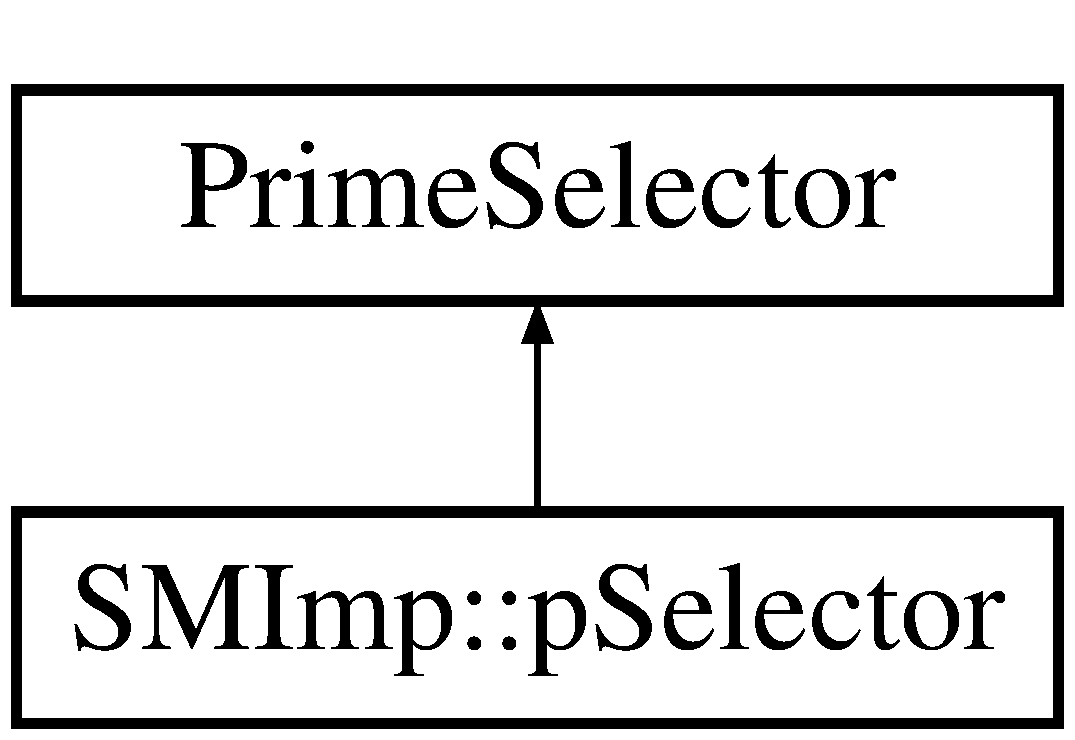
\includegraphics[height=2.000000cm]{classSMImp_1_1pSelector}
\end{center}
\end{figure}
\subsection*{Public Member Functions}
\begin{DoxyCompactItemize}
\item 
\hyperlink{classSMImp_1_1pSelector_a408417e2fa93448254ea6a36c5eb0f29}{p\+Selector} ()
\item 
\hyperlink{classSMImp_1_1pSelector_a73df279b8a33d0db836ace263e60f288}{$\sim$p\+Selector} ()
\item 
void \hyperlink{classSMImp_1_1pSelector_a095412eb63d8e76b6bb3e93cf139ead0}{setP} (Integer newp)
\item 
bool \hyperlink{classSMImp_1_1pSelector_a69d398cbd115e04490ce9fce5c8e2531}{Is\+Acceptable} (const Integer \&candidate) const
\end{DoxyCompactItemize}


\subsection{Detailed Description}
Required for selecting primes. 

\begin{DoxySeeAlso}{See also}
\hyperlink{classSMImp_1_1UtilityCompany_adeb454bff89a79e454d433bc1ccd448e}{S\+M\+Imp\+::\+Utility\+Company\+::generate\+Key()} 
\end{DoxySeeAlso}


Definition at line 117 of file examples.\+h.



\subsection{Constructor \& Destructor Documentation}
\mbox{\Hypertarget{classSMImp_1_1pSelector_a408417e2fa93448254ea6a36c5eb0f29}\label{classSMImp_1_1pSelector_a408417e2fa93448254ea6a36c5eb0f29}} 
\index{S\+M\+Imp\+::p\+Selector@{S\+M\+Imp\+::p\+Selector}!p\+Selector@{p\+Selector}}
\index{p\+Selector@{p\+Selector}!S\+M\+Imp\+::p\+Selector@{S\+M\+Imp\+::p\+Selector}}
\subsubsection{\texorpdfstring{p\+Selector()}{pSelector()}}
{\footnotesize\ttfamily S\+M\+Imp\+::p\+Selector\+::p\+Selector (\begin{DoxyParamCaption}{ }\end{DoxyParamCaption})\hspace{0.3cm}{\ttfamily [inline]}}



Definition at line 123 of file examples.\+h.

\mbox{\Hypertarget{classSMImp_1_1pSelector_a73df279b8a33d0db836ace263e60f288}\label{classSMImp_1_1pSelector_a73df279b8a33d0db836ace263e60f288}} 
\index{S\+M\+Imp\+::p\+Selector@{S\+M\+Imp\+::p\+Selector}!````~p\+Selector@{$\sim$p\+Selector}}
\index{````~p\+Selector@{$\sim$p\+Selector}!S\+M\+Imp\+::p\+Selector@{S\+M\+Imp\+::p\+Selector}}
\subsubsection{\texorpdfstring{$\sim$p\+Selector()}{~pSelector()}}
{\footnotesize\ttfamily S\+M\+Imp\+::p\+Selector\+::$\sim$p\+Selector (\begin{DoxyParamCaption}{ }\end{DoxyParamCaption})\hspace{0.3cm}{\ttfamily [inline]}}



Definition at line 127 of file examples.\+h.



\subsection{Member Function Documentation}
\mbox{\Hypertarget{classSMImp_1_1pSelector_a69d398cbd115e04490ce9fce5c8e2531}\label{classSMImp_1_1pSelector_a69d398cbd115e04490ce9fce5c8e2531}} 
\index{S\+M\+Imp\+::p\+Selector@{S\+M\+Imp\+::p\+Selector}!Is\+Acceptable@{Is\+Acceptable}}
\index{Is\+Acceptable@{Is\+Acceptable}!S\+M\+Imp\+::p\+Selector@{S\+M\+Imp\+::p\+Selector}}
\subsubsection{\texorpdfstring{Is\+Acceptable()}{IsAcceptable()}}
{\footnotesize\ttfamily bool S\+M\+Imp\+::p\+Selector\+::\+Is\+Acceptable (\begin{DoxyParamCaption}\item[{const Integer \&}]{candidate }\end{DoxyParamCaption}) const\hspace{0.3cm}{\ttfamily [inline]}}



Definition at line 135 of file examples.\+h.



References S\+M\+Imp\+::\+H\+M\+A\+C\+Payload\+::c1, S\+M\+Imp\+::\+H\+M\+A\+C\+Payload\+::c2, S\+M\+Imp\+::\+H\+M\+A\+C\+Payload\+::id, and S\+M\+Imp\+::\+H\+M\+A\+C\+Payload\+::time\+Stamp.

\mbox{\Hypertarget{classSMImp_1_1pSelector_a095412eb63d8e76b6bb3e93cf139ead0}\label{classSMImp_1_1pSelector_a095412eb63d8e76b6bb3e93cf139ead0}} 
\index{S\+M\+Imp\+::p\+Selector@{S\+M\+Imp\+::p\+Selector}!setP@{setP}}
\index{setP@{setP}!S\+M\+Imp\+::p\+Selector@{S\+M\+Imp\+::p\+Selector}}
\subsubsection{\texorpdfstring{set\+P()}{setP()}}
{\footnotesize\ttfamily void S\+M\+Imp\+::p\+Selector\+::setP (\begin{DoxyParamCaption}\item[{Integer}]{newp }\end{DoxyParamCaption})\hspace{0.3cm}{\ttfamily [inline]}}



Definition at line 130 of file examples.\+h.



The documentation for this class was generated from the following file\+:\begin{DoxyCompactItemize}
\item 
src/crypto/\hyperlink{examples_8h}{examples.\+h}\end{DoxyCompactItemize}

\hypertarget{classSMImp_1_1Requester}{}\section{S\+M\+Imp\+:\+:Requester Class Reference}
\label{classSMImp_1_1Requester}\index{S\+M\+Imp\+::\+Requester@{S\+M\+Imp\+::\+Requester}}


Abstract \hyperlink{classSMImp_1_1Requester}{Requester} Class.  




{\ttfamily \#include $<$Requester.\+h$>$}

Inheritance diagram for S\+M\+Imp\+:\+:Requester\+:\begin{figure}[H]
\begin{center}
\leavevmode
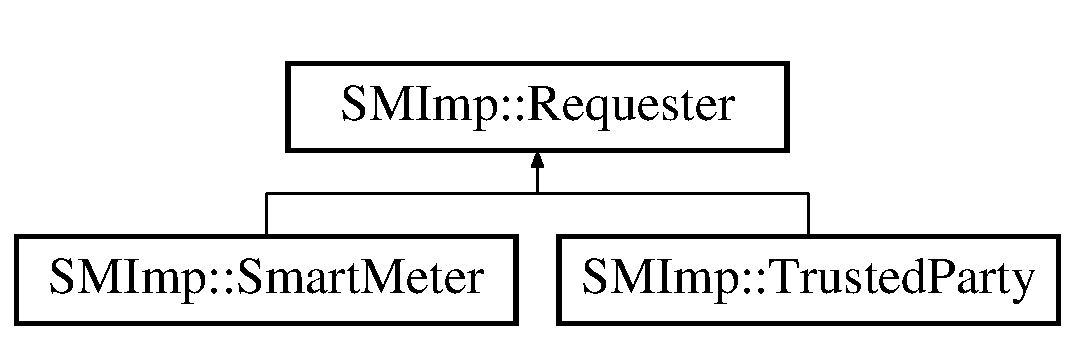
\includegraphics[height=2.000000cm]{classSMImp_1_1Requester}
\end{center}
\end{figure}
\subsection*{Public Member Functions}
\begin{DoxyCompactItemize}
\item 
bool \hyperlink{classSMImp_1_1Requester_aeba5d66cc755813cf8a7ae07c6800afe}{get\+Partials} (Integer, \hyperlink{structSMImp_1_1Payload}{Payload})
\item 
\hyperlink{classSMImp_1_1Requester_a4744d2fc0acb30a3ddfeac5d5d260e5e}{Requester} (Integer, S\+H\+A1 $\ast$)
\item 
\hyperlink{classSMImp_1_1Requester_afa51c29da77f8040ab34da85604e043d}{Requester} (Integer)
\item 
\hyperlink{classSMImp_1_1Requester_a2ba23cedf593171733290231dd4147c9}{$\sim$\+Requester} ()
\item 
Integer \hyperlink{classSMImp_1_1Requester_aab47f28abff18bff606b09a6f08b777f}{get\+Id} ()
\item 
bool \hyperlink{classSMImp_1_1Requester_ab284de7cb9eb32ae06d4f4359023d82b}{generate\+Keys} (\hyperlink{structSMImp_1_1Payload}{Payload})
\item 
\hyperlink{structSMImp_1_1Key}{Key} \hyperlink{classSMImp_1_1Requester_a02db2b7bd3da670640cc382da7100653}{get\+Public\+Key} ()
\item 
Integer \hyperlink{classSMImp_1_1Requester_a1aaa8a7e923b59ddf07b97d0f68a7fba}{get\+Public\+Partial} ()
\item 
Integer \hyperlink{classSMImp_1_1Requester_ae2056dddfa3eebd8a84ed407038ec064}{get\+Public\+Mu} ()
\end{DoxyCompactItemize}
\subsection*{Data Fields}
\begin{DoxyCompactItemize}
\item 
\hyperlink{structSMImp_1_1KeyPair}{Key\+Pair} \hyperlink{classSMImp_1_1Requester_a9203ce4677233f2dba858b5b6ec2d8be}{keys}
\begin{DoxyCompactList}\small\item\em Public and private keys. \end{DoxyCompactList}\item 
\hyperlink{structSMImp_1_1MasterKey}{Master\+Key} \hyperlink{classSMImp_1_1Requester_a140f38a7e3106bf0df39eb6370fca2f0}{params}
\begin{DoxyCompactList}\small\item\em Collection of parameters used for key generation. \end{DoxyCompactList}\item 
Nonblocking\+Rng $\ast$ \hyperlink{classSMImp_1_1Requester_aafd8f13c137f7372eda2e4f781048402}{rng}
\begin{DoxyCompactList}\small\item\em Nonblocking\+Rng Random Number Generator for key generation. \end{DoxyCompactList}\item 
Integer \hyperlink{classSMImp_1_1Requester_a16911083f2e3fc903ed3e6e7ca2a58b1}{id}
\begin{DoxyCompactList}\small\item\em ID of the particular device, used for key generation. \end{DoxyCompactList}\item 
S\+H\+A1 $\ast$ \hyperlink{classSMImp_1_1Requester_aab1bd0f1a383b17cad9e2621c2650411}{shaone}
\begin{DoxyCompactList}\small\item\em Crypto\+P\+P\+::\+S\+H\+A1 generator class. \end{DoxyCompactList}\item 
Integer \hyperlink{classSMImp_1_1Requester_a2acc3ab496a01ff90429b95d6af6ef32}{mu}
\begin{DoxyCompactList}\small\item\em Generated key segment. \end{DoxyCompactList}\item 
Integer \hyperlink{classSMImp_1_1Requester_ac5f95176425aabf5fa3fb4bb8d152167}{R}
\begin{DoxyCompactList}\small\item\em Shared-\/secrete R. \end{DoxyCompactList}\item 
Integer \hyperlink{classSMImp_1_1Requester_a95d364e3698162c3d3f2502da572bc23}{session\+Key}
\begin{DoxyCompactList}\small\item\em Shared session key. \end{DoxyCompactList}\end{DoxyCompactItemize}


\subsection{Detailed Description}
Abstract \hyperlink{classSMImp_1_1Requester}{Requester} Class. 

Intended to be extended by any object which utiizes Diffie–\+Hellman key exchange 

Definition at line 12 of file Requester.\+h.



\subsection{Constructor \& Destructor Documentation}
\mbox{\Hypertarget{classSMImp_1_1Requester_a4744d2fc0acb30a3ddfeac5d5d260e5e}\label{classSMImp_1_1Requester_a4744d2fc0acb30a3ddfeac5d5d260e5e}} 
\index{S\+M\+Imp\+::\+Requester@{S\+M\+Imp\+::\+Requester}!Requester@{Requester}}
\index{Requester@{Requester}!S\+M\+Imp\+::\+Requester@{S\+M\+Imp\+::\+Requester}}
\subsubsection{\texorpdfstring{Requester()}{Requester()}\hspace{0.1cm}{\footnotesize\ttfamily [1/2]}}
{\footnotesize\ttfamily S\+M\+Imp\+::\+Requester\+::\+Requester (\begin{DoxyParamCaption}\item[{Integer}]{i,  }\item[{S\+H\+A1 $\ast$}]{s }\end{DoxyParamCaption})}

Calls init. \begin{DoxySeeAlso}{See also}
init(\+Integer i, S\+H\+A1$\ast$ s) 
\end{DoxySeeAlso}


Definition at line 12 of file Requester.\+cc.

\mbox{\Hypertarget{classSMImp_1_1Requester_afa51c29da77f8040ab34da85604e043d}\label{classSMImp_1_1Requester_afa51c29da77f8040ab34da85604e043d}} 
\index{S\+M\+Imp\+::\+Requester@{S\+M\+Imp\+::\+Requester}!Requester@{Requester}}
\index{Requester@{Requester}!S\+M\+Imp\+::\+Requester@{S\+M\+Imp\+::\+Requester}}
\subsubsection{\texorpdfstring{Requester()}{Requester()}\hspace{0.1cm}{\footnotesize\ttfamily [2/2]}}
{\footnotesize\ttfamily S\+M\+Imp\+::\+Requester\+::\+Requester (\begin{DoxyParamCaption}\item[{Integer}]{i }\end{DoxyParamCaption})}

Calls init. Initilizes new S\+H\+A1 class since one isn\textquotesingle{}t provided. \begin{DoxySeeAlso}{See also}
init(\+Integer i, S\+H\+A1$\ast$ s) 
\end{DoxySeeAlso}


Definition at line 6 of file Requester.\+cc.



References shaone.

\mbox{\Hypertarget{classSMImp_1_1Requester_a2ba23cedf593171733290231dd4147c9}\label{classSMImp_1_1Requester_a2ba23cedf593171733290231dd4147c9}} 
\index{S\+M\+Imp\+::\+Requester@{S\+M\+Imp\+::\+Requester}!````~Requester@{$\sim$\+Requester}}
\index{````~Requester@{$\sim$\+Requester}!S\+M\+Imp\+::\+Requester@{S\+M\+Imp\+::\+Requester}}
\subsubsection{\texorpdfstring{$\sim$\+Requester()}{~Requester()}}
{\footnotesize\ttfamily S\+M\+Imp\+::\+Requester\+::$\sim$\+Requester (\begin{DoxyParamCaption}{ }\end{DoxyParamCaption})}



Definition at line 17 of file Requester.\+cc.



References rng, and shaone.



\subsection{Member Function Documentation}
\mbox{\Hypertarget{classSMImp_1_1Requester_ab284de7cb9eb32ae06d4f4359023d82b}\label{classSMImp_1_1Requester_ab284de7cb9eb32ae06d4f4359023d82b}} 
\index{S\+M\+Imp\+::\+Requester@{S\+M\+Imp\+::\+Requester}!generate\+Keys@{generate\+Keys}}
\index{generate\+Keys@{generate\+Keys}!S\+M\+Imp\+::\+Requester@{S\+M\+Imp\+::\+Requester}}
\subsubsection{\texorpdfstring{generate\+Keys()}{generateKeys()}}
{\footnotesize\ttfamily bool S\+M\+Imp\+::\+Requester\+::generate\+Keys (\begin{DoxyParamCaption}\item[{\hyperlink{structSMImp_1_1Payload}{Payload}}]{pl }\end{DoxyParamCaption})}

Generates keys from given key component payload from Utility Comapny 

Definition at line 88 of file Requester.\+cc.



References S\+M\+Imp\+::\+Master\+Key\+::g, get\+Partials(), keys, S\+M\+Imp\+::\+Master\+Key\+::p, params, S\+M\+Imp\+::\+Key\+::piece, S\+M\+Imp\+::\+Key\+Pair\+::priv, S\+M\+Imp\+::\+Key\+Pair\+::pub, S\+M\+Imp\+::\+Master\+Key\+::q, and rng.

\mbox{\Hypertarget{classSMImp_1_1Requester_aab47f28abff18bff606b09a6f08b777f}\label{classSMImp_1_1Requester_aab47f28abff18bff606b09a6f08b777f}} 
\index{S\+M\+Imp\+::\+Requester@{S\+M\+Imp\+::\+Requester}!get\+Id@{get\+Id}}
\index{get\+Id@{get\+Id}!S\+M\+Imp\+::\+Requester@{S\+M\+Imp\+::\+Requester}}
\subsubsection{\texorpdfstring{get\+Id()}{getId()}}
{\footnotesize\ttfamily Integer S\+M\+Imp\+::\+Requester\+::get\+Id (\begin{DoxyParamCaption}{ }\end{DoxyParamCaption})}

Returns ID of the Smart Meter. \begin{DoxyReturn}{Returns}
ID of the Smart Meter. 
\end{DoxyReturn}


Definition at line 43 of file Requester.\+cc.



References id.

\mbox{\Hypertarget{classSMImp_1_1Requester_aeba5d66cc755813cf8a7ae07c6800afe}\label{classSMImp_1_1Requester_aeba5d66cc755813cf8a7ae07c6800afe}} 
\index{S\+M\+Imp\+::\+Requester@{S\+M\+Imp\+::\+Requester}!get\+Partials@{get\+Partials}}
\index{get\+Partials@{get\+Partials}!S\+M\+Imp\+::\+Requester@{S\+M\+Imp\+::\+Requester}}
\subsubsection{\texorpdfstring{get\+Partials()}{getPartials()}}
{\footnotesize\ttfamily bool S\+M\+Imp\+::\+Requester\+::get\+Partials (\begin{DoxyParamCaption}\item[{Integer}]{i,  }\item[{\hyperlink{structSMImp_1_1Payload}{Payload}}]{pl }\end{DoxyParamCaption})}

function for recieving partial keys from Utility Company. 

Definition at line 48 of file Requester.\+cc.



References S\+M\+Imp\+::\+Master\+Key\+::g, keys, S\+M\+Imp\+::\+Master\+Key\+::p, params, S\+M\+Imp\+::\+Payload\+::params, S\+M\+Imp\+::\+Key\+::partial, S\+M\+Imp\+::\+Key\+Pair\+::priv, S\+M\+Imp\+::\+Payload\+::priv, S\+M\+Imp\+::\+Key\+Pair\+::pub, S\+M\+Imp\+::\+Payload\+::pub, shaone, and S\+M\+Imp\+::\+Master\+Key\+::x.

\mbox{\Hypertarget{classSMImp_1_1Requester_a02db2b7bd3da670640cc382da7100653}\label{classSMImp_1_1Requester_a02db2b7bd3da670640cc382da7100653}} 
\index{S\+M\+Imp\+::\+Requester@{S\+M\+Imp\+::\+Requester}!get\+Public\+Key@{get\+Public\+Key}}
\index{get\+Public\+Key@{get\+Public\+Key}!S\+M\+Imp\+::\+Requester@{S\+M\+Imp\+::\+Requester}}
\subsubsection{\texorpdfstring{get\+Public\+Key()}{getPublicKey()}}
{\footnotesize\ttfamily \hyperlink{structSMImp_1_1Key}{Key} S\+M\+Imp\+::\+Requester\+::get\+Public\+Key (\begin{DoxyParamCaption}{ }\end{DoxyParamCaption})}

\begin{DoxyReturn}{Returns}
Public key 
\end{DoxyReturn}


Definition at line 38 of file Requester.\+cc.



References keys, and S\+M\+Imp\+::\+Key\+Pair\+::pub.

\mbox{\Hypertarget{classSMImp_1_1Requester_ae2056dddfa3eebd8a84ed407038ec064}\label{classSMImp_1_1Requester_ae2056dddfa3eebd8a84ed407038ec064}} 
\index{S\+M\+Imp\+::\+Requester@{S\+M\+Imp\+::\+Requester}!get\+Public\+Mu@{get\+Public\+Mu}}
\index{get\+Public\+Mu@{get\+Public\+Mu}!S\+M\+Imp\+::\+Requester@{S\+M\+Imp\+::\+Requester}}
\subsubsection{\texorpdfstring{get\+Public\+Mu()}{getPublicMu()}}
{\footnotesize\ttfamily Integer S\+M\+Imp\+::\+Requester\+::get\+Public\+Mu (\begin{DoxyParamCaption}{ }\end{DoxyParamCaption})}

\begin{DoxyReturn}{Returns}
Generated piece from public key. 
\end{DoxyReturn}
\begin{DoxySeeAlso}{See also}
\hyperlink{classSMImp_1_1Requester_a1aaa8a7e923b59ddf07b97d0f68a7fba}{get\+Public\+Partial()} and \hyperlink{classSMImp_1_1Requester_a02db2b7bd3da670640cc382da7100653}{get\+Public\+Key()} 
\end{DoxySeeAlso}


Definition at line 28 of file Requester.\+cc.



References keys, S\+M\+Imp\+::\+Key\+::piece, and S\+M\+Imp\+::\+Key\+Pair\+::pub.

\mbox{\Hypertarget{classSMImp_1_1Requester_a1aaa8a7e923b59ddf07b97d0f68a7fba}\label{classSMImp_1_1Requester_a1aaa8a7e923b59ddf07b97d0f68a7fba}} 
\index{S\+M\+Imp\+::\+Requester@{S\+M\+Imp\+::\+Requester}!get\+Public\+Partial@{get\+Public\+Partial}}
\index{get\+Public\+Partial@{get\+Public\+Partial}!S\+M\+Imp\+::\+Requester@{S\+M\+Imp\+::\+Requester}}
\subsubsection{\texorpdfstring{get\+Public\+Partial()}{getPublicPartial()}}
{\footnotesize\ttfamily Integer S\+M\+Imp\+::\+Requester\+::get\+Public\+Partial (\begin{DoxyParamCaption}{ }\end{DoxyParamCaption})}

\begin{DoxyReturn}{Returns}
Partial public key (component generated by Utility Company). 
\end{DoxyReturn}


Definition at line 33 of file Requester.\+cc.



References keys, S\+M\+Imp\+::\+Key\+::partial, and S\+M\+Imp\+::\+Key\+Pair\+::pub.



\subsection{Field Documentation}
\mbox{\Hypertarget{classSMImp_1_1Requester_a16911083f2e3fc903ed3e6e7ca2a58b1}\label{classSMImp_1_1Requester_a16911083f2e3fc903ed3e6e7ca2a58b1}} 
\index{S\+M\+Imp\+::\+Requester@{S\+M\+Imp\+::\+Requester}!id@{id}}
\index{id@{id}!S\+M\+Imp\+::\+Requester@{S\+M\+Imp\+::\+Requester}}
\subsubsection{\texorpdfstring{id}{id}}
{\footnotesize\ttfamily Integer S\+M\+Imp\+::\+Requester\+::id}



ID of the particular device, used for key generation. 



Definition at line 31 of file Requester.\+h.

\mbox{\Hypertarget{classSMImp_1_1Requester_a9203ce4677233f2dba858b5b6ec2d8be}\label{classSMImp_1_1Requester_a9203ce4677233f2dba858b5b6ec2d8be}} 
\index{S\+M\+Imp\+::\+Requester@{S\+M\+Imp\+::\+Requester}!keys@{keys}}
\index{keys@{keys}!S\+M\+Imp\+::\+Requester@{S\+M\+Imp\+::\+Requester}}
\subsubsection{\texorpdfstring{keys}{keys}}
{\footnotesize\ttfamily \hyperlink{structSMImp_1_1KeyPair}{Key\+Pair} S\+M\+Imp\+::\+Requester\+::keys}



Public and private keys. 



Definition at line 25 of file Requester.\+h.

\mbox{\Hypertarget{classSMImp_1_1Requester_a2acc3ab496a01ff90429b95d6af6ef32}\label{classSMImp_1_1Requester_a2acc3ab496a01ff90429b95d6af6ef32}} 
\index{S\+M\+Imp\+::\+Requester@{S\+M\+Imp\+::\+Requester}!mu@{mu}}
\index{mu@{mu}!S\+M\+Imp\+::\+Requester@{S\+M\+Imp\+::\+Requester}}
\subsubsection{\texorpdfstring{mu}{mu}}
{\footnotesize\ttfamily Integer S\+M\+Imp\+::\+Requester\+::mu}



Generated key segment. 



Definition at line 36 of file Requester.\+h.

\mbox{\Hypertarget{classSMImp_1_1Requester_a140f38a7e3106bf0df39eb6370fca2f0}\label{classSMImp_1_1Requester_a140f38a7e3106bf0df39eb6370fca2f0}} 
\index{S\+M\+Imp\+::\+Requester@{S\+M\+Imp\+::\+Requester}!params@{params}}
\index{params@{params}!S\+M\+Imp\+::\+Requester@{S\+M\+Imp\+::\+Requester}}
\subsubsection{\texorpdfstring{params}{params}}
{\footnotesize\ttfamily \hyperlink{structSMImp_1_1MasterKey}{Master\+Key} S\+M\+Imp\+::\+Requester\+::params}



Collection of parameters used for key generation. 



Definition at line 27 of file Requester.\+h.

\mbox{\Hypertarget{classSMImp_1_1Requester_ac5f95176425aabf5fa3fb4bb8d152167}\label{classSMImp_1_1Requester_ac5f95176425aabf5fa3fb4bb8d152167}} 
\index{S\+M\+Imp\+::\+Requester@{S\+M\+Imp\+::\+Requester}!R@{R}}
\index{R@{R}!S\+M\+Imp\+::\+Requester@{S\+M\+Imp\+::\+Requester}}
\subsubsection{\texorpdfstring{R}{R}}
{\footnotesize\ttfamily Integer S\+M\+Imp\+::\+Requester\+::R}



Shared-\/secrete R. 



Definition at line 38 of file Requester.\+h.

\mbox{\Hypertarget{classSMImp_1_1Requester_aafd8f13c137f7372eda2e4f781048402}\label{classSMImp_1_1Requester_aafd8f13c137f7372eda2e4f781048402}} 
\index{S\+M\+Imp\+::\+Requester@{S\+M\+Imp\+::\+Requester}!rng@{rng}}
\index{rng@{rng}!S\+M\+Imp\+::\+Requester@{S\+M\+Imp\+::\+Requester}}
\subsubsection{\texorpdfstring{rng}{rng}}
{\footnotesize\ttfamily Nonblocking\+Rng$\ast$ S\+M\+Imp\+::\+Requester\+::rng}



Nonblocking\+Rng Random Number Generator for key generation. 



Definition at line 29 of file Requester.\+h.

\mbox{\Hypertarget{classSMImp_1_1Requester_a95d364e3698162c3d3f2502da572bc23}\label{classSMImp_1_1Requester_a95d364e3698162c3d3f2502da572bc23}} 
\index{S\+M\+Imp\+::\+Requester@{S\+M\+Imp\+::\+Requester}!session\+Key@{session\+Key}}
\index{session\+Key@{session\+Key}!S\+M\+Imp\+::\+Requester@{S\+M\+Imp\+::\+Requester}}
\subsubsection{\texorpdfstring{session\+Key}{sessionKey}}
{\footnotesize\ttfamily Integer S\+M\+Imp\+::\+Requester\+::session\+Key}



Shared session key. 



Definition at line 40 of file Requester.\+h.

\mbox{\Hypertarget{classSMImp_1_1Requester_aab1bd0f1a383b17cad9e2621c2650411}\label{classSMImp_1_1Requester_aab1bd0f1a383b17cad9e2621c2650411}} 
\index{S\+M\+Imp\+::\+Requester@{S\+M\+Imp\+::\+Requester}!shaone@{shaone}}
\index{shaone@{shaone}!S\+M\+Imp\+::\+Requester@{S\+M\+Imp\+::\+Requester}}
\subsubsection{\texorpdfstring{shaone}{shaone}}
{\footnotesize\ttfamily S\+H\+A1$\ast$ S\+M\+Imp\+::\+Requester\+::shaone}



Crypto\+P\+P\+::\+S\+H\+A1 generator class. 



Definition at line 33 of file Requester.\+h.



The documentation for this class was generated from the following files\+:\begin{DoxyCompactItemize}
\item 
src/crypto/\hyperlink{Requester_8h}{Requester.\+h}\item 
src/crypto/\hyperlink{Requester_8cc}{Requester.\+cc}\end{DoxyCompactItemize}

\hypertarget{classSMAdapter}{}\section{S\+M\+Adapter Class Reference}
\label{classSMAdapter}\index{S\+M\+Adapter@{S\+M\+Adapter}}


Smart Meter \hyperlink{classAdapter}{Adapter}.  




{\ttfamily \#include $<$S\+M\+Adapter.\+h$>$}

Inheritance diagram for S\+M\+Adapter\+:\begin{figure}[H]
\begin{center}
\leavevmode
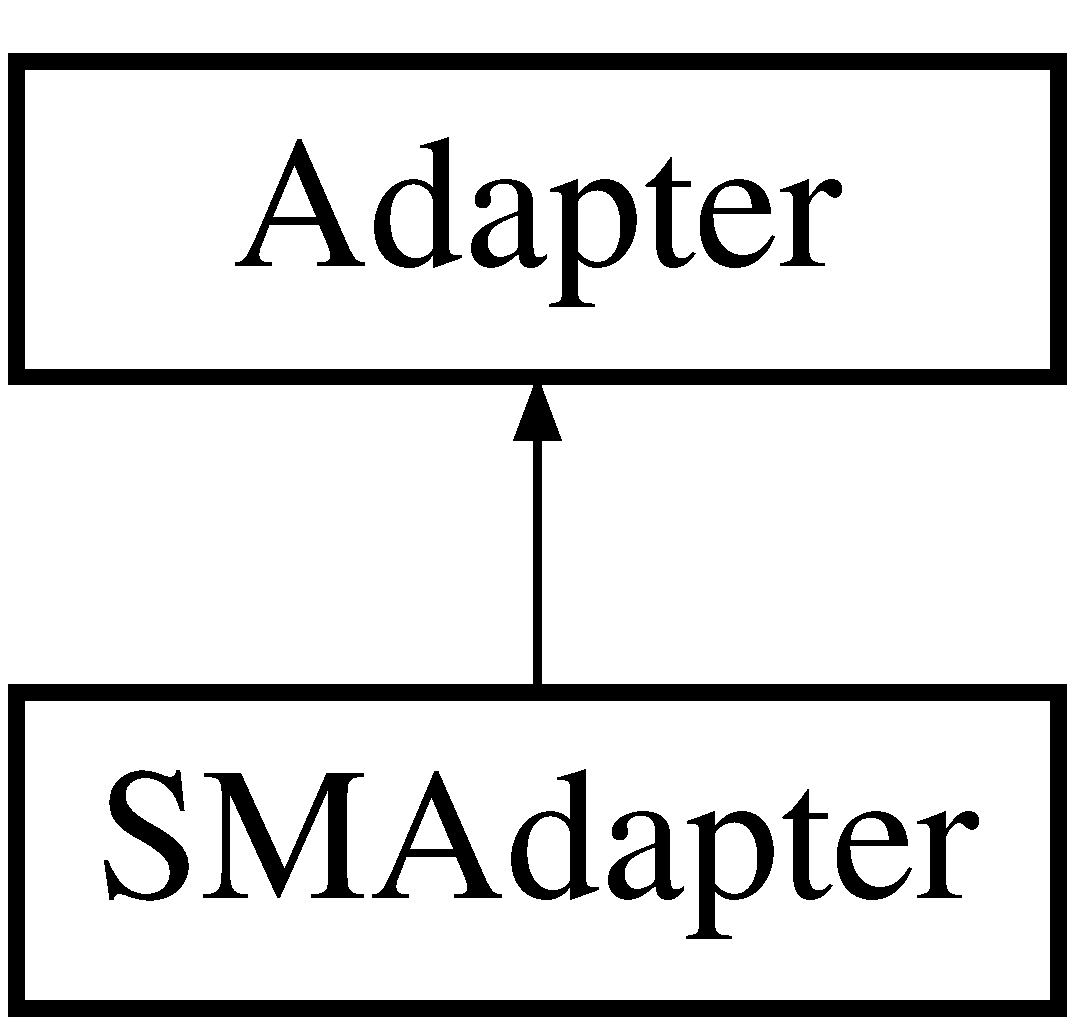
\includegraphics[height=2.000000cm]{classSMAdapter}
\end{center}
\end{figure}
\subsection*{Public Member Functions}
\begin{DoxyCompactItemize}
\item 
\hyperlink{classSMAdapter_a5bf9ca331e0f7aac7c182ef080ef74eb}{S\+M\+Adapter} (long int i)
\item 
\hyperlink{classSMAdapter_a4f8ec3739e23b40a4b4c3c26490d1c27}{S\+M\+Adapter} (long int i, \hyperlink{classsmart3p_1_1Unit}{smart3p\+::\+Unit} $\ast$u)
\item 
\hyperlink{classSMAdapter_a935746ba8f7210132ac6324efba1c210}{$\sim$\+S\+M\+Adapter} ()
\item 
void \hyperlink{classSMAdapter_ad35493a50872a683b4b5e0671f783769}{register\+Info\+From\+UC} (omnetpp\+::c\+Message $\ast$msg)
\item 
\hyperlink{classcInteger}{c\+Integer} $\ast$ \hyperlink{classSMAdapter_a3568d35fe2de8828cb6fcaf0bd9d9923}{get\+Id} ()
\item 
\hyperlink{classcInteger}{c\+Integer} $\ast$ \hyperlink{classSMAdapter_a586f83c19527bf0401a50424c24eece1}{get\+Anon\+Id} ()
\item 
omnetpp\+::c\+Queue $\ast$ \hyperlink{classSMAdapter_ab4ec874f14fd50ad8c5fc50c500981c4}{start\+Session\+Key\+Exchange} (omnetpp\+::c\+Message $\ast$msg)
\item 
bool \hyperlink{classSMAdapter_adcce474ffc3ad9717b3307ac95fa1445}{end\+Of\+Session\+Key\+Exchange} (omnetpp\+::c\+Message $\ast$msg)
\item 
omnetpp\+::c\+Message $\ast$ \hyperlink{classSMAdapter_a9e36c5113b54f4b1a2a9f0c3fac4dd22}{send\+Energy\+Consumption} (omnetpp\+::c\+Message $\ast$msg)
\item 
void \hyperlink{classSMAdapter_aecfd03fc0facc3c1a9b43cedce2d026a}{log} (char $\ast$, double)
\item 
void \hyperlink{classSMAdapter_a695f8eb90b349dc6267eb82ec9f9ee93}{add\+Sim\+Time} (double)
\end{DoxyCompactItemize}
\subsection*{Additional Inherited Members}


\subsection{Detailed Description}
Smart Meter \hyperlink{classAdapter}{Adapter}. 

Definition at line 15 of file S\+M\+Adapter.\+h.



\subsection{Constructor \& Destructor Documentation}
\mbox{\Hypertarget{classSMAdapter_a5bf9ca331e0f7aac7c182ef080ef74eb}\label{classSMAdapter_a5bf9ca331e0f7aac7c182ef080ef74eb}} 
\index{S\+M\+Adapter@{S\+M\+Adapter}!S\+M\+Adapter@{S\+M\+Adapter}}
\index{S\+M\+Adapter@{S\+M\+Adapter}!S\+M\+Adapter@{S\+M\+Adapter}}
\subsubsection{\texorpdfstring{S\+M\+Adapter()}{SMAdapter()}\hspace{0.1cm}{\footnotesize\ttfamily [1/2]}}
{\footnotesize\ttfamily S\+M\+Adapter\+::\+S\+M\+Adapter (\begin{DoxyParamCaption}\item[{long int}]{i }\end{DoxyParamCaption})}


\begin{DoxyParams}{Parameters}
{\em i} & Smart Meter ID \\
\hline
\end{DoxyParams}


Definition at line 16 of file S\+M\+Adapter.\+cc.

\mbox{\Hypertarget{classSMAdapter_a4f8ec3739e23b40a4b4c3c26490d1c27}\label{classSMAdapter_a4f8ec3739e23b40a4b4c3c26490d1c27}} 
\index{S\+M\+Adapter@{S\+M\+Adapter}!S\+M\+Adapter@{S\+M\+Adapter}}
\index{S\+M\+Adapter@{S\+M\+Adapter}!S\+M\+Adapter@{S\+M\+Adapter}}
\subsubsection{\texorpdfstring{S\+M\+Adapter()}{SMAdapter()}\hspace{0.1cm}{\footnotesize\ttfamily [2/2]}}
{\footnotesize\ttfamily S\+M\+Adapter\+::\+S\+M\+Adapter (\begin{DoxyParamCaption}\item[{long int}]{i,  }\item[{\hyperlink{classsmart3p_1_1Unit}{smart3p\+::\+Unit} $\ast$}]{u }\end{DoxyParamCaption})}


\begin{DoxyParams}{Parameters}
{\em i} & Smart Meter ID \\
\hline
{\em u} & Output unit class (used for debugging) \\
\hline
\end{DoxyParams}
\begin{DoxySeeAlso}{See also}
\hyperlink{classSMAdapter_aecfd03fc0facc3c1a9b43cedce2d026a}{log(char$\ast$, double)}, \hyperlink{classSMAdapter_a695f8eb90b349dc6267eb82ec9f9ee93}{add\+Sim\+Time(double)} 
\end{DoxySeeAlso}


Definition at line 21 of file S\+M\+Adapter.\+cc.

\mbox{\Hypertarget{classSMAdapter_a935746ba8f7210132ac6324efba1c210}\label{classSMAdapter_a935746ba8f7210132ac6324efba1c210}} 
\index{S\+M\+Adapter@{S\+M\+Adapter}!````~S\+M\+Adapter@{$\sim$\+S\+M\+Adapter}}
\index{````~S\+M\+Adapter@{$\sim$\+S\+M\+Adapter}!S\+M\+Adapter@{S\+M\+Adapter}}
\subsubsection{\texorpdfstring{$\sim$\+S\+M\+Adapter()}{~SMAdapter()}}
{\footnotesize\ttfamily S\+M\+Adapter\+::$\sim$\+S\+M\+Adapter (\begin{DoxyParamCaption}{ }\end{DoxyParamCaption})}



Definition at line 26 of file S\+M\+Adapter.\+cc.



\subsection{Member Function Documentation}
\mbox{\Hypertarget{classSMAdapter_a695f8eb90b349dc6267eb82ec9f9ee93}\label{classSMAdapter_a695f8eb90b349dc6267eb82ec9f9ee93}} 
\index{S\+M\+Adapter@{S\+M\+Adapter}!add\+Sim\+Time@{add\+Sim\+Time}}
\index{add\+Sim\+Time@{add\+Sim\+Time}!S\+M\+Adapter@{S\+M\+Adapter}}
\subsubsection{\texorpdfstring{add\+Sim\+Time()}{addSimTime()}}
{\footnotesize\ttfamily void S\+M\+Adapter\+::add\+Sim\+Time (\begin{DoxyParamCaption}\item[{double}]{time }\end{DoxyParamCaption})}

Adds time to the simulation 

Definition at line 31 of file S\+M\+Adapter.\+cc.



References Adapter\+::out.

\mbox{\Hypertarget{classSMAdapter_adcce474ffc3ad9717b3307ac95fa1445}\label{classSMAdapter_adcce474ffc3ad9717b3307ac95fa1445}} 
\index{S\+M\+Adapter@{S\+M\+Adapter}!end\+Of\+Session\+Key\+Exchange@{end\+Of\+Session\+Key\+Exchange}}
\index{end\+Of\+Session\+Key\+Exchange@{end\+Of\+Session\+Key\+Exchange}!S\+M\+Adapter@{S\+M\+Adapter}}
\subsubsection{\texorpdfstring{end\+Of\+Session\+Key\+Exchange()}{endOfSessionKeyExchange()}}
{\footnotesize\ttfamily bool S\+M\+Adapter\+::end\+Of\+Session\+Key\+Exchange (\begin{DoxyParamCaption}\item[{omnetpp\+::c\+Message $\ast$}]{msg }\end{DoxyParamCaption})}

Finishes the session key exchange phase. \begin{DoxyReturn}{Returns}
tells if the final session key passed verification. 
\end{DoxyReturn}


Definition at line 155 of file S\+M\+Adapter.\+cc.



References S\+M\+Imp\+::\+Smart\+Meter\+::recieve\+H\+M\+A\+C().

\mbox{\Hypertarget{classSMAdapter_a586f83c19527bf0401a50424c24eece1}\label{classSMAdapter_a586f83c19527bf0401a50424c24eece1}} 
\index{S\+M\+Adapter@{S\+M\+Adapter}!get\+Anon\+Id@{get\+Anon\+Id}}
\index{get\+Anon\+Id@{get\+Anon\+Id}!S\+M\+Adapter@{S\+M\+Adapter}}
\subsubsection{\texorpdfstring{get\+Anon\+Id()}{getAnonId()}}
{\footnotesize\ttfamily \hyperlink{classcInteger}{c\+Integer} $\ast$ S\+M\+Adapter\+::get\+Anon\+Id (\begin{DoxyParamCaption}{ }\end{DoxyParamCaption})}

Gets the Anonymous ID from the underlying protocol Smart Meter 

Definition at line 42 of file S\+M\+Adapter.\+cc.



References S\+M\+Imp\+::\+Smart\+Meter\+::get\+Anon\+Id().

\mbox{\Hypertarget{classSMAdapter_a3568d35fe2de8828cb6fcaf0bd9d9923}\label{classSMAdapter_a3568d35fe2de8828cb6fcaf0bd9d9923}} 
\index{S\+M\+Adapter@{S\+M\+Adapter}!get\+Id@{get\+Id}}
\index{get\+Id@{get\+Id}!S\+M\+Adapter@{S\+M\+Adapter}}
\subsubsection{\texorpdfstring{get\+Id()}{getId()}}
{\footnotesize\ttfamily \hyperlink{classcInteger}{c\+Integer} $\ast$ S\+M\+Adapter\+::get\+Id (\begin{DoxyParamCaption}{ }\end{DoxyParamCaption})}

Gets the ID from the underlying protocol Smart Meter 

Definition at line 47 of file S\+M\+Adapter.\+cc.



References S\+M\+Imp\+::\+Requester\+::get\+Id().

\mbox{\Hypertarget{classSMAdapter_aecfd03fc0facc3c1a9b43cedce2d026a}\label{classSMAdapter_aecfd03fc0facc3c1a9b43cedce2d026a}} 
\index{S\+M\+Adapter@{S\+M\+Adapter}!log@{log}}
\index{log@{log}!S\+M\+Adapter@{S\+M\+Adapter}}
\subsubsection{\texorpdfstring{log()}{log()}}
{\footnotesize\ttfamily void S\+M\+Adapter\+::log (\begin{DoxyParamCaption}\item[{char $\ast$}]{tag,  }\item[{double}]{value }\end{DoxyParamCaption})}

Emits statistical data. 

Definition at line 36 of file S\+M\+Adapter.\+cc.



References Adapter\+::out.

\mbox{\Hypertarget{classSMAdapter_ad35493a50872a683b4b5e0671f783769}\label{classSMAdapter_ad35493a50872a683b4b5e0671f783769}} 
\index{S\+M\+Adapter@{S\+M\+Adapter}!register\+Info\+From\+UC@{register\+Info\+From\+UC}}
\index{register\+Info\+From\+UC@{register\+Info\+From\+UC}!S\+M\+Adapter@{S\+M\+Adapter}}
\subsubsection{\texorpdfstring{register\+Info\+From\+U\+C()}{registerInfoFromUC()}}
{\footnotesize\ttfamily void S\+M\+Adapter\+::register\+Info\+From\+UC (\begin{DoxyParamCaption}\item[{omnetpp\+::c\+Message $\ast$}]{msg }\end{DoxyParamCaption})}

Registers key data from Utility Company. 

Definition at line 52 of file S\+M\+Adapter.\+cc.



References S\+M\+Imp\+::\+Master\+Key\+::g, S\+M\+Imp\+::\+Smart\+Meter\+::generate\+Keys(), S\+M\+Imp\+::\+Master\+Key\+::p, S\+M\+Imp\+::\+Payload\+::params, Adapter\+::print(), S\+M\+Imp\+::\+Payload\+::priv, S\+M\+Imp\+::\+Payload\+::pub, S\+M\+Imp\+::\+Master\+Key\+::q, S\+M\+Imp\+::\+Smart\+Meter\+::set\+Anon\+Id(), S\+M\+Imp\+::\+Smart\+Meter\+::set\+H\+M\+A\+C\+Key(), Adapter\+::verbose, and S\+M\+Imp\+::\+Master\+Key\+::x.

\mbox{\Hypertarget{classSMAdapter_a9e36c5113b54f4b1a2a9f0c3fac4dd22}\label{classSMAdapter_a9e36c5113b54f4b1a2a9f0c3fac4dd22}} 
\index{S\+M\+Adapter@{S\+M\+Adapter}!send\+Energy\+Consumption@{send\+Energy\+Consumption}}
\index{send\+Energy\+Consumption@{send\+Energy\+Consumption}!S\+M\+Adapter@{S\+M\+Adapter}}
\subsubsection{\texorpdfstring{send\+Energy\+Consumption()}{sendEnergyConsumption()}}
{\footnotesize\ttfamily omnetpp\+::c\+Message $\ast$ S\+M\+Adapter\+::send\+Energy\+Consumption (\begin{DoxyParamCaption}\item[{omnetpp\+::c\+Message $\ast$}]{msg }\end{DoxyParamCaption})}

Sends encrypted energy use data to Trusted Thrid Party. 

Definition at line 166 of file S\+M\+Adapter.\+cc.



References S\+M\+Imp\+::\+H\+M\+A\+C\+Payload\+::c1, S\+M\+Imp\+::\+H\+M\+A\+C\+Payload\+::c2, smart3p\+::\+S\+M\+Packet\+::get\+Value(), S\+M\+Imp\+::\+H\+M\+A\+C\+Payload\+::hmac, S\+M\+Imp\+::\+H\+M\+A\+C\+Payload\+::id, S\+M\+Imp\+::\+H\+M\+A\+C\+Payload\+::message\+Length, S\+M\+Imp\+::\+Packet\+::pl, Adapter\+::print(), S\+M\+Imp\+::\+Smart\+Meter\+::send\+Data\+To\+T\+T\+P(), S\+M\+Imp\+::\+H\+M\+A\+C\+Payload\+::time\+Stamp, and Adapter\+::verbose.

\mbox{\Hypertarget{classSMAdapter_ab4ec874f14fd50ad8c5fc50c500981c4}\label{classSMAdapter_ab4ec874f14fd50ad8c5fc50c500981c4}} 
\index{S\+M\+Adapter@{S\+M\+Adapter}!start\+Session\+Key\+Exchange@{start\+Session\+Key\+Exchange}}
\index{start\+Session\+Key\+Exchange@{start\+Session\+Key\+Exchange}!S\+M\+Adapter@{S\+M\+Adapter}}
\subsubsection{\texorpdfstring{start\+Session\+Key\+Exchange()}{startSessionKeyExchange()}}
{\footnotesize\ttfamily omnetpp\+::c\+Queue $\ast$ S\+M\+Adapter\+::start\+Session\+Key\+Exchange (\begin{DoxyParamCaption}\item[{omnetpp\+::c\+Message $\ast$}]{msg }\end{DoxyParamCaption})}

Starts the session key generation. \begin{DoxyReturn}{Returns}
Queue of packets to be sent to Trusted Thrid Party. 
\end{DoxyReturn}


Definition at line 82 of file S\+M\+Adapter.\+cc.



References S\+M\+Imp\+::\+H\+M\+A\+C\+Payload\+::c1, S\+M\+Imp\+::\+H\+M\+A\+C\+Payload\+::c2, smart3p\+::\+S\+M\+Packet\+::get\+Id(), S\+M\+Imp\+::\+Requester\+::get\+Id(), S\+M\+Imp\+::\+Requester\+::get\+Public\+Mu(), S\+M\+Imp\+::\+Requester\+::get\+Public\+Partial(), S\+M\+Imp\+::\+H\+M\+A\+C\+Payload\+::hmac, S\+M\+Imp\+::\+H\+M\+A\+C\+Payload\+::message\+Length, S\+M\+Imp\+::\+Packet\+::pl, Adapter\+::print(), S\+M\+Imp\+::\+H\+M\+A\+C\+Payload\+::r, S\+M\+Imp\+::\+Smart\+Meter\+::session\+Key\+Exchange(), smart3p\+::\+S\+M\+Packet\+::set\+Id(), and S\+M\+Imp\+::\+H\+M\+A\+C\+Payload\+::time\+Stamp.



The documentation for this class was generated from the following files\+:\begin{DoxyCompactItemize}
\item 
src/\hyperlink{SMAdapter_8h}{S\+M\+Adapter.\+h}\item 
src/\hyperlink{SMAdapter_8cc}{S\+M\+Adapter.\+cc}\end{DoxyCompactItemize}

\hypertarget{classsmart3p_1_1SmartMeter}{}\section{smart3p\+:\+:Smart\+Meter Class Reference}
\label{classsmart3p_1_1SmartMeter}\index{smart3p\+::\+Smart\+Meter@{smart3p\+::\+Smart\+Meter}}


Simulation Smart Meter class.  




{\ttfamily \#include $<$Smart\+Meter.\+h$>$}

Inheritance diagram for smart3p\+:\+:Smart\+Meter\+:\begin{figure}[H]
\begin{center}
\leavevmode
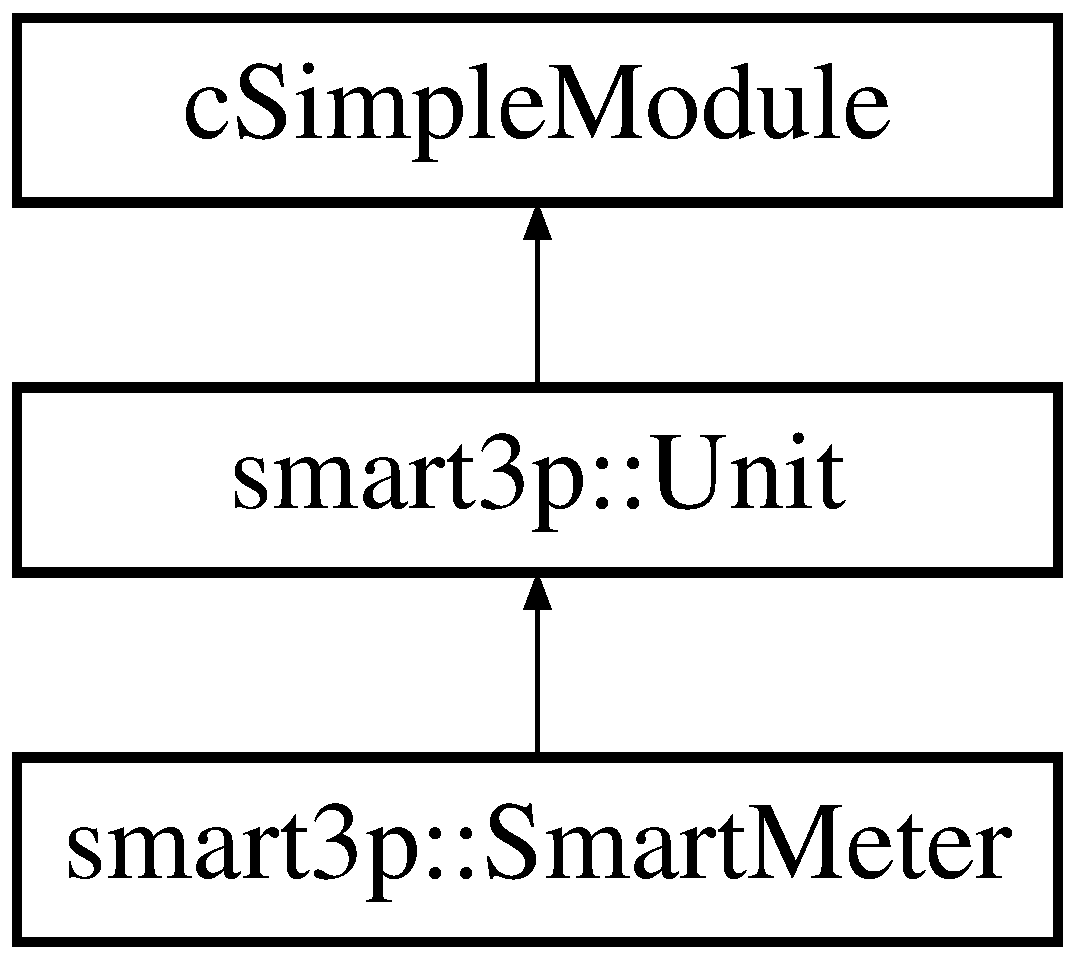
\includegraphics[height=3.000000cm]{classsmart3p_1_1SmartMeter}
\end{center}
\end{figure}
\subsection*{Public Member Functions}
\begin{DoxyCompactItemize}
\item 
void \hyperlink{classsmart3p_1_1SmartMeter_ac65e2f27b0a9d2545000baac6e1e574d}{log} (simsignal\+\_\+t id, double value)
\item 
void \hyperlink{classsmart3p_1_1SmartMeter_af92e8b7e3eaf5d1ec6e3c3f5082e8c14}{log} (char $\ast$tag, double value)
\item 
void \hyperlink{classsmart3p_1_1SmartMeter_a3b18ccd6e38a60e4e96d7e6d5b971dbe}{add\+Sim\+Time} (double t)
\end{DoxyCompactItemize}
\subsection*{Protected Member Functions}
\begin{DoxyCompactItemize}
\item 
virtual void \hyperlink{classsmart3p_1_1SmartMeter_a289d547f41c3f011e99bc0eaf5bd945b}{initialize} ()
\begin{DoxyCompactList}\small\item\em Initilizer. \end{DoxyCompactList}\item 
virtual void \hyperlink{classsmart3p_1_1SmartMeter_a3491294618643d423e8fd3578eb3a439}{timed\+Handle\+Message} (c\+Message $\ast$msg)
\begin{DoxyCompactList}\small\item\em Message Handler. \end{DoxyCompactList}\item 
virtual void \hyperlink{classsmart3p_1_1SmartMeter_a315ed406035dff5decd3e0f739893f0b}{finish} ()
\begin{DoxyCompactList}\small\item\em Deconstructor. \end{DoxyCompactList}\end{DoxyCompactItemize}
\subsection*{Additional Inherited Members}


\subsection{Detailed Description}
Simulation Smart Meter class. 

Definition at line 15 of file Smart\+Meter.\+h.



\subsection{Member Function Documentation}
\mbox{\Hypertarget{classsmart3p_1_1SmartMeter_a3b18ccd6e38a60e4e96d7e6d5b971dbe}\label{classsmart3p_1_1SmartMeter_a3b18ccd6e38a60e4e96d7e6d5b971dbe}} 
\index{smart3p\+::\+Smart\+Meter@{smart3p\+::\+Smart\+Meter}!add\+Sim\+Time@{add\+Sim\+Time}}
\index{add\+Sim\+Time@{add\+Sim\+Time}!smart3p\+::\+Smart\+Meter@{smart3p\+::\+Smart\+Meter}}
\subsubsection{\texorpdfstring{add\+Sim\+Time()}{addSimTime()}}
{\footnotesize\ttfamily void smart3p\+::\+Smart\+Meter\+::add\+Sim\+Time (\begin{DoxyParamCaption}\item[{double}]{t }\end{DoxyParamCaption})}

Adds additional time to the simulation based upon the amount of time taken to perform protocol-\/level processing.

Omnet++ treats all computations as taking no time at all in the simulation. So to properly record statistical data we have to add additional time to the simulation. 
\begin{DoxyParams}{Parameters}
{\em t} & Time to add to the simulation. \\
\hline
\end{DoxyParams}


Definition at line 34 of file Smart\+Meter.\+cc.

\mbox{\Hypertarget{classsmart3p_1_1SmartMeter_a315ed406035dff5decd3e0f739893f0b}\label{classsmart3p_1_1SmartMeter_a315ed406035dff5decd3e0f739893f0b}} 
\index{smart3p\+::\+Smart\+Meter@{smart3p\+::\+Smart\+Meter}!finish@{finish}}
\index{finish@{finish}!smart3p\+::\+Smart\+Meter@{smart3p\+::\+Smart\+Meter}}
\subsubsection{\texorpdfstring{finish()}{finish()}}
{\footnotesize\ttfamily void smart3p\+::\+Smart\+Meter\+::finish (\begin{DoxyParamCaption}{ }\end{DoxyParamCaption})\hspace{0.3cm}{\ttfamily [protected]}, {\ttfamily [virtual]}}



Deconstructor. 



Definition at line 192 of file Smart\+Meter.\+cc.



References S\+M\+Adapter\+::end\+Of\+Session\+Key\+Exchange(), smart3p\+::\+S\+M\+Packet\+::get\+Id(), S\+M\+Adapter\+::register\+Info\+From\+U\+C(), S\+M\+Adapter\+::send\+Energy\+Consumption(), smart3p\+::\+S\+M\+Packet\+::set\+Extra\+Info(), smart3p\+::\+S\+M\+Packet\+::set\+Id(), S\+M\+Adapter\+::start\+Session\+Key\+Exchange(), and smart3p\+::\+Unit\+::timeout\+Event.

\mbox{\Hypertarget{classsmart3p_1_1SmartMeter_a289d547f41c3f011e99bc0eaf5bd945b}\label{classsmart3p_1_1SmartMeter_a289d547f41c3f011e99bc0eaf5bd945b}} 
\index{smart3p\+::\+Smart\+Meter@{smart3p\+::\+Smart\+Meter}!initialize@{initialize}}
\index{initialize@{initialize}!smart3p\+::\+Smart\+Meter@{smart3p\+::\+Smart\+Meter}}
\subsubsection{\texorpdfstring{initialize()}{initialize()}}
{\footnotesize\ttfamily void smart3p\+::\+Smart\+Meter\+::initialize (\begin{DoxyParamCaption}{ }\end{DoxyParamCaption})\hspace{0.3cm}{\ttfamily [protected]}, {\ttfamily [virtual]}}



Initilizer. 



Definition at line 16 of file Smart\+Meter.\+cc.

\mbox{\Hypertarget{classsmart3p_1_1SmartMeter_ac65e2f27b0a9d2545000baac6e1e574d}\label{classsmart3p_1_1SmartMeter_ac65e2f27b0a9d2545000baac6e1e574d}} 
\index{smart3p\+::\+Smart\+Meter@{smart3p\+::\+Smart\+Meter}!log@{log}}
\index{log@{log}!smart3p\+::\+Smart\+Meter@{smart3p\+::\+Smart\+Meter}}
\subsubsection{\texorpdfstring{log()}{log()}\hspace{0.1cm}{\footnotesize\ttfamily [1/2]}}
{\footnotesize\ttfamily void smart3p\+::\+Smart\+Meter\+::log (\begin{DoxyParamCaption}\item[{simsignal\+\_\+t}]{id,  }\item[{double}]{value }\end{DoxyParamCaption})}

Emits statistical data to be registered by the simulation. 
\begin{DoxyParams}{Parameters}
{\em id} & simsignal\+\_\+t id of the data collection to put value into. \\
\hline
{\em value} & The value to add to the data collection identified by id. \\
\hline
\end{DoxyParams}
\begin{DoxySeeAlso}{See also}
\hyperlink{classsmart3p_1_1SmartMeter_af92e8b7e3eaf5d1ec6e3c3f5082e8c14}{log(char$\ast$ tag, double value)} 
\end{DoxySeeAlso}


Definition at line 46 of file Smart\+Meter.\+cc.

\mbox{\Hypertarget{classsmart3p_1_1SmartMeter_af92e8b7e3eaf5d1ec6e3c3f5082e8c14}\label{classsmart3p_1_1SmartMeter_af92e8b7e3eaf5d1ec6e3c3f5082e8c14}} 
\index{smart3p\+::\+Smart\+Meter@{smart3p\+::\+Smart\+Meter}!log@{log}}
\index{log@{log}!smart3p\+::\+Smart\+Meter@{smart3p\+::\+Smart\+Meter}}
\subsubsection{\texorpdfstring{log()}{log()}\hspace{0.1cm}{\footnotesize\ttfamily [2/2]}}
{\footnotesize\ttfamily void smart3p\+::\+Smart\+Meter\+::log (\begin{DoxyParamCaption}\item[{char $\ast$}]{tag,  }\item[{double}]{value }\end{DoxyParamCaption})}

Emits statistical data to be registered by the simulation. 
\begin{DoxyParams}{Parameters}
{\em tag} & The c-\/string which corresponds to the id of the data collection to add data to. \\
\hline
{\em value} & The value to add to the data collection identified by tag. \\
\hline
\end{DoxyParams}
\begin{DoxySeeAlso}{See also}
\hyperlink{classsmart3p_1_1SmartMeter_ac65e2f27b0a9d2545000baac6e1e574d}{log(simsignal\+\_\+t id, double value)} 
\end{DoxySeeAlso}


Definition at line 51 of file Smart\+Meter.\+cc.



References log(), smart3p\+::\+Unit\+::timeout\+Event, and smart3p\+::\+Unit\+::wait\+For\+Delivery.

\mbox{\Hypertarget{classsmart3p_1_1SmartMeter_a3491294618643d423e8fd3578eb3a439}\label{classsmart3p_1_1SmartMeter_a3491294618643d423e8fd3578eb3a439}} 
\index{smart3p\+::\+Smart\+Meter@{smart3p\+::\+Smart\+Meter}!timed\+Handle\+Message@{timed\+Handle\+Message}}
\index{timed\+Handle\+Message@{timed\+Handle\+Message}!smart3p\+::\+Smart\+Meter@{smart3p\+::\+Smart\+Meter}}
\subsubsection{\texorpdfstring{timed\+Handle\+Message()}{timedHandleMessage()}}
{\footnotesize\ttfamily void smart3p\+::\+Smart\+Meter\+::timed\+Handle\+Message (\begin{DoxyParamCaption}\item[{c\+Message $\ast$}]{msg }\end{DoxyParamCaption})\hspace{0.3cm}{\ttfamily [protected]}, {\ttfamily [virtual]}}



Message Handler. 



Reimplemented from \hyperlink{classsmart3p_1_1Unit_a93f16f43dec69d23d8588f3b60c96d69}{smart3p\+::\+Unit}.



Definition at line 108 of file Smart\+Meter.\+cc.



References smart3p\+::\+Unit\+::timeout\+Event.



The documentation for this class was generated from the following files\+:\begin{DoxyCompactItemize}
\item 
src/\hyperlink{SmartMeter_8h}{Smart\+Meter.\+h}\item 
src/\hyperlink{SmartMeter_8cc}{Smart\+Meter.\+cc}\end{DoxyCompactItemize}

\hypertarget{classSMImp_1_1SmartMeter}{}\section{S\+M\+Imp\+:\+:Smart\+Meter Class Reference}
\label{classSMImp_1_1SmartMeter}\index{S\+M\+Imp\+::\+Smart\+Meter@{S\+M\+Imp\+::\+Smart\+Meter}}


Smart Meter protocol implementation.  




{\ttfamily \#include $<$Smart\+Meter.\+h$>$}

Inheritance diagram for S\+M\+Imp\+:\+:Smart\+Meter\+:\begin{figure}[H]
\begin{center}
\leavevmode
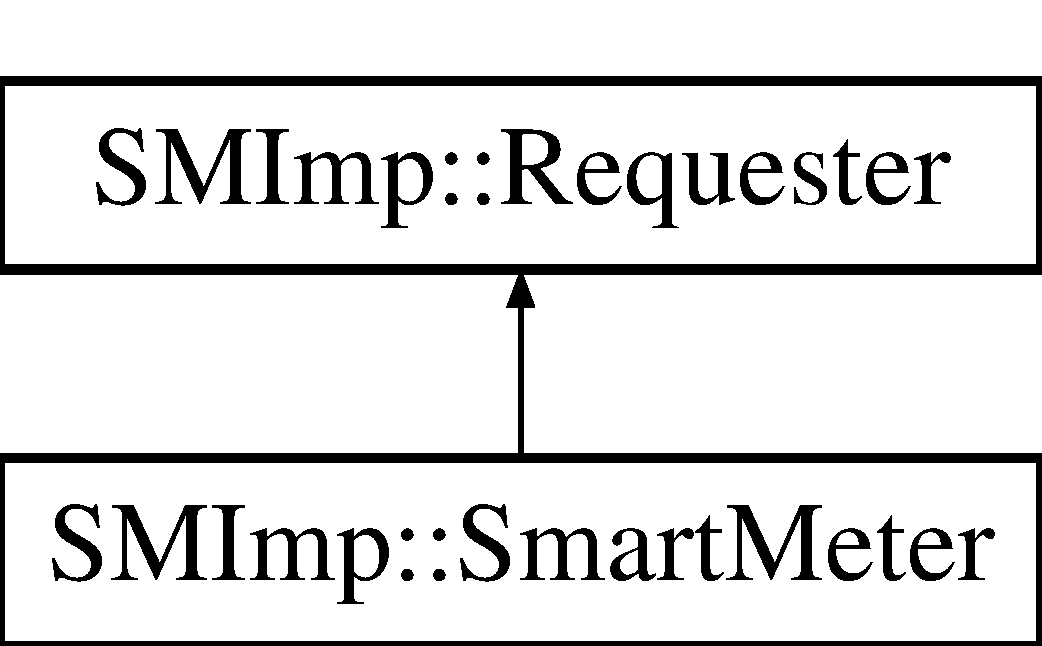
\includegraphics[height=2.000000cm]{classSMImp_1_1SmartMeter}
\end{center}
\end{figure}
\subsection*{Public Member Functions}
\begin{DoxyCompactItemize}
\item 
\hyperlink{classSMImp_1_1SmartMeter_ac677ae1800bcd36e4d599cf3e65463b4}{Smart\+Meter} (Integer, Crypto\+P\+P\+::\+S\+H\+A1 $\ast$)
\item 
\hyperlink{classSMImp_1_1SmartMeter_acadde39bc15942aae2dceb2b4c8c654f}{Smart\+Meter} (Integer, \+::\hyperlink{classSMAdapter}{S\+M\+Adapter} $\ast$)
\item 
\hyperlink{classSMImp_1_1SmartMeter_ae4e756ce74055472a69a0b93f7fd0810}{Smart\+Meter} (Integer)
\item 
virtual \hyperlink{classSMImp_1_1SmartMeter_ace2ebf8736cf495f30a2bc55b1706d73}{$\sim$\+Smart\+Meter} ()
\item 
void \hyperlink{classSMImp_1_1SmartMeter_a577ec9d3df97e40c63e15f3d2f1847af}{set\+H\+M\+A\+C\+Key} (Integer)
\item 
bool \hyperlink{classSMImp_1_1SmartMeter_a38dcb0b09d01582e1322c11638d98fbf}{generate\+Keys} (\hyperlink{structSMImp_1_1Payload}{Payload})
\item 
void \hyperlink{classSMImp_1_1SmartMeter_a4ac0d17fe970851c693d75efc4483094}{set\+Anon\+Id} (Integer)
\item 
Integer \hyperlink{classSMImp_1_1SmartMeter_ad8721f6b2058318e7acf1ce6afa0757d}{get\+Anon\+Id} ()
\item 
\hyperlink{structSMImp_1_1Packet}{Packet} $\ast$ \hyperlink{classSMImp_1_1SmartMeter_ab5248e75260fdd693fe0f5bb3238c249}{send\+Data\+To\+T\+TP} (Integer data)
\item 
\hyperlink{structSMImp_1_1Packet}{Packet} $\ast$ \hyperlink{classSMImp_1_1SmartMeter_a9511926a038ac3ac9c65013f7dd7fb2f}{session\+Key\+Exchange} (char $\ast$m, Integer l, Integer trusted\+Party\+Id, Integer trusted\+Party\+Key, Integer trusted\+Party\+Mu)
\item 
bool \hyperlink{classSMImp_1_1SmartMeter_a489f430377277201d687642d9a58ab80}{recieve\+H\+M\+AC} (Integer c1, Integer c2, Integer ttp\+Id)
\end{DoxyCompactItemize}
\subsection*{Additional Inherited Members}


\subsection{Detailed Description}
Smart Meter protocol implementation. 

Most variables have been named after their respective names given in the original research paper available \href{https://www.researchgate.net/publication/305077004_Secure_and_efficient_protection_of_consumer_privacy_in_Advanced_Metering_Infrastructure_supporting_fine-grained_data_analysis}{\tt here}. See section 5 (Page 7) for the beginning of the protocol implementation. 

Definition at line 15 of file Smart\+Meter.\+h.



\subsection{Constructor \& Destructor Documentation}
\mbox{\Hypertarget{classSMImp_1_1SmartMeter_ac677ae1800bcd36e4d599cf3e65463b4}\label{classSMImp_1_1SmartMeter_ac677ae1800bcd36e4d599cf3e65463b4}} 
\index{S\+M\+Imp\+::\+Smart\+Meter@{S\+M\+Imp\+::\+Smart\+Meter}!Smart\+Meter@{Smart\+Meter}}
\index{Smart\+Meter@{Smart\+Meter}!S\+M\+Imp\+::\+Smart\+Meter@{S\+M\+Imp\+::\+Smart\+Meter}}
\subsubsection{\texorpdfstring{Smart\+Meter()}{SmartMeter()}\hspace{0.1cm}{\footnotesize\ttfamily [1/3]}}
{\footnotesize\ttfamily S\+M\+Imp\+::\+Smart\+Meter\+::\+Smart\+Meter (\begin{DoxyParamCaption}\item[{Integer}]{,  }\item[{Crypto\+P\+P\+::\+S\+H\+A1 $\ast$}]{ }\end{DoxyParamCaption})}

\begin{DoxySeeAlso}{See also}
S\+M\+Imp\+::\+Requester\+::\+Requester(\+Integer,\+S\+H\+A1) 
\end{DoxySeeAlso}
\mbox{\Hypertarget{classSMImp_1_1SmartMeter_acadde39bc15942aae2dceb2b4c8c654f}\label{classSMImp_1_1SmartMeter_acadde39bc15942aae2dceb2b4c8c654f}} 
\index{S\+M\+Imp\+::\+Smart\+Meter@{S\+M\+Imp\+::\+Smart\+Meter}!Smart\+Meter@{Smart\+Meter}}
\index{Smart\+Meter@{Smart\+Meter}!S\+M\+Imp\+::\+Smart\+Meter@{S\+M\+Imp\+::\+Smart\+Meter}}
\subsubsection{\texorpdfstring{Smart\+Meter()}{SmartMeter()}\hspace{0.1cm}{\footnotesize\ttfamily [2/3]}}
{\footnotesize\ttfamily S\+M\+Imp\+::\+Smart\+Meter\+::\+Smart\+Meter (\begin{DoxyParamCaption}\item[{Integer}]{,  }\item[{\+::\hyperlink{classSMAdapter}{S\+M\+Adapter} $\ast$}]{ }\end{DoxyParamCaption})}

For debugging. \mbox{\Hypertarget{classSMImp_1_1SmartMeter_ae4e756ce74055472a69a0b93f7fd0810}\label{classSMImp_1_1SmartMeter_ae4e756ce74055472a69a0b93f7fd0810}} 
\index{S\+M\+Imp\+::\+Smart\+Meter@{S\+M\+Imp\+::\+Smart\+Meter}!Smart\+Meter@{Smart\+Meter}}
\index{Smart\+Meter@{Smart\+Meter}!S\+M\+Imp\+::\+Smart\+Meter@{S\+M\+Imp\+::\+Smart\+Meter}}
\subsubsection{\texorpdfstring{Smart\+Meter()}{SmartMeter()}\hspace{0.1cm}{\footnotesize\ttfamily [3/3]}}
{\footnotesize\ttfamily S\+M\+Imp\+::\+Smart\+Meter\+::\+Smart\+Meter (\begin{DoxyParamCaption}\item[{Integer}]{i }\end{DoxyParamCaption})}



Definition at line 34 of file Smart\+Meter.\+cc.



References S\+M\+Imp\+::\+Requester\+::\+Requester(), and Smart\+Meter().

\mbox{\Hypertarget{classSMImp_1_1SmartMeter_ace2ebf8736cf495f30a2bc55b1706d73}\label{classSMImp_1_1SmartMeter_ace2ebf8736cf495f30a2bc55b1706d73}} 
\index{S\+M\+Imp\+::\+Smart\+Meter@{S\+M\+Imp\+::\+Smart\+Meter}!````~Smart\+Meter@{$\sim$\+Smart\+Meter}}
\index{````~Smart\+Meter@{$\sim$\+Smart\+Meter}!S\+M\+Imp\+::\+Smart\+Meter@{S\+M\+Imp\+::\+Smart\+Meter}}
\subsubsection{\texorpdfstring{$\sim$\+Smart\+Meter()}{~SmartMeter()}}
{\footnotesize\ttfamily S\+M\+Imp\+::\+Smart\+Meter\+::$\sim$\+Smart\+Meter (\begin{DoxyParamCaption}{ }\end{DoxyParamCaption})\hspace{0.3cm}{\ttfamily [virtual]}}



Definition at line 49 of file Smart\+Meter.\+cc.



\subsection{Member Function Documentation}
\mbox{\Hypertarget{classSMImp_1_1SmartMeter_a38dcb0b09d01582e1322c11638d98fbf}\label{classSMImp_1_1SmartMeter_a38dcb0b09d01582e1322c11638d98fbf}} 
\index{S\+M\+Imp\+::\+Smart\+Meter@{S\+M\+Imp\+::\+Smart\+Meter}!generate\+Keys@{generate\+Keys}}
\index{generate\+Keys@{generate\+Keys}!S\+M\+Imp\+::\+Smart\+Meter@{S\+M\+Imp\+::\+Smart\+Meter}}
\subsubsection{\texorpdfstring{generate\+Keys()}{generateKeys()}}
{\footnotesize\ttfamily bool S\+M\+Imp\+::\+Smart\+Meter\+::generate\+Keys (\begin{DoxyParamCaption}\item[{\hyperlink{structSMImp_1_1Payload}{Payload}}]{pl }\end{DoxyParamCaption})}

Generates keys from payload given by Utility Company. 

Definition at line 11 of file Smart\+Meter.\+cc.



References S\+M\+Imp\+::\+Master\+Key\+::g, S\+M\+Imp\+::\+Requester\+::get\+Partials(), S\+M\+Imp\+::\+Requester\+::keys, S\+M\+Imp\+::\+Master\+Key\+::p, S\+M\+Imp\+::\+Requester\+::params, S\+M\+Imp\+::\+Key\+::piece, S\+M\+Imp\+::\+Key\+Pair\+::priv, S\+M\+Imp\+::\+Key\+Pair\+::pub, S\+M\+Imp\+::\+Master\+Key\+::q, and S\+M\+Imp\+::\+Requester\+::rng.

\mbox{\Hypertarget{classSMImp_1_1SmartMeter_ad8721f6b2058318e7acf1ce6afa0757d}\label{classSMImp_1_1SmartMeter_ad8721f6b2058318e7acf1ce6afa0757d}} 
\index{S\+M\+Imp\+::\+Smart\+Meter@{S\+M\+Imp\+::\+Smart\+Meter}!get\+Anon\+Id@{get\+Anon\+Id}}
\index{get\+Anon\+Id@{get\+Anon\+Id}!S\+M\+Imp\+::\+Smart\+Meter@{S\+M\+Imp\+::\+Smart\+Meter}}
\subsubsection{\texorpdfstring{get\+Anon\+Id()}{getAnonId()}}
{\footnotesize\ttfamily Integer S\+M\+Imp\+::\+Smart\+Meter\+::get\+Anon\+Id (\begin{DoxyParamCaption}{ }\end{DoxyParamCaption})}

\begin{DoxySeeAlso}{See also}
S\+M\+Imp\+::\+Requester\+::get\+Anon\+Id() 
\end{DoxySeeAlso}


Definition at line 53 of file Smart\+Meter.\+cc.

\mbox{\Hypertarget{classSMImp_1_1SmartMeter_a489f430377277201d687642d9a58ab80}\label{classSMImp_1_1SmartMeter_a489f430377277201d687642d9a58ab80}} 
\index{S\+M\+Imp\+::\+Smart\+Meter@{S\+M\+Imp\+::\+Smart\+Meter}!recieve\+H\+M\+AC@{recieve\+H\+M\+AC}}
\index{recieve\+H\+M\+AC@{recieve\+H\+M\+AC}!S\+M\+Imp\+::\+Smart\+Meter@{S\+M\+Imp\+::\+Smart\+Meter}}
\subsubsection{\texorpdfstring{recieve\+H\+M\+A\+C()}{recieveHMAC()}}
{\footnotesize\ttfamily bool S\+M\+Imp\+::\+Smart\+Meter\+::recieve\+H\+M\+AC (\begin{DoxyParamCaption}\item[{Integer}]{c1,  }\item[{Integer}]{c2,  }\item[{Integer}]{ttp\+Id }\end{DoxyParamCaption})}

Used at the end of the session key exchange phase. H\+M\+AC verifies, then decrypts the final shared session key. 
\begin{DoxyParams}{Parameters}
{\em c1} & Part 1 of the encrypted session key. \\
\hline
{\em c2} & Part 2 of the encrypted session key. \\
\hline
{\em ttp\+Id} & ID of the Trusted Third Party. \\
\hline
\end{DoxyParams}


Definition at line 221 of file Smart\+Meter.\+cc.



References S\+M\+Adapter\+::add\+Sim\+Time(), S\+M\+Imp\+::\+Master\+Key\+::g, S\+M\+Imp\+::\+Requester\+::keys, S\+M\+Adapter\+::log(), S\+M\+Imp\+::\+Master\+Key\+::p, S\+M\+Imp\+::\+Requester\+::params, S\+M\+Imp\+::\+Key\+::partial, S\+M\+Imp\+::\+Key\+::piece, and S\+M\+Imp\+::\+Key\+Pair\+::priv.

\mbox{\Hypertarget{classSMImp_1_1SmartMeter_ab5248e75260fdd693fe0f5bb3238c249}\label{classSMImp_1_1SmartMeter_ab5248e75260fdd693fe0f5bb3238c249}} 
\index{S\+M\+Imp\+::\+Smart\+Meter@{S\+M\+Imp\+::\+Smart\+Meter}!send\+Data\+To\+T\+TP@{send\+Data\+To\+T\+TP}}
\index{send\+Data\+To\+T\+TP@{send\+Data\+To\+T\+TP}!S\+M\+Imp\+::\+Smart\+Meter@{S\+M\+Imp\+::\+Smart\+Meter}}
\subsubsection{\texorpdfstring{send\+Data\+To\+T\+T\+P()}{sendDataToTTP()}}
{\footnotesize\ttfamily \hyperlink{structSMImp_1_1Packet}{Packet} $\ast$ S\+M\+Imp\+::\+Smart\+Meter\+::send\+Data\+To\+T\+TP (\begin{DoxyParamCaption}\item[{Integer}]{data }\end{DoxyParamCaption})}

Encrypts data to be sent to the Trusted Thrid Party. 
\begin{DoxyParams}{Parameters}
{\em data} & Data to be encrypted and sent to Trusted Thrid Party. \\
\hline
\end{DoxyParams}
\begin{DoxyReturn}{Returns}
\hyperlink{structSMImp_1_1Packet}{Packet} of encrypted data. 
\end{DoxyReturn}


Definition at line 69 of file Smart\+Meter.\+cc.



References S\+M\+Adapter\+::add\+Sim\+Time(), S\+M\+Imp\+::\+H\+M\+A\+C\+Payload\+::c1, S\+M\+Imp\+::\+H\+M\+A\+C\+Payload\+::c2, D\+E\+B\+UG, S\+M\+Imp\+::\+Master\+Key\+::g, S\+M\+Imp\+::\+H\+M\+A\+C\+Payload\+::hmac, S\+M\+Imp\+::\+Requester\+::id, S\+M\+Imp\+::\+H\+M\+A\+C\+Payload\+::id, S\+M\+Adapter\+::log(), S\+M\+Imp\+::\+H\+M\+A\+C\+Payload\+::message\+Length, S\+M\+Imp\+::\+Master\+Key\+::p, S\+M\+Imp\+::\+Requester\+::params, S\+M\+Imp\+::\+Packet\+::pl, S\+M\+Imp\+::\+Requester\+::R, S\+M\+Imp\+::\+H\+M\+A\+C\+Payload\+::r, S\+M\+Imp\+::\+Requester\+::shaone, S\+M\+Imp\+::\+H\+M\+A\+C\+Payload\+::time\+Stamp, and S\+M\+Imp\+::\+Master\+Key\+::x.

\mbox{\Hypertarget{classSMImp_1_1SmartMeter_a9511926a038ac3ac9c65013f7dd7fb2f}\label{classSMImp_1_1SmartMeter_a9511926a038ac3ac9c65013f7dd7fb2f}} 
\index{S\+M\+Imp\+::\+Smart\+Meter@{S\+M\+Imp\+::\+Smart\+Meter}!session\+Key\+Exchange@{session\+Key\+Exchange}}
\index{session\+Key\+Exchange@{session\+Key\+Exchange}!S\+M\+Imp\+::\+Smart\+Meter@{S\+M\+Imp\+::\+Smart\+Meter}}
\subsubsection{\texorpdfstring{session\+Key\+Exchange()}{sessionKeyExchange()}}
{\footnotesize\ttfamily \hyperlink{structSMImp_1_1Packet}{Packet} $\ast$ S\+M\+Imp\+::\+Smart\+Meter\+::session\+Key\+Exchange (\begin{DoxyParamCaption}\item[{char $\ast$}]{m,  }\item[{Integer}]{l,  }\item[{Integer}]{trusted\+Party\+Id,  }\item[{Integer}]{trusted\+Party\+Key,  }\item[{Integer}]{trusted\+Party\+Mu }\end{DoxyParamCaption})}

Performs all the processes to both generate and split up the session key, returning an array of packets to encasulate in the \hyperlink{classAdapter}{Adapter}. 
\begin{DoxyParams}{Parameters}
{\em m} & Message, or the session key to be generated, see S\+M\+Adaoter\+::start\+Session\+Key\+Exchange(omnetpp\+::c\+Message$\ast$ msg). \\
\hline
{\em l} & Length of the session key, does not need to be a multiple of 4 since char(\textquotesingle{}0\textquotesingle{})s (or int(48)) are padded to reach the desired length. \\
\hline
{\em trusted\+Party\+Id} & ID of the Trusted Third Party to share a session key with. \\
\hline
{\em trusted\+Party\+Key} & Missnamed variable, this is just the first piece of the public key -\/ specificially the component generated by the Utility Company. \\
\hline
{\em trusted\+Party\+Mu} & second peice of the public key, generated by the Trusted Third Party. \\
\hline
\end{DoxyParams}
\begin{DoxyReturn}{Returns}
Returns array of messages to be encapsulated and sent to Trusted Third Party. Array is of length (l+(4-\/(l\%4)))/4, or ceiling(l/4) where l is the length of the session key. 
\end{DoxyReturn}


Definition at line 130 of file Smart\+Meter.\+cc.



References S\+M\+Adapter\+::add\+Sim\+Time(), S\+M\+Imp\+::\+H\+M\+A\+C\+Payload\+::c1, S\+M\+Imp\+::\+H\+M\+A\+C\+Payload\+::c2, S\+M\+Imp\+::\+Packet\+::dest, S\+M\+Imp\+::\+Master\+Key\+::g, S\+M\+Imp\+::\+H\+M\+A\+C\+Payload\+::hmac, S\+M\+Imp\+::\+Requester\+::id, S\+M\+Imp\+::\+H\+M\+A\+C\+Payload\+::id, S\+M\+Adapter\+::log(), S\+M\+Imp\+::\+H\+M\+A\+C\+Payload\+::message\+Length, S\+M\+Imp\+::\+Master\+Key\+::p, S\+M\+Imp\+::\+Requester\+::params, S\+M\+Imp\+::\+Packet\+::pl, S\+M\+Imp\+::\+Requester\+::R, S\+M\+Imp\+::\+H\+M\+A\+C\+Payload\+::r, S\+M\+Imp\+::\+Requester\+::rng, S\+M\+Imp\+::\+Requester\+::shaone, S\+M\+Imp\+::\+H\+M\+A\+C\+Payload\+::time\+Stamp, and S\+M\+Imp\+::\+Master\+Key\+::x.

\mbox{\Hypertarget{classSMImp_1_1SmartMeter_a4ac0d17fe970851c693d75efc4483094}\label{classSMImp_1_1SmartMeter_a4ac0d17fe970851c693d75efc4483094}} 
\index{S\+M\+Imp\+::\+Smart\+Meter@{S\+M\+Imp\+::\+Smart\+Meter}!set\+Anon\+Id@{set\+Anon\+Id}}
\index{set\+Anon\+Id@{set\+Anon\+Id}!S\+M\+Imp\+::\+Smart\+Meter@{S\+M\+Imp\+::\+Smart\+Meter}}
\subsubsection{\texorpdfstring{set\+Anon\+Id()}{setAnonId()}}
{\footnotesize\ttfamily void S\+M\+Imp\+::\+Smart\+Meter\+::set\+Anon\+Id (\begin{DoxyParamCaption}\item[{Integer}]{a }\end{DoxyParamCaption})}

Sets the anonymous ID 

Definition at line 58 of file Smart\+Meter.\+cc.

\mbox{\Hypertarget{classSMImp_1_1SmartMeter_a577ec9d3df97e40c63e15f3d2f1847af}\label{classSMImp_1_1SmartMeter_a577ec9d3df97e40c63e15f3d2f1847af}} 
\index{S\+M\+Imp\+::\+Smart\+Meter@{S\+M\+Imp\+::\+Smart\+Meter}!set\+H\+M\+A\+C\+Key@{set\+H\+M\+A\+C\+Key}}
\index{set\+H\+M\+A\+C\+Key@{set\+H\+M\+A\+C\+Key}!S\+M\+Imp\+::\+Smart\+Meter@{S\+M\+Imp\+::\+Smart\+Meter}}
\subsubsection{\texorpdfstring{set\+H\+M\+A\+C\+Key()}{setHMACKey()}}
{\footnotesize\ttfamily void S\+M\+Imp\+::\+Smart\+Meter\+::set\+H\+M\+A\+C\+Key (\begin{DoxyParamCaption}\item[{Integer}]{i }\end{DoxyParamCaption})}

Sets H\+M\+AC to be used for verification. 

Definition at line 63 of file Smart\+Meter.\+cc.



The documentation for this class was generated from the following files\+:\begin{DoxyCompactItemize}
\item 
src/crypto/\hyperlink{crypto_2SmartMeter_8h}{Smart\+Meter.\+h}\item 
src/crypto/\hyperlink{crypto_2SmartMeter_8cc}{Smart\+Meter.\+cc}\end{DoxyCompactItemize}

\hypertarget{classsmart3p_1_1SMPacket}{}\section{smart3p\+:\+:S\+M\+Packet Class Reference}
\label{classsmart3p_1_1SMPacket}\index{smart3p\+::\+S\+M\+Packet@{smart3p\+::\+S\+M\+Packet}}


{\ttfamily \#include $<$S\+M\+Packet\+\_\+m.\+h$>$}

Inheritance diagram for smart3p\+:\+:S\+M\+Packet\+:\begin{figure}[H]
\begin{center}
\leavevmode
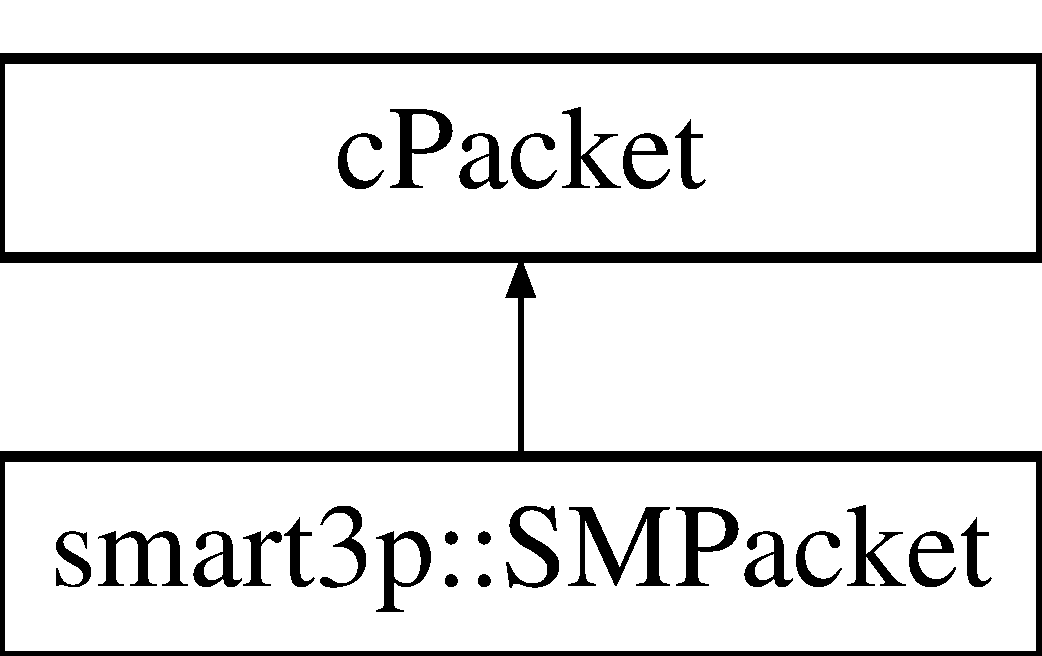
\includegraphics[height=2.000000cm]{classsmart3p_1_1SMPacket}
\end{center}
\end{figure}
\subsection*{Public Member Functions}
\begin{DoxyCompactItemize}
\item 
\hyperlink{classsmart3p_1_1SMPacket_a096748da42a5fce6a6947268987c1a62}{S\+M\+Packet} (const char $\ast$name=nullptr, int kind=0)
\item 
\hyperlink{classsmart3p_1_1SMPacket_ab998efe53cce923572c1ca4d147fef57}{S\+M\+Packet} (const \hyperlink{classsmart3p_1_1SMPacket}{S\+M\+Packet} \&other)
\item 
virtual \hyperlink{classsmart3p_1_1SMPacket_ab5e176e11c65abb458f17f75ccad4344}{$\sim$\+S\+M\+Packet} ()
\item 
\hyperlink{classsmart3p_1_1SMPacket}{S\+M\+Packet} \& \hyperlink{classsmart3p_1_1SMPacket_a9f61efd109fbd0c599a9fd07309392f4}{operator=} (const \hyperlink{classsmart3p_1_1SMPacket}{S\+M\+Packet} \&other)
\item 
virtual \hyperlink{classsmart3p_1_1SMPacket}{S\+M\+Packet} $\ast$ \hyperlink{classsmart3p_1_1SMPacket_a94d4fe6ad55564e56212f96d9b65e346}{dup} () const
\item 
virtual void \hyperlink{classsmart3p_1_1SMPacket_a68dbbbae28db832e790118a6f55c662b}{parsim\+Pack} (omnetpp\+::c\+Comm\+Buffer $\ast$b) const
\item 
virtual void \hyperlink{classsmart3p_1_1SMPacket_a758324526341dcbd38b8bdb21327b1e2}{parsim\+Unpack} (omnetpp\+::c\+Comm\+Buffer $\ast$b)
\item 
virtual int \hyperlink{classsmart3p_1_1SMPacket_a4c1e98a2f81acc1addcae93531e72af1}{get\+Id} () const
\item 
virtual void \hyperlink{classsmart3p_1_1SMPacket_a9ba1e3a6882f264a5c26598db65f2c16}{set\+Id} (int \hyperlink{classsmart3p_1_1SMPacket_af0612d8448370b8919ff415b860725ed}{id})
\item 
virtual double \hyperlink{classsmart3p_1_1SMPacket_a4278cf44eab393e432f284f8e846c602}{get\+Value} () const
\item 
virtual void \hyperlink{classsmart3p_1_1SMPacket_a19a0aa3959661f34bc16de6411e46daa}{set\+Value} (double \hyperlink{classsmart3p_1_1SMPacket_aa5596bff5a9720c59788a6766357c8d9}{value})
\item 
virtual int \hyperlink{classsmart3p_1_1SMPacket_a157ffd9338082090b11995f78e863e0d}{get\+Sm\+Gate\+ID} () const
\item 
virtual void \hyperlink{classsmart3p_1_1SMPacket_ad29377a4b1e784290e99c4bf538fbeef}{set\+Sm\+Gate\+ID} (int \hyperlink{classsmart3p_1_1SMPacket_a12d57198d78f1b58b027aba4a99cdc3b}{sm\+Gate\+ID})
\item 
virtual int \hyperlink{classsmart3p_1_1SMPacket_a64547473581a84a343c77f9f4b4257c5}{get\+Coll\+Gate\+ID} () const
\item 
virtual void \hyperlink{classsmart3p_1_1SMPacket_ae1249b367e1c92820a7f79f50efcc348}{set\+Coll\+Gate\+ID} (int \hyperlink{classsmart3p_1_1SMPacket_ae81077057b1f59dab392f09966529047}{coll\+Gate\+ID})
\item 
virtual const char $\ast$ \hyperlink{classsmart3p_1_1SMPacket_a58f21f2e289fbc7910ef3e5ef7d05c3b}{get\+Extra\+Info} () const
\item 
virtual void \hyperlink{classsmart3p_1_1SMPacket_a3ab2306b41ed54f86e97f5163a7f3ae9}{set\+Extra\+Info} (const char $\ast$\hyperlink{classsmart3p_1_1SMPacket_acff575715f936a984686d4bd618570e9}{extra\+Info})
\item 
virtual const char $\ast$ \hyperlink{classsmart3p_1_1SMPacket_a54975c6966ddb5994442161e0b68aa30}{get\+Extra\+Info\+Size} () const
\item 
virtual void \hyperlink{classsmart3p_1_1SMPacket_a4012df901869826bdd19394312489ce8}{set\+Extra\+Info\+Size} (const char $\ast$\hyperlink{classsmart3p_1_1SMPacket_a546cc7b651dd40a4ee98990fabd10f5c}{extra\+Info\+Size})
\end{DoxyCompactItemize}
\subsection*{Protected Member Functions}
\begin{DoxyCompactItemize}
\item 
bool \hyperlink{classsmart3p_1_1SMPacket_a999e29404cc37d5b92ff52ab862d246b}{operator==} (const \hyperlink{classsmart3p_1_1SMPacket}{S\+M\+Packet} \&)
\end{DoxyCompactItemize}
\subsection*{Protected Attributes}
\begin{DoxyCompactItemize}
\item 
int \hyperlink{classsmart3p_1_1SMPacket_af0612d8448370b8919ff415b860725ed}{id}
\item 
double \hyperlink{classsmart3p_1_1SMPacket_aa5596bff5a9720c59788a6766357c8d9}{value}
\item 
int \hyperlink{classsmart3p_1_1SMPacket_a12d57198d78f1b58b027aba4a99cdc3b}{sm\+Gate\+ID}
\item 
int \hyperlink{classsmart3p_1_1SMPacket_ae81077057b1f59dab392f09966529047}{coll\+Gate\+ID}
\item 
\+::omnetpp\+::opp\+\_\+string \hyperlink{classsmart3p_1_1SMPacket_acff575715f936a984686d4bd618570e9}{extra\+Info}
\item 
\+::omnetpp\+::opp\+\_\+string \hyperlink{classsmart3p_1_1SMPacket_a546cc7b651dd40a4ee98990fabd10f5c}{extra\+Info\+Size}
\end{DoxyCompactItemize}


\subsection{Detailed Description}
Class generated from {\ttfamily S\+M\+Packet.\+msg\+:6} by nedtool. 
\begin{DoxyPre}
   //
   // Smart Meter Packet
   //
   packet \hyperlink{classsmart3p_1_1SMPacket}{SMPacket}
   \{
       int id;
       double value;
       int smGateID;
       int collGateID;
       string extraInfo;
       string extraInfoSize;
   \}
   \end{DoxyPre}
 o 

Definition at line 36 of file S\+M\+Packet\+\_\+m.\+h.



\subsection{Constructor \& Destructor Documentation}
\mbox{\Hypertarget{classsmart3p_1_1SMPacket_a096748da42a5fce6a6947268987c1a62}\label{classsmart3p_1_1SMPacket_a096748da42a5fce6a6947268987c1a62}} 
\index{smart3p\+::\+S\+M\+Packet@{smart3p\+::\+S\+M\+Packet}!S\+M\+Packet@{S\+M\+Packet}}
\index{S\+M\+Packet@{S\+M\+Packet}!smart3p\+::\+S\+M\+Packet@{smart3p\+::\+S\+M\+Packet}}
\subsubsection{\texorpdfstring{S\+M\+Packet()}{SMPacket()}\hspace{0.1cm}{\footnotesize\ttfamily [1/2]}}
{\footnotesize\ttfamily smart3p\+::\+S\+M\+Packet\+::\+S\+M\+Packet (\begin{DoxyParamCaption}\item[{const char $\ast$}]{name = {\ttfamily nullptr},  }\item[{int}]{kind = {\ttfamily 0} }\end{DoxyParamCaption})}



Definition at line 167 of file S\+M\+Packet\+\_\+m.\+cc.



References coll\+Gate\+ID, sm\+Gate\+ID, and value.

\mbox{\Hypertarget{classsmart3p_1_1SMPacket_ab998efe53cce923572c1ca4d147fef57}\label{classsmart3p_1_1SMPacket_ab998efe53cce923572c1ca4d147fef57}} 
\index{smart3p\+::\+S\+M\+Packet@{smart3p\+::\+S\+M\+Packet}!S\+M\+Packet@{S\+M\+Packet}}
\index{S\+M\+Packet@{S\+M\+Packet}!smart3p\+::\+S\+M\+Packet@{smart3p\+::\+S\+M\+Packet}}
\subsubsection{\texorpdfstring{S\+M\+Packet()}{SMPacket()}\hspace{0.1cm}{\footnotesize\ttfamily [2/2]}}
{\footnotesize\ttfamily smart3p\+::\+S\+M\+Packet\+::\+S\+M\+Packet (\begin{DoxyParamCaption}\item[{const \hyperlink{classsmart3p_1_1SMPacket}{S\+M\+Packet} \&}]{other }\end{DoxyParamCaption})}



Definition at line 175 of file S\+M\+Packet\+\_\+m.\+cc.

\mbox{\Hypertarget{classsmart3p_1_1SMPacket_ab5e176e11c65abb458f17f75ccad4344}\label{classsmart3p_1_1SMPacket_ab5e176e11c65abb458f17f75ccad4344}} 
\index{smart3p\+::\+S\+M\+Packet@{smart3p\+::\+S\+M\+Packet}!````~S\+M\+Packet@{$\sim$\+S\+M\+Packet}}
\index{````~S\+M\+Packet@{$\sim$\+S\+M\+Packet}!smart3p\+::\+S\+M\+Packet@{smart3p\+::\+S\+M\+Packet}}
\subsubsection{\texorpdfstring{$\sim$\+S\+M\+Packet()}{~SMPacket()}}
{\footnotesize\ttfamily smart3p\+::\+S\+M\+Packet\+::$\sim$\+S\+M\+Packet (\begin{DoxyParamCaption}{ }\end{DoxyParamCaption})\hspace{0.3cm}{\ttfamily [virtual]}}



Definition at line 180 of file S\+M\+Packet\+\_\+m.\+cc.



\subsection{Member Function Documentation}
\mbox{\Hypertarget{classsmart3p_1_1SMPacket_a94d4fe6ad55564e56212f96d9b65e346}\label{classsmart3p_1_1SMPacket_a94d4fe6ad55564e56212f96d9b65e346}} 
\index{smart3p\+::\+S\+M\+Packet@{smart3p\+::\+S\+M\+Packet}!dup@{dup}}
\index{dup@{dup}!smart3p\+::\+S\+M\+Packet@{smart3p\+::\+S\+M\+Packet}}
\subsubsection{\texorpdfstring{dup()}{dup()}}
{\footnotesize\ttfamily virtual \hyperlink{classsmart3p_1_1SMPacket}{S\+M\+Packet}$\ast$ smart3p\+::\+S\+M\+Packet\+::dup (\begin{DoxyParamCaption}{ }\end{DoxyParamCaption}) const\hspace{0.3cm}{\ttfamily [inline]}, {\ttfamily [virtual]}}



Definition at line 58 of file S\+M\+Packet\+\_\+m.\+h.



References get\+Coll\+Gate\+I\+D(), get\+Extra\+Info(), get\+Extra\+Info\+Size(), get\+Id(), get\+Sm\+Gate\+I\+D(), get\+Value(), parsim\+Pack(), parsim\+Unpack(), set\+Coll\+Gate\+I\+D(), set\+Extra\+Info(), set\+Extra\+Info\+Size(), set\+Id(), set\+Sm\+Gate\+I\+D(), set\+Value(), and S\+M\+Packet().

\mbox{\Hypertarget{classsmart3p_1_1SMPacket_a64547473581a84a343c77f9f4b4257c5}\label{classsmart3p_1_1SMPacket_a64547473581a84a343c77f9f4b4257c5}} 
\index{smart3p\+::\+S\+M\+Packet@{smart3p\+::\+S\+M\+Packet}!get\+Coll\+Gate\+ID@{get\+Coll\+Gate\+ID}}
\index{get\+Coll\+Gate\+ID@{get\+Coll\+Gate\+ID}!smart3p\+::\+S\+M\+Packet@{smart3p\+::\+S\+M\+Packet}}
\subsubsection{\texorpdfstring{get\+Coll\+Gate\+I\+D()}{getCollGateID()}}
{\footnotesize\ttfamily int smart3p\+::\+S\+M\+Packet\+::get\+Coll\+Gate\+ID (\begin{DoxyParamCaption}{ }\end{DoxyParamCaption}) const\hspace{0.3cm}{\ttfamily [virtual]}}



Definition at line 254 of file S\+M\+Packet\+\_\+m.\+cc.



References coll\+Gate\+ID.

\mbox{\Hypertarget{classsmart3p_1_1SMPacket_a58f21f2e289fbc7910ef3e5ef7d05c3b}\label{classsmart3p_1_1SMPacket_a58f21f2e289fbc7910ef3e5ef7d05c3b}} 
\index{smart3p\+::\+S\+M\+Packet@{smart3p\+::\+S\+M\+Packet}!get\+Extra\+Info@{get\+Extra\+Info}}
\index{get\+Extra\+Info@{get\+Extra\+Info}!smart3p\+::\+S\+M\+Packet@{smart3p\+::\+S\+M\+Packet}}
\subsubsection{\texorpdfstring{get\+Extra\+Info()}{getExtraInfo()}}
{\footnotesize\ttfamily const char $\ast$ smart3p\+::\+S\+M\+Packet\+::get\+Extra\+Info (\begin{DoxyParamCaption}{ }\end{DoxyParamCaption}) const\hspace{0.3cm}{\ttfamily [virtual]}}



Definition at line 264 of file S\+M\+Packet\+\_\+m.\+cc.



References extra\+Info.

\mbox{\Hypertarget{classsmart3p_1_1SMPacket_a54975c6966ddb5994442161e0b68aa30}\label{classsmart3p_1_1SMPacket_a54975c6966ddb5994442161e0b68aa30}} 
\index{smart3p\+::\+S\+M\+Packet@{smart3p\+::\+S\+M\+Packet}!get\+Extra\+Info\+Size@{get\+Extra\+Info\+Size}}
\index{get\+Extra\+Info\+Size@{get\+Extra\+Info\+Size}!smart3p\+::\+S\+M\+Packet@{smart3p\+::\+S\+M\+Packet}}
\subsubsection{\texorpdfstring{get\+Extra\+Info\+Size()}{getExtraInfoSize()}}
{\footnotesize\ttfamily const char $\ast$ smart3p\+::\+S\+M\+Packet\+::get\+Extra\+Info\+Size (\begin{DoxyParamCaption}{ }\end{DoxyParamCaption}) const\hspace{0.3cm}{\ttfamily [virtual]}}



Definition at line 274 of file S\+M\+Packet\+\_\+m.\+cc.



References extra\+Info\+Size.

\mbox{\Hypertarget{classsmart3p_1_1SMPacket_a4c1e98a2f81acc1addcae93531e72af1}\label{classsmart3p_1_1SMPacket_a4c1e98a2f81acc1addcae93531e72af1}} 
\index{smart3p\+::\+S\+M\+Packet@{smart3p\+::\+S\+M\+Packet}!get\+Id@{get\+Id}}
\index{get\+Id@{get\+Id}!smart3p\+::\+S\+M\+Packet@{smart3p\+::\+S\+M\+Packet}}
\subsubsection{\texorpdfstring{get\+Id()}{getId()}}
{\footnotesize\ttfamily int smart3p\+::\+S\+M\+Packet\+::get\+Id (\begin{DoxyParamCaption}{ }\end{DoxyParamCaption}) const\hspace{0.3cm}{\ttfamily [virtual]}}



Definition at line 224 of file S\+M\+Packet\+\_\+m.\+cc.



References id.

\mbox{\Hypertarget{classsmart3p_1_1SMPacket_a157ffd9338082090b11995f78e863e0d}\label{classsmart3p_1_1SMPacket_a157ffd9338082090b11995f78e863e0d}} 
\index{smart3p\+::\+S\+M\+Packet@{smart3p\+::\+S\+M\+Packet}!get\+Sm\+Gate\+ID@{get\+Sm\+Gate\+ID}}
\index{get\+Sm\+Gate\+ID@{get\+Sm\+Gate\+ID}!smart3p\+::\+S\+M\+Packet@{smart3p\+::\+S\+M\+Packet}}
\subsubsection{\texorpdfstring{get\+Sm\+Gate\+I\+D()}{getSmGateID()}}
{\footnotesize\ttfamily int smart3p\+::\+S\+M\+Packet\+::get\+Sm\+Gate\+ID (\begin{DoxyParamCaption}{ }\end{DoxyParamCaption}) const\hspace{0.3cm}{\ttfamily [virtual]}}



Definition at line 244 of file S\+M\+Packet\+\_\+m.\+cc.



References sm\+Gate\+ID.

\mbox{\Hypertarget{classsmart3p_1_1SMPacket_a4278cf44eab393e432f284f8e846c602}\label{classsmart3p_1_1SMPacket_a4278cf44eab393e432f284f8e846c602}} 
\index{smart3p\+::\+S\+M\+Packet@{smart3p\+::\+S\+M\+Packet}!get\+Value@{get\+Value}}
\index{get\+Value@{get\+Value}!smart3p\+::\+S\+M\+Packet@{smart3p\+::\+S\+M\+Packet}}
\subsubsection{\texorpdfstring{get\+Value()}{getValue()}}
{\footnotesize\ttfamily double smart3p\+::\+S\+M\+Packet\+::get\+Value (\begin{DoxyParamCaption}{ }\end{DoxyParamCaption}) const\hspace{0.3cm}{\ttfamily [virtual]}}



Definition at line 234 of file S\+M\+Packet\+\_\+m.\+cc.



References value.

\mbox{\Hypertarget{classsmart3p_1_1SMPacket_a9f61efd109fbd0c599a9fd07309392f4}\label{classsmart3p_1_1SMPacket_a9f61efd109fbd0c599a9fd07309392f4}} 
\index{smart3p\+::\+S\+M\+Packet@{smart3p\+::\+S\+M\+Packet}!operator=@{operator=}}
\index{operator=@{operator=}!smart3p\+::\+S\+M\+Packet@{smart3p\+::\+S\+M\+Packet}}
\subsubsection{\texorpdfstring{operator=()}{operator=()}}
{\footnotesize\ttfamily \hyperlink{classsmart3p_1_1SMPacket}{S\+M\+Packet} \& smart3p\+::\+S\+M\+Packet\+::operator= (\begin{DoxyParamCaption}\item[{const \hyperlink{classsmart3p_1_1SMPacket}{S\+M\+Packet} \&}]{other }\end{DoxyParamCaption})}



Definition at line 184 of file S\+M\+Packet\+\_\+m.\+cc.



References coll\+Gate\+ID, extra\+Info, extra\+Info\+Size, id, sm\+Gate\+ID, and value.

\mbox{\Hypertarget{classsmart3p_1_1SMPacket_a999e29404cc37d5b92ff52ab862d246b}\label{classsmart3p_1_1SMPacket_a999e29404cc37d5b92ff52ab862d246b}} 
\index{smart3p\+::\+S\+M\+Packet@{smart3p\+::\+S\+M\+Packet}!operator==@{operator==}}
\index{operator==@{operator==}!smart3p\+::\+S\+M\+Packet@{smart3p\+::\+S\+M\+Packet}}
\subsubsection{\texorpdfstring{operator==()}{operator==()}}
{\footnotesize\ttfamily bool smart3p\+::\+S\+M\+Packet\+::operator== (\begin{DoxyParamCaption}\item[{const \hyperlink{classsmart3p_1_1SMPacket}{S\+M\+Packet} \&}]{ }\end{DoxyParamCaption})\hspace{0.3cm}{\ttfamily [protected]}}

\mbox{\Hypertarget{classsmart3p_1_1SMPacket_a68dbbbae28db832e790118a6f55c662b}\label{classsmart3p_1_1SMPacket_a68dbbbae28db832e790118a6f55c662b}} 
\index{smart3p\+::\+S\+M\+Packet@{smart3p\+::\+S\+M\+Packet}!parsim\+Pack@{parsim\+Pack}}
\index{parsim\+Pack@{parsim\+Pack}!smart3p\+::\+S\+M\+Packet@{smart3p\+::\+S\+M\+Packet}}
\subsubsection{\texorpdfstring{parsim\+Pack()}{parsimPack()}}
{\footnotesize\ttfamily void smart3p\+::\+S\+M\+Packet\+::parsim\+Pack (\begin{DoxyParamCaption}\item[{omnetpp\+::c\+Comm\+Buffer $\ast$}]{b }\end{DoxyParamCaption}) const\hspace{0.3cm}{\ttfamily [virtual]}}



Definition at line 202 of file S\+M\+Packet\+\_\+m.\+cc.



References coll\+Gate\+ID, smart3p\+::do\+Parsim\+Packing(), extra\+Info, extra\+Info\+Size, sm\+Gate\+ID, and value.

\mbox{\Hypertarget{classsmart3p_1_1SMPacket_a758324526341dcbd38b8bdb21327b1e2}\label{classsmart3p_1_1SMPacket_a758324526341dcbd38b8bdb21327b1e2}} 
\index{smart3p\+::\+S\+M\+Packet@{smart3p\+::\+S\+M\+Packet}!parsim\+Unpack@{parsim\+Unpack}}
\index{parsim\+Unpack@{parsim\+Unpack}!smart3p\+::\+S\+M\+Packet@{smart3p\+::\+S\+M\+Packet}}
\subsubsection{\texorpdfstring{parsim\+Unpack()}{parsimUnpack()}}
{\footnotesize\ttfamily void smart3p\+::\+S\+M\+Packet\+::parsim\+Unpack (\begin{DoxyParamCaption}\item[{omnetpp\+::c\+Comm\+Buffer $\ast$}]{b }\end{DoxyParamCaption})\hspace{0.3cm}{\ttfamily [virtual]}}



Definition at line 213 of file S\+M\+Packet\+\_\+m.\+cc.



References coll\+Gate\+ID, smart3p\+::do\+Parsim\+Unpacking(), extra\+Info, extra\+Info\+Size, sm\+Gate\+ID, and value.

\mbox{\Hypertarget{classsmart3p_1_1SMPacket_ae1249b367e1c92820a7f79f50efcc348}\label{classsmart3p_1_1SMPacket_ae1249b367e1c92820a7f79f50efcc348}} 
\index{smart3p\+::\+S\+M\+Packet@{smart3p\+::\+S\+M\+Packet}!set\+Coll\+Gate\+ID@{set\+Coll\+Gate\+ID}}
\index{set\+Coll\+Gate\+ID@{set\+Coll\+Gate\+ID}!smart3p\+::\+S\+M\+Packet@{smart3p\+::\+S\+M\+Packet}}
\subsubsection{\texorpdfstring{set\+Coll\+Gate\+I\+D()}{setCollGateID()}}
{\footnotesize\ttfamily void smart3p\+::\+S\+M\+Packet\+::set\+Coll\+Gate\+ID (\begin{DoxyParamCaption}\item[{int}]{coll\+Gate\+ID }\end{DoxyParamCaption})\hspace{0.3cm}{\ttfamily [virtual]}}



Definition at line 259 of file S\+M\+Packet\+\_\+m.\+cc.



References coll\+Gate\+ID.

\mbox{\Hypertarget{classsmart3p_1_1SMPacket_a3ab2306b41ed54f86e97f5163a7f3ae9}\label{classsmart3p_1_1SMPacket_a3ab2306b41ed54f86e97f5163a7f3ae9}} 
\index{smart3p\+::\+S\+M\+Packet@{smart3p\+::\+S\+M\+Packet}!set\+Extra\+Info@{set\+Extra\+Info}}
\index{set\+Extra\+Info@{set\+Extra\+Info}!smart3p\+::\+S\+M\+Packet@{smart3p\+::\+S\+M\+Packet}}
\subsubsection{\texorpdfstring{set\+Extra\+Info()}{setExtraInfo()}}
{\footnotesize\ttfamily void smart3p\+::\+S\+M\+Packet\+::set\+Extra\+Info (\begin{DoxyParamCaption}\item[{const char $\ast$}]{extra\+Info }\end{DoxyParamCaption})\hspace{0.3cm}{\ttfamily [virtual]}}



Definition at line 269 of file S\+M\+Packet\+\_\+m.\+cc.



References extra\+Info.

\mbox{\Hypertarget{classsmart3p_1_1SMPacket_a4012df901869826bdd19394312489ce8}\label{classsmart3p_1_1SMPacket_a4012df901869826bdd19394312489ce8}} 
\index{smart3p\+::\+S\+M\+Packet@{smart3p\+::\+S\+M\+Packet}!set\+Extra\+Info\+Size@{set\+Extra\+Info\+Size}}
\index{set\+Extra\+Info\+Size@{set\+Extra\+Info\+Size}!smart3p\+::\+S\+M\+Packet@{smart3p\+::\+S\+M\+Packet}}
\subsubsection{\texorpdfstring{set\+Extra\+Info\+Size()}{setExtraInfoSize()}}
{\footnotesize\ttfamily void smart3p\+::\+S\+M\+Packet\+::set\+Extra\+Info\+Size (\begin{DoxyParamCaption}\item[{const char $\ast$}]{extra\+Info\+Size }\end{DoxyParamCaption})\hspace{0.3cm}{\ttfamily [virtual]}}



Definition at line 279 of file S\+M\+Packet\+\_\+m.\+cc.



References extra\+Info\+Size.

\mbox{\Hypertarget{classsmart3p_1_1SMPacket_a9ba1e3a6882f264a5c26598db65f2c16}\label{classsmart3p_1_1SMPacket_a9ba1e3a6882f264a5c26598db65f2c16}} 
\index{smart3p\+::\+S\+M\+Packet@{smart3p\+::\+S\+M\+Packet}!set\+Id@{set\+Id}}
\index{set\+Id@{set\+Id}!smart3p\+::\+S\+M\+Packet@{smart3p\+::\+S\+M\+Packet}}
\subsubsection{\texorpdfstring{set\+Id()}{setId()}}
{\footnotesize\ttfamily void smart3p\+::\+S\+M\+Packet\+::set\+Id (\begin{DoxyParamCaption}\item[{int}]{id }\end{DoxyParamCaption})\hspace{0.3cm}{\ttfamily [virtual]}}



Definition at line 229 of file S\+M\+Packet\+\_\+m.\+cc.



References id.

\mbox{\Hypertarget{classsmart3p_1_1SMPacket_ad29377a4b1e784290e99c4bf538fbeef}\label{classsmart3p_1_1SMPacket_ad29377a4b1e784290e99c4bf538fbeef}} 
\index{smart3p\+::\+S\+M\+Packet@{smart3p\+::\+S\+M\+Packet}!set\+Sm\+Gate\+ID@{set\+Sm\+Gate\+ID}}
\index{set\+Sm\+Gate\+ID@{set\+Sm\+Gate\+ID}!smart3p\+::\+S\+M\+Packet@{smart3p\+::\+S\+M\+Packet}}
\subsubsection{\texorpdfstring{set\+Sm\+Gate\+I\+D()}{setSmGateID()}}
{\footnotesize\ttfamily void smart3p\+::\+S\+M\+Packet\+::set\+Sm\+Gate\+ID (\begin{DoxyParamCaption}\item[{int}]{sm\+Gate\+ID }\end{DoxyParamCaption})\hspace{0.3cm}{\ttfamily [virtual]}}



Definition at line 249 of file S\+M\+Packet\+\_\+m.\+cc.



References sm\+Gate\+ID.

\mbox{\Hypertarget{classsmart3p_1_1SMPacket_a19a0aa3959661f34bc16de6411e46daa}\label{classsmart3p_1_1SMPacket_a19a0aa3959661f34bc16de6411e46daa}} 
\index{smart3p\+::\+S\+M\+Packet@{smart3p\+::\+S\+M\+Packet}!set\+Value@{set\+Value}}
\index{set\+Value@{set\+Value}!smart3p\+::\+S\+M\+Packet@{smart3p\+::\+S\+M\+Packet}}
\subsubsection{\texorpdfstring{set\+Value()}{setValue()}}
{\footnotesize\ttfamily void smart3p\+::\+S\+M\+Packet\+::set\+Value (\begin{DoxyParamCaption}\item[{double}]{value }\end{DoxyParamCaption})\hspace{0.3cm}{\ttfamily [virtual]}}



Definition at line 239 of file S\+M\+Packet\+\_\+m.\+cc.



References value.



\subsection{Field Documentation}
\mbox{\Hypertarget{classsmart3p_1_1SMPacket_ae81077057b1f59dab392f09966529047}\label{classsmart3p_1_1SMPacket_ae81077057b1f59dab392f09966529047}} 
\index{smart3p\+::\+S\+M\+Packet@{smart3p\+::\+S\+M\+Packet}!coll\+Gate\+ID@{coll\+Gate\+ID}}
\index{coll\+Gate\+ID@{coll\+Gate\+ID}!smart3p\+::\+S\+M\+Packet@{smart3p\+::\+S\+M\+Packet}}
\subsubsection{\texorpdfstring{coll\+Gate\+ID}{collGateID}}
{\footnotesize\ttfamily int smart3p\+::\+S\+M\+Packet\+::coll\+Gate\+ID\hspace{0.3cm}{\ttfamily [protected]}}



Definition at line 42 of file S\+M\+Packet\+\_\+m.\+h.

\mbox{\Hypertarget{classsmart3p_1_1SMPacket_acff575715f936a984686d4bd618570e9}\label{classsmart3p_1_1SMPacket_acff575715f936a984686d4bd618570e9}} 
\index{smart3p\+::\+S\+M\+Packet@{smart3p\+::\+S\+M\+Packet}!extra\+Info@{extra\+Info}}
\index{extra\+Info@{extra\+Info}!smart3p\+::\+S\+M\+Packet@{smart3p\+::\+S\+M\+Packet}}
\subsubsection{\texorpdfstring{extra\+Info}{extraInfo}}
{\footnotesize\ttfamily \+::omnetpp\+::opp\+\_\+string smart3p\+::\+S\+M\+Packet\+::extra\+Info\hspace{0.3cm}{\ttfamily [protected]}}



Definition at line 43 of file S\+M\+Packet\+\_\+m.\+h.

\mbox{\Hypertarget{classsmart3p_1_1SMPacket_a546cc7b651dd40a4ee98990fabd10f5c}\label{classsmart3p_1_1SMPacket_a546cc7b651dd40a4ee98990fabd10f5c}} 
\index{smart3p\+::\+S\+M\+Packet@{smart3p\+::\+S\+M\+Packet}!extra\+Info\+Size@{extra\+Info\+Size}}
\index{extra\+Info\+Size@{extra\+Info\+Size}!smart3p\+::\+S\+M\+Packet@{smart3p\+::\+S\+M\+Packet}}
\subsubsection{\texorpdfstring{extra\+Info\+Size}{extraInfoSize}}
{\footnotesize\ttfamily \+::omnetpp\+::opp\+\_\+string smart3p\+::\+S\+M\+Packet\+::extra\+Info\+Size\hspace{0.3cm}{\ttfamily [protected]}}



Definition at line 44 of file S\+M\+Packet\+\_\+m.\+h.

\mbox{\Hypertarget{classsmart3p_1_1SMPacket_af0612d8448370b8919ff415b860725ed}\label{classsmart3p_1_1SMPacket_af0612d8448370b8919ff415b860725ed}} 
\index{smart3p\+::\+S\+M\+Packet@{smart3p\+::\+S\+M\+Packet}!id@{id}}
\index{id@{id}!smart3p\+::\+S\+M\+Packet@{smart3p\+::\+S\+M\+Packet}}
\subsubsection{\texorpdfstring{id}{id}}
{\footnotesize\ttfamily int smart3p\+::\+S\+M\+Packet\+::id\hspace{0.3cm}{\ttfamily [protected]}}



Definition at line 39 of file S\+M\+Packet\+\_\+m.\+h.

\mbox{\Hypertarget{classsmart3p_1_1SMPacket_a12d57198d78f1b58b027aba4a99cdc3b}\label{classsmart3p_1_1SMPacket_a12d57198d78f1b58b027aba4a99cdc3b}} 
\index{smart3p\+::\+S\+M\+Packet@{smart3p\+::\+S\+M\+Packet}!sm\+Gate\+ID@{sm\+Gate\+ID}}
\index{sm\+Gate\+ID@{sm\+Gate\+ID}!smart3p\+::\+S\+M\+Packet@{smart3p\+::\+S\+M\+Packet}}
\subsubsection{\texorpdfstring{sm\+Gate\+ID}{smGateID}}
{\footnotesize\ttfamily int smart3p\+::\+S\+M\+Packet\+::sm\+Gate\+ID\hspace{0.3cm}{\ttfamily [protected]}}



Definition at line 41 of file S\+M\+Packet\+\_\+m.\+h.

\mbox{\Hypertarget{classsmart3p_1_1SMPacket_aa5596bff5a9720c59788a6766357c8d9}\label{classsmart3p_1_1SMPacket_aa5596bff5a9720c59788a6766357c8d9}} 
\index{smart3p\+::\+S\+M\+Packet@{smart3p\+::\+S\+M\+Packet}!value@{value}}
\index{value@{value}!smart3p\+::\+S\+M\+Packet@{smart3p\+::\+S\+M\+Packet}}
\subsubsection{\texorpdfstring{value}{value}}
{\footnotesize\ttfamily double smart3p\+::\+S\+M\+Packet\+::value\hspace{0.3cm}{\ttfamily [protected]}}



Definition at line 40 of file S\+M\+Packet\+\_\+m.\+h.



The documentation for this class was generated from the following files\+:\begin{DoxyCompactItemize}
\item 
src/\hyperlink{SMPacket__m_8h}{S\+M\+Packet\+\_\+m.\+h}\item 
src/\hyperlink{SMPacket__m_8cc}{S\+M\+Packet\+\_\+m.\+cc}\end{DoxyCompactItemize}

\hypertarget{classsmart3p_1_1SMPacketDescriptor}{}\section{smart3p\+:\+:S\+M\+Packet\+Descriptor Class Reference}
\label{classsmart3p_1_1SMPacketDescriptor}\index{smart3p\+::\+S\+M\+Packet\+Descriptor@{smart3p\+::\+S\+M\+Packet\+Descriptor}}
Inheritance diagram for smart3p\+:\+:S\+M\+Packet\+Descriptor\+:\begin{figure}[H]
\begin{center}
\leavevmode
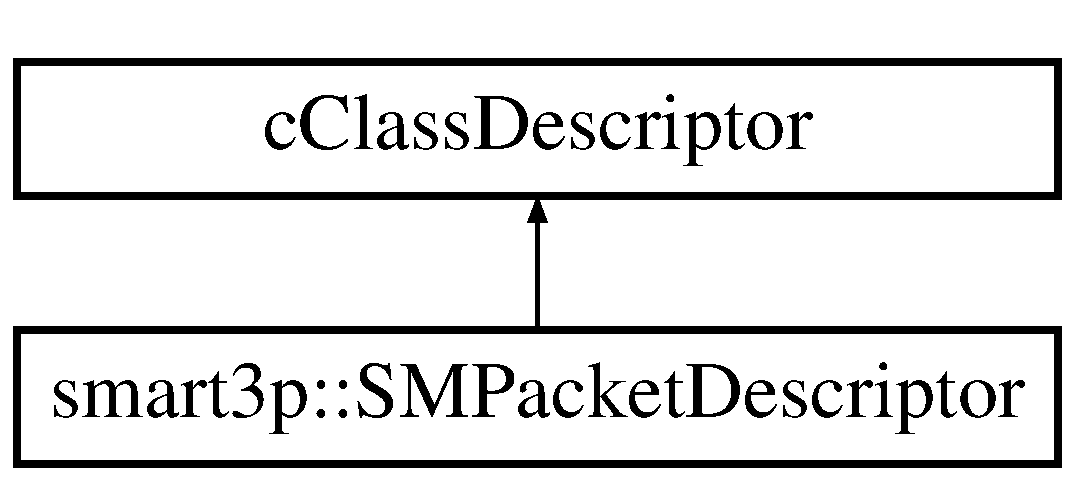
\includegraphics[height=2.000000cm]{classsmart3p_1_1SMPacketDescriptor}
\end{center}
\end{figure}
\subsection*{Public Member Functions}
\begin{DoxyCompactItemize}
\item 
\hyperlink{classsmart3p_1_1SMPacketDescriptor_ae9d949f5e29ab9f05d4cb6274dfa3200}{S\+M\+Packet\+Descriptor} ()
\item 
virtual \hyperlink{classsmart3p_1_1SMPacketDescriptor_ad0c4ce884a30eb6d2d3b318b71cd50d5}{$\sim$\+S\+M\+Packet\+Descriptor} ()
\item 
virtual bool \hyperlink{classsmart3p_1_1SMPacketDescriptor_ad6d1c39ed935c74e530518d0c08c96b1}{does\+Support} (omnetpp\+::c\+Object $\ast$obj) const override
\item 
virtual const char $\ast$$\ast$ \hyperlink{classsmart3p_1_1SMPacketDescriptor_a0b6d929f61cf3bf70beabd18b27ded6b}{get\+Property\+Names} () const override
\item 
virtual const char $\ast$ \hyperlink{classsmart3p_1_1SMPacketDescriptor_afaf28d721c4a737e995c2fa96f3980b6}{get\+Property} (const char $\ast$propertyname) const override
\item 
virtual int \hyperlink{classsmart3p_1_1SMPacketDescriptor_ae23810945a57fd295d690d93c293965c}{get\+Field\+Count} () const override
\item 
virtual const char $\ast$ \hyperlink{classsmart3p_1_1SMPacketDescriptor_a97db785c3dba89aac64029498029c49b}{get\+Field\+Name} (int field) const override
\item 
virtual int \hyperlink{classsmart3p_1_1SMPacketDescriptor_af4c4779c44e83e12d113832d241226d2}{find\+Field} (const char $\ast$field\+Name) const override
\item 
virtual unsigned int \hyperlink{classsmart3p_1_1SMPacketDescriptor_a6340a7ad7292e0479cff02e47fb40da6}{get\+Field\+Type\+Flags} (int field) const override
\item 
virtual const char $\ast$ \hyperlink{classsmart3p_1_1SMPacketDescriptor_a77f40e1520c19adb3834810ef0e1755a}{get\+Field\+Type\+String} (int field) const override
\item 
virtual const char $\ast$$\ast$ \hyperlink{classsmart3p_1_1SMPacketDescriptor_ab612eab1c11dff9714e277fe7dd1ab3c}{get\+Field\+Property\+Names} (int field) const override
\item 
virtual const char $\ast$ \hyperlink{classsmart3p_1_1SMPacketDescriptor_a6033e9cc8d7c9cfc5e6f0e0c889bf200}{get\+Field\+Property} (int field, const char $\ast$propertyname) const override
\item 
virtual int \hyperlink{classsmart3p_1_1SMPacketDescriptor_a4744e310a7b7003570a5bbd8d801fcad}{get\+Field\+Array\+Size} (void $\ast$object, int field) const override
\item 
virtual std\+::string \hyperlink{classsmart3p_1_1SMPacketDescriptor_acc1d4df999c0f9309872fe08d15393b3}{get\+Field\+Value\+As\+String} (void $\ast$object, int field, int i) const override
\item 
virtual bool \hyperlink{classsmart3p_1_1SMPacketDescriptor_a4cdbc988a0825861aba13a2ceb2db877}{set\+Field\+Value\+As\+String} (void $\ast$object, int field, int i, const char $\ast$value) const override
\item 
virtual const char $\ast$ \hyperlink{classsmart3p_1_1SMPacketDescriptor_a0ddd4481bed0f09279cc169b0315b3d3}{get\+Field\+Struct\+Name} (int field) const override
\item 
virtual void $\ast$ \hyperlink{classsmart3p_1_1SMPacketDescriptor_ac0da23c999b93f87a05b6f0009a716d6}{get\+Field\+Struct\+Value\+Pointer} (void $\ast$object, int field, int i) const override
\end{DoxyCompactItemize}


\subsection{Detailed Description}


Definition at line 284 of file S\+M\+Packet\+\_\+m.\+cc.



\subsection{Constructor \& Destructor Documentation}
\mbox{\Hypertarget{classsmart3p_1_1SMPacketDescriptor_ae9d949f5e29ab9f05d4cb6274dfa3200}\label{classsmart3p_1_1SMPacketDescriptor_ae9d949f5e29ab9f05d4cb6274dfa3200}} 
\index{smart3p\+::\+S\+M\+Packet\+Descriptor@{smart3p\+::\+S\+M\+Packet\+Descriptor}!S\+M\+Packet\+Descriptor@{S\+M\+Packet\+Descriptor}}
\index{S\+M\+Packet\+Descriptor@{S\+M\+Packet\+Descriptor}!smart3p\+::\+S\+M\+Packet\+Descriptor@{smart3p\+::\+S\+M\+Packet\+Descriptor}}
\subsubsection{\texorpdfstring{S\+M\+Packet\+Descriptor()}{SMPacketDescriptor()}}
{\footnotesize\ttfamily smart3p\+::\+S\+M\+Packet\+Descriptor\+::\+S\+M\+Packet\+Descriptor (\begin{DoxyParamCaption}{ }\end{DoxyParamCaption})}



Definition at line 313 of file S\+M\+Packet\+\_\+m.\+cc.

\mbox{\Hypertarget{classsmart3p_1_1SMPacketDescriptor_ad0c4ce884a30eb6d2d3b318b71cd50d5}\label{classsmart3p_1_1SMPacketDescriptor_ad0c4ce884a30eb6d2d3b318b71cd50d5}} 
\index{smart3p\+::\+S\+M\+Packet\+Descriptor@{smart3p\+::\+S\+M\+Packet\+Descriptor}!````~S\+M\+Packet\+Descriptor@{$\sim$\+S\+M\+Packet\+Descriptor}}
\index{````~S\+M\+Packet\+Descriptor@{$\sim$\+S\+M\+Packet\+Descriptor}!smart3p\+::\+S\+M\+Packet\+Descriptor@{smart3p\+::\+S\+M\+Packet\+Descriptor}}
\subsubsection{\texorpdfstring{$\sim$\+S\+M\+Packet\+Descriptor()}{~SMPacketDescriptor()}}
{\footnotesize\ttfamily smart3p\+::\+S\+M\+Packet\+Descriptor\+::$\sim$\+S\+M\+Packet\+Descriptor (\begin{DoxyParamCaption}{ }\end{DoxyParamCaption})\hspace{0.3cm}{\ttfamily [virtual]}}



Definition at line 318 of file S\+M\+Packet\+\_\+m.\+cc.



\subsection{Member Function Documentation}
\mbox{\Hypertarget{classsmart3p_1_1SMPacketDescriptor_ad6d1c39ed935c74e530518d0c08c96b1}\label{classsmart3p_1_1SMPacketDescriptor_ad6d1c39ed935c74e530518d0c08c96b1}} 
\index{smart3p\+::\+S\+M\+Packet\+Descriptor@{smart3p\+::\+S\+M\+Packet\+Descriptor}!does\+Support@{does\+Support}}
\index{does\+Support@{does\+Support}!smart3p\+::\+S\+M\+Packet\+Descriptor@{smart3p\+::\+S\+M\+Packet\+Descriptor}}
\subsubsection{\texorpdfstring{does\+Support()}{doesSupport()}}
{\footnotesize\ttfamily bool smart3p\+::\+S\+M\+Packet\+Descriptor\+::does\+Support (\begin{DoxyParamCaption}\item[{omnetpp\+::c\+Object $\ast$}]{obj }\end{DoxyParamCaption}) const\hspace{0.3cm}{\ttfamily [override]}, {\ttfamily [virtual]}}



Definition at line 323 of file S\+M\+Packet\+\_\+m.\+cc.

\mbox{\Hypertarget{classsmart3p_1_1SMPacketDescriptor_af4c4779c44e83e12d113832d241226d2}\label{classsmart3p_1_1SMPacketDescriptor_af4c4779c44e83e12d113832d241226d2}} 
\index{smart3p\+::\+S\+M\+Packet\+Descriptor@{smart3p\+::\+S\+M\+Packet\+Descriptor}!find\+Field@{find\+Field}}
\index{find\+Field@{find\+Field}!smart3p\+::\+S\+M\+Packet\+Descriptor@{smart3p\+::\+S\+M\+Packet\+Descriptor}}
\subsubsection{\texorpdfstring{find\+Field()}{findField()}}
{\footnotesize\ttfamily int smart3p\+::\+S\+M\+Packet\+Descriptor\+::find\+Field (\begin{DoxyParamCaption}\item[{const char $\ast$}]{field\+Name }\end{DoxyParamCaption}) const\hspace{0.3cm}{\ttfamily [override]}, {\ttfamily [virtual]}}



Definition at line 389 of file S\+M\+Packet\+\_\+m.\+cc.

\mbox{\Hypertarget{classsmart3p_1_1SMPacketDescriptor_a4744e310a7b7003570a5bbd8d801fcad}\label{classsmart3p_1_1SMPacketDescriptor_a4744e310a7b7003570a5bbd8d801fcad}} 
\index{smart3p\+::\+S\+M\+Packet\+Descriptor@{smart3p\+::\+S\+M\+Packet\+Descriptor}!get\+Field\+Array\+Size@{get\+Field\+Array\+Size}}
\index{get\+Field\+Array\+Size@{get\+Field\+Array\+Size}!smart3p\+::\+S\+M\+Packet\+Descriptor@{smart3p\+::\+S\+M\+Packet\+Descriptor}}
\subsubsection{\texorpdfstring{get\+Field\+Array\+Size()}{getFieldArraySize()}}
{\footnotesize\ttfamily int smart3p\+::\+S\+M\+Packet\+Descriptor\+::get\+Field\+Array\+Size (\begin{DoxyParamCaption}\item[{void $\ast$}]{object,  }\item[{int}]{field }\end{DoxyParamCaption}) const\hspace{0.3cm}{\ttfamily [override]}, {\ttfamily [virtual]}}



Definition at line 447 of file S\+M\+Packet\+\_\+m.\+cc.



References get\+Field\+Count().

\mbox{\Hypertarget{classsmart3p_1_1SMPacketDescriptor_ae23810945a57fd295d690d93c293965c}\label{classsmart3p_1_1SMPacketDescriptor_ae23810945a57fd295d690d93c293965c}} 
\index{smart3p\+::\+S\+M\+Packet\+Descriptor@{smart3p\+::\+S\+M\+Packet\+Descriptor}!get\+Field\+Count@{get\+Field\+Count}}
\index{get\+Field\+Count@{get\+Field\+Count}!smart3p\+::\+S\+M\+Packet\+Descriptor@{smart3p\+::\+S\+M\+Packet\+Descriptor}}
\subsubsection{\texorpdfstring{get\+Field\+Count()}{getFieldCount()}}
{\footnotesize\ttfamily int smart3p\+::\+S\+M\+Packet\+Descriptor\+::get\+Field\+Count (\begin{DoxyParamCaption}{ }\end{DoxyParamCaption}) const\hspace{0.3cm}{\ttfamily [override]}, {\ttfamily [virtual]}}



Definition at line 345 of file S\+M\+Packet\+\_\+m.\+cc.

\mbox{\Hypertarget{classsmart3p_1_1SMPacketDescriptor_a97db785c3dba89aac64029498029c49b}\label{classsmart3p_1_1SMPacketDescriptor_a97db785c3dba89aac64029498029c49b}} 
\index{smart3p\+::\+S\+M\+Packet\+Descriptor@{smart3p\+::\+S\+M\+Packet\+Descriptor}!get\+Field\+Name@{get\+Field\+Name}}
\index{get\+Field\+Name@{get\+Field\+Name}!smart3p\+::\+S\+M\+Packet\+Descriptor@{smart3p\+::\+S\+M\+Packet\+Descriptor}}
\subsubsection{\texorpdfstring{get\+Field\+Name()}{getFieldName()}}
{\footnotesize\ttfamily const char $\ast$ smart3p\+::\+S\+M\+Packet\+Descriptor\+::get\+Field\+Name (\begin{DoxyParamCaption}\item[{int}]{field }\end{DoxyParamCaption}) const\hspace{0.3cm}{\ttfamily [override]}, {\ttfamily [virtual]}}



Definition at line 370 of file S\+M\+Packet\+\_\+m.\+cc.



References get\+Field\+Count().

\mbox{\Hypertarget{classsmart3p_1_1SMPacketDescriptor_a6033e9cc8d7c9cfc5e6f0e0c889bf200}\label{classsmart3p_1_1SMPacketDescriptor_a6033e9cc8d7c9cfc5e6f0e0c889bf200}} 
\index{smart3p\+::\+S\+M\+Packet\+Descriptor@{smart3p\+::\+S\+M\+Packet\+Descriptor}!get\+Field\+Property@{get\+Field\+Property}}
\index{get\+Field\+Property@{get\+Field\+Property}!smart3p\+::\+S\+M\+Packet\+Descriptor@{smart3p\+::\+S\+M\+Packet\+Descriptor}}
\subsubsection{\texorpdfstring{get\+Field\+Property()}{getFieldProperty()}}
{\footnotesize\ttfamily const char $\ast$ smart3p\+::\+S\+M\+Packet\+Descriptor\+::get\+Field\+Property (\begin{DoxyParamCaption}\item[{int}]{field,  }\item[{const char $\ast$}]{propertyname }\end{DoxyParamCaption}) const\hspace{0.3cm}{\ttfamily [override]}, {\ttfamily [virtual]}}



Definition at line 434 of file S\+M\+Packet\+\_\+m.\+cc.



References get\+Field\+Count().

\mbox{\Hypertarget{classsmart3p_1_1SMPacketDescriptor_ab612eab1c11dff9714e277fe7dd1ab3c}\label{classsmart3p_1_1SMPacketDescriptor_ab612eab1c11dff9714e277fe7dd1ab3c}} 
\index{smart3p\+::\+S\+M\+Packet\+Descriptor@{smart3p\+::\+S\+M\+Packet\+Descriptor}!get\+Field\+Property\+Names@{get\+Field\+Property\+Names}}
\index{get\+Field\+Property\+Names@{get\+Field\+Property\+Names}!smart3p\+::\+S\+M\+Packet\+Descriptor@{smart3p\+::\+S\+M\+Packet\+Descriptor}}
\subsubsection{\texorpdfstring{get\+Field\+Property\+Names()}{getFieldPropertyNames()}}
{\footnotesize\ttfamily const char $\ast$$\ast$ smart3p\+::\+S\+M\+Packet\+Descriptor\+::get\+Field\+Property\+Names (\begin{DoxyParamCaption}\item[{int}]{field }\end{DoxyParamCaption}) const\hspace{0.3cm}{\ttfamily [override]}, {\ttfamily [virtual]}}



Definition at line 421 of file S\+M\+Packet\+\_\+m.\+cc.



References get\+Field\+Count().

\mbox{\Hypertarget{classsmart3p_1_1SMPacketDescriptor_a0ddd4481bed0f09279cc169b0315b3d3}\label{classsmart3p_1_1SMPacketDescriptor_a0ddd4481bed0f09279cc169b0315b3d3}} 
\index{smart3p\+::\+S\+M\+Packet\+Descriptor@{smart3p\+::\+S\+M\+Packet\+Descriptor}!get\+Field\+Struct\+Name@{get\+Field\+Struct\+Name}}
\index{get\+Field\+Struct\+Name@{get\+Field\+Struct\+Name}!smart3p\+::\+S\+M\+Packet\+Descriptor@{smart3p\+::\+S\+M\+Packet\+Descriptor}}
\subsubsection{\texorpdfstring{get\+Field\+Struct\+Name()}{getFieldStructName()}}
{\footnotesize\ttfamily const char $\ast$ smart3p\+::\+S\+M\+Packet\+Descriptor\+::get\+Field\+Struct\+Name (\begin{DoxyParamCaption}\item[{int}]{field }\end{DoxyParamCaption}) const\hspace{0.3cm}{\ttfamily [override]}, {\ttfamily [virtual]}}



Definition at line 501 of file S\+M\+Packet\+\_\+m.\+cc.



References get\+Field\+Count().

\mbox{\Hypertarget{classsmart3p_1_1SMPacketDescriptor_ac0da23c999b93f87a05b6f0009a716d6}\label{classsmart3p_1_1SMPacketDescriptor_ac0da23c999b93f87a05b6f0009a716d6}} 
\index{smart3p\+::\+S\+M\+Packet\+Descriptor@{smart3p\+::\+S\+M\+Packet\+Descriptor}!get\+Field\+Struct\+Value\+Pointer@{get\+Field\+Struct\+Value\+Pointer}}
\index{get\+Field\+Struct\+Value\+Pointer@{get\+Field\+Struct\+Value\+Pointer}!smart3p\+::\+S\+M\+Packet\+Descriptor@{smart3p\+::\+S\+M\+Packet\+Descriptor}}
\subsubsection{\texorpdfstring{get\+Field\+Struct\+Value\+Pointer()}{getFieldStructValuePointer()}}
{\footnotesize\ttfamily void $\ast$ smart3p\+::\+S\+M\+Packet\+Descriptor\+::get\+Field\+Struct\+Value\+Pointer (\begin{DoxyParamCaption}\item[{void $\ast$}]{object,  }\item[{int}]{field,  }\item[{int}]{i }\end{DoxyParamCaption}) const\hspace{0.3cm}{\ttfamily [override]}, {\ttfamily [virtual]}}



Definition at line 514 of file S\+M\+Packet\+\_\+m.\+cc.



References get\+Field\+Count().

\mbox{\Hypertarget{classsmart3p_1_1SMPacketDescriptor_a6340a7ad7292e0479cff02e47fb40da6}\label{classsmart3p_1_1SMPacketDescriptor_a6340a7ad7292e0479cff02e47fb40da6}} 
\index{smart3p\+::\+S\+M\+Packet\+Descriptor@{smart3p\+::\+S\+M\+Packet\+Descriptor}!get\+Field\+Type\+Flags@{get\+Field\+Type\+Flags}}
\index{get\+Field\+Type\+Flags@{get\+Field\+Type\+Flags}!smart3p\+::\+S\+M\+Packet\+Descriptor@{smart3p\+::\+S\+M\+Packet\+Descriptor}}
\subsubsection{\texorpdfstring{get\+Field\+Type\+Flags()}{getFieldTypeFlags()}}
{\footnotesize\ttfamily unsigned int smart3p\+::\+S\+M\+Packet\+Descriptor\+::get\+Field\+Type\+Flags (\begin{DoxyParamCaption}\item[{int}]{field }\end{DoxyParamCaption}) const\hspace{0.3cm}{\ttfamily [override]}, {\ttfamily [virtual]}}



Definition at line 351 of file S\+M\+Packet\+\_\+m.\+cc.



References get\+Field\+Count().

\mbox{\Hypertarget{classsmart3p_1_1SMPacketDescriptor_a77f40e1520c19adb3834810ef0e1755a}\label{classsmart3p_1_1SMPacketDescriptor_a77f40e1520c19adb3834810ef0e1755a}} 
\index{smart3p\+::\+S\+M\+Packet\+Descriptor@{smart3p\+::\+S\+M\+Packet\+Descriptor}!get\+Field\+Type\+String@{get\+Field\+Type\+String}}
\index{get\+Field\+Type\+String@{get\+Field\+Type\+String}!smart3p\+::\+S\+M\+Packet\+Descriptor@{smart3p\+::\+S\+M\+Packet\+Descriptor}}
\subsubsection{\texorpdfstring{get\+Field\+Type\+String()}{getFieldTypeString()}}
{\footnotesize\ttfamily const char $\ast$ smart3p\+::\+S\+M\+Packet\+Descriptor\+::get\+Field\+Type\+String (\begin{DoxyParamCaption}\item[{int}]{field }\end{DoxyParamCaption}) const\hspace{0.3cm}{\ttfamily [override]}, {\ttfamily [virtual]}}



Definition at line 402 of file S\+M\+Packet\+\_\+m.\+cc.



References get\+Field\+Count().

\mbox{\Hypertarget{classsmart3p_1_1SMPacketDescriptor_acc1d4df999c0f9309872fe08d15393b3}\label{classsmart3p_1_1SMPacketDescriptor_acc1d4df999c0f9309872fe08d15393b3}} 
\index{smart3p\+::\+S\+M\+Packet\+Descriptor@{smart3p\+::\+S\+M\+Packet\+Descriptor}!get\+Field\+Value\+As\+String@{get\+Field\+Value\+As\+String}}
\index{get\+Field\+Value\+As\+String@{get\+Field\+Value\+As\+String}!smart3p\+::\+S\+M\+Packet\+Descriptor@{smart3p\+::\+S\+M\+Packet\+Descriptor}}
\subsubsection{\texorpdfstring{get\+Field\+Value\+As\+String()}{getFieldValueAsString()}}
{\footnotesize\ttfamily std\+::string smart3p\+::\+S\+M\+Packet\+Descriptor\+::get\+Field\+Value\+As\+String (\begin{DoxyParamCaption}\item[{void $\ast$}]{object,  }\item[{int}]{field,  }\item[{int}]{i }\end{DoxyParamCaption}) const\hspace{0.3cm}{\ttfamily [override]}, {\ttfamily [virtual]}}



Definition at line 461 of file S\+M\+Packet\+\_\+m.\+cc.



References smart3p\+::\+S\+M\+Packet\+::get\+Coll\+Gate\+I\+D(), smart3p\+::\+S\+M\+Packet\+::get\+Extra\+Info(), smart3p\+::\+S\+M\+Packet\+::get\+Extra\+Info\+Size(), get\+Field\+Count(), smart3p\+::\+S\+M\+Packet\+::get\+Id(), smart3p\+::\+S\+M\+Packet\+::get\+Sm\+Gate\+I\+D(), and smart3p\+::\+S\+M\+Packet\+::get\+Value().

\mbox{\Hypertarget{classsmart3p_1_1SMPacketDescriptor_afaf28d721c4a737e995c2fa96f3980b6}\label{classsmart3p_1_1SMPacketDescriptor_afaf28d721c4a737e995c2fa96f3980b6}} 
\index{smart3p\+::\+S\+M\+Packet\+Descriptor@{smart3p\+::\+S\+M\+Packet\+Descriptor}!get\+Property@{get\+Property}}
\index{get\+Property@{get\+Property}!smart3p\+::\+S\+M\+Packet\+Descriptor@{smart3p\+::\+S\+M\+Packet\+Descriptor}}
\subsubsection{\texorpdfstring{get\+Property()}{getProperty()}}
{\footnotesize\ttfamily const char $\ast$ smart3p\+::\+S\+M\+Packet\+Descriptor\+::get\+Property (\begin{DoxyParamCaption}\item[{const char $\ast$}]{propertyname }\end{DoxyParamCaption}) const\hspace{0.3cm}{\ttfamily [override]}, {\ttfamily [virtual]}}



Definition at line 339 of file S\+M\+Packet\+\_\+m.\+cc.

\mbox{\Hypertarget{classsmart3p_1_1SMPacketDescriptor_a0b6d929f61cf3bf70beabd18b27ded6b}\label{classsmart3p_1_1SMPacketDescriptor_a0b6d929f61cf3bf70beabd18b27ded6b}} 
\index{smart3p\+::\+S\+M\+Packet\+Descriptor@{smart3p\+::\+S\+M\+Packet\+Descriptor}!get\+Property\+Names@{get\+Property\+Names}}
\index{get\+Property\+Names@{get\+Property\+Names}!smart3p\+::\+S\+M\+Packet\+Descriptor@{smart3p\+::\+S\+M\+Packet\+Descriptor}}
\subsubsection{\texorpdfstring{get\+Property\+Names()}{getPropertyNames()}}
{\footnotesize\ttfamily const char $\ast$$\ast$ smart3p\+::\+S\+M\+Packet\+Descriptor\+::get\+Property\+Names (\begin{DoxyParamCaption}{ }\end{DoxyParamCaption}) const\hspace{0.3cm}{\ttfamily [override]}, {\ttfamily [virtual]}}



Definition at line 328 of file S\+M\+Packet\+\_\+m.\+cc.

\mbox{\Hypertarget{classsmart3p_1_1SMPacketDescriptor_a4cdbc988a0825861aba13a2ceb2db877}\label{classsmart3p_1_1SMPacketDescriptor_a4cdbc988a0825861aba13a2ceb2db877}} 
\index{smart3p\+::\+S\+M\+Packet\+Descriptor@{smart3p\+::\+S\+M\+Packet\+Descriptor}!set\+Field\+Value\+As\+String@{set\+Field\+Value\+As\+String}}
\index{set\+Field\+Value\+As\+String@{set\+Field\+Value\+As\+String}!smart3p\+::\+S\+M\+Packet\+Descriptor@{smart3p\+::\+S\+M\+Packet\+Descriptor}}
\subsubsection{\texorpdfstring{set\+Field\+Value\+As\+String()}{setFieldValueAsString()}}
{\footnotesize\ttfamily bool smart3p\+::\+S\+M\+Packet\+Descriptor\+::set\+Field\+Value\+As\+String (\begin{DoxyParamCaption}\item[{void $\ast$}]{object,  }\item[{int}]{field,  }\item[{int}]{i,  }\item[{const char $\ast$}]{value }\end{DoxyParamCaption}) const\hspace{0.3cm}{\ttfamily [override]}, {\ttfamily [virtual]}}



Definition at line 481 of file S\+M\+Packet\+\_\+m.\+cc.



References get\+Field\+Count(), smart3p\+::\+S\+M\+Packet\+::set\+Coll\+Gate\+I\+D(), smart3p\+::\+S\+M\+Packet\+::set\+Extra\+Info(), smart3p\+::\+S\+M\+Packet\+::set\+Extra\+Info\+Size(), smart3p\+::\+S\+M\+Packet\+::set\+Id(), smart3p\+::\+S\+M\+Packet\+::set\+Sm\+Gate\+I\+D(), and smart3p\+::\+S\+M\+Packet\+::set\+Value().



The documentation for this class was generated from the following file\+:\begin{DoxyCompactItemize}
\item 
src/\hyperlink{SMPacket__m_8cc}{S\+M\+Packet\+\_\+m.\+cc}\end{DoxyCompactItemize}

\hypertarget{classSMImp_1_1TrustedParty}{}\section{S\+M\+Imp\+:\+:Trusted\+Party Class Reference}
\label{classSMImp_1_1TrustedParty}\index{S\+M\+Imp\+::\+Trusted\+Party@{S\+M\+Imp\+::\+Trusted\+Party}}


Trusted Third Party protocol implementation.  




{\ttfamily \#include $<$Trusted\+Party.\+h$>$}

Inheritance diagram for S\+M\+Imp\+:\+:Trusted\+Party\+:\begin{figure}[H]
\begin{center}
\leavevmode
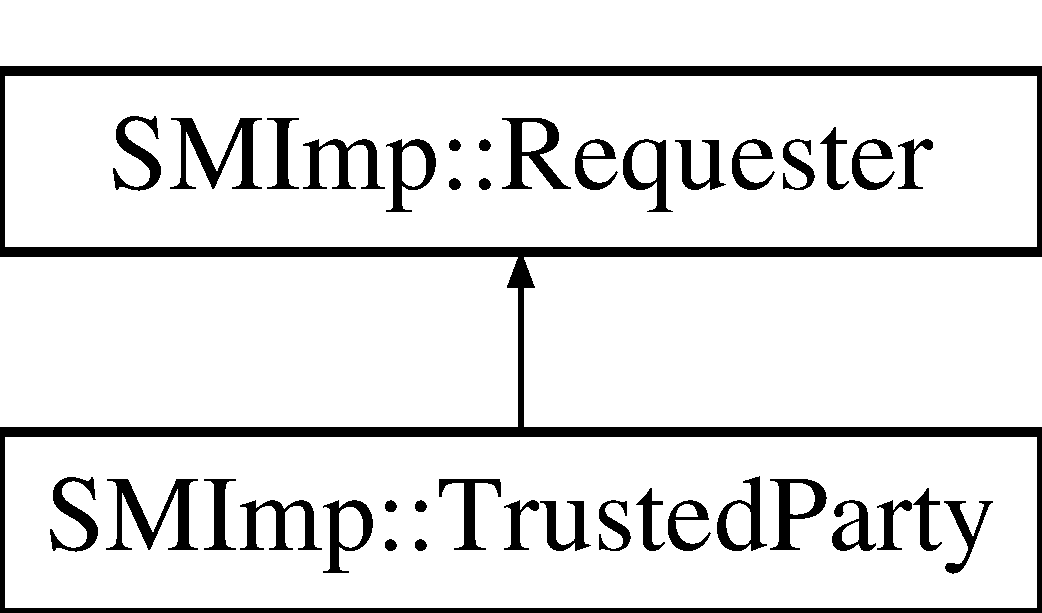
\includegraphics[height=2.000000cm]{classSMImp_1_1TrustedParty}
\end{center}
\end{figure}
\subsection*{Public Member Functions}
\begin{DoxyCompactItemize}
\item 
\hyperlink{classSMImp_1_1TrustedParty_aec9d85830faf563a55c67b637b38bc0a}{Trusted\+Party} (Integer)
\item 
\hyperlink{classSMImp_1_1TrustedParty_ad48b557601e6793a80b9b4b42d586da1}{Trusted\+Party} (Integer, \hyperlink{classTTPAdapter}{T\+T\+P\+Adapter} $\ast$)
\item 
virtual \hyperlink{classSMImp_1_1TrustedParty_a93dd8343a752486f8a47691b429ad6a3}{$\sim$\+Trusted\+Party} ()
\item 
char $\ast$ \hyperlink{classSMImp_1_1TrustedParty_ab15efea2439c964eec1f0cdae82843ac}{get\+Message} ()
\item 
void \hyperlink{classSMImp_1_1TrustedParty_adc01721f3200888877174376a5b2464f}{register\+SM} (int)
\item 
void \hyperlink{classSMImp_1_1TrustedParty_aa8343369b112c07a86ab42a9ee64228b}{add\+Data\+To\+SM} (int \hyperlink{classSMImp_1_1Requester_a16911083f2e3fc903ed3e6e7ca2a58b1}{id}, Integer $\ast$data)
\item 
\hyperlink{classList}{List}$<$ Integer $>$ $\ast$ \hyperlink{classSMImp_1_1TrustedParty_a979f9046e92d8be8fd97b1f3bc92dcd0}{get\+SM} (int \hyperlink{classSMImp_1_1Requester_a16911083f2e3fc903ed3e6e7ca2a58b1}{id})
\item 
\hyperlink{classList}{List}$<$ Integer $>$ $\ast$ \hyperlink{classSMImp_1_1TrustedParty_a8c0452d2d9842a1c24ebf6dffac9529a}{get\+Random\+SM} ()
\item 
\hyperlink{classIterator}{Iterator}$<$ \hyperlink{classList}{List}$<$ Integer $>$ $>$ $\ast$ \hyperlink{classSMImp_1_1TrustedParty_a01cbd1bd12aaca134b0730bd2a6eb933}{get\+S\+M\+Iterator} ()
\item 
\hyperlink{structSMImp_1_1Packet}{Packet} \hyperlink{classSMImp_1_1TrustedParty_a34334b73f543168b6270a8bb36de04c3}{confirm\+Session} (Integer req, Integer sm\+Id, \hyperlink{structSMImp_1_1Key}{Key} sm\+Key)
\item 
bool \hyperlink{classSMImp_1_1TrustedParty_a889787f394517703c1d9d2dfd9b9ff9b}{recieve\+H\+M\+AC} (Integer length, Integer c1, Integer c2, Integer sm\+Id, \hyperlink{structSMImp_1_1Key}{Key} sm\+Key, Integer r)
\item 
Integer \hyperlink{classSMImp_1_1TrustedParty_ab812aac2ce15865341874f1cd9550ba4}{recieve\+Data} (Integer length, Integer c1, Integer c2, Integer sm\+Id, Integer time\+Stamp)
\end{DoxyCompactItemize}
\subsection*{Additional Inherited Members}


\subsection{Detailed Description}
Trusted Third Party protocol implementation. 

Most variables have been named after their respective names given in the original research paper available \href{https://www.researchgate.net/publication/305077004_Secure_and_efficient_protection_of_consumer_privacy_in_Advanced_Metering_Infrastructure_supporting_fine-grained_data_analysis}{\tt here}. See section 5 (Page 7) for the beginning of the protocol implementation. 

Definition at line 15 of file Trusted\+Party.\+h.



\subsection{Constructor \& Destructor Documentation}
\mbox{\Hypertarget{classSMImp_1_1TrustedParty_aec9d85830faf563a55c67b637b38bc0a}\label{classSMImp_1_1TrustedParty_aec9d85830faf563a55c67b637b38bc0a}} 
\index{S\+M\+Imp\+::\+Trusted\+Party@{S\+M\+Imp\+::\+Trusted\+Party}!Trusted\+Party@{Trusted\+Party}}
\index{Trusted\+Party@{Trusted\+Party}!S\+M\+Imp\+::\+Trusted\+Party@{S\+M\+Imp\+::\+Trusted\+Party}}
\subsubsection{\texorpdfstring{Trusted\+Party()}{TrustedParty()}\hspace{0.1cm}{\footnotesize\ttfamily [1/2]}}
{\footnotesize\ttfamily S\+M\+Imp\+::\+Trusted\+Party\+::\+Trusted\+Party (\begin{DoxyParamCaption}\item[{Integer}]{i }\end{DoxyParamCaption})}



Definition at line 16 of file Trusted\+Party.\+cc.

\mbox{\Hypertarget{classSMImp_1_1TrustedParty_ad48b557601e6793a80b9b4b42d586da1}\label{classSMImp_1_1TrustedParty_ad48b557601e6793a80b9b4b42d586da1}} 
\index{S\+M\+Imp\+::\+Trusted\+Party@{S\+M\+Imp\+::\+Trusted\+Party}!Trusted\+Party@{Trusted\+Party}}
\index{Trusted\+Party@{Trusted\+Party}!S\+M\+Imp\+::\+Trusted\+Party@{S\+M\+Imp\+::\+Trusted\+Party}}
\subsubsection{\texorpdfstring{Trusted\+Party()}{TrustedParty()}\hspace{0.1cm}{\footnotesize\ttfamily [2/2]}}
{\footnotesize\ttfamily S\+M\+Imp\+::\+Trusted\+Party\+::\+Trusted\+Party (\begin{DoxyParamCaption}\item[{Integer}]{i,  }\item[{\hyperlink{classTTPAdapter}{T\+T\+P\+Adapter} $\ast$}]{o }\end{DoxyParamCaption})}

For debugging. 

Definition at line 9 of file Trusted\+Party.\+cc.

\mbox{\Hypertarget{classSMImp_1_1TrustedParty_a93dd8343a752486f8a47691b429ad6a3}\label{classSMImp_1_1TrustedParty_a93dd8343a752486f8a47691b429ad6a3}} 
\index{S\+M\+Imp\+::\+Trusted\+Party@{S\+M\+Imp\+::\+Trusted\+Party}!````~Trusted\+Party@{$\sim$\+Trusted\+Party}}
\index{````~Trusted\+Party@{$\sim$\+Trusted\+Party}!S\+M\+Imp\+::\+Trusted\+Party@{S\+M\+Imp\+::\+Trusted\+Party}}
\subsubsection{\texorpdfstring{$\sim$\+Trusted\+Party()}{~TrustedParty()}}
{\footnotesize\ttfamily S\+M\+Imp\+::\+Trusted\+Party\+::$\sim$\+Trusted\+Party (\begin{DoxyParamCaption}{ }\end{DoxyParamCaption})\hspace{0.3cm}{\ttfamily [virtual]}}



Definition at line 23 of file Trusted\+Party.\+cc.



\subsection{Member Function Documentation}
\mbox{\Hypertarget{classSMImp_1_1TrustedParty_aa8343369b112c07a86ab42a9ee64228b}\label{classSMImp_1_1TrustedParty_aa8343369b112c07a86ab42a9ee64228b}} 
\index{S\+M\+Imp\+::\+Trusted\+Party@{S\+M\+Imp\+::\+Trusted\+Party}!add\+Data\+To\+SM@{add\+Data\+To\+SM}}
\index{add\+Data\+To\+SM@{add\+Data\+To\+SM}!S\+M\+Imp\+::\+Trusted\+Party@{S\+M\+Imp\+::\+Trusted\+Party}}
\subsubsection{\texorpdfstring{add\+Data\+To\+S\+M()}{addDataToSM()}}
{\footnotesize\ttfamily void S\+M\+Imp\+::\+Trusted\+Party\+::add\+Data\+To\+SM (\begin{DoxyParamCaption}\item[{int}]{id,  }\item[{Integer $\ast$}]{data }\end{DoxyParamCaption})}

Adds arbitrary data to the local Smart Meter representation identified by id. 
\begin{DoxyParams}{Parameters}
{\em id} & ID of the Smart Meter to add data to. \\
\hline
{\em data} & Data to add to the local Smart Meter representation. \\
\hline
\end{DoxyParams}


Definition at line 49 of file Trusted\+Party.\+cc.



References List$<$ T $>$\+::add(), List$<$ T $>$\+::get(), and List$<$ T $>$\+::size().

\mbox{\Hypertarget{classSMImp_1_1TrustedParty_a34334b73f543168b6270a8bb36de04c3}\label{classSMImp_1_1TrustedParty_a34334b73f543168b6270a8bb36de04c3}} 
\index{S\+M\+Imp\+::\+Trusted\+Party@{S\+M\+Imp\+::\+Trusted\+Party}!confirm\+Session@{confirm\+Session}}
\index{confirm\+Session@{confirm\+Session}!S\+M\+Imp\+::\+Trusted\+Party@{S\+M\+Imp\+::\+Trusted\+Party}}
\subsubsection{\texorpdfstring{confirm\+Session()}{confirmSession()}}
{\footnotesize\ttfamily \hyperlink{structSMImp_1_1Packet}{Packet} S\+M\+Imp\+::\+Trusted\+Party\+::confirm\+Session (\begin{DoxyParamCaption}\item[{Integer}]{req,  }\item[{Integer}]{sm\+Id,  }\item[{\hyperlink{structSMImp_1_1Key}{Key}}]{sm\+Key }\end{DoxyParamCaption})}

Recieves session key exchange data from Smart Meter. 
\begin{DoxyParams}{Parameters}
{\em req} & Shared secret R for use with future encryption. \\
\hline
{\em sm\+Id} & ID (anonymous) for identifying the Smart Meter (used by \hyperlink{classSMImp_1_1TrustedParty_a979f9046e92d8be8fd97b1f3bc92dcd0}{get\+S\+M(int id)}). \\
\hline
{\em sm\+Key} & Public key of the Smart Meter. \\
\hline
\end{DoxyParams}
\begin{DoxyReturn}{Returns}
\hyperlink{structSMImp_1_1Packet}{Packet} to be sent back to the Smart Meter. 
\end{DoxyReturn}


Definition at line 70 of file Trusted\+Party.\+cc.



References List$<$ T $>$\+::add(), S\+M\+Imp\+::\+H\+M\+A\+C\+Payload\+::c1, S\+M\+Imp\+::\+H\+M\+A\+C\+Payload\+::c2, S\+M\+Imp\+::\+Packet\+::dest, S\+M\+Imp\+::\+Master\+Key\+::g, List$<$ T $>$\+::get(), S\+M\+Imp\+::\+H\+M\+A\+C\+Payload\+::hmac, S\+M\+Imp\+::\+Requester\+::id, S\+M\+Imp\+::\+H\+M\+A\+C\+Payload\+::id, S\+M\+Imp\+::\+Master\+Key\+::p, S\+M\+Imp\+::\+Requester\+::params, S\+M\+Imp\+::\+Key\+::partial, S\+M\+Imp\+::\+Key\+::piece, S\+M\+Imp\+::\+Packet\+::pl, S\+M\+Imp\+::\+Requester\+::rng, S\+M\+Imp\+::\+Requester\+::shaone, S\+M\+Imp\+::\+H\+M\+A\+C\+Payload\+::time\+Stamp, and S\+M\+Imp\+::\+Master\+Key\+::x.

\mbox{\Hypertarget{classSMImp_1_1TrustedParty_ab15efea2439c964eec1f0cdae82843ac}\label{classSMImp_1_1TrustedParty_ab15efea2439c964eec1f0cdae82843ac}} 
\index{S\+M\+Imp\+::\+Trusted\+Party@{S\+M\+Imp\+::\+Trusted\+Party}!get\+Message@{get\+Message}}
\index{get\+Message@{get\+Message}!S\+M\+Imp\+::\+Trusted\+Party@{S\+M\+Imp\+::\+Trusted\+Party}}
\subsubsection{\texorpdfstring{get\+Message()}{getMessage()}}
{\footnotesize\ttfamily char$\ast$ S\+M\+Imp\+::\+Trusted\+Party\+::get\+Message (\begin{DoxyParamCaption}{ }\end{DoxyParamCaption})}

Helper function for the \hyperlink{classAdapter}{Adapter} to queuery the current message. \begin{DoxyReturn}{Returns}
message 
\end{DoxyReturn}
\begin{DoxySeeAlso}{See also}
message. 
\end{DoxySeeAlso}
\mbox{\Hypertarget{classSMImp_1_1TrustedParty_a8c0452d2d9842a1c24ebf6dffac9529a}\label{classSMImp_1_1TrustedParty_a8c0452d2d9842a1c24ebf6dffac9529a}} 
\index{S\+M\+Imp\+::\+Trusted\+Party@{S\+M\+Imp\+::\+Trusted\+Party}!get\+Random\+SM@{get\+Random\+SM}}
\index{get\+Random\+SM@{get\+Random\+SM}!S\+M\+Imp\+::\+Trusted\+Party@{S\+M\+Imp\+::\+Trusted\+Party}}
\subsubsection{\texorpdfstring{get\+Random\+S\+M()}{getRandomSM()}}
{\footnotesize\ttfamily \hyperlink{classList}{List}$<$ Integer $>$ $\ast$ S\+M\+Imp\+::\+Trusted\+Party\+::get\+Random\+SM (\begin{DoxyParamCaption}{ }\end{DoxyParamCaption})}

Gets a random Smart Meter representation for use with session key exchange. \begin{DoxyReturn}{Returns}
Local Smart Meter representation of arbitrary data. 
\end{DoxyReturn}


Definition at line 60 of file Trusted\+Party.\+cc.



References List$<$ T $>$\+::get\+Random().

\mbox{\Hypertarget{classSMImp_1_1TrustedParty_a979f9046e92d8be8fd97b1f3bc92dcd0}\label{classSMImp_1_1TrustedParty_a979f9046e92d8be8fd97b1f3bc92dcd0}} 
\index{S\+M\+Imp\+::\+Trusted\+Party@{S\+M\+Imp\+::\+Trusted\+Party}!get\+SM@{get\+SM}}
\index{get\+SM@{get\+SM}!S\+M\+Imp\+::\+Trusted\+Party@{S\+M\+Imp\+::\+Trusted\+Party}}
\subsubsection{\texorpdfstring{get\+S\+M()}{getSM()}}
{\footnotesize\ttfamily \hyperlink{classList}{List}$<$ Integer $>$ $\ast$ S\+M\+Imp\+::\+Trusted\+Party\+::get\+SM (\begin{DoxyParamCaption}\item[{int}]{id }\end{DoxyParamCaption})}

Gets local Smart Meter representation by ID 
\begin{DoxyParams}{Parameters}
{\em id} & Smart Meter ID to retrieve. \\
\hline
\end{DoxyParams}
\begin{DoxyReturn}{Returns}
Local Smart Meter representation of arbitrary data. 
\end{DoxyReturn}


Definition at line 55 of file Trusted\+Party.\+cc.



References List$<$ T $>$\+::get().

\mbox{\Hypertarget{classSMImp_1_1TrustedParty_a01cbd1bd12aaca134b0730bd2a6eb933}\label{classSMImp_1_1TrustedParty_a01cbd1bd12aaca134b0730bd2a6eb933}} 
\index{S\+M\+Imp\+::\+Trusted\+Party@{S\+M\+Imp\+::\+Trusted\+Party}!get\+S\+M\+Iterator@{get\+S\+M\+Iterator}}
\index{get\+S\+M\+Iterator@{get\+S\+M\+Iterator}!S\+M\+Imp\+::\+Trusted\+Party@{S\+M\+Imp\+::\+Trusted\+Party}}
\subsubsection{\texorpdfstring{get\+S\+M\+Iterator()}{getSMIterator()}}
{\footnotesize\ttfamily \hyperlink{classIterator}{Iterator}$<$ \hyperlink{classList}{List}$<$ Integer $>$ $>$ $\ast$ S\+M\+Imp\+::\+Trusted\+Party\+::get\+S\+M\+Iterator (\begin{DoxyParamCaption}{ }\end{DoxyParamCaption})}

Get an iterator to iterate over all available Smart Meters. \begin{DoxyReturn}{Returns}
\hyperlink{classIterator}{Iterator} to iterate with. 
\end{DoxyReturn}


Definition at line 65 of file Trusted\+Party.\+cc.



References List$<$ T $>$\+::iterator().

\mbox{\Hypertarget{classSMImp_1_1TrustedParty_ab812aac2ce15865341874f1cd9550ba4}\label{classSMImp_1_1TrustedParty_ab812aac2ce15865341874f1cd9550ba4}} 
\index{S\+M\+Imp\+::\+Trusted\+Party@{S\+M\+Imp\+::\+Trusted\+Party}!recieve\+Data@{recieve\+Data}}
\index{recieve\+Data@{recieve\+Data}!S\+M\+Imp\+::\+Trusted\+Party@{S\+M\+Imp\+::\+Trusted\+Party}}
\subsubsection{\texorpdfstring{recieve\+Data()}{recieveData()}}
{\footnotesize\ttfamily Integer S\+M\+Imp\+::\+Trusted\+Party\+::recieve\+Data (\begin{DoxyParamCaption}\item[{Integer}]{length,  }\item[{Integer}]{c1,  }\item[{Integer}]{c2,  }\item[{Integer}]{sm\+Id,  }\item[{Integer}]{time\+Stamp }\end{DoxyParamCaption})}

Recieve, verify and decrypt energy usage data. 
\begin{DoxyParams}{Parameters}
{\em length} & Length of the message (unused as it is equivalent to the sum of the lengths of c1 and c2) \\
\hline
{\em c1} & Part 1 of the encrypted energy usage data. \\
\hline
{\em c2} & Part 2 of the encrypted energy usage data. \\
\hline
{\em sm\+Id} & ID (anonymous) of the Smart Meter the data originated from. \\
\hline
{\em time\+Stamp} & Timestamp of the data. \\
\hline
\end{DoxyParams}
\begin{DoxyReturn}{Returns}
-\/1 if failed to verify. Any other value is the byte-\/encoded string of the data, see \hyperlink{classTTPAdapter_ab69604de63c3f769a10ec33168611274}{T\+T\+P\+Adapter\+::process\+Data\+From\+S\+M(omnetpp\+::c\+Message$\ast$ msg)} 
\end{DoxyReturn}


Definition at line 131 of file Trusted\+Party.\+cc.



References D\+E\+B\+UG, S\+M\+Imp\+::\+Master\+Key\+::g, List$<$ T $>$\+::get(), S\+M\+Imp\+::\+Master\+Key\+::p, S\+M\+Imp\+::\+Requester\+::params, and S\+M\+Imp\+::\+Requester\+::session\+Key.

\mbox{\Hypertarget{classSMImp_1_1TrustedParty_a889787f394517703c1d9d2dfd9b9ff9b}\label{classSMImp_1_1TrustedParty_a889787f394517703c1d9d2dfd9b9ff9b}} 
\index{S\+M\+Imp\+::\+Trusted\+Party@{S\+M\+Imp\+::\+Trusted\+Party}!recieve\+H\+M\+AC@{recieve\+H\+M\+AC}}
\index{recieve\+H\+M\+AC@{recieve\+H\+M\+AC}!S\+M\+Imp\+::\+Trusted\+Party@{S\+M\+Imp\+::\+Trusted\+Party}}
\subsubsection{\texorpdfstring{recieve\+H\+M\+A\+C()}{recieveHMAC()}}
{\footnotesize\ttfamily bool S\+M\+Imp\+::\+Trusted\+Party\+::recieve\+H\+M\+AC (\begin{DoxyParamCaption}\item[{Integer}]{length,  }\item[{Integer}]{c1,  }\item[{Integer}]{c2,  }\item[{Integer}]{sm\+Id,  }\item[{\hyperlink{structSMImp_1_1Key}{Key}}]{sm\+Key,  }\item[{Integer}]{r }\end{DoxyParamCaption})}

Finishes the Session \hyperlink{structSMImp_1_1Key}{Key} exchange phase for the Trusted Third Party. 
\begin{DoxyParams}{Parameters}
{\em length} & Total length of the session key. Unlike \hyperlink{classSMImp_1_1TrustedParty_a889787f394517703c1d9d2dfd9b9ff9b}{recieve\+H\+M\+A\+C(\+Integer length, Integer c1, Integer c2, Integer id, Key sm\+Key, Integer r)} the sum of the lengths of c1 and c2 may be less than the length of the entire session key. \\
\hline
{\em c1} & Part 1 of the encrypted Session \hyperlink{structSMImp_1_1Key}{Key}. \\
\hline
{\em c2} & Part 2 of the encrypted Session \hyperlink{structSMImp_1_1Key}{Key}. \\
\hline
{\em sm\+Id} & ID (anonymous) of the Smart Meter the Session \hyperlink{structSMImp_1_1Key}{Key} originated from. \\
\hline
{\em sm\+Key} & Public key of Smart Meter. \\
\hline
{\em r} & shared-\/secret used for message verification. \\
\hline
\end{DoxyParams}
\begin{DoxyReturn}{Returns}
Returns true if session key passed verification, false otherwise. 
\end{DoxyReturn}


Definition at line 180 of file Trusted\+Party.\+cc.



References List$<$ T $>$\+::add(), D\+E\+B\+UG, S\+M\+Imp\+::\+Master\+Key\+::g, List$<$ T $>$\+::get(), S\+M\+Imp\+::\+Requester\+::keys, S\+M\+Imp\+::\+Master\+Key\+::p, S\+M\+Imp\+::\+Requester\+::params, S\+M\+Imp\+::\+Key\+::partial, S\+M\+Imp\+::\+Key\+::piece, S\+M\+Imp\+::\+Key\+Pair\+::priv, and S\+M\+Imp\+::\+Requester\+::session\+Key.

\mbox{\Hypertarget{classSMImp_1_1TrustedParty_adc01721f3200888877174376a5b2464f}\label{classSMImp_1_1TrustedParty_adc01721f3200888877174376a5b2464f}} 
\index{S\+M\+Imp\+::\+Trusted\+Party@{S\+M\+Imp\+::\+Trusted\+Party}!register\+SM@{register\+SM}}
\index{register\+SM@{register\+SM}!S\+M\+Imp\+::\+Trusted\+Party@{S\+M\+Imp\+::\+Trusted\+Party}}
\subsubsection{\texorpdfstring{register\+S\+M()}{registerSM()}}
{\footnotesize\ttfamily void S\+M\+Imp\+::\+Trusted\+Party\+::register\+SM (\begin{DoxyParamCaption}\item[{int}]{id }\end{DoxyParamCaption})}

Adds Smart Meter\textquotesingle{}s id to the S\+M\+List. 

Definition at line 35 of file Trusted\+Party.\+cc.



References List$<$ T $>$\+::add().



The documentation for this class was generated from the following files\+:\begin{DoxyCompactItemize}
\item 
src/crypto/\hyperlink{TrustedParty_8h}{Trusted\+Party.\+h}\item 
src/crypto/\hyperlink{TrustedParty_8cc}{Trusted\+Party.\+cc}\end{DoxyCompactItemize}

\hypertarget{classsmart3p_1_1TrustedThirdParty}{}\section{smart3p\+:\+:Trusted\+Third\+Party Class Reference}
\label{classsmart3p_1_1TrustedThirdParty}\index{smart3p\+::\+Trusted\+Third\+Party@{smart3p\+::\+Trusted\+Third\+Party}}


Trusted Thrid Party for the simulation.  




{\ttfamily \#include $<$Trusted\+Third\+Party.\+h$>$}

Inheritance diagram for smart3p\+:\+:Trusted\+Third\+Party\+:\begin{figure}[H]
\begin{center}
\leavevmode
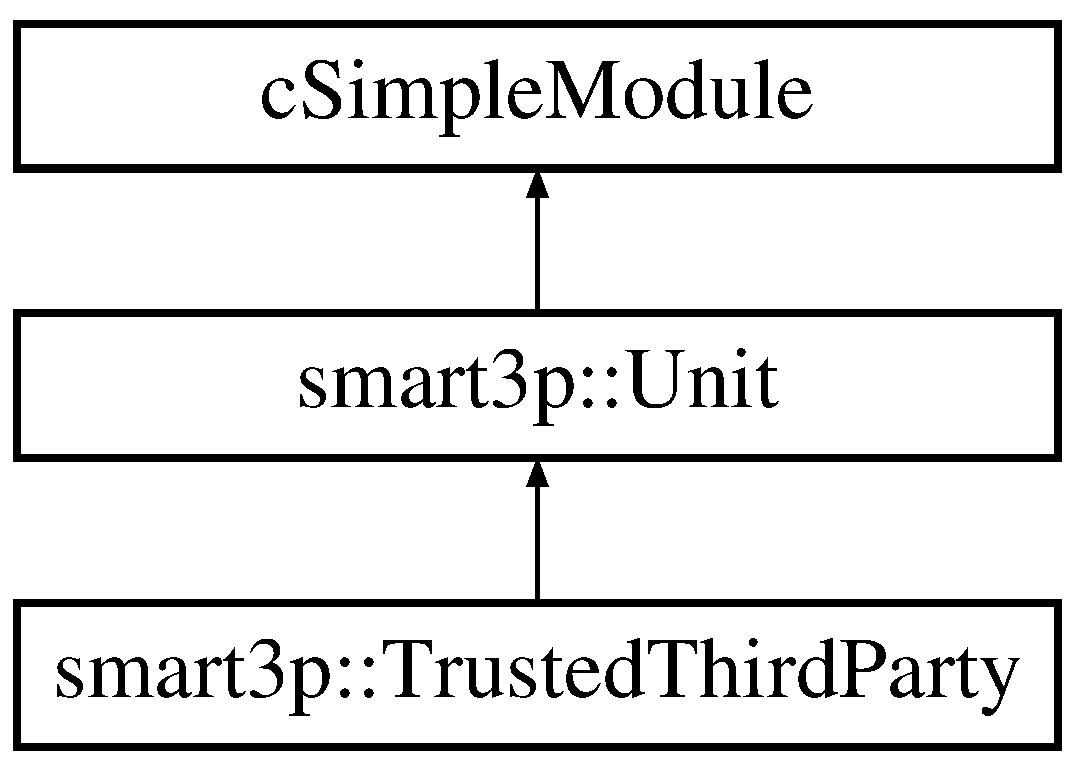
\includegraphics[height=3.000000cm]{classsmart3p_1_1TrustedThirdParty}
\end{center}
\end{figure}
\subsection*{Public Member Functions}
\begin{DoxyCompactItemize}
\item 
void \hyperlink{classsmart3p_1_1TrustedThirdParty_aa6b9b6e4731061d43609acbf02ebbb81}{print} (char $\ast$)
\begin{DoxyCompactList}\small\item\em Print debug messages. \end{DoxyCompactList}\end{DoxyCompactItemize}
\subsection*{Protected Member Functions}
\begin{DoxyCompactItemize}
\item 
virtual void \hyperlink{classsmart3p_1_1TrustedThirdParty_a07be5c50d1ec6307e02c20ee9829d0e4}{initialize} ()
\item 
virtual void \hyperlink{classsmart3p_1_1TrustedThirdParty_adedb95022442b9c7f2bc1de5f4c17a76}{timed\+Handle\+Message} (c\+Message $\ast$msg)
\begin{DoxyCompactList}\small\item\em Default message handler. \end{DoxyCompactList}\end{DoxyCompactItemize}
\subsection*{Additional Inherited Members}


\subsection{Detailed Description}
Trusted Thrid Party for the simulation. 

Definition at line 28 of file Trusted\+Third\+Party.\+h.



\subsection{Member Function Documentation}
\mbox{\Hypertarget{classsmart3p_1_1TrustedThirdParty_a07be5c50d1ec6307e02c20ee9829d0e4}\label{classsmart3p_1_1TrustedThirdParty_a07be5c50d1ec6307e02c20ee9829d0e4}} 
\index{smart3p\+::\+Trusted\+Third\+Party@{smart3p\+::\+Trusted\+Third\+Party}!initialize@{initialize}}
\index{initialize@{initialize}!smart3p\+::\+Trusted\+Third\+Party@{smart3p\+::\+Trusted\+Third\+Party}}
\subsubsection{\texorpdfstring{initialize()}{initialize()}}
{\footnotesize\ttfamily void smart3p\+::\+Trusted\+Third\+Party\+::initialize (\begin{DoxyParamCaption}{ }\end{DoxyParamCaption})\hspace{0.3cm}{\ttfamily [protected]}, {\ttfamily [virtual]}}



Definition at line 29 of file Trusted\+Third\+Party.\+cc.

\mbox{\Hypertarget{classsmart3p_1_1TrustedThirdParty_aa6b9b6e4731061d43609acbf02ebbb81}\label{classsmart3p_1_1TrustedThirdParty_aa6b9b6e4731061d43609acbf02ebbb81}} 
\index{smart3p\+::\+Trusted\+Third\+Party@{smart3p\+::\+Trusted\+Third\+Party}!print@{print}}
\index{print@{print}!smart3p\+::\+Trusted\+Third\+Party@{smart3p\+::\+Trusted\+Third\+Party}}
\subsubsection{\texorpdfstring{print()}{print()}}
{\footnotesize\ttfamily void smart3p\+::\+Trusted\+Third\+Party\+::print (\begin{DoxyParamCaption}\item[{char $\ast$}]{ }\end{DoxyParamCaption})}



Print debug messages. 

\mbox{\Hypertarget{classsmart3p_1_1TrustedThirdParty_adedb95022442b9c7f2bc1de5f4c17a76}\label{classsmart3p_1_1TrustedThirdParty_adedb95022442b9c7f2bc1de5f4c17a76}} 
\index{smart3p\+::\+Trusted\+Third\+Party@{smart3p\+::\+Trusted\+Third\+Party}!timed\+Handle\+Message@{timed\+Handle\+Message}}
\index{timed\+Handle\+Message@{timed\+Handle\+Message}!smart3p\+::\+Trusted\+Third\+Party@{smart3p\+::\+Trusted\+Third\+Party}}
\subsubsection{\texorpdfstring{timed\+Handle\+Message()}{timedHandleMessage()}}
{\footnotesize\ttfamily void smart3p\+::\+Trusted\+Third\+Party\+::timed\+Handle\+Message (\begin{DoxyParamCaption}\item[{c\+Message $\ast$}]{msg }\end{DoxyParamCaption})\hspace{0.3cm}{\ttfamily [protected]}, {\ttfamily [virtual]}}



Default message handler. 



Reimplemented from \hyperlink{classsmart3p_1_1Unit_a93f16f43dec69d23d8588f3b60c96d69}{smart3p\+::\+Unit}.



Definition at line 39 of file Trusted\+Third\+Party.\+cc.



References T\+T\+P\+Adapter\+::finish\+Session\+Key\+Exchange(), T\+T\+P\+Adapter\+::process\+Data\+From\+S\+M(), T\+T\+P\+Adapter\+::register\+At\+U\+C(), T\+T\+P\+Adapter\+::register\+Info\+From\+U\+C(), T\+T\+P\+Adapter\+::register\+S\+M(), and T\+T\+P\+Adapter\+::start\+Session\+Key\+Exchange().



The documentation for this class was generated from the following files\+:\begin{DoxyCompactItemize}
\item 
src/\hyperlink{TrustedThirdParty_8h}{Trusted\+Third\+Party.\+h}\item 
src/\hyperlink{TrustedThirdParty_8cc}{Trusted\+Third\+Party.\+cc}\end{DoxyCompactItemize}

\hypertarget{classTTPAdapter}{}\section{T\+T\+P\+Adapter Class Reference}
\label{classTTPAdapter}\index{T\+T\+P\+Adapter@{T\+T\+P\+Adapter}}


Trusted Thrid Party \hyperlink{classAdapter}{Adapter}.  




{\ttfamily \#include $<$T\+T\+P\+Adapter.\+h$>$}

Inheritance diagram for T\+T\+P\+Adapter\+:\begin{figure}[H]
\begin{center}
\leavevmode
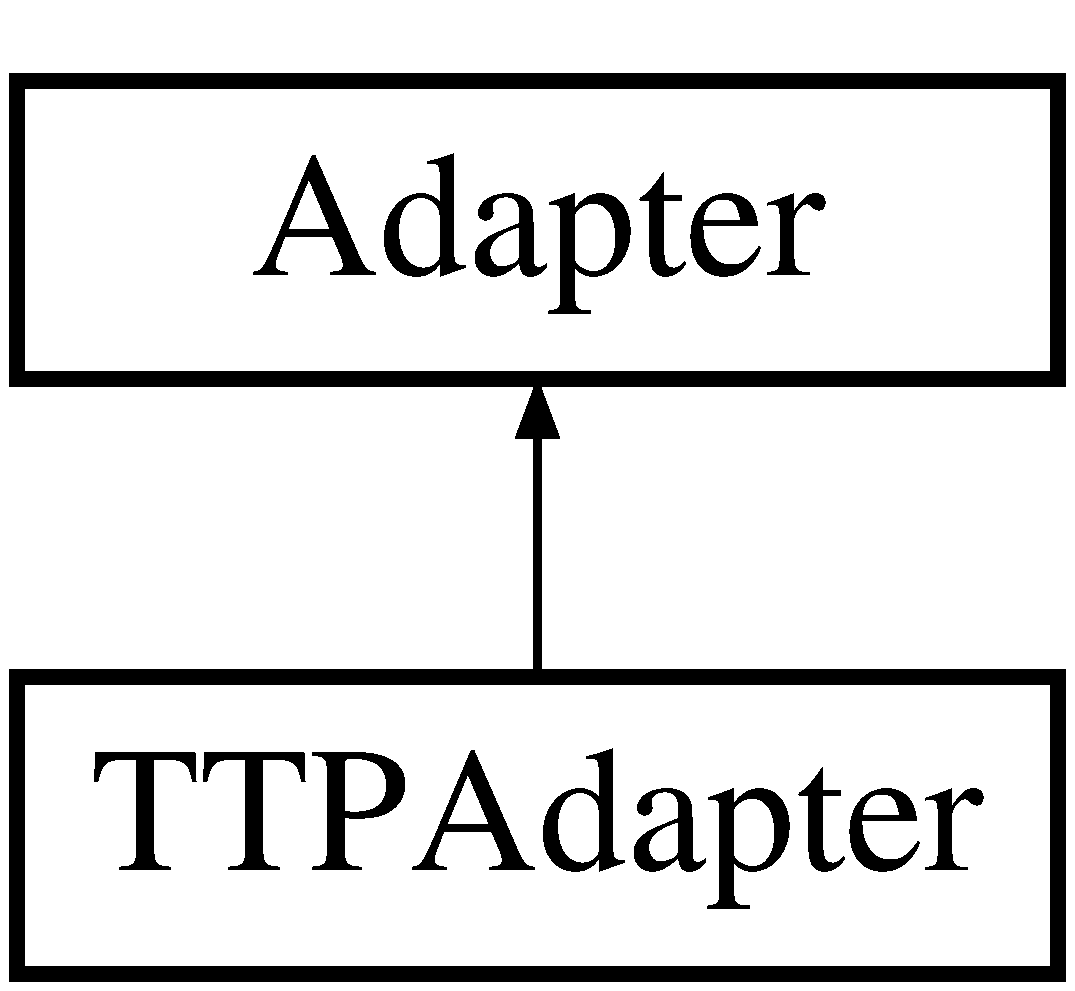
\includegraphics[height=2.000000cm]{classTTPAdapter}
\end{center}
\end{figure}
\subsection*{Public Member Functions}
\begin{DoxyCompactItemize}
\item 
\hyperlink{classTTPAdapter_a47fcddf78f8e0b494fe2f6a79f16c762}{T\+T\+P\+Adapter} (int id)
\item 
\hyperlink{classTTPAdapter_a2c64e6c544cf9aa5e715ecb91bae2baa}{T\+T\+P\+Adapter} (int id, \hyperlink{classsmart3p_1_1Unit}{smart3p\+::\+Unit} $\ast$u)
\item 
\hyperlink{classTTPAdapter_aac9a02ae55c0ba9752869e5c7f1a3d79}{$\sim$\+T\+T\+P\+Adapter} ()
\item 
void \hyperlink{classTTPAdapter_ad53a31939a278d3c114f79bea64f81f0}{register\+SM} (omnetpp\+::c\+Message $\ast$)
\item 
omnetpp\+::c\+Queue $\ast$ \hyperlink{classTTPAdapter_a1e5405c3ac74693b2a542dd72ad44012}{start\+Session\+Key\+Exchange} ()
\item 
omnetpp\+::c\+Message $\ast$ \hyperlink{classTTPAdapter_a3cfb4c68f5a6bf562584f7710b411e4a}{finish\+Session\+Key\+Exchange} (omnetpp\+::c\+Message $\ast$)
\item 
void \hyperlink{classTTPAdapter_a9aa8948a5224e2cf567eaacb2dcee6ab}{register\+Info\+From\+UC} (omnetpp\+::c\+Message $\ast$)
\item 
omnetpp\+::c\+Message $\ast$ \hyperlink{classTTPAdapter_a4eba454018be25436474c37ae1bbe083}{register\+At\+UC} ()
\item 
void \hyperlink{classTTPAdapter_ab69604de63c3f769a10ec33168611274}{process\+Data\+From\+SM} (omnetpp\+::c\+Message $\ast$)
\end{DoxyCompactItemize}
\subsection*{Additional Inherited Members}


\subsection{Detailed Description}
Trusted Thrid Party \hyperlink{classAdapter}{Adapter}. 

Definition at line 11 of file T\+T\+P\+Adapter.\+h.



\subsection{Constructor \& Destructor Documentation}
\mbox{\Hypertarget{classTTPAdapter_a47fcddf78f8e0b494fe2f6a79f16c762}\label{classTTPAdapter_a47fcddf78f8e0b494fe2f6a79f16c762}} 
\index{T\+T\+P\+Adapter@{T\+T\+P\+Adapter}!T\+T\+P\+Adapter@{T\+T\+P\+Adapter}}
\index{T\+T\+P\+Adapter@{T\+T\+P\+Adapter}!T\+T\+P\+Adapter@{T\+T\+P\+Adapter}}
\subsubsection{\texorpdfstring{T\+T\+P\+Adapter()}{TTPAdapter()}\hspace{0.1cm}{\footnotesize\ttfamily [1/2]}}
{\footnotesize\ttfamily T\+T\+P\+Adapter\+::\+T\+T\+P\+Adapter (\begin{DoxyParamCaption}\item[{int}]{id }\end{DoxyParamCaption})}


\begin{DoxyParams}{Parameters}
{\em id} & Trusted Third Party ID \\
\hline
\end{DoxyParams}


Definition at line 11 of file T\+T\+P\+Adapter.\+cc.

\mbox{\Hypertarget{classTTPAdapter_a2c64e6c544cf9aa5e715ecb91bae2baa}\label{classTTPAdapter_a2c64e6c544cf9aa5e715ecb91bae2baa}} 
\index{T\+T\+P\+Adapter@{T\+T\+P\+Adapter}!T\+T\+P\+Adapter@{T\+T\+P\+Adapter}}
\index{T\+T\+P\+Adapter@{T\+T\+P\+Adapter}!T\+T\+P\+Adapter@{T\+T\+P\+Adapter}}
\subsubsection{\texorpdfstring{T\+T\+P\+Adapter()}{TTPAdapter()}\hspace{0.1cm}{\footnotesize\ttfamily [2/2]}}
{\footnotesize\ttfamily T\+T\+P\+Adapter\+::\+T\+T\+P\+Adapter (\begin{DoxyParamCaption}\item[{int}]{id,  }\item[{\hyperlink{classsmart3p_1_1Unit}{smart3p\+::\+Unit} $\ast$}]{u }\end{DoxyParamCaption})}


\begin{DoxyParams}{Parameters}
{\em id} & Trusted Third Party ID \\
\hline
{\em u} & Output unit class (used for debugging) \\
\hline
\end{DoxyParams}


Definition at line 16 of file T\+T\+P\+Adapter.\+cc.

\mbox{\Hypertarget{classTTPAdapter_aac9a02ae55c0ba9752869e5c7f1a3d79}\label{classTTPAdapter_aac9a02ae55c0ba9752869e5c7f1a3d79}} 
\index{T\+T\+P\+Adapter@{T\+T\+P\+Adapter}!````~T\+T\+P\+Adapter@{$\sim$\+T\+T\+P\+Adapter}}
\index{````~T\+T\+P\+Adapter@{$\sim$\+T\+T\+P\+Adapter}!T\+T\+P\+Adapter@{T\+T\+P\+Adapter}}
\subsubsection{\texorpdfstring{$\sim$\+T\+T\+P\+Adapter()}{~TTPAdapter()}}
{\footnotesize\ttfamily T\+T\+P\+Adapter\+::$\sim$\+T\+T\+P\+Adapter (\begin{DoxyParamCaption}{ }\end{DoxyParamCaption})}



Definition at line 21 of file T\+T\+P\+Adapter.\+cc.



\subsection{Member Function Documentation}
\mbox{\Hypertarget{classTTPAdapter_a3cfb4c68f5a6bf562584f7710b411e4a}\label{classTTPAdapter_a3cfb4c68f5a6bf562584f7710b411e4a}} 
\index{T\+T\+P\+Adapter@{T\+T\+P\+Adapter}!finish\+Session\+Key\+Exchange@{finish\+Session\+Key\+Exchange}}
\index{finish\+Session\+Key\+Exchange@{finish\+Session\+Key\+Exchange}!T\+T\+P\+Adapter@{T\+T\+P\+Adapter}}
\subsubsection{\texorpdfstring{finish\+Session\+Key\+Exchange()}{finishSessionKeyExchange()}}
{\footnotesize\ttfamily omnetpp\+::c\+Message $\ast$ T\+T\+P\+Adapter\+::finish\+Session\+Key\+Exchange (\begin{DoxyParamCaption}\item[{omnetpp\+::c\+Message $\ast$}]{msg }\end{DoxyParamCaption})}

Finishes the session key exchange phase, forwarding the final state to the Smart Meter. 

Definition at line 53 of file T\+T\+P\+Adapter.\+cc.



References S\+M\+Imp\+::\+H\+M\+A\+C\+Payload\+::c1, S\+M\+Imp\+::\+H\+M\+A\+C\+Payload\+::c2, S\+M\+Imp\+::\+Trusted\+Party\+::confirm\+Session(), S\+M\+Imp\+::\+Packet\+::dest, S\+M\+Imp\+::\+H\+M\+A\+C\+Payload\+::hmac, S\+M\+Imp\+::\+H\+M\+A\+C\+Payload\+::id, S\+M\+Imp\+::\+Key\+::partial, S\+M\+Imp\+::\+Key\+::piece, S\+M\+Imp\+::\+Packet\+::pl, S\+M\+Imp\+::\+Trusted\+Party\+::recieve\+H\+M\+A\+C(), and S\+M\+Imp\+::\+H\+M\+A\+C\+Payload\+::time\+Stamp.

\mbox{\Hypertarget{classTTPAdapter_ab69604de63c3f769a10ec33168611274}\label{classTTPAdapter_ab69604de63c3f769a10ec33168611274}} 
\index{T\+T\+P\+Adapter@{T\+T\+P\+Adapter}!process\+Data\+From\+SM@{process\+Data\+From\+SM}}
\index{process\+Data\+From\+SM@{process\+Data\+From\+SM}!T\+T\+P\+Adapter@{T\+T\+P\+Adapter}}
\subsubsection{\texorpdfstring{process\+Data\+From\+S\+M()}{processDataFromSM()}}
{\footnotesize\ttfamily void T\+T\+P\+Adapter\+::process\+Data\+From\+SM (\begin{DoxyParamCaption}\item[{omnetpp\+::c\+Message $\ast$}]{msg }\end{DoxyParamCaption})}

Processes energy consumption data from Smart Meter. 

Definition at line 130 of file T\+T\+P\+Adapter.\+cc.



References Adapter\+::out, Adapter\+::print(), S\+M\+Imp\+::\+Trusted\+Party\+::recieve\+Data(), and Adapter\+::verbose.

\mbox{\Hypertarget{classTTPAdapter_a4eba454018be25436474c37ae1bbe083}\label{classTTPAdapter_a4eba454018be25436474c37ae1bbe083}} 
\index{T\+T\+P\+Adapter@{T\+T\+P\+Adapter}!register\+At\+UC@{register\+At\+UC}}
\index{register\+At\+UC@{register\+At\+UC}!T\+T\+P\+Adapter@{T\+T\+P\+Adapter}}
\subsubsection{\texorpdfstring{register\+At\+U\+C()}{registerAtUC()}}
{\footnotesize\ttfamily omnetpp\+::c\+Message $\ast$ T\+T\+P\+Adapter\+::register\+At\+UC (\begin{DoxyParamCaption}{ }\end{DoxyParamCaption})}

Registers Trusted Thrid Party with Utility Company. 

Definition at line 104 of file T\+T\+P\+Adapter.\+cc.



References S\+M\+Imp\+::\+Requester\+::get\+Id(), and smart3p\+::\+S\+M\+Packet\+::set\+Id().

\mbox{\Hypertarget{classTTPAdapter_a9aa8948a5224e2cf567eaacb2dcee6ab}\label{classTTPAdapter_a9aa8948a5224e2cf567eaacb2dcee6ab}} 
\index{T\+T\+P\+Adapter@{T\+T\+P\+Adapter}!register\+Info\+From\+UC@{register\+Info\+From\+UC}}
\index{register\+Info\+From\+UC@{register\+Info\+From\+UC}!T\+T\+P\+Adapter@{T\+T\+P\+Adapter}}
\subsubsection{\texorpdfstring{register\+Info\+From\+U\+C()}{registerInfoFromUC()}}
{\footnotesize\ttfamily void T\+T\+P\+Adapter\+::register\+Info\+From\+UC (\begin{DoxyParamCaption}\item[{omnetpp\+::c\+Message $\ast$}]{msg }\end{DoxyParamCaption})}

Registers info recievd from Utility Company regarding key generation. 

Definition at line 115 of file T\+T\+P\+Adapter.\+cc.



References S\+M\+Imp\+::\+Requester\+::generate\+Keys(), S\+M\+Imp\+::\+Master\+Key\+::p, and S\+M\+Imp\+::\+Payload\+::params.

\mbox{\Hypertarget{classTTPAdapter_ad53a31939a278d3c114f79bea64f81f0}\label{classTTPAdapter_ad53a31939a278d3c114f79bea64f81f0}} 
\index{T\+T\+P\+Adapter@{T\+T\+P\+Adapter}!register\+SM@{register\+SM}}
\index{register\+SM@{register\+SM}!T\+T\+P\+Adapter@{T\+T\+P\+Adapter}}
\subsubsection{\texorpdfstring{register\+S\+M()}{registerSM()}}
{\footnotesize\ttfamily void T\+T\+P\+Adapter\+::register\+SM (\begin{DoxyParamCaption}\item[{omnetpp\+::c\+Message $\ast$}]{msg }\end{DoxyParamCaption})}

Registers Smart Meter with Trusted Thrid Party 

Definition at line 98 of file T\+T\+P\+Adapter.\+cc.



References smart3p\+::\+S\+M\+Packet\+::get\+Id(), and S\+M\+Imp\+::\+Trusted\+Party\+::register\+S\+M().

\mbox{\Hypertarget{classTTPAdapter_a1e5405c3ac74693b2a542dd72ad44012}\label{classTTPAdapter_a1e5405c3ac74693b2a542dd72ad44012}} 
\index{T\+T\+P\+Adapter@{T\+T\+P\+Adapter}!start\+Session\+Key\+Exchange@{start\+Session\+Key\+Exchange}}
\index{start\+Session\+Key\+Exchange@{start\+Session\+Key\+Exchange}!T\+T\+P\+Adapter@{T\+T\+P\+Adapter}}
\subsubsection{\texorpdfstring{start\+Session\+Key\+Exchange()}{startSessionKeyExchange()}}
{\footnotesize\ttfamily omnetpp\+::c\+Queue $\ast$ T\+T\+P\+Adapter\+::start\+Session\+Key\+Exchange (\begin{DoxyParamCaption}{ }\end{DoxyParamCaption})}

Begins the session key exchange phase. \begin{DoxyReturn}{Returns}
Queue of outgoing packets 
\end{DoxyReturn}


Definition at line 26 of file T\+T\+P\+Adapter.\+cc.



References List$<$ T $>$\+::get(), S\+M\+Imp\+::\+Requester\+::get\+Id(), S\+M\+Imp\+::\+Requester\+::get\+Public\+Mu(), S\+M\+Imp\+::\+Requester\+::get\+Public\+Partial(), S\+M\+Imp\+::\+Trusted\+Party\+::get\+S\+M\+Iterator(), Iterator$<$ T $>$\+::has\+Next(), Iterator$<$ T $>$\+::next(), and smart3p\+::\+S\+M\+Packet\+::set\+Id().



The documentation for this class was generated from the following files\+:\begin{DoxyCompactItemize}
\item 
src/\hyperlink{TTPAdapter_8h}{T\+T\+P\+Adapter.\+h}\item 
src/\hyperlink{TTPAdapter_8cc}{T\+T\+P\+Adapter.\+cc}\end{DoxyCompactItemize}

\hypertarget{classUCAdapter}{}\section{U\+C\+Adapter Class Reference}
\label{classUCAdapter}\index{U\+C\+Adapter@{U\+C\+Adapter}}


Utility Company \hyperlink{classAdapter}{Adapter}.  




{\ttfamily \#include $<$U\+C\+Adapter.\+h$>$}

Inheritance diagram for U\+C\+Adapter\+:\begin{figure}[H]
\begin{center}
\leavevmode
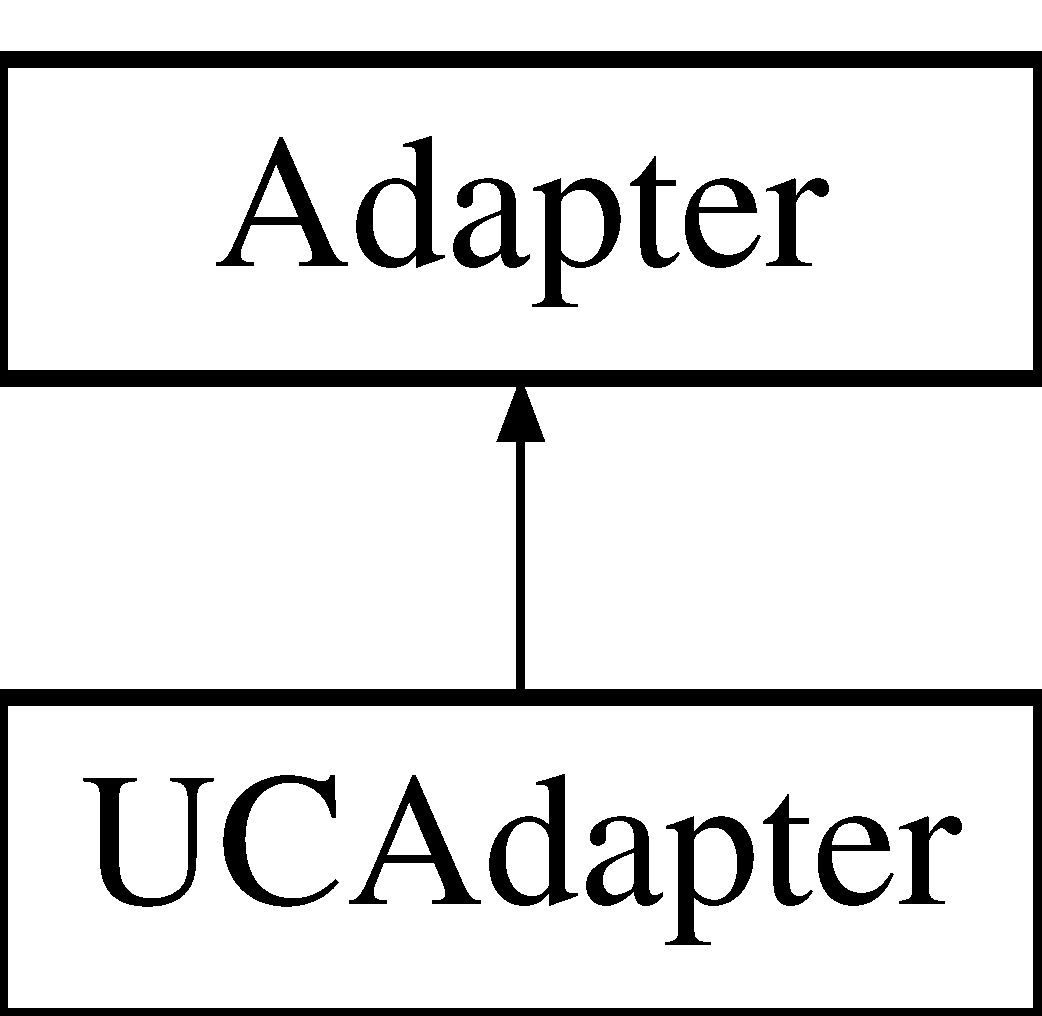
\includegraphics[height=2.000000cm]{classUCAdapter}
\end{center}
\end{figure}
\subsection*{Public Member Functions}
\begin{DoxyCompactItemize}
\item 
\hyperlink{classUCAdapter_ad845819dddba8f4dd674425ff320d99b}{U\+C\+Adapter} (\hyperlink{classsmart3p_1_1Unit}{smart3p\+::\+Unit} $\ast$u)
\item 
\hyperlink{classUCAdapter_a15c10a1542ab5729b6663c342a71e217}{U\+C\+Adapter} ()
\item 
\hyperlink{classUCAdapter_a5d43145233b8a18e92d258aef1d65426}{$\sim$\+U\+C\+Adapter} ()
\item 
omnetpp\+::c\+Message $\ast$ \hyperlink{classUCAdapter_a04ad687c0afed4f04b146742a7bd015f}{register\+SM} (omnetpp\+::c\+Message $\ast$)
\item 
omnetpp\+::c\+Message $\ast$ \hyperlink{classUCAdapter_af76f6694150b1cff5ee307851a501159}{register\+T\+TP} (omnetpp\+::c\+Message $\ast$msg)
\item 
void \hyperlink{classUCAdapter_ab66ce1ddf0945e8d3af7a9e5bf47b411}{finish\+Registering\+T\+TP} (omnetpp\+::c\+Message $\ast$msg)
\item 
omnetpp\+::c\+Message $\ast$ \hyperlink{classUCAdapter_a5d19454ec8881addda7d1f144cae56eb}{session\+Key\+Start\+From\+T\+TP} (omnetpp\+::c\+Message $\ast$msg)
\item 
bool \hyperlink{classUCAdapter_a98ef8576af7f724b687edcf2dc7c3221}{session\+Key\+Exchange\+From\+T\+TP} (omnetpp\+::c\+Message $\ast$msg)
\item 
bool \hyperlink{classUCAdapter_a855d4b0354b46575b99e1c46b746e5ac}{session\+Key\+Exchange\+From\+SM} (omnetpp\+::c\+Message $\ast$msg)
\item 
bool \hyperlink{classUCAdapter_a6554ae131e5cf6c059158061eb629839}{energy\+Consumption\+Processing} (omnetpp\+::c\+Message $\ast$msg)
\end{DoxyCompactItemize}
\subsection*{Additional Inherited Members}


\subsection{Detailed Description}
Utility Company \hyperlink{classAdapter}{Adapter}. 

Definition at line 15 of file U\+C\+Adapter.\+h.



\subsection{Constructor \& Destructor Documentation}
\mbox{\Hypertarget{classUCAdapter_ad845819dddba8f4dd674425ff320d99b}\label{classUCAdapter_ad845819dddba8f4dd674425ff320d99b}} 
\index{U\+C\+Adapter@{U\+C\+Adapter}!U\+C\+Adapter@{U\+C\+Adapter}}
\index{U\+C\+Adapter@{U\+C\+Adapter}!U\+C\+Adapter@{U\+C\+Adapter}}
\subsubsection{\texorpdfstring{U\+C\+Adapter()}{UCAdapter()}\hspace{0.1cm}{\footnotesize\ttfamily [1/2]}}
{\footnotesize\ttfamily U\+C\+Adapter\+::\+U\+C\+Adapter (\begin{DoxyParamCaption}\item[{\hyperlink{classsmart3p_1_1Unit}{smart3p\+::\+Unit} $\ast$}]{u }\end{DoxyParamCaption})}


\begin{DoxyParams}{Parameters}
{\em u} & Output unit class (used for debugging) \\
\hline
\end{DoxyParams}


Definition at line 9 of file U\+C\+Adapter.\+cc.

\mbox{\Hypertarget{classUCAdapter_a15c10a1542ab5729b6663c342a71e217}\label{classUCAdapter_a15c10a1542ab5729b6663c342a71e217}} 
\index{U\+C\+Adapter@{U\+C\+Adapter}!U\+C\+Adapter@{U\+C\+Adapter}}
\index{U\+C\+Adapter@{U\+C\+Adapter}!U\+C\+Adapter@{U\+C\+Adapter}}
\subsubsection{\texorpdfstring{U\+C\+Adapter()}{UCAdapter()}\hspace{0.1cm}{\footnotesize\ttfamily [2/2]}}
{\footnotesize\ttfamily U\+C\+Adapter\+::\+U\+C\+Adapter (\begin{DoxyParamCaption}{ }\end{DoxyParamCaption})}



Definition at line 14 of file U\+C\+Adapter.\+cc.

\mbox{\Hypertarget{classUCAdapter_a5d43145233b8a18e92d258aef1d65426}\label{classUCAdapter_a5d43145233b8a18e92d258aef1d65426}} 
\index{U\+C\+Adapter@{U\+C\+Adapter}!````~U\+C\+Adapter@{$\sim$\+U\+C\+Adapter}}
\index{````~U\+C\+Adapter@{$\sim$\+U\+C\+Adapter}!U\+C\+Adapter@{U\+C\+Adapter}}
\subsubsection{\texorpdfstring{$\sim$\+U\+C\+Adapter()}{~UCAdapter()}}
{\footnotesize\ttfamily U\+C\+Adapter\+::$\sim$\+U\+C\+Adapter (\begin{DoxyParamCaption}{ }\end{DoxyParamCaption})}



Definition at line 19 of file U\+C\+Adapter.\+cc.



\subsection{Member Function Documentation}
\mbox{\Hypertarget{classUCAdapter_a6554ae131e5cf6c059158061eb629839}\label{classUCAdapter_a6554ae131e5cf6c059158061eb629839}} 
\index{U\+C\+Adapter@{U\+C\+Adapter}!energy\+Consumption\+Processing@{energy\+Consumption\+Processing}}
\index{energy\+Consumption\+Processing@{energy\+Consumption\+Processing}!U\+C\+Adapter@{U\+C\+Adapter}}
\subsubsection{\texorpdfstring{energy\+Consumption\+Processing()}{energyConsumptionProcessing()}}
{\footnotesize\ttfamily bool U\+C\+Adapter\+::energy\+Consumption\+Processing (\begin{DoxyParamCaption}\item[{omnetpp\+::c\+Message $\ast$}]{msg }\end{DoxyParamCaption})}

Passes energy consuption data packets to lower-\/level protocol implementation for H\+M\+AC verification. \begin{DoxyReturn}{Returns}
Indicates if verification failed or not (false if failed). 
\end{DoxyReturn}


Definition at line 157 of file U\+C\+Adapter.\+cc.



References session\+Key\+Exchange\+From\+S\+M().

\mbox{\Hypertarget{classUCAdapter_ab66ce1ddf0945e8d3af7a9e5bf47b411}\label{classUCAdapter_ab66ce1ddf0945e8d3af7a9e5bf47b411}} 
\index{U\+C\+Adapter@{U\+C\+Adapter}!finish\+Registering\+T\+TP@{finish\+Registering\+T\+TP}}
\index{finish\+Registering\+T\+TP@{finish\+Registering\+T\+TP}!U\+C\+Adapter@{U\+C\+Adapter}}
\subsubsection{\texorpdfstring{finish\+Registering\+T\+T\+P()}{finishRegisteringTTP()}}
{\footnotesize\ttfamily void U\+C\+Adapter\+::finish\+Registering\+T\+TP (\begin{DoxyParamCaption}\item[{omnetpp\+::c\+Message $\ast$}]{msg }\end{DoxyParamCaption})}

Finalizes Trusted Third Party registration. \mbox{\Hypertarget{classUCAdapter_a04ad687c0afed4f04b146742a7bd015f}\label{classUCAdapter_a04ad687c0afed4f04b146742a7bd015f}} 
\index{U\+C\+Adapter@{U\+C\+Adapter}!register\+SM@{register\+SM}}
\index{register\+SM@{register\+SM}!U\+C\+Adapter@{U\+C\+Adapter}}
\subsubsection{\texorpdfstring{register\+S\+M()}{registerSM()}}
{\footnotesize\ttfamily omnetpp\+::c\+Message $\ast$ U\+C\+Adapter\+::register\+SM (\begin{DoxyParamCaption}\item[{omnetpp\+::c\+Message $\ast$}]{msg }\end{DoxyParamCaption})}

Registers Smart Meter with Utility Company. 

Definition at line 24 of file U\+C\+Adapter.\+cc.



References S\+M\+Imp\+::\+Utility\+Company\+::add\+S\+M\+Data(), S\+M\+Imp\+::\+Utility\+Company\+::generate\+Partial\+Keys(), List$<$ T $>$\+::get(), smart3p\+::\+S\+M\+Packet\+::get\+Id(), S\+M\+Imp\+::\+Utility\+Company\+::get\+S\+M(), smart3p\+::\+S\+M\+Packet\+::get\+Sm\+Gate\+I\+D(), S\+M\+Imp\+::\+Utility\+Company\+::register\+S\+M(), and smart3p\+::\+S\+M\+Packet\+::set\+Sm\+Gate\+I\+D().

\mbox{\Hypertarget{classUCAdapter_af76f6694150b1cff5ee307851a501159}\label{classUCAdapter_af76f6694150b1cff5ee307851a501159}} 
\index{U\+C\+Adapter@{U\+C\+Adapter}!register\+T\+TP@{register\+T\+TP}}
\index{register\+T\+TP@{register\+T\+TP}!U\+C\+Adapter@{U\+C\+Adapter}}
\subsubsection{\texorpdfstring{register\+T\+T\+P()}{registerTTP()}}
{\footnotesize\ttfamily omnetpp\+::c\+Message $\ast$ U\+C\+Adapter\+::register\+T\+TP (\begin{DoxyParamCaption}\item[{omnetpp\+::c\+Message $\ast$}]{msg }\end{DoxyParamCaption})}

Registers Trusted Third Party with Utility Company. 

Definition at line 62 of file U\+C\+Adapter.\+cc.



References S\+M\+Imp\+::\+Master\+Key\+::g, S\+M\+Imp\+::\+Utility\+Company\+::generate\+Partial\+Keys(), smart3p\+::\+S\+M\+Packet\+::get\+Id(), S\+M\+Imp\+::\+Master\+Key\+::p, S\+M\+Imp\+::\+Payload\+::params, S\+M\+Imp\+::\+Payload\+::priv, S\+M\+Imp\+::\+Payload\+::pub, S\+M\+Imp\+::\+Master\+Key\+::q, S\+M\+Imp\+::\+Utility\+Company\+::register\+T\+T\+P(), and S\+M\+Imp\+::\+Master\+Key\+::x.

\mbox{\Hypertarget{classUCAdapter_a855d4b0354b46575b99e1c46b746e5ac}\label{classUCAdapter_a855d4b0354b46575b99e1c46b746e5ac}} 
\index{U\+C\+Adapter@{U\+C\+Adapter}!session\+Key\+Exchange\+From\+SM@{session\+Key\+Exchange\+From\+SM}}
\index{session\+Key\+Exchange\+From\+SM@{session\+Key\+Exchange\+From\+SM}!U\+C\+Adapter@{U\+C\+Adapter}}
\subsubsection{\texorpdfstring{session\+Key\+Exchange\+From\+S\+M()}{sessionKeyExchangeFromSM()}}
{\footnotesize\ttfamily bool U\+C\+Adapter\+::session\+Key\+Exchange\+From\+SM (\begin{DoxyParamCaption}\item[{omnetpp\+::c\+Message $\ast$}]{msg }\end{DoxyParamCaption})}

Passes session key exchange data from Smart Meter to lower-\/level protocol implementation. 

Definition at line 133 of file U\+C\+Adapter.\+cc.



References List$<$ T $>$\+::get(), S\+M\+Imp\+::\+Utility\+Company\+::get\+S\+M(), S\+M\+Imp\+::\+H\+M\+A\+C\+Payload\+::id, and S\+M\+Imp\+::\+Utility\+Company\+::verify\+H\+M\+A\+C().

\mbox{\Hypertarget{classUCAdapter_a98ef8576af7f724b687edcf2dc7c3221}\label{classUCAdapter_a98ef8576af7f724b687edcf2dc7c3221}} 
\index{U\+C\+Adapter@{U\+C\+Adapter}!session\+Key\+Exchange\+From\+T\+TP@{session\+Key\+Exchange\+From\+T\+TP}}
\index{session\+Key\+Exchange\+From\+T\+TP@{session\+Key\+Exchange\+From\+T\+TP}!U\+C\+Adapter@{U\+C\+Adapter}}
\subsubsection{\texorpdfstring{session\+Key\+Exchange\+From\+T\+T\+P()}{sessionKeyExchangeFromTTP()}}
{\footnotesize\ttfamily bool U\+C\+Adapter\+::session\+Key\+Exchange\+From\+T\+TP (\begin{DoxyParamCaption}\item[{omnetpp\+::c\+Message $\ast$}]{msg }\end{DoxyParamCaption})}

Passes session key exchange data from Trusted Thrid Party to lower-\/level protocol implementation. 

Definition at line 107 of file U\+C\+Adapter.\+cc.



References List$<$ T $>$\+::get(), S\+M\+Imp\+::\+Utility\+Company\+::get\+S\+Mby\+Anon\+Id(), S\+M\+Imp\+::\+H\+M\+A\+C\+Payload\+::id, smart3p\+::\+S\+M\+Packet\+::set\+Coll\+Gate\+I\+D(), smart3p\+::\+S\+M\+Packet\+::set\+Sm\+Gate\+I\+D(), and S\+M\+Imp\+::\+Utility\+Company\+::verify\+H\+M\+A\+C().

\mbox{\Hypertarget{classUCAdapter_a5d19454ec8881addda7d1f144cae56eb}\label{classUCAdapter_a5d19454ec8881addda7d1f144cae56eb}} 
\index{U\+C\+Adapter@{U\+C\+Adapter}!session\+Key\+Start\+From\+T\+TP@{session\+Key\+Start\+From\+T\+TP}}
\index{session\+Key\+Start\+From\+T\+TP@{session\+Key\+Start\+From\+T\+TP}!U\+C\+Adapter@{U\+C\+Adapter}}
\subsubsection{\texorpdfstring{session\+Key\+Start\+From\+T\+T\+P()}{sessionKeyStartFromTTP()}}
{\footnotesize\ttfamily omnetpp\+::c\+Message $\ast$ U\+C\+Adapter\+::session\+Key\+Start\+From\+T\+TP (\begin{DoxyParamCaption}\item[{omnetpp\+::c\+Message $\ast$}]{msg }\end{DoxyParamCaption})}

Passes session key start signal to the lower-\/level protocol implementation. 

Definition at line 91 of file U\+C\+Adapter.\+cc.



References List$<$ T $>$\+::get(), S\+M\+Imp\+::\+Utility\+Company\+::get\+S\+Mby\+Anon\+Id(), smart3p\+::\+S\+M\+Packet\+::set\+Coll\+Gate\+I\+D(), and smart3p\+::\+S\+M\+Packet\+::set\+Sm\+Gate\+I\+D().



The documentation for this class was generated from the following files\+:\begin{DoxyCompactItemize}
\item 
src/\hyperlink{UCAdapter_8h}{U\+C\+Adapter.\+h}\item 
src/\hyperlink{UCAdapter_8cc}{U\+C\+Adapter.\+cc}\end{DoxyCompactItemize}

\hypertarget{classsmart3p_1_1Unit}{}\section{smart3p\+:\+:Unit Class Reference}
\label{classsmart3p_1_1Unit}\index{smart3p\+::\+Unit@{smart3p\+::\+Unit}}


Abstract class for the simulation.  




{\ttfamily \#include $<$Unit.\+h$>$}

Inheritance diagram for smart3p\+:\+:Unit\+:\begin{figure}[H]
\begin{center}
\leavevmode
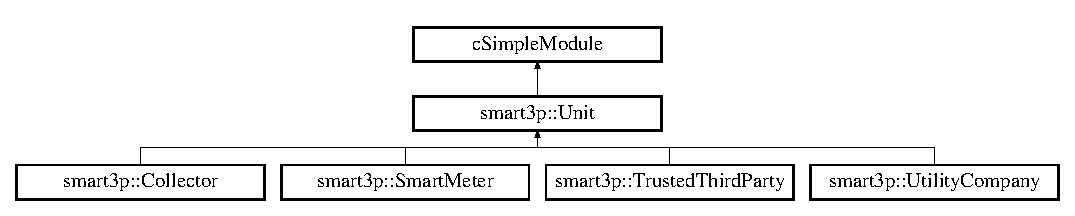
\includegraphics[height=2.456140cm]{classsmart3p_1_1Unit}
\end{center}
\end{figure}
\subsection*{Public Member Functions}
\begin{DoxyCompactItemize}
\item 
\hyperlink{classsmart3p_1_1Unit_ac650bc01f4016ce66b056a9a37793697}{Unit} ()
\begin{DoxyCompactList}\small\item\em Default constrcutor. \end{DoxyCompactList}\item 
virtual \hyperlink{classsmart3p_1_1Unit_af5ab11eebd455ae312399fa3ba813e1b}{$\sim$\+Unit} ()
\item 
void \hyperlink{classsmart3p_1_1Unit_a832d0c6a67960a6d7911df721eda7527}{print} (char $\ast$s)
\end{DoxyCompactItemize}
\subsection*{Protected Member Functions}
\begin{DoxyCompactItemize}
\item 
virtual void \hyperlink{classsmart3p_1_1Unit_a93f16f43dec69d23d8588f3b60c96d69}{timed\+Handle\+Message} (c\+Message $\ast$msg)
\item 
void \hyperlink{classsmart3p_1_1Unit_a7763e2e6ec9e31c7a4743bf674351c13}{handle\+Message} (c\+Message $\ast$msg)
\begin{DoxyCompactList}\small\item\em Main message handler. \end{DoxyCompactList}\end{DoxyCompactItemize}
\subsection*{Protected Attributes}
\begin{DoxyCompactItemize}
\item 
c\+Message $\ast$ \hyperlink{classsmart3p_1_1Unit_a48c180587dfed5ccd985f52f4fab6001}{timeout\+Event}
\item 
double \hyperlink{classsmart3p_1_1Unit_a227ec26ef4734fb25d0e697ff3952e8a}{wait\+For\+Delivery}
\end{DoxyCompactItemize}


\subsection{Detailed Description}
Abstract class for the simulation. 

An abstract class designed to be extended by the nodes within the simulation. 

Definition at line 29 of file Unit.\+h.



\subsection{Constructor \& Destructor Documentation}
\mbox{\Hypertarget{classsmart3p_1_1Unit_ac650bc01f4016ce66b056a9a37793697}\label{classsmart3p_1_1Unit_ac650bc01f4016ce66b056a9a37793697}} 
\index{smart3p\+::\+Unit@{smart3p\+::\+Unit}!Unit@{Unit}}
\index{Unit@{Unit}!smart3p\+::\+Unit@{smart3p\+::\+Unit}}
\subsubsection{\texorpdfstring{Unit()}{Unit()}}
{\footnotesize\ttfamily smart3p\+::\+Unit\+::\+Unit (\begin{DoxyParamCaption}{ }\end{DoxyParamCaption})}



Default constrcutor. 



Definition at line 20 of file Unit.\+cc.



References timeout\+Event, and wait\+For\+Delivery.

\mbox{\Hypertarget{classsmart3p_1_1Unit_af5ab11eebd455ae312399fa3ba813e1b}\label{classsmart3p_1_1Unit_af5ab11eebd455ae312399fa3ba813e1b}} 
\index{smart3p\+::\+Unit@{smart3p\+::\+Unit}!````~Unit@{$\sim$\+Unit}}
\index{````~Unit@{$\sim$\+Unit}!smart3p\+::\+Unit@{smart3p\+::\+Unit}}
\subsubsection{\texorpdfstring{$\sim$\+Unit()}{~Unit()}}
{\footnotesize\ttfamily smart3p\+::\+Unit\+::$\sim$\+Unit (\begin{DoxyParamCaption}{ }\end{DoxyParamCaption})\hspace{0.3cm}{\ttfamily [virtual]}}



Definition at line 27 of file Unit.\+cc.



References timeout\+Event.



\subsection{Member Function Documentation}
\mbox{\Hypertarget{classsmart3p_1_1Unit_a7763e2e6ec9e31c7a4743bf674351c13}\label{classsmart3p_1_1Unit_a7763e2e6ec9e31c7a4743bf674351c13}} 
\index{smart3p\+::\+Unit@{smart3p\+::\+Unit}!handle\+Message@{handle\+Message}}
\index{handle\+Message@{handle\+Message}!smart3p\+::\+Unit@{smart3p\+::\+Unit}}
\subsubsection{\texorpdfstring{handle\+Message()}{handleMessage()}}
{\footnotesize\ttfamily void smart3p\+::\+Unit\+::handle\+Message (\begin{DoxyParamCaption}\item[{c\+Message $\ast$}]{msg }\end{DoxyParamCaption})\hspace{0.3cm}{\ttfamily [protected]}}



Main message handler. 

Main message handler. 
\begin{DoxyParams}{Parameters}
{\em msg} & Input message to be handled. \\
\hline
\end{DoxyParams}
\begin{DoxySeeAlso}{See also}
smart3\+P\+::\+Smart\+Meter\+::handle\+Message(c\+Message $\ast$msg), smart3\+P\+::\+Utility\+Company\+::handle\+Message(c\+Message $\ast$msg), smart3\+P\+::\+Trusted\+Third\+Party\+::handle\+Message(c\+Message $\ast$msg) and smart3\+P\+::\+Collector\+::handle\+Message(c\+Message $\ast$msg) 
\end{DoxySeeAlso}


Definition at line 39 of file Unit.\+cc.



References timed\+Handle\+Message().

\mbox{\Hypertarget{classsmart3p_1_1Unit_a832d0c6a67960a6d7911df721eda7527}\label{classsmart3p_1_1Unit_a832d0c6a67960a6d7911df721eda7527}} 
\index{smart3p\+::\+Unit@{smart3p\+::\+Unit}!print@{print}}
\index{print@{print}!smart3p\+::\+Unit@{smart3p\+::\+Unit}}
\subsubsection{\texorpdfstring{print()}{print()}}
{\footnotesize\ttfamily void smart3p\+::\+Unit\+::print (\begin{DoxyParamCaption}\item[{char $\ast$}]{s }\end{DoxyParamCaption})}

Used by \hyperlink{classAdapter}{Adapter} classes to print messages to the simulation screen. 
\begin{DoxyParams}{Parameters}
{\em s} & String to print. \\
\hline
\end{DoxyParams}
\begin{DoxySeeAlso}{See also}
\hyperlink{classAdapter_af928c4508bc6a76e8f9b918d38ffd221}{Adapter\+::print(char$\ast$)} 
\end{DoxySeeAlso}


Definition at line 34 of file Unit.\+cc.

\mbox{\Hypertarget{classsmart3p_1_1Unit_a93f16f43dec69d23d8588f3b60c96d69}\label{classsmart3p_1_1Unit_a93f16f43dec69d23d8588f3b60c96d69}} 
\index{smart3p\+::\+Unit@{smart3p\+::\+Unit}!timed\+Handle\+Message@{timed\+Handle\+Message}}
\index{timed\+Handle\+Message@{timed\+Handle\+Message}!smart3p\+::\+Unit@{smart3p\+::\+Unit}}
\subsubsection{\texorpdfstring{timed\+Handle\+Message()}{timedHandleMessage()}}
{\footnotesize\ttfamily void smart3p\+::\+Unit\+::timed\+Handle\+Message (\begin{DoxyParamCaption}\item[{c\+Message $\ast$}]{msg }\end{DoxyParamCaption})\hspace{0.3cm}{\ttfamily [protected]}, {\ttfamily [virtual]}}

Unused, simply prints te message name. 
\begin{DoxyParams}{Parameters}
{\em msg} & Input message to be handled. \\
\hline
\end{DoxyParams}


Reimplemented in \hyperlink{classsmart3p_1_1UtilityCompany_af5ce80d9f1d293c9be21fa65668c0e74}{smart3p\+::\+Utility\+Company}, \hyperlink{classsmart3p_1_1SmartMeter_a3491294618643d423e8fd3578eb3a439}{smart3p\+::\+Smart\+Meter}, \hyperlink{classsmart3p_1_1TrustedThirdParty_adedb95022442b9c7f2bc1de5f4c17a76}{smart3p\+::\+Trusted\+Third\+Party}, and \hyperlink{classsmart3p_1_1Collector_a1b82f1a10a2579c3ed25bc899220b906}{smart3p\+::\+Collector}.



Definition at line 50 of file Unit.\+cc.



\subsection{Field Documentation}
\mbox{\Hypertarget{classsmart3p_1_1Unit_a48c180587dfed5ccd985f52f4fab6001}\label{classsmart3p_1_1Unit_a48c180587dfed5ccd985f52f4fab6001}} 
\index{smart3p\+::\+Unit@{smart3p\+::\+Unit}!timeout\+Event@{timeout\+Event}}
\index{timeout\+Event@{timeout\+Event}!smart3p\+::\+Unit@{smart3p\+::\+Unit}}
\subsubsection{\texorpdfstring{timeout\+Event}{timeoutEvent}}
{\footnotesize\ttfamily c\+Message$\ast$ smart3p\+::\+Unit\+::timeout\+Event\hspace{0.3cm}{\ttfamily [protected]}}

c\+Message used to signal a timeout event. \begin{DoxySeeAlso}{See also}
\hyperlink{classsmart3p_1_1Unit_a227ec26ef4734fb25d0e697ff3952e8a}{wait\+For\+Delivery} 
\end{DoxySeeAlso}


Definition at line 48 of file Unit.\+h.

\mbox{\Hypertarget{classsmart3p_1_1Unit_a227ec26ef4734fb25d0e697ff3952e8a}\label{classsmart3p_1_1Unit_a227ec26ef4734fb25d0e697ff3952e8a}} 
\index{smart3p\+::\+Unit@{smart3p\+::\+Unit}!wait\+For\+Delivery@{wait\+For\+Delivery}}
\index{wait\+For\+Delivery@{wait\+For\+Delivery}!smart3p\+::\+Unit@{smart3p\+::\+Unit}}
\subsubsection{\texorpdfstring{wait\+For\+Delivery}{waitForDelivery}}
{\footnotesize\ttfamily double smart3p\+::\+Unit\+::wait\+For\+Delivery\hspace{0.3cm}{\ttfamily [protected]}}

Amount of time to wait for the delivery of an outgoing message. \begin{DoxySeeAlso}{See also}
\hyperlink{classsmart3p_1_1Unit_a48c180587dfed5ccd985f52f4fab6001}{timeout\+Event} 
\end{DoxySeeAlso}


Definition at line 53 of file Unit.\+h.



The documentation for this class was generated from the following files\+:\begin{DoxyCompactItemize}
\item 
src/\hyperlink{Unit_8h}{Unit.\+h}\item 
src/\hyperlink{Unit_8cc}{Unit.\+cc}\end{DoxyCompactItemize}

\hypertarget{classsmart3p_1_1UtilityCompany}{}\section{smart3p\+:\+:Utility\+Company Class Reference}
\label{classsmart3p_1_1UtilityCompany}\index{smart3p\+::\+Utility\+Company@{smart3p\+::\+Utility\+Company}}


Utility Company class for the simulation.  




{\ttfamily \#include $<$Utility\+Company.\+h$>$}

Inheritance diagram for smart3p\+:\+:Utility\+Company\+:\begin{figure}[H]
\begin{center}
\leavevmode
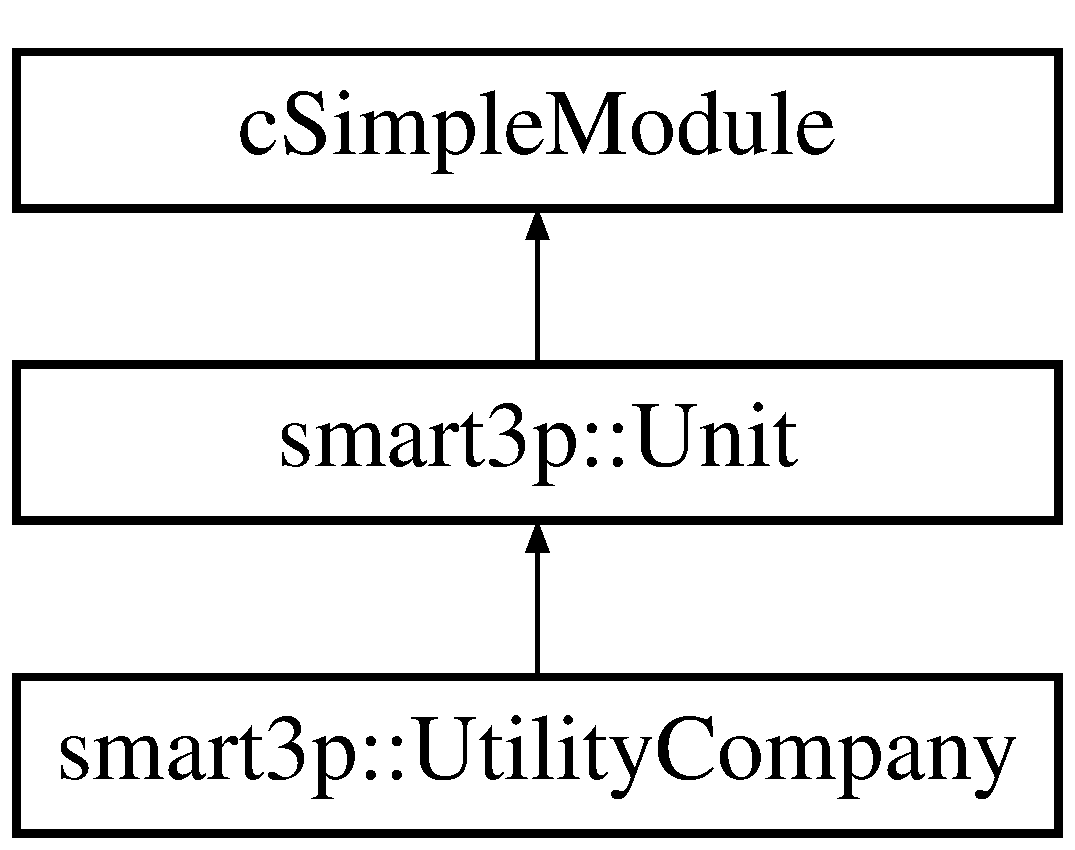
\includegraphics[height=3.000000cm]{classsmart3p_1_1UtilityCompany}
\end{center}
\end{figure}
\subsection*{Public Member Functions}
\begin{DoxyCompactItemize}
\item 
\hyperlink{classsmart3p_1_1UtilityCompany_a2f1eef975aa1798f09da1c1fa79abbe9}{Utility\+Company} ()
\item 
\hyperlink{classsmart3p_1_1UtilityCompany_a6f820a1b7abefa4b2a3cfbe694c7bfc6}{$\sim$\+Utility\+Company} ()
\end{DoxyCompactItemize}
\subsection*{Protected Member Functions}
\begin{DoxyCompactItemize}
\item 
virtual void \hyperlink{classsmart3p_1_1UtilityCompany_a3f7eb4fc092b71349f3ed616e35fba3e}{initialize} ()
\item 
virtual void \hyperlink{classsmart3p_1_1UtilityCompany_af5ce80d9f1d293c9be21fa65668c0e74}{timed\+Handle\+Message} (c\+Message $\ast$msg)
\begin{DoxyCompactList}\small\item\em Default message handler. \end{DoxyCompactList}\end{DoxyCompactItemize}
\subsection*{Additional Inherited Members}


\subsection{Detailed Description}
Utility Company class for the simulation. 

Definition at line 31 of file Utility\+Company.\+h.



\subsection{Constructor \& Destructor Documentation}
\mbox{\Hypertarget{classsmart3p_1_1UtilityCompany_a2f1eef975aa1798f09da1c1fa79abbe9}\label{classsmart3p_1_1UtilityCompany_a2f1eef975aa1798f09da1c1fa79abbe9}} 
\index{smart3p\+::\+Utility\+Company@{smart3p\+::\+Utility\+Company}!Utility\+Company@{Utility\+Company}}
\index{Utility\+Company@{Utility\+Company}!smart3p\+::\+Utility\+Company@{smart3p\+::\+Utility\+Company}}
\subsubsection{\texorpdfstring{Utility\+Company()}{UtilityCompany()}}
{\footnotesize\ttfamily smart3p\+::\+Utility\+Company\+::\+Utility\+Company (\begin{DoxyParamCaption}{ }\end{DoxyParamCaption})}



Definition at line 14 of file Utility\+Company.\+cc.

\mbox{\Hypertarget{classsmart3p_1_1UtilityCompany_a6f820a1b7abefa4b2a3cfbe694c7bfc6}\label{classsmart3p_1_1UtilityCompany_a6f820a1b7abefa4b2a3cfbe694c7bfc6}} 
\index{smart3p\+::\+Utility\+Company@{smart3p\+::\+Utility\+Company}!````~Utility\+Company@{$\sim$\+Utility\+Company}}
\index{````~Utility\+Company@{$\sim$\+Utility\+Company}!smart3p\+::\+Utility\+Company@{smart3p\+::\+Utility\+Company}}
\subsubsection{\texorpdfstring{$\sim$\+Utility\+Company()}{~UtilityCompany()}}
{\footnotesize\ttfamily smart3p\+::\+Utility\+Company\+::$\sim$\+Utility\+Company (\begin{DoxyParamCaption}{ }\end{DoxyParamCaption})}



Definition at line 21 of file Utility\+Company.\+cc.



\subsection{Member Function Documentation}
\mbox{\Hypertarget{classsmart3p_1_1UtilityCompany_a3f7eb4fc092b71349f3ed616e35fba3e}\label{classsmart3p_1_1UtilityCompany_a3f7eb4fc092b71349f3ed616e35fba3e}} 
\index{smart3p\+::\+Utility\+Company@{smart3p\+::\+Utility\+Company}!initialize@{initialize}}
\index{initialize@{initialize}!smart3p\+::\+Utility\+Company@{smart3p\+::\+Utility\+Company}}
\subsubsection{\texorpdfstring{initialize()}{initialize()}}
{\footnotesize\ttfamily void smart3p\+::\+Utility\+Company\+::initialize (\begin{DoxyParamCaption}{ }\end{DoxyParamCaption})\hspace{0.3cm}{\ttfamily [protected]}, {\ttfamily [virtual]}}



Definition at line 26 of file Utility\+Company.\+cc.



References smart3p\+::\+Meter\+Data\+::anonym\+ID, smart3p\+::\+Meter\+Data\+::coll\+Gate, smart3p\+::\+S\+M\+Packet\+::get\+Coll\+Gate\+I\+D(), smart3p\+::\+S\+M\+Packet\+::get\+Extra\+Info(), smart3p\+::\+S\+M\+Packet\+::get\+Id(), smart3p\+::\+S\+M\+Packet\+::get\+Sm\+Gate\+I\+D(), smart3p\+::\+Meter\+Data\+::secret\+S\+Mto\+U\+Ckey, and smart3p\+::\+Meter\+Data\+::sm\+Gate.

\mbox{\Hypertarget{classsmart3p_1_1UtilityCompany_af5ce80d9f1d293c9be21fa65668c0e74}\label{classsmart3p_1_1UtilityCompany_af5ce80d9f1d293c9be21fa65668c0e74}} 
\index{smart3p\+::\+Utility\+Company@{smart3p\+::\+Utility\+Company}!timed\+Handle\+Message@{timed\+Handle\+Message}}
\index{timed\+Handle\+Message@{timed\+Handle\+Message}!smart3p\+::\+Utility\+Company@{smart3p\+::\+Utility\+Company}}
\subsubsection{\texorpdfstring{timed\+Handle\+Message()}{timedHandleMessage()}}
{\footnotesize\ttfamily void smart3p\+::\+Utility\+Company\+::timed\+Handle\+Message (\begin{DoxyParamCaption}\item[{c\+Message $\ast$}]{msg }\end{DoxyParamCaption})\hspace{0.3cm}{\ttfamily [protected]}, {\ttfamily [virtual]}}



Default message handler. 



Reimplemented from \hyperlink{classsmart3p_1_1Unit_a93f16f43dec69d23d8588f3b60c96d69}{smart3p\+::\+Unit}.



Definition at line 45 of file Utility\+Company.\+cc.



References U\+C\+Adapter\+::energy\+Consumption\+Processing(), smart3p\+::\+S\+M\+Packet\+::get\+Coll\+Gate\+I\+D(), smart3p\+::\+S\+M\+Packet\+::get\+Id(), smart3p\+::\+S\+M\+Packet\+::get\+Sm\+Gate\+I\+D(), U\+C\+Adapter\+::register\+S\+M(), U\+C\+Adapter\+::register\+T\+T\+P(), U\+C\+Adapter\+::session\+Key\+Exchange\+From\+S\+M(), U\+C\+Adapter\+::session\+Key\+Exchange\+From\+T\+T\+P(), U\+C\+Adapter\+::session\+Key\+Start\+From\+T\+T\+P(), smart3p\+::\+S\+M\+Packet\+::set\+Coll\+Gate\+I\+D(), smart3p\+::\+S\+M\+Packet\+::set\+Id(), and smart3p\+::\+S\+M\+Packet\+::set\+Sm\+Gate\+I\+D().



The documentation for this class was generated from the following files\+:\begin{DoxyCompactItemize}
\item 
src/\hyperlink{UtilityCompany_8h}{Utility\+Company.\+h}\item 
src/\hyperlink{UtilityCompany_8cc}{Utility\+Company.\+cc}\end{DoxyCompactItemize}

\hypertarget{classSMImp_1_1UtilityCompany}{}\section{S\+M\+Imp\+:\+:Utility\+Company Class Reference}
\label{classSMImp_1_1UtilityCompany}\index{S\+M\+Imp\+::\+Utility\+Company@{S\+M\+Imp\+::\+Utility\+Company}}


Utility Company protocol-\/level implementation.  




{\ttfamily \#include $<$Utility\+Company.\+h$>$}

\subsection*{Public Member Functions}
\begin{DoxyCompactItemize}
\item 
\hyperlink{classSMImp_1_1UtilityCompany_a39c0aca6d615398d97d475b52ee22e89}{Utility\+Company} (S\+H\+A1 $\ast$)
\item 
\hyperlink{classSMImp_1_1UtilityCompany_ab0f04eabfbaf56660c1d199da8170fe0}{Utility\+Company} ()
\item 
\hyperlink{classSMImp_1_1UtilityCompany_a9ef6bb1e7d8032eb305cb227cd68251d}{$\sim$\+Utility\+Company} ()
\item 
bool \hyperlink{classSMImp_1_1UtilityCompany_adeb454bff89a79e454d433bc1ccd448e}{generate\+Key} (Integer q, const Integer \&max, const Integer \&equiv, const Integer \&mod)
\item 
\hyperlink{structSMImp_1_1Payload}{Payload} \hyperlink{classSMImp_1_1UtilityCompany_accfd3e076199f63e5c52ac909976b46a}{generate\+Partial\+Keys} (Integer id)
\item 
bool \hyperlink{classSMImp_1_1UtilityCompany_a5acda2036141ad86d910132004e73b5a}{verify\+H\+M\+AC} (Integer id, \hyperlink{structSMImp_1_1HMACPayload}{H\+M\+A\+C\+Payload} payload)
\item 
void \hyperlink{classSMImp_1_1UtilityCompany_a08a727386b9f32478395975b062d221f}{register\+SM} (Integer $\ast$id)
\item 
void \hyperlink{classSMImp_1_1UtilityCompany_af4559cc4400f5448719aceb32cc53656}{register\+T\+TP} (Integer $\ast$id)
\item 
\hyperlink{classList}{List}$<$ Integer $>$ $\ast$ \hyperlink{classSMImp_1_1UtilityCompany_a76d86a7b253eeb6652dc537d756cbdaf}{get\+S\+Mby\+Anon\+Id} (Integer id)
\item 
\hyperlink{classList}{List}$<$ Integer $>$ $\ast$ \hyperlink{classSMImp_1_1UtilityCompany_a24c3df26cca4ca6ea6855464f2db5249}{get\+SM} (Integer id)
\item 
\hyperlink{classList}{List}$<$ Integer $>$ $\ast$ \hyperlink{classSMImp_1_1UtilityCompany_a3e0d30043e9d880b8f8447232af914c2}{get\+T\+TP} (Integer id)
\item 
void \hyperlink{classSMImp_1_1UtilityCompany_a9e6da1e8015a803748b644d186619a8f}{add\+S\+M\+Data} (Integer $\ast$id, Integer $\ast$data)
\item 
void \hyperlink{classSMImp_1_1UtilityCompany_a03e5d17d5403d9f7527b81d82156650c}{add\+T\+T\+P\+Data} (Integer $\ast$id, Integer $\ast$data)
\item 
int \hyperlink{classSMImp_1_1UtilityCompany_a62d792edc023bd9b8bad3cfdc76f985b}{get\+T\+T\+P\+Size} (Integer $\ast$id)
\end{DoxyCompactItemize}


\subsection{Detailed Description}
Utility Company protocol-\/level implementation. 

Definition at line 12 of file Utility\+Company.\+h.



\subsection{Constructor \& Destructor Documentation}
\mbox{\Hypertarget{classSMImp_1_1UtilityCompany_a39c0aca6d615398d97d475b52ee22e89}\label{classSMImp_1_1UtilityCompany_a39c0aca6d615398d97d475b52ee22e89}} 
\index{S\+M\+Imp\+::\+Utility\+Company@{S\+M\+Imp\+::\+Utility\+Company}!Utility\+Company@{Utility\+Company}}
\index{Utility\+Company@{Utility\+Company}!S\+M\+Imp\+::\+Utility\+Company@{S\+M\+Imp\+::\+Utility\+Company}}
\subsubsection{\texorpdfstring{Utility\+Company()}{UtilityCompany()}\hspace{0.1cm}{\footnotesize\ttfamily [1/2]}}
{\footnotesize\ttfamily S\+M\+Imp\+::\+Utility\+Company\+::\+Utility\+Company (\begin{DoxyParamCaption}\item[{S\+H\+A1 $\ast$}]{ }\end{DoxyParamCaption})}

\mbox{\Hypertarget{classSMImp_1_1UtilityCompany_ab0f04eabfbaf56660c1d199da8170fe0}\label{classSMImp_1_1UtilityCompany_ab0f04eabfbaf56660c1d199da8170fe0}} 
\index{S\+M\+Imp\+::\+Utility\+Company@{S\+M\+Imp\+::\+Utility\+Company}!Utility\+Company@{Utility\+Company}}
\index{Utility\+Company@{Utility\+Company}!S\+M\+Imp\+::\+Utility\+Company@{S\+M\+Imp\+::\+Utility\+Company}}
\subsubsection{\texorpdfstring{Utility\+Company()}{UtilityCompany()}\hspace{0.1cm}{\footnotesize\ttfamily [2/2]}}
{\footnotesize\ttfamily S\+M\+Imp\+::\+Utility\+Company\+::\+Utility\+Company (\begin{DoxyParamCaption}{ }\end{DoxyParamCaption})}



Definition at line 8 of file Utility\+Company.\+cc.



References generate\+Key().

\mbox{\Hypertarget{classSMImp_1_1UtilityCompany_a9ef6bb1e7d8032eb305cb227cd68251d}\label{classSMImp_1_1UtilityCompany_a9ef6bb1e7d8032eb305cb227cd68251d}} 
\index{S\+M\+Imp\+::\+Utility\+Company@{S\+M\+Imp\+::\+Utility\+Company}!````~Utility\+Company@{$\sim$\+Utility\+Company}}
\index{````~Utility\+Company@{$\sim$\+Utility\+Company}!S\+M\+Imp\+::\+Utility\+Company@{S\+M\+Imp\+::\+Utility\+Company}}
\subsubsection{\texorpdfstring{$\sim$\+Utility\+Company()}{~UtilityCompany()}}
{\footnotesize\ttfamily S\+M\+Imp\+::\+Utility\+Company\+::$\sim$\+Utility\+Company (\begin{DoxyParamCaption}{ }\end{DoxyParamCaption})}



Definition at line 20 of file Utility\+Company.\+cc.



References S\+M\+Imp\+::\+Master\+Key\+::g, S\+M\+Imp\+::\+Master\+Key\+::p, S\+M\+Imp\+::\+Master\+Key\+::q, and S\+M\+Imp\+::\+Master\+Key\+::x.



\subsection{Member Function Documentation}
\mbox{\Hypertarget{classSMImp_1_1UtilityCompany_a9e6da1e8015a803748b644d186619a8f}\label{classSMImp_1_1UtilityCompany_a9e6da1e8015a803748b644d186619a8f}} 
\index{S\+M\+Imp\+::\+Utility\+Company@{S\+M\+Imp\+::\+Utility\+Company}!add\+S\+M\+Data@{add\+S\+M\+Data}}
\index{add\+S\+M\+Data@{add\+S\+M\+Data}!S\+M\+Imp\+::\+Utility\+Company@{S\+M\+Imp\+::\+Utility\+Company}}
\subsubsection{\texorpdfstring{add\+S\+M\+Data()}{addSMData()}}
{\footnotesize\ttfamily void S\+M\+Imp\+::\+Utility\+Company\+::add\+S\+M\+Data (\begin{DoxyParamCaption}\item[{Integer $\ast$}]{id,  }\item[{Integer $\ast$}]{data }\end{DoxyParamCaption})}

Adds arbitrary data to the local Smart Meter representation. 
\begin{DoxyParams}{Parameters}
{\em id} & ID of the Smart Meter to add data to. \\
\hline
{\em data} & Data to add to the local Smart Meter representation. \\
\hline
\end{DoxyParams}


Definition at line 80 of file Utility\+Company.\+cc.



References List$<$ T $>$\+::add(), List$<$ T $>$\+::get(), and List$<$ T $>$\+::size().

\mbox{\Hypertarget{classSMImp_1_1UtilityCompany_a03e5d17d5403d9f7527b81d82156650c}\label{classSMImp_1_1UtilityCompany_a03e5d17d5403d9f7527b81d82156650c}} 
\index{S\+M\+Imp\+::\+Utility\+Company@{S\+M\+Imp\+::\+Utility\+Company}!add\+T\+T\+P\+Data@{add\+T\+T\+P\+Data}}
\index{add\+T\+T\+P\+Data@{add\+T\+T\+P\+Data}!S\+M\+Imp\+::\+Utility\+Company@{S\+M\+Imp\+::\+Utility\+Company}}
\subsubsection{\texorpdfstring{add\+T\+T\+P\+Data()}{addTTPData()}}
{\footnotesize\ttfamily void S\+M\+Imp\+::\+Utility\+Company\+::add\+T\+T\+P\+Data (\begin{DoxyParamCaption}\item[{Integer $\ast$}]{id,  }\item[{Integer $\ast$}]{data }\end{DoxyParamCaption})}

Adds arbitrary data to the local Trusted Third Party representation. 
\begin{DoxyParams}{Parameters}
{\em id} & ID of the Trusted Third Party to add data to. \\
\hline
{\em data} & Data to add to the local Trusted Third Party representation. \\
\hline
\end{DoxyParams}


Definition at line 86 of file Utility\+Company.\+cc.



References List$<$ T $>$\+::add(), List$<$ T $>$\+::get(), and List$<$ T $>$\+::size().

\mbox{\Hypertarget{classSMImp_1_1UtilityCompany_adeb454bff89a79e454d433bc1ccd448e}\label{classSMImp_1_1UtilityCompany_adeb454bff89a79e454d433bc1ccd448e}} 
\index{S\+M\+Imp\+::\+Utility\+Company@{S\+M\+Imp\+::\+Utility\+Company}!generate\+Key@{generate\+Key}}
\index{generate\+Key@{generate\+Key}!S\+M\+Imp\+::\+Utility\+Company@{S\+M\+Imp\+::\+Utility\+Company}}
\subsubsection{\texorpdfstring{generate\+Key()}{generateKey()}}
{\footnotesize\ttfamily bool S\+M\+Imp\+::\+Utility\+Company\+::generate\+Key (\begin{DoxyParamCaption}\item[{Integer}]{q,  }\item[{const Integer \&}]{max,  }\item[{const Integer \&}]{equiv,  }\item[{const Integer \&}]{mod }\end{DoxyParamCaption})}

Utilizes \href{https://www.cryptopp.com/docs/ref/nbtheory_8h.html#aaef9ef9567713cd9935e468309ebcc9d}{\tt Crypto\+PP\textquotesingle{}s nbtheory} to generate paramters for use in key generation.

Heavy comments are utilized in the source file. It is recommended to read through this function in Utility\+Company.\+cc 

Definition at line 152 of file Utility\+Company.\+cc.



References S\+M\+Imp\+::\+Key\+::partial, S\+M\+Imp\+::\+Key\+Pair\+::priv, and S\+M\+Imp\+::\+Key\+Pair\+::pub.

\mbox{\Hypertarget{classSMImp_1_1UtilityCompany_accfd3e076199f63e5c52ac909976b46a}\label{classSMImp_1_1UtilityCompany_accfd3e076199f63e5c52ac909976b46a}} 
\index{S\+M\+Imp\+::\+Utility\+Company@{S\+M\+Imp\+::\+Utility\+Company}!generate\+Partial\+Keys@{generate\+Partial\+Keys}}
\index{generate\+Partial\+Keys@{generate\+Partial\+Keys}!S\+M\+Imp\+::\+Utility\+Company@{S\+M\+Imp\+::\+Utility\+Company}}
\subsubsection{\texorpdfstring{generate\+Partial\+Keys()}{generatePartialKeys()}}
{\footnotesize\ttfamily \hyperlink{structSMImp_1_1Payload}{Payload} S\+M\+Imp\+::\+Utility\+Company\+::generate\+Partial\+Keys (\begin{DoxyParamCaption}\item[{Integer}]{id }\end{DoxyParamCaption})}

Generates partial private and public keys given the ID. 
\begin{DoxyParams}{Parameters}
{\em id} & ID of the \hyperlink{classSMImp_1_1Requester}{Requester} object to generate a pair of keys for. \\
\hline
\end{DoxyParams}


Definition at line 194 of file Utility\+Company.\+cc.



References S\+M\+Imp\+::\+Master\+Key\+::g, S\+M\+Imp\+::\+Master\+Key\+::p, S\+M\+Imp\+::\+Payload\+::params, S\+M\+Imp\+::\+Key\+::partial, S\+M\+Imp\+::\+Payload\+::priv, S\+M\+Imp\+::\+Key\+Pair\+::pub, S\+M\+Imp\+::\+Payload\+::pub, S\+M\+Imp\+::\+Master\+Key\+::q, and S\+M\+Imp\+::\+Master\+Key\+::x.

\mbox{\Hypertarget{classSMImp_1_1UtilityCompany_a24c3df26cca4ca6ea6855464f2db5249}\label{classSMImp_1_1UtilityCompany_a24c3df26cca4ca6ea6855464f2db5249}} 
\index{S\+M\+Imp\+::\+Utility\+Company@{S\+M\+Imp\+::\+Utility\+Company}!get\+SM@{get\+SM}}
\index{get\+SM@{get\+SM}!S\+M\+Imp\+::\+Utility\+Company@{S\+M\+Imp\+::\+Utility\+Company}}
\subsubsection{\texorpdfstring{get\+S\+M()}{getSM()}}
{\footnotesize\ttfamily \hyperlink{classList}{List}$<$ Integer $>$ $\ast$ S\+M\+Imp\+::\+Utility\+Company\+::get\+SM (\begin{DoxyParamCaption}\item[{Integer}]{id }\end{DoxyParamCaption})}

Gets Smart Meter representation by a given ID. 
\begin{DoxyParams}{Parameters}
{\em id} & The ID to search for. \\
\hline
\end{DoxyParams}
\begin{DoxyReturn}{Returns}
If found, returns the local Smart Meter representation. Returns N\+U\+LL otherwise. 
\end{DoxyReturn}


Definition at line 109 of file Utility\+Company.\+cc.



References List$<$ T $>$\+::get().

\mbox{\Hypertarget{classSMImp_1_1UtilityCompany_a76d86a7b253eeb6652dc537d756cbdaf}\label{classSMImp_1_1UtilityCompany_a76d86a7b253eeb6652dc537d756cbdaf}} 
\index{S\+M\+Imp\+::\+Utility\+Company@{S\+M\+Imp\+::\+Utility\+Company}!get\+S\+Mby\+Anon\+Id@{get\+S\+Mby\+Anon\+Id}}
\index{get\+S\+Mby\+Anon\+Id@{get\+S\+Mby\+Anon\+Id}!S\+M\+Imp\+::\+Utility\+Company@{S\+M\+Imp\+::\+Utility\+Company}}
\subsubsection{\texorpdfstring{get\+S\+Mby\+Anon\+Id()}{getSMbyAnonId()}}
{\footnotesize\ttfamily \hyperlink{classList}{List}$<$ Integer $>$ $\ast$ S\+M\+Imp\+::\+Utility\+Company\+::get\+S\+Mby\+Anon\+Id (\begin{DoxyParamCaption}\item[{Integer}]{id }\end{DoxyParamCaption})}

Gets Smart Meter representation by a given anonymous ID. 
\begin{DoxyParams}{Parameters}
{\em id} & The anonymous ID to search for. \\
\hline
\end{DoxyParams}
\begin{DoxyReturn}{Returns}
If found, returns the local Smart Meter representation. Returns N\+U\+LL otherwise. 
\end{DoxyReturn}


Definition at line 98 of file Utility\+Company.\+cc.



References List$<$ T $>$\+::get(), Iterator$<$ T $>$\+::has\+Next(), List$<$ T $>$\+::iterator(), and Iterator$<$ T $>$\+::next().

\mbox{\Hypertarget{classSMImp_1_1UtilityCompany_a3e0d30043e9d880b8f8447232af914c2}\label{classSMImp_1_1UtilityCompany_a3e0d30043e9d880b8f8447232af914c2}} 
\index{S\+M\+Imp\+::\+Utility\+Company@{S\+M\+Imp\+::\+Utility\+Company}!get\+T\+TP@{get\+T\+TP}}
\index{get\+T\+TP@{get\+T\+TP}!S\+M\+Imp\+::\+Utility\+Company@{S\+M\+Imp\+::\+Utility\+Company}}
\subsubsection{\texorpdfstring{get\+T\+T\+P()}{getTTP()}}
{\footnotesize\ttfamily \hyperlink{classList}{List}$<$ Integer $>$ $\ast$ S\+M\+Imp\+::\+Utility\+Company\+::get\+T\+TP (\begin{DoxyParamCaption}\item[{Integer}]{id }\end{DoxyParamCaption})}

Gets Trusted Third Party representation by a given ID. 
\begin{DoxyParams}{Parameters}
{\em id} & The ID to search for. \\
\hline
\end{DoxyParams}
\begin{DoxyReturn}{Returns}
If found, returns the local Trusted Third Party representation. Returns N\+U\+LL otherwise. 
\end{DoxyReturn}


Definition at line 114 of file Utility\+Company.\+cc.



References List$<$ T $>$\+::get().

\mbox{\Hypertarget{classSMImp_1_1UtilityCompany_a62d792edc023bd9b8bad3cfdc76f985b}\label{classSMImp_1_1UtilityCompany_a62d792edc023bd9b8bad3cfdc76f985b}} 
\index{S\+M\+Imp\+::\+Utility\+Company@{S\+M\+Imp\+::\+Utility\+Company}!get\+T\+T\+P\+Size@{get\+T\+T\+P\+Size}}
\index{get\+T\+T\+P\+Size@{get\+T\+T\+P\+Size}!S\+M\+Imp\+::\+Utility\+Company@{S\+M\+Imp\+::\+Utility\+Company}}
\subsubsection{\texorpdfstring{get\+T\+T\+P\+Size()}{getTTPSize()}}
{\footnotesize\ttfamily int S\+M\+Imp\+::\+Utility\+Company\+::get\+T\+T\+P\+Size (\begin{DoxyParamCaption}\item[{Integer $\ast$}]{id }\end{DoxyParamCaption})}

Gets the count of elements in the Trusted Third Party local representation. 

Definition at line 92 of file Utility\+Company.\+cc.



References List$<$ T $>$\+::get(), and List$<$ T $>$\+::size().

\mbox{\Hypertarget{classSMImp_1_1UtilityCompany_a08a727386b9f32478395975b062d221f}\label{classSMImp_1_1UtilityCompany_a08a727386b9f32478395975b062d221f}} 
\index{S\+M\+Imp\+::\+Utility\+Company@{S\+M\+Imp\+::\+Utility\+Company}!register\+SM@{register\+SM}}
\index{register\+SM@{register\+SM}!S\+M\+Imp\+::\+Utility\+Company@{S\+M\+Imp\+::\+Utility\+Company}}
\subsubsection{\texorpdfstring{register\+S\+M()}{registerSM()}}
{\footnotesize\ttfamily void S\+M\+Imp\+::\+Utility\+Company\+::register\+SM (\begin{DoxyParamCaption}\item[{Integer $\ast$}]{id }\end{DoxyParamCaption})}

Registers Smart Meter with internal list of Smart Meter representations. 

Definition at line 55 of file Utility\+Company.\+cc.



References List$<$ T $>$\+::add().

\mbox{\Hypertarget{classSMImp_1_1UtilityCompany_af4559cc4400f5448719aceb32cc53656}\label{classSMImp_1_1UtilityCompany_af4559cc4400f5448719aceb32cc53656}} 
\index{S\+M\+Imp\+::\+Utility\+Company@{S\+M\+Imp\+::\+Utility\+Company}!register\+T\+TP@{register\+T\+TP}}
\index{register\+T\+TP@{register\+T\+TP}!S\+M\+Imp\+::\+Utility\+Company@{S\+M\+Imp\+::\+Utility\+Company}}
\subsubsection{\texorpdfstring{register\+T\+T\+P()}{registerTTP()}}
{\footnotesize\ttfamily void S\+M\+Imp\+::\+Utility\+Company\+::register\+T\+TP (\begin{DoxyParamCaption}\item[{Integer $\ast$}]{id }\end{DoxyParamCaption})}

Registers Trusted Third Party with internal list of Trusted Third Party representations. 

Definition at line 68 of file Utility\+Company.\+cc.



References List$<$ T $>$\+::add().

\mbox{\Hypertarget{classSMImp_1_1UtilityCompany_a5acda2036141ad86d910132004e73b5a}\label{classSMImp_1_1UtilityCompany_a5acda2036141ad86d910132004e73b5a}} 
\index{S\+M\+Imp\+::\+Utility\+Company@{S\+M\+Imp\+::\+Utility\+Company}!verify\+H\+M\+AC@{verify\+H\+M\+AC}}
\index{verify\+H\+M\+AC@{verify\+H\+M\+AC}!S\+M\+Imp\+::\+Utility\+Company@{S\+M\+Imp\+::\+Utility\+Company}}
\subsubsection{\texorpdfstring{verify\+H\+M\+A\+C()}{verifyHMAC()}}
{\footnotesize\ttfamily bool S\+M\+Imp\+::\+Utility\+Company\+::verify\+H\+M\+AC (\begin{DoxyParamCaption}\item[{Integer}]{id,  }\item[{\hyperlink{structSMImp_1_1HMACPayload}{H\+M\+A\+C\+Payload}}]{payload }\end{DoxyParamCaption})}

Verifies the H\+M\+AC of the given payload. 
\begin{DoxyParams}{Parameters}
{\em id} & ID of the device to verify the message from. \\
\hline
{\em payload} & \hyperlink{structSMImp_1_1Payload}{Payload} containing the message to be verified. \\
\hline
\end{DoxyParams}


Definition at line 223 of file Utility\+Company.\+cc.



References S\+M\+Imp\+::\+H\+M\+A\+C\+Payload\+::hmac.



The documentation for this class was generated from the following files\+:\begin{DoxyCompactItemize}
\item 
src/crypto/\hyperlink{crypto_2UtilityCompany_8h}{Utility\+Company.\+h}\item 
src/crypto/\hyperlink{crypto_2UtilityCompany_8cc}{Utility\+Company.\+cc}\end{DoxyCompactItemize}

\chapter{File Documentation}
\hypertarget{README_8md}{}\section{R\+E\+A\+D\+M\+E.\+md File Reference}
\label{README_8md}\index{R\+E\+A\+D\+M\+E.\+md@{R\+E\+A\+D\+M\+E.\+md}}

\hypertarget{Adapter_8cc}{}\section{src/\+Adapter.cc File Reference}
\label{Adapter_8cc}\index{src/\+Adapter.\+cc@{src/\+Adapter.\+cc}}
{\ttfamily \#include \char`\"{}Adapter.\+h\char`\"{}}\newline
{\ttfamily \#include \char`\"{}M\+K\+Packet\+\_\+m.\+h\char`\"{}}\newline
{\ttfamily \#include \char`\"{}K\+P\+Packet\+\_\+m.\+h\char`\"{}}\newline
{\ttfamily \#include \char`\"{}Key\+Packet\+\_\+m.\+h\char`\"{}}\newline
{\ttfamily \#include \char`\"{}H\+M\+A\+C\+Payload\+Packet\+\_\+m.\+h\char`\"{}}\newline
{\ttfamily \#include \char`\"{}Payload\+Packet\+\_\+m.\+h\char`\"{}}\newline
{\ttfamily \#include $<$omnetpp.\+h$>$}\newline
{\ttfamily \#include $<$stdlib.\+h$>$}\newline
{\ttfamily \#include $<$stdio.\+h$>$}\newline
{\ttfamily \#include \char`\"{}Unit.\+h\char`\"{}}\newline

\hypertarget{Adapter_8h}{}\section{src/\+Adapter.h File Reference}
\label{Adapter_8h}\index{src/\+Adapter.\+h@{src/\+Adapter.\+h}}
{\ttfamily \#include \char`\"{}crypto/examples.\+h\char`\"{}}\newline
{\ttfamily \#include $<$omnetpp.\+h$>$}\newline
{\ttfamily \#include \char`\"{}c\+Integer.\+h\char`\"{}}\newline
{\ttfamily \#include \char`\"{}integer.\+h\char`\"{}}\newline
\subsection*{Data Structures}
\begin{DoxyCompactItemize}
\item 
class \hyperlink{classAdapter}{Adapter}
\begin{DoxyCompactList}\small\item\em \hyperlink{classAdapter}{Adapter} Class. \end{DoxyCompactList}\end{DoxyCompactItemize}
\subsection*{Namespaces}
\begin{DoxyCompactItemize}
\item 
 \hyperlink{namespacesmart3p}{smart3p}
\end{DoxyCompactItemize}
\subsection*{Macros}
\begin{DoxyCompactItemize}
\item 
\#define \hyperlink{Adapter_8h_a3dfa58b1c5c2943dd49d8aa1981d377d}{D\+E\+B\+UG}(x)~if (verbose) out-\/$>$print(x);
\begin{DoxyCompactList}\small\item\em D\+E\+B\+UG alias. \end{DoxyCompactList}\end{DoxyCompactItemize}


\subsection{Macro Definition Documentation}
\mbox{\Hypertarget{Adapter_8h_a3dfa58b1c5c2943dd49d8aa1981d377d}\label{Adapter_8h_a3dfa58b1c5c2943dd49d8aa1981d377d}} 
\index{Adapter.\+h@{Adapter.\+h}!D\+E\+B\+UG@{D\+E\+B\+UG}}
\index{D\+E\+B\+UG@{D\+E\+B\+UG}!Adapter.\+h@{Adapter.\+h}}
\subsubsection{\texorpdfstring{D\+E\+B\+UG}{DEBUG}}
{\footnotesize\ttfamily \#define D\+E\+B\+UG(\begin{DoxyParamCaption}\item[{}]{x }\end{DoxyParamCaption})~if (verbose) out-\/$>$print(x);}



D\+E\+B\+UG alias. 

An easy-\/to-\/use method of inserting debug messages. Propegates the message to the simulation output through provided the \hyperlink{classsmart3p_1_1Unit}{smart3p\+::\+Unit} class. \begin{DoxySeeAlso}{See also}
\hyperlink{classAdapter}{Adapter}(\hyperlink{classsmart3p_1_1Unit}{smart3p\+::\+Unit}$\ast$ o = N\+U\+LL), print(char$\ast$) and print(char$\ast$, Crypto\+P\+P\+::\+Integer$\ast$) 
\end{DoxySeeAlso}


Definition at line 16 of file Adapter.\+h.


\hypertarget{cInteger_8cc}{}\section{src/c\+Integer.cc File Reference}
\label{cInteger_8cc}\index{src/c\+Integer.\+cc@{src/c\+Integer.\+cc}}
{\ttfamily \#include \char`\"{}c\+Integer.\+h\char`\"{}}\newline

\hypertarget{cInteger_8h}{}\section{src/c\+Integer.h File Reference}
\label{cInteger_8h}\index{src/c\+Integer.\+h@{src/c\+Integer.\+h}}
{\ttfamily \#include $<$integer.\+h$>$}\newline
{\ttfamily \#include $<$omnetpp.\+h$>$}\newline
\subsection*{Data Structures}
\begin{DoxyCompactItemize}
\item 
class \hyperlink{classcInteger}{c\+Integer}
\begin{DoxyCompactList}\small\item\em A hybrid class between omnetpp\+::c\+Named\+Object and Crypto\+P\+P\+::\+Integer. \end{DoxyCompactList}\end{DoxyCompactItemize}

\hypertarget{Collector_8cc}{}\section{src/\+Collector.cc File Reference}
\label{Collector_8cc}\index{src/\+Collector.\+cc@{src/\+Collector.\+cc}}
{\ttfamily \#include \char`\"{}Collector.\+h\char`\"{}}\newline
{\ttfamily \#include $<$S\+M\+Packet\+\_\+m.\+h$>$}\newline
\subsection*{Namespaces}
\begin{DoxyCompactItemize}
\item 
 \hyperlink{namespacesmart3p}{smart3p}
\end{DoxyCompactItemize}
\subsection*{Functions}
\begin{DoxyCompactItemize}
\item 
\hyperlink{namespacesmart3p_a0067060cf5f5fb419510d9902e680ae5}{smart3p\+::\+Define\+\_\+\+Module} (Collector)
\end{DoxyCompactItemize}

\hypertarget{Collector_8h}{}\section{src/\+Collector.h File Reference}
\label{Collector_8h}\index{src/\+Collector.\+h@{src/\+Collector.\+h}}
{\ttfamily \#include \char`\"{}Unit.\+h\char`\"{}}\newline
{\ttfamily \#include $<$omnetpp.\+h$>$}\newline
\subsection*{Data Structures}
\begin{DoxyCompactItemize}
\item 
class \hyperlink{classsmart3p_1_1Collector}{smart3p\+::\+Collector}
\begin{DoxyCompactList}\small\item\em \hyperlink{classsmart3p_1_1Collector}{Collector} for \hyperlink{classsmart3p_1_1SmartMeter}{smart3p\+::\+Smart\+Meter}. \end{DoxyCompactList}\end{DoxyCompactItemize}
\subsection*{Namespaces}
\begin{DoxyCompactItemize}
\item 
 \hyperlink{namespacesmart3p}{smart3p}
\end{DoxyCompactItemize}

\hypertarget{examples_8h}{}\section{src/crypto/examples.h File Reference}
\label{examples_8h}\index{src/crypto/examples.\+h@{src/crypto/examples.\+h}}
{\ttfamily \#include $<$iostream$>$}\newline
{\ttfamily \#include $<$stdlib.\+h$>$}\newline
{\ttfamily \#include $<$math.\+h$>$}\newline
{\ttfamily \#include $<$bitset$>$}\newline
{\ttfamily \#include \char`\"{}list.\+h\char`\"{}}\newline
{\ttfamily \#include \char`\"{}nbtheory.\+h\char`\"{}}\newline
{\ttfamily \#include \char`\"{}osrng.\+h\char`\"{}}\newline
{\ttfamily \#include \char`\"{}integer.\+h\char`\"{}}\newline
{\ttfamily \#include \char`\"{}hmac.\+h\char`\"{}}\newline
{\ttfamily \#include \char`\"{}sha.\+h\char`\"{}}\newline
{\ttfamily \#include \char`\"{}gfpcrypt.\+h\char`\"{}}\newline
{\ttfamily \#include \char`\"{}md2.\+h\char`\"{}}\newline
\subsection*{Data Structures}
\begin{DoxyCompactItemize}
\item 
struct \hyperlink{structSMImp_1_1MasterKey}{S\+M\+Imp\+::\+Master\+Key}
\begin{DoxyCompactList}\small\item\em Holds the elements for key generation. \end{DoxyCompactList}\item 
struct \hyperlink{structSMImp_1_1Key}{S\+M\+Imp\+::\+Key}
\begin{DoxyCompactList}\small\item\em A key reprisentation. \end{DoxyCompactList}\item 
struct \hyperlink{structSMImp_1_1KeyPair}{S\+M\+Imp\+::\+Key\+Pair}
\begin{DoxyCompactList}\small\item\em Public and private pair of keys. \end{DoxyCompactList}\item 
struct \hyperlink{structSMImp_1_1Payload}{S\+M\+Imp\+::\+Payload}
\begin{DoxyCompactList}\small\item\em \hyperlink{structSMImp_1_1Payload}{Payload} containing all the required parameters for key generation. \end{DoxyCompactList}\item 
struct \hyperlink{structSMImp_1_1HMACPayload}{S\+M\+Imp\+::\+H\+M\+A\+C\+Payload}
\begin{DoxyCompactList}\small\item\em H\+M\+AC signed payload with encrypted elements. \end{DoxyCompactList}\item 
struct \hyperlink{structSMImp_1_1Packet}{S\+M\+Imp\+::\+Packet}
\begin{DoxyCompactList}\small\item\em \hyperlink{structSMImp_1_1HMACPayload}{H\+M\+A\+C\+Payload} with a destination ID. \end{DoxyCompactList}\item 
class \hyperlink{classSMImp_1_1pSelector}{S\+M\+Imp\+::p\+Selector}
\begin{DoxyCompactList}\small\item\em Required for selecting primes. \end{DoxyCompactList}\end{DoxyCompactItemize}
\subsection*{Namespaces}
\begin{DoxyCompactItemize}
\item 
 \hyperlink{namespaceSMImp}{S\+M\+Imp}
\item 
 \hyperlink{namespacesmart3p}{smart3p}
\end{DoxyCompactItemize}
\subsection*{Macros}
\begin{DoxyCompactItemize}
\item 
\#define \hyperlink{examples_8h_a60054cd46e0dc2ed04249519a5291cda}{C\+R\+Y\+P\+T\+O\+P\+P\+\_\+\+E\+N\+A\+B\+L\+E\+\_\+\+N\+A\+M\+E\+S\+P\+A\+C\+E\+\_\+\+W\+E\+AK}~1
\end{DoxyCompactItemize}


\subsection{Macro Definition Documentation}
\mbox{\Hypertarget{examples_8h_a60054cd46e0dc2ed04249519a5291cda}\label{examples_8h_a60054cd46e0dc2ed04249519a5291cda}} 
\index{examples.\+h@{examples.\+h}!C\+R\+Y\+P\+T\+O\+P\+P\+\_\+\+E\+N\+A\+B\+L\+E\+\_\+\+N\+A\+M\+E\+S\+P\+A\+C\+E\+\_\+\+W\+E\+AK@{C\+R\+Y\+P\+T\+O\+P\+P\+\_\+\+E\+N\+A\+B\+L\+E\+\_\+\+N\+A\+M\+E\+S\+P\+A\+C\+E\+\_\+\+W\+E\+AK}}
\index{C\+R\+Y\+P\+T\+O\+P\+P\+\_\+\+E\+N\+A\+B\+L\+E\+\_\+\+N\+A\+M\+E\+S\+P\+A\+C\+E\+\_\+\+W\+E\+AK@{C\+R\+Y\+P\+T\+O\+P\+P\+\_\+\+E\+N\+A\+B\+L\+E\+\_\+\+N\+A\+M\+E\+S\+P\+A\+C\+E\+\_\+\+W\+E\+AK}!examples.\+h@{examples.\+h}}
\subsubsection{\texorpdfstring{C\+R\+Y\+P\+T\+O\+P\+P\+\_\+\+E\+N\+A\+B\+L\+E\+\_\+\+N\+A\+M\+E\+S\+P\+A\+C\+E\+\_\+\+W\+E\+AK}{CRYPTOPP\_ENABLE\_NAMESPACE\_WEAK}}
{\footnotesize\ttfamily \#define C\+R\+Y\+P\+T\+O\+P\+P\+\_\+\+E\+N\+A\+B\+L\+E\+\_\+\+N\+A\+M\+E\+S\+P\+A\+C\+E\+\_\+\+W\+E\+AK~1}



Definition at line 36 of file examples.\+h.


\hypertarget{list_8h}{}\section{src/crypto/list.h File Reference}
\label{list_8h}\index{src/crypto/list.\+h@{src/crypto/list.\+h}}
{\ttfamily \#include $<$cstdlib$>$}\newline
\subsection*{Data Structures}
\begin{DoxyCompactItemize}
\item 
class \hyperlink{classListNode}{List\+Node$<$ T $>$}
\begin{DoxyCompactList}\small\item\em Nodes for the \hyperlink{classList}{List} class. \end{DoxyCompactList}\item 
class \hyperlink{classIterator}{Iterator$<$ T $>$}
\begin{DoxyCompactList}\small\item\em General \hyperlink{classList}{List} \hyperlink{classIterator}{Iterator}. \end{DoxyCompactList}\item 
class \hyperlink{classList}{List$<$ T $>$}
\begin{DoxyCompactList}\small\item\em Generic \hyperlink{classList}{List} implementation. \end{DoxyCompactList}\end{DoxyCompactItemize}

\hypertarget{Requester_8cc}{}\section{src/crypto/\+Requester.cc File Reference}
\label{Requester_8cc}\index{src/crypto/\+Requester.\+cc@{src/crypto/\+Requester.\+cc}}
{\ttfamily \#include \char`\"{}Requester.\+h\char`\"{}}\newline
{\ttfamily \#include \char`\"{}Utility\+Company.\+h\char`\"{}}\newline
\subsection*{Namespaces}
\begin{DoxyCompactItemize}
\item 
 \hyperlink{namespaceSMImp}{S\+M\+Imp}
\end{DoxyCompactItemize}

\hypertarget{Requester_8h}{}\section{src/crypto/\+Requester.h File Reference}
\label{Requester_8h}\index{src/crypto/\+Requester.\+h@{src/crypto/\+Requester.\+h}}
{\ttfamily \#include \char`\"{}examples.\+h\char`\"{}}\newline
\subsection*{Data Structures}
\begin{DoxyCompactItemize}
\item 
class \hyperlink{classSMImp_1_1Requester}{S\+M\+Imp\+::\+Requester}
\begin{DoxyCompactList}\small\item\em Abstract \hyperlink{classSMImp_1_1Requester}{Requester} Class. \end{DoxyCompactList}\end{DoxyCompactItemize}
\subsection*{Namespaces}
\begin{DoxyCompactItemize}
\item 
 \hyperlink{namespaceSMImp}{S\+M\+Imp}
\end{DoxyCompactItemize}

\hypertarget{crypto_2SmartMeter_8cc}{}\section{src/crypto/\+Smart\+Meter.cc File Reference}
\label{crypto_2SmartMeter_8cc}\index{src/crypto/\+Smart\+Meter.\+cc@{src/crypto/\+Smart\+Meter.\+cc}}
{\ttfamily \#include \char`\"{}Smart\+Meter.\+h\char`\"{}}\newline
{\ttfamily \#include \char`\"{}Utility\+Company.\+h\char`\"{}}\newline
{\ttfamily \#include \char`\"{}Trusted\+Party.\+h\char`\"{}}\newline
{\ttfamily \#include \char`\"{}../\+S\+M\+Adapter.\+h\char`\"{}}\newline
\subsection*{Namespaces}
\begin{DoxyCompactItemize}
\item 
 \hyperlink{namespaceSMImp}{S\+M\+Imp}
\end{DoxyCompactItemize}
\subsection*{Macros}
\begin{DoxyCompactItemize}
\item 
\#define \hyperlink{crypto_2SmartMeter_8cc_ae0634a83a70abcb1a63b80d45bdbb8f6}{D\+E\+B\+UG}(x,  y)~if (verbose) out-\/$>$print(x,y);
\end{DoxyCompactItemize}


\subsection{Macro Definition Documentation}
\mbox{\Hypertarget{crypto_2SmartMeter_8cc_ae0634a83a70abcb1a63b80d45bdbb8f6}\label{crypto_2SmartMeter_8cc_ae0634a83a70abcb1a63b80d45bdbb8f6}} 
\index{crypto/\+Smart\+Meter.\+cc@{crypto/\+Smart\+Meter.\+cc}!D\+E\+B\+UG@{D\+E\+B\+UG}}
\index{D\+E\+B\+UG@{D\+E\+B\+UG}!crypto/\+Smart\+Meter.\+cc@{crypto/\+Smart\+Meter.\+cc}}
\subsubsection{\texorpdfstring{D\+E\+B\+UG}{DEBUG}}
{\footnotesize\ttfamily \#define D\+E\+B\+UG(\begin{DoxyParamCaption}\item[{}]{x,  }\item[{}]{y }\end{DoxyParamCaption})~if (verbose) out-\/$>$print(x,y);}



Definition at line 6 of file Smart\+Meter.\+cc.


\hypertarget{SmartMeter_8cc}{}\section{src/\+Smart\+Meter.cc File Reference}
\label{SmartMeter_8cc}\index{src/\+Smart\+Meter.\+cc@{src/\+Smart\+Meter.\+cc}}
{\ttfamily \#include \char`\"{}S\+M\+Adapter.\+h\char`\"{}}\newline
{\ttfamily \#include \char`\"{}Smart\+Meter.\+h\char`\"{}}\newline
{\ttfamily \#include $<$string$>$}\newline
{\ttfamily \#include $<$S\+M\+Packet\+\_\+m.\+h$>$}\newline
{\ttfamily \#include $<$M\+K\+Packet\+\_\+m.\+h$>$}\newline
\subsection*{Namespaces}
\begin{DoxyCompactItemize}
\item 
 \hyperlink{namespacesmart3p}{smart3p}
\end{DoxyCompactItemize}
\subsection*{Functions}
\begin{DoxyCompactItemize}
\item 
\hyperlink{namespacesmart3p_a4ffda917565781e4582e1ba536bfd103}{smart3p\+::\+Define\+\_\+\+Module} (Smart\+Meter)
\end{DoxyCompactItemize}

\hypertarget{crypto_2SmartMeter_8h}{}\section{src/crypto/\+Smart\+Meter.h File Reference}
\label{crypto_2SmartMeter_8h}\index{src/crypto/\+Smart\+Meter.\+h@{src/crypto/\+Smart\+Meter.\+h}}
{\ttfamily \#include \char`\"{}examples.\+h\char`\"{}}\newline
{\ttfamily \#include \char`\"{}Requester.\+h\char`\"{}}\newline
\subsection*{Data Structures}
\begin{DoxyCompactItemize}
\item 
class \hyperlink{classSMImp_1_1SmartMeter}{S\+M\+Imp\+::\+Smart\+Meter}
\begin{DoxyCompactList}\small\item\em Smart Meter protocol implementation. \end{DoxyCompactList}\end{DoxyCompactItemize}
\subsection*{Namespaces}
\begin{DoxyCompactItemize}
\item 
 \hyperlink{namespaceSMImp}{S\+M\+Imp}
\end{DoxyCompactItemize}

\hypertarget{SmartMeter_8h}{}\section{src/\+Smart\+Meter.h File Reference}
\label{SmartMeter_8h}\index{src/\+Smart\+Meter.\+h@{src/\+Smart\+Meter.\+h}}
{\ttfamily \#include \char`\"{}Unit.\+h\char`\"{}}\newline
{\ttfamily \#include $<$omnetpp.\+h$>$}\newline
\subsection*{Data Structures}
\begin{DoxyCompactItemize}
\item 
class \hyperlink{classsmart3p_1_1SmartMeter}{smart3p\+::\+Smart\+Meter}
\begin{DoxyCompactList}\small\item\em Simulation Smart Meter class. \end{DoxyCompactList}\end{DoxyCompactItemize}
\subsection*{Namespaces}
\begin{DoxyCompactItemize}
\item 
 \hyperlink{namespacesmart3p}{smart3p}
\end{DoxyCompactItemize}

\hypertarget{TrustedParty_8cc}{}\section{src/crypto/\+Trusted\+Party.cc File Reference}
\label{TrustedParty_8cc}\index{src/crypto/\+Trusted\+Party.\+cc@{src/crypto/\+Trusted\+Party.\+cc}}
{\ttfamily \#include \char`\"{}Trusted\+Party.\+h\char`\"{}}\newline
{\ttfamily \#include \char`\"{}Utility\+Company.\+h\char`\"{}}\newline
{\ttfamily \#include \char`\"{}../\+T\+T\+P\+Adapter.\+h\char`\"{}}\newline
\subsection*{Namespaces}
\begin{DoxyCompactItemize}
\item 
 \hyperlink{namespaceSMImp}{S\+M\+Imp}
\end{DoxyCompactItemize}
\subsection*{Macros}
\begin{DoxyCompactItemize}
\item 
\#define \hyperlink{TrustedParty_8cc_ae0634a83a70abcb1a63b80d45bdbb8f6}{D\+E\+B\+UG}(x,  y)~if (verbose) out-\/$>$print(x,y)
\end{DoxyCompactItemize}
\subsection*{Functions}
\begin{DoxyCompactItemize}
\item 
char $\ast$ \hyperlink{namespaceSMImp_ae98f8d04b5f3a4aab78f52b64bbb3530}{S\+M\+Imp\+::get\+Message} ()
\end{DoxyCompactItemize}


\subsection{Macro Definition Documentation}
\mbox{\Hypertarget{TrustedParty_8cc_ae0634a83a70abcb1a63b80d45bdbb8f6}\label{TrustedParty_8cc_ae0634a83a70abcb1a63b80d45bdbb8f6}} 
\index{Trusted\+Party.\+cc@{Trusted\+Party.\+cc}!D\+E\+B\+UG@{D\+E\+B\+UG}}
\index{D\+E\+B\+UG@{D\+E\+B\+UG}!Trusted\+Party.\+cc@{Trusted\+Party.\+cc}}
\subsubsection{\texorpdfstring{D\+E\+B\+UG}{DEBUG}}
{\footnotesize\ttfamily \#define D\+E\+B\+UG(\begin{DoxyParamCaption}\item[{}]{x,  }\item[{}]{y }\end{DoxyParamCaption})~if (verbose) out-\/$>$print(x,y)}



Definition at line 5 of file Trusted\+Party.\+cc.


\hypertarget{TrustedParty_8h}{}\section{src/crypto/\+Trusted\+Party.h File Reference}
\label{TrustedParty_8h}\index{src/crypto/\+Trusted\+Party.\+h@{src/crypto/\+Trusted\+Party.\+h}}
{\ttfamily \#include \char`\"{}examples.\+h\char`\"{}}\newline
{\ttfamily \#include \char`\"{}Requester.\+h\char`\"{}}\newline
\subsection*{Data Structures}
\begin{DoxyCompactItemize}
\item 
class \hyperlink{classSMImp_1_1TrustedParty}{S\+M\+Imp\+::\+Trusted\+Party}
\begin{DoxyCompactList}\small\item\em Trusted Third Party protocol implementation. \end{DoxyCompactList}\end{DoxyCompactItemize}
\subsection*{Namespaces}
\begin{DoxyCompactItemize}
\item 
 \hyperlink{namespaceSMImp}{S\+M\+Imp}
\end{DoxyCompactItemize}

\hypertarget{crypto_2UtilityCompany_8cc}{}\section{src/crypto/\+Utility\+Company.cc File Reference}
\label{crypto_2UtilityCompany_8cc}\index{src/crypto/\+Utility\+Company.\+cc@{src/crypto/\+Utility\+Company.\+cc}}
{\ttfamily \#include \char`\"{}Trusted\+Party.\+h\char`\"{}}\newline
{\ttfamily \#include \char`\"{}Smart\+Meter.\+h\char`\"{}}\newline
{\ttfamily \#include \char`\"{}Utility\+Company.\+h\char`\"{}}\newline
\subsection*{Namespaces}
\begin{DoxyCompactItemize}
\item 
 \hyperlink{namespaceSMImp}{S\+M\+Imp}
\end{DoxyCompactItemize}

\hypertarget{UtilityCompany_8cc}{}\section{src/\+Utility\+Company.cc File Reference}
\label{UtilityCompany_8cc}\index{src/\+Utility\+Company.\+cc@{src/\+Utility\+Company.\+cc}}
{\ttfamily \#include \char`\"{}Utility\+Company.\+h\char`\"{}}\newline
{\ttfamily \#include $<$map$>$}\newline
{\ttfamily \#include $<$string$>$}\newline
{\ttfamily \#include $<$S\+M\+Packet\+\_\+m.\+h$>$}\newline
\subsection*{Namespaces}
\begin{DoxyCompactItemize}
\item 
 \hyperlink{namespacesmart3p}{smart3p}
\end{DoxyCompactItemize}
\subsection*{Functions}
\begin{DoxyCompactItemize}
\item 
\hyperlink{namespacesmart3p_aa934e0c414152b03a9d6a2a3e6dc60eb}{smart3p\+::\+Define\+\_\+\+Module} (Utility\+Company)
\end{DoxyCompactItemize}

\hypertarget{crypto_2UtilityCompany_8h}{}\section{src/crypto/\+Utility\+Company.h File Reference}
\label{crypto_2UtilityCompany_8h}\index{src/crypto/\+Utility\+Company.\+h@{src/crypto/\+Utility\+Company.\+h}}
{\ttfamily \#include \char`\"{}examples.\+h\char`\"{}}\newline
{\ttfamily \#include \char`\"{}Requester.\+h\char`\"{}}\newline
{\ttfamily \#include \char`\"{}sha.\+h\char`\"{}}\newline
\subsection*{Data Structures}
\begin{DoxyCompactItemize}
\item 
class \hyperlink{classSMImp_1_1UtilityCompany}{S\+M\+Imp\+::\+Utility\+Company}
\begin{DoxyCompactList}\small\item\em Utility Company protocol-\/level implementation. \end{DoxyCompactList}\end{DoxyCompactItemize}
\subsection*{Namespaces}
\begin{DoxyCompactItemize}
\item 
 \hyperlink{namespaceSMImp}{S\+M\+Imp}
\end{DoxyCompactItemize}

\hypertarget{UtilityCompany_8h}{}\section{src/\+Utility\+Company.h File Reference}
\label{UtilityCompany_8h}\index{src/\+Utility\+Company.\+h@{src/\+Utility\+Company.\+h}}
{\ttfamily \#include \char`\"{}Unit.\+h\char`\"{}}\newline
{\ttfamily \#include $<$omnetpp.\+h$>$}\newline
{\ttfamily \#include $<$vector$>$}\newline
{\ttfamily \#include $<$string$>$}\newline
{\ttfamily \#include \char`\"{}U\+C\+Adapter.\+h\char`\"{}}\newline
{\ttfamily \#include $<$S\+M\+Packet\+\_\+m.\+h$>$}\newline
\subsection*{Data Structures}
\begin{DoxyCompactItemize}
\item 
struct \hyperlink{structsmart3p_1_1MeterData}{smart3p\+::\+Meter\+Data}
\begin{DoxyCompactList}\small\item\em Unused. \end{DoxyCompactList}\item 
class \hyperlink{classsmart3p_1_1UtilityCompany}{smart3p\+::\+Utility\+Company}
\begin{DoxyCompactList}\small\item\em Utility Company class for the simulation. \end{DoxyCompactList}\end{DoxyCompactItemize}
\subsection*{Namespaces}
\begin{DoxyCompactItemize}
\item 
 \hyperlink{namespacesmart3p}{smart3p}
\end{DoxyCompactItemize}

\hypertarget{DataGenerator_8cc}{}\section{src/\+Data\+Generator.cc File Reference}
\label{DataGenerator_8cc}\index{src/\+Data\+Generator.\+cc@{src/\+Data\+Generator.\+cc}}
{\ttfamily \#include \char`\"{}Data\+Generator.\+h\char`\"{}}\newline
{\ttfamily \#include $<$string$>$}\newline
{\ttfamily \#include $<$fstream$>$}\newline
{\ttfamily \#include $<$S\+M\+Packet\+\_\+m.\+h$>$}\newline
\subsection*{Namespaces}
\begin{DoxyCompactItemize}
\item 
 \hyperlink{namespacesmart3p}{smart3p}
\end{DoxyCompactItemize}
\subsection*{Functions}
\begin{DoxyCompactItemize}
\item 
\hyperlink{namespacesmart3p_ae0f35b9f51bb320b6dc0f724b41889c0}{smart3p\+::\+Define\+\_\+\+Module} (Data\+Generator)
\end{DoxyCompactItemize}

\hypertarget{DataGenerator_8h}{}\section{src/\+Data\+Generator.h File Reference}
\label{DataGenerator_8h}\index{src/\+Data\+Generator.\+h@{src/\+Data\+Generator.\+h}}
{\ttfamily \#include $<$omnetpp.\+h$>$}\newline
{\ttfamily \#include $<$map$>$}\newline
{\ttfamily \#include $<$queue$>$}\newline
\subsection*{Data Structures}
\begin{DoxyCompactItemize}
\item 
class \hyperlink{classsmart3p_1_1DataGenerator}{smart3p\+::\+Data\+Generator}
\begin{DoxyCompactList}\small\item\em Generates data for \hyperlink{classsmart3p_1_1SmartMeter}{smart3p\+::\+Smart\+Meter}. \end{DoxyCompactList}\end{DoxyCompactItemize}
\subsection*{Namespaces}
\begin{DoxyCompactItemize}
\item 
 \hyperlink{namespacesmart3p}{smart3p}
\end{DoxyCompactItemize}

\hypertarget{SMAdapter_8cc}{}\section{src/\+S\+M\+Adapter.cc File Reference}
\label{SMAdapter_8cc}\index{src/\+S\+M\+Adapter.\+cc@{src/\+S\+M\+Adapter.\+cc}}
{\ttfamily \#include \char`\"{}S\+M\+Adapter.\+h\char`\"{}}\newline
{\ttfamily \#include \char`\"{}S\+M\+Packet\+\_\+m.\+h\char`\"{}}\newline
{\ttfamily \#include \char`\"{}crypto/\+Smart\+Meter.\+h\char`\"{}}\newline
{\ttfamily \#include \char`\"{}c\+Integer.\+h\char`\"{}}\newline
{\ttfamily \#include $<$stdlib.\+h$>$}\newline
{\ttfamily \#include \char`\"{}Smart\+Meter.\+h\char`\"{}}\newline
{\ttfamily \#include $<$M\+K\+Packet\+\_\+m.\+h$>$}\newline

\hypertarget{SMAdapter_8h}{}\section{src/\+S\+M\+Adapter.h File Reference}
\label{SMAdapter_8h}\index{src/\+S\+M\+Adapter.\+h@{src/\+S\+M\+Adapter.\+h}}
{\ttfamily \#include \char`\"{}Adapter.\+h\char`\"{}}\newline
\subsection*{Data Structures}
\begin{DoxyCompactItemize}
\item 
class \hyperlink{classSMAdapter}{S\+M\+Adapter}
\begin{DoxyCompactList}\small\item\em Smart Meter \hyperlink{classAdapter}{Adapter}. \end{DoxyCompactList}\end{DoxyCompactItemize}
\subsection*{Namespaces}
\begin{DoxyCompactItemize}
\item 
 \hyperlink{namespaceSMImp}{S\+M\+Imp}
\item 
 \hyperlink{namespacesmart3p}{smart3p}
\end{DoxyCompactItemize}

\hypertarget{SMPacket__m_8cc}{}\section{src/\+S\+M\+Packet\+\_\+m.cc File Reference}
\label{SMPacket__m_8cc}\index{src/\+S\+M\+Packet\+\_\+m.\+cc@{src/\+S\+M\+Packet\+\_\+m.\+cc}}
{\ttfamily \#include $<$iostream$>$}\newline
{\ttfamily \#include $<$sstream$>$}\newline
{\ttfamily \#include \char`\"{}S\+M\+Packet\+\_\+m.\+h\char`\"{}}\newline
\subsection*{Data Structures}
\begin{DoxyCompactItemize}
\item 
class \hyperlink{classsmart3p_1_1SMPacketDescriptor}{smart3p\+::\+S\+M\+Packet\+Descriptor}
\end{DoxyCompactItemize}
\subsection*{Namespaces}
\begin{DoxyCompactItemize}
\item 
 \hyperlink{namespaceomnetpp}{omnetpp}
\item 
 \hyperlink{namespacesmart3p}{smart3p}
\end{DoxyCompactItemize}
\subsection*{Functions}
\begin{DoxyCompactItemize}
\item 
{\footnotesize template$<$typename T , typename A $>$ }\\void \hyperlink{namespaceomnetpp_aa55507da29724bc32cb1377349b22c87}{omnetpp\+::do\+Parsim\+Packing} (omnetpp\+::c\+Comm\+Buffer $\ast$buffer, const std\+::vector$<$ T, A $>$ \&v)
\item 
{\footnotesize template$<$typename T , typename A $>$ }\\void \hyperlink{namespaceomnetpp_a5d85de2bce765edaa5f7b1651f94f37c}{omnetpp\+::do\+Parsim\+Unpacking} (omnetpp\+::c\+Comm\+Buffer $\ast$buffer, std\+::vector$<$ T, A $>$ \&v)
\item 
{\footnotesize template$<$typename T , typename A $>$ }\\void \hyperlink{namespaceomnetpp_a1043d9829c084411066b9e9469d75942}{omnetpp\+::do\+Parsim\+Packing} (omnetpp\+::c\+Comm\+Buffer $\ast$buffer, const std\+::list$<$ T, A $>$ \&l)
\item 
{\footnotesize template$<$typename T , typename A $>$ }\\void \hyperlink{namespaceomnetpp_a28632f95fc2029c95828ed30e379f9ee}{omnetpp\+::do\+Parsim\+Unpacking} (omnetpp\+::c\+Comm\+Buffer $\ast$buffer, std\+::list$<$ T, A $>$ \&l)
\item 
{\footnotesize template$<$typename T , typename Tr , typename A $>$ }\\void \hyperlink{namespaceomnetpp_a44c0e632aecd37f539392e96147deef0}{omnetpp\+::do\+Parsim\+Packing} (omnetpp\+::c\+Comm\+Buffer $\ast$buffer, const std\+::set$<$ T, Tr, A $>$ \&s)
\item 
{\footnotesize template$<$typename T , typename Tr , typename A $>$ }\\void \hyperlink{namespaceomnetpp_a8ae2ca4f89c4d2f8a95512b5b2936c79}{omnetpp\+::do\+Parsim\+Unpacking} (omnetpp\+::c\+Comm\+Buffer $\ast$buffer, std\+::set$<$ T, Tr, A $>$ \&s)
\item 
{\footnotesize template$<$typename K , typename V , typename Tr , typename A $>$ }\\void \hyperlink{namespaceomnetpp_ae14adea382a91da2e1157d74981a946b}{omnetpp\+::do\+Parsim\+Packing} (omnetpp\+::c\+Comm\+Buffer $\ast$buffer, const std\+::map$<$ K, V, Tr, A $>$ \&m)
\item 
{\footnotesize template$<$typename K , typename V , typename Tr , typename A $>$ }\\void \hyperlink{namespaceomnetpp_a6fd2557203871e46db43fa9c63968117}{omnetpp\+::do\+Parsim\+Unpacking} (omnetpp\+::c\+Comm\+Buffer $\ast$buffer, std\+::map$<$ K, V, Tr, A $>$ \&m)
\item 
{\footnotesize template$<$typename T $>$ }\\void \hyperlink{namespaceomnetpp_a55066a1505082b338d233957ee65f0ac}{omnetpp\+::do\+Parsim\+Array\+Packing} (omnetpp\+::c\+Comm\+Buffer $\ast$b, const T $\ast$t, int n)
\item 
{\footnotesize template$<$typename T $>$ }\\void \hyperlink{namespaceomnetpp_aace4e02d3cd181249cf81a4bf8827fa7}{omnetpp\+::do\+Parsim\+Array\+Unpacking} (omnetpp\+::c\+Comm\+Buffer $\ast$b, T $\ast$t, int n)
\item 
{\footnotesize template$<$typename T $>$ }\\void \hyperlink{namespaceomnetpp_a41f5f036ca92034bc3b29ad1f9f96903}{omnetpp\+::do\+Parsim\+Packing} (omnetpp\+::c\+Comm\+Buffer $\ast$, const T \&t)
\item 
{\footnotesize template$<$typename T $>$ }\\void \hyperlink{namespaceomnetpp_a7336b297a32484942d52667dae7c7248}{omnetpp\+::do\+Parsim\+Unpacking} (omnetpp\+::c\+Comm\+Buffer $\ast$, T \&t)
\item 
{\footnotesize template$<$typename T , typename A $>$ }\\std\+::ostream \& \hyperlink{namespacesmart3p_a246a33bd787e27680c6cbddf141a48d4}{smart3p\+::operator$<$$<$} (std\+::ostream \&out, const std\+::vector$<$ T, A $>$ \&vec)
\item 
{\footnotesize template$<$typename T $>$ }\\std\+::ostream \& \hyperlink{namespacesmart3p_a3270a6dc130a886b9e5a2ae79aa2dc49}{smart3p\+::operator$<$$<$} (std\+::ostream \&out, const T \&)
\item 
\hyperlink{namespacesmart3p_a6784c09401baba4edc413e8e152520c3}{smart3p\+::\+Register\+\_\+\+Class} (S\+M\+Packet)
\item 
\hyperlink{namespacesmart3p_a688f712691acb3e8426a0252eba1329a}{smart3p\+::\+Register\+\_\+\+Class\+Descriptor} (S\+M\+Packet\+Descriptor)
\end{DoxyCompactItemize}

\hypertarget{SMPacket__m_8h}{}\section{src/\+S\+M\+Packet\+\_\+m.h File Reference}
\label{SMPacket__m_8h}\index{src/\+S\+M\+Packet\+\_\+m.\+h@{src/\+S\+M\+Packet\+\_\+m.\+h}}
{\ttfamily \#include $<$omnetpp.\+h$>$}\newline
\subsection*{Data Structures}
\begin{DoxyCompactItemize}
\item 
class \hyperlink{classsmart3p_1_1SMPacket}{smart3p\+::\+S\+M\+Packet}
\end{DoxyCompactItemize}
\subsection*{Namespaces}
\begin{DoxyCompactItemize}
\item 
 \hyperlink{namespacesmart3p}{smart3p}
\end{DoxyCompactItemize}
\subsection*{Macros}
\begin{DoxyCompactItemize}
\item 
\#define \hyperlink{SMPacket__m_8h_a77f5ea746b531cbdbc322a93741e33a6}{M\+S\+G\+C\+\_\+\+V\+E\+R\+S\+I\+ON}~0x0500
\end{DoxyCompactItemize}
\subsection*{Functions}
\begin{DoxyCompactItemize}
\item 
void \hyperlink{namespacesmart3p_a19be0dc0a5c4c1500e71c163b392d869}{smart3p\+::do\+Parsim\+Packing} (omnetpp\+::c\+Comm\+Buffer $\ast$b, const S\+M\+Packet \&obj)
\item 
void \hyperlink{namespacesmart3p_aaf72073ed0fb3822a7735f7d00cdc2b3}{smart3p\+::do\+Parsim\+Unpacking} (omnetpp\+::c\+Comm\+Buffer $\ast$b, S\+M\+Packet \&obj)
\end{DoxyCompactItemize}


\subsection{Macro Definition Documentation}
\mbox{\Hypertarget{SMPacket__m_8h_a77f5ea746b531cbdbc322a93741e33a6}\label{SMPacket__m_8h_a77f5ea746b531cbdbc322a93741e33a6}} 
\index{S\+M\+Packet\+\_\+m.\+h@{S\+M\+Packet\+\_\+m.\+h}!M\+S\+G\+C\+\_\+\+V\+E\+R\+S\+I\+ON@{M\+S\+G\+C\+\_\+\+V\+E\+R\+S\+I\+ON}}
\index{M\+S\+G\+C\+\_\+\+V\+E\+R\+S\+I\+ON@{M\+S\+G\+C\+\_\+\+V\+E\+R\+S\+I\+ON}!S\+M\+Packet\+\_\+m.\+h@{S\+M\+Packet\+\_\+m.\+h}}
\subsubsection{\texorpdfstring{M\+S\+G\+C\+\_\+\+V\+E\+R\+S\+I\+ON}{MSGC\_VERSION}}
{\footnotesize\ttfamily \#define M\+S\+G\+C\+\_\+\+V\+E\+R\+S\+I\+ON~0x0500}



Definition at line 11 of file S\+M\+Packet\+\_\+m.\+h.


\hypertarget{TrustedThirdParty_8cc}{}\section{src/\+Trusted\+Third\+Party.cc File Reference}
\label{TrustedThirdParty_8cc}\index{src/\+Trusted\+Third\+Party.\+cc@{src/\+Trusted\+Third\+Party.\+cc}}
{\ttfamily \#include \char`\"{}Trusted\+Third\+Party.\+h\char`\"{}}\newline
{\ttfamily \#include \char`\"{}T\+T\+P\+Adapter.\+h\char`\"{}}\newline
{\ttfamily \#include $<$S\+M\+Packet\+\_\+m.\+h$>$}\newline
\subsection*{Namespaces}
\begin{DoxyCompactItemize}
\item 
 \hyperlink{namespacesmart3p}{smart3p}
\end{DoxyCompactItemize}
\subsection*{Functions}
\begin{DoxyCompactItemize}
\item 
\hyperlink{namespacesmart3p_a81328fb4d9ad339c5dad6b7813ce9e29}{smart3p\+::\+Define\+\_\+\+Module} (Trusted\+Third\+Party)
\end{DoxyCompactItemize}

\hypertarget{TrustedThirdParty_8h}{}\section{src/\+Trusted\+Third\+Party.h File Reference}
\label{TrustedThirdParty_8h}\index{src/\+Trusted\+Third\+Party.\+h@{src/\+Trusted\+Third\+Party.\+h}}
{\ttfamily \#include \char`\"{}Unit.\+h\char`\"{}}\newline
{\ttfamily \#include $<$omnetpp.\+h$>$}\newline
{\ttfamily \#include \char`\"{}T\+T\+P\+Adapter.\+h\char`\"{}}\newline
\subsection*{Data Structures}
\begin{DoxyCompactItemize}
\item 
class \hyperlink{classsmart3p_1_1TrustedThirdParty}{smart3p\+::\+Trusted\+Third\+Party}
\begin{DoxyCompactList}\small\item\em Trusted Thrid Party for the simulation. \end{DoxyCompactList}\end{DoxyCompactItemize}
\subsection*{Namespaces}
\begin{DoxyCompactItemize}
\item 
 \hyperlink{namespacesmart3p}{smart3p}
\end{DoxyCompactItemize}

\hypertarget{TTPAdapter_8cc}{}\section{src/\+T\+T\+P\+Adapter.cc File Reference}
\label{TTPAdapter_8cc}\index{src/\+T\+T\+P\+Adapter.\+cc@{src/\+T\+T\+P\+Adapter.\+cc}}
{\ttfamily \#include \char`\"{}T\+T\+P\+Adapter.\+h\char`\"{}}\newline
{\ttfamily \#include \char`\"{}S\+M\+Packet\+\_\+m.\+h\char`\"{}}\newline
{\ttfamily \#include \char`\"{}crypto/\+Trusted\+Party.\+h\char`\"{}}\newline
{\ttfamily \#include \char`\"{}c\+Integer.\+h\char`\"{}}\newline
{\ttfamily \#include $<$stdlib.\+h$>$}\newline

\hypertarget{TTPAdapter_8h}{}\section{src/\+T\+T\+P\+Adapter.h File Reference}
\label{TTPAdapter_8h}\index{src/\+T\+T\+P\+Adapter.\+h@{src/\+T\+T\+P\+Adapter.\+h}}
{\ttfamily \#include \char`\"{}Adapter.\+h\char`\"{}}\newline
\subsection*{Data Structures}
\begin{DoxyCompactItemize}
\item 
class \hyperlink{classTTPAdapter}{T\+T\+P\+Adapter}
\begin{DoxyCompactList}\small\item\em Trusted Thrid Party \hyperlink{classAdapter}{Adapter}. \end{DoxyCompactList}\end{DoxyCompactItemize}
\subsection*{Namespaces}
\begin{DoxyCompactItemize}
\item 
 \hyperlink{namespaceSMImp}{S\+M\+Imp}
\end{DoxyCompactItemize}

\hypertarget{UCAdapter_8cc}{}\section{src/\+U\+C\+Adapter.cc File Reference}
\label{UCAdapter_8cc}\index{src/\+U\+C\+Adapter.\+cc@{src/\+U\+C\+Adapter.\+cc}}
{\ttfamily \#include \char`\"{}U\+C\+Adapter.\+h\char`\"{}}\newline
{\ttfamily \#include \char`\"{}crypto/\+Utility\+Company.\+h\char`\"{}}\newline
{\ttfamily \#include $<$stdlib.\+h$>$}\newline
{\ttfamily \#include $<$S\+M\+Packet\+\_\+m.\+h$>$}\newline

\hypertarget{UCAdapter_8h}{}\section{src/\+U\+C\+Adapter.h File Reference}
\label{UCAdapter_8h}\index{src/\+U\+C\+Adapter.\+h@{src/\+U\+C\+Adapter.\+h}}
{\ttfamily \#include \char`\"{}Adapter.\+h\char`\"{}}\newline
\subsection*{Data Structures}
\begin{DoxyCompactItemize}
\item 
class \hyperlink{classUCAdapter}{U\+C\+Adapter}
\begin{DoxyCompactList}\small\item\em Utility Company \hyperlink{classAdapter}{Adapter}. \end{DoxyCompactList}\end{DoxyCompactItemize}
\subsection*{Namespaces}
\begin{DoxyCompactItemize}
\item 
 \hyperlink{namespaceSMImp}{S\+M\+Imp}
\item 
 \hyperlink{namespacesmart3p}{smart3p}
\end{DoxyCompactItemize}

\hypertarget{Unit_8cc}{}\section{src/\+Unit.cc File Reference}
\label{Unit_8cc}\index{src/\+Unit.\+cc@{src/\+Unit.\+cc}}
{\ttfamily \#include $<$Unit.\+h$>$}\newline
\subsection*{Namespaces}
\begin{DoxyCompactItemize}
\item 
 \hyperlink{namespacesmart3p}{smart3p}
\end{DoxyCompactItemize}

\hypertarget{Unit_8h}{}\section{src/\+Unit.h File Reference}
\label{Unit_8h}\index{src/\+Unit.\+h@{src/\+Unit.\+h}}
{\ttfamily \#include $<$omnetpp.\+h$>$}\newline
\subsection*{Data Structures}
\begin{DoxyCompactItemize}
\item 
class \hyperlink{classsmart3p_1_1Unit}{smart3p\+::\+Unit}
\begin{DoxyCompactList}\small\item\em Abstract class for the simulation. \end{DoxyCompactList}\end{DoxyCompactItemize}
\subsection*{Namespaces}
\begin{DoxyCompactItemize}
\item 
 \hyperlink{namespacesmart3p}{smart3p}
\end{DoxyCompactItemize}

%--- End generated contents ---

% Index
\backmatter
\newpage
\phantomsection
\clearemptydoublepage
\addcontentsline{toc}{chapter}{Index}
\printindex

\end{document}
